% Magnetic Effects of Electric Current (Electromagnetism) -- Class X Physical Science (Chapter 10)
% Every derivation worked step by step with a reason for each step; all diagrams labelled.
% Build:  pdflatex magnetic_effects.tex   (run twice)
% Handout (no step-by-step reveals):
%   pdflatex -jobname=magnetic_effects_handout "\PassOptionsToClass{handout}{beamer}% Magnetic Effects of Electric Current (Electromagnetism) -- Class X Physical Science (Chapter 10)
% Every derivation worked step by step with a reason for each step; all diagrams labelled.
% Build:  pdflatex magnetic_effects.tex   (run twice)
% Handout (no step-by-step reveals):
%   pdflatex -jobname=magnetic_effects_handout "\PassOptionsToClass{handout}{beamer}% Magnetic Effects of Electric Current (Electromagnetism) -- Class X Physical Science (Chapter 10)
% Every derivation worked step by step with a reason for each step; all diagrams labelled.
% Build:  pdflatex magnetic_effects.tex   (run twice)
% Handout (no step-by-step reveals):
%   pdflatex -jobname=magnetic_effects_handout "\PassOptionsToClass{handout}{beamer}% Magnetic Effects of Electric Current (Electromagnetism) -- Class X Physical Science (Chapter 10)
% Every derivation worked step by step with a reason for each step; all diagrams labelled.
% Build:  pdflatex magnetic_effects.tex   (run twice)
% Handout (no step-by-step reveals):
%   pdflatex -jobname=magnetic_effects_handout "\PassOptionsToClass{handout}{beamer}\input{magnetic_effects.tex}"
\documentclass[aspectratio=169,11pt,xcolor=table]{beamer}
\usetheme{Madrid}
\usepackage[T1]{fontenc}
\usepackage{lmodern}
\usepackage{amsmath,amssymb}
\usepackage{graphicx}
\usepackage{tikz}
\usetikzlibrary{arrows.meta,calc,decorations.markings,shapes.geometric,positioning}
\usepackage{pgfplots}
\pgfplotsset{compat=1.18}
\usepackage[most]{tcolorbox}
\usepackage{booktabs,array,multicol}
\usepackage{fontawesome5}
\graphicspath{{figures/}}

% ---------------- colours ----------------
\definecolor{emblue}{HTML}{1F4E9A}
\definecolor{emteal}{HTML}{0E8C8C}
\definecolor{emorange}{HTML}{E8710A}
\definecolor{emred}{HTML}{C62828}
\definecolor{emgreen}{HTML}{2E7D32}
\definecolor{empurple}{HTML}{6A1B9A}
\definecolor{emgold}{HTML}{F9A825}
\definecolor{emnavy}{HTML}{0D2B5E}
\definecolor{fieldc}{HTML}{0097A7}

\setbeamercolor{structure}{fg=emblue}
\setbeamercolor{palette primary}{bg=emblue,fg=white}
\setbeamercolor{palette secondary}{bg=emteal,fg=white}
\setbeamercolor{palette tertiary}{bg=empurple,fg=white}
\setbeamercolor{frametitle}{bg=emblue,fg=white}
\setbeamercolor{title}{bg=emblue,fg=white}
\setbeamercolor{block title}{bg=emteal,fg=white}
\setbeamercolor{block body}{bg=emteal!8}
\setbeamertemplate{navigation symbols}{}
\tcbset{before skip=3pt,after skip=3pt,fonttitle=\bfseries\small,boxsep=2pt,left=4pt,right=4pt,top=2pt,bottom=2pt}
\setbeamertemplate{itemize item}{\color{emorange}$\blacktriangleright$}
\setbeamertemplate{itemize subitem}{\color{emteal}$\bullet$}
\setbeamertemplate{enumerate item}{\color{emblue}\bfseries\insertenumlabel.}

% ---------------- boxes ----------------
\newtcolorbox{defn}[1][Definition]{colback=emblue!6,colframe=emblue,fonttitle=\bfseries\small,
  title={\faBook\ #1},boxrule=0.8pt,arc=2mm,left=4pt,right=4pt,top=2pt,bottom=2pt}
\newtcolorbox{formula}[1][Formula]{colback=emred!5,colframe=emred,fonttitle=\bfseries\small,
  title={\faCalculator\ #1},boxrule=0.8pt,arc=2mm,left=4pt,right=4pt,top=2pt,bottom=2pt}
\newtcolorbox{examtip}[1][Exam Tip]{colback=emgold!12,colframe=emorange,fonttitle=\bfseries\small,
  title={\faStar\ #1},boxrule=0.8pt,arc=2mm,left=4pt,right=4pt,top=2pt,bottom=2pt}
\newtcolorbox{activity}[1][Activity]{colback=emgreen!6,colframe=emgreen,fonttitle=\bfseries\small,
  title={\faFlask\ #1},boxrule=0.8pt,arc=2mm,left=4pt,right=4pt,top=2pt,bottom=2pt}
\newtcolorbox{think}[1][Teacher asks]{colback=empurple!6,colframe=empurple,fonttitle=\bfseries\small,
  title={\faQuestionCircle\ #1},boxrule=0.8pt,arc=2mm,left=4pt,right=4pt,top=2pt,bottom=2pt}
\newtcolorbox{answer}[1][Answer]{colback=white,colframe=emgreen,fonttitle=\bfseries\small,
  title={\faCheckCircle\ #1},boxrule=0.8pt,arc=2mm,left=4pt,right=4pt,top=2pt,bottom=2pt}


\newtcolorbox{simple}[1][In simple words]{colback=emgold!14,colframe=emorange!85!black,fonttitle=\bfseries\small,
  title={\faLightbulb\ #1},boxrule=0.8pt,arc=2mm,left=5pt,right=5pt,top=3pt,bottom=3pt}
\newtcolorbox{goals}[1][By the end of this part you can\ldots]{colback=emgreen!6,colframe=emgreen,fonttitle=\bfseries\small,
  title={\faCheckSquare\ #1},boxrule=0.8pt,arc=2mm,left=6pt,right=6pt,top=3pt,bottom=3pt}
\tikzset{story/.style={draw=#1,fill=#1!10,very thick,rounded corners=4pt,align=center,text width=3.2cm,inner sep=5pt,font=\small}}

\newcommand{\badge}[1]{\tikz[baseline=(b.base)]\node[fill=emgold,text=black,rounded corners=3pt,
  inner sep=2.5pt,font=\scriptsize\bfseries](b){#1};}
\newcommand{\imp}[1]{\textcolor{emred}{\textbf{#1}}}
\newcommand{\key}[1]{\textcolor{emblue}{\textbf{#1}}}

% ---------------- step-by-step derivation helpers ----------------
\newcommand{\stp}[1]{\tikz[baseline=(s.base)]\node[circle,fill=emblue,text=white,inner sep=1.1pt,
  minimum size=11pt,font=\scriptsize\bfseries](s){#1};}
\newenvironment{steps}[1][5.6cm]{\small\renewcommand{\arraystretch}{0.9}%
  \begin{tabular}{@{}c@{\hspace{5pt}}>{$\displaystyle}l<{$}@{\hspace{8pt}}>{\raggedright\arraybackslash\footnotesize\color{emteal!60!black}}p{#1}@{}}}
  {\end{tabular}}

% ---------------- figure helpers ----------------
\tikzset{flab/.style={font=\scriptsize\bfseries,text=emblue,fill=white,fill opacity=0.85,text opacity=1,inner sep=1pt},
  fptr/.style={-{Stealth[length=3.5pt]},emred,semithick},
  fl/.style={fieldc,thick,postaction={decorate},decoration={markings,mark=at position #1 with {\arrow{Stealth[length=5pt]}}}},
  fl/.default=0.5,
  cur/.style={-{Stealth[length=5pt]},emred,very thick},
  bvec/.style={-{Stealth[length=5pt]},fieldc,very thick},
  fvec/.style={-{Stealth[length=6pt]},emgreen!70!black,very thick},
  vvec/.style={-{Stealth[length=5pt]},empurple,very thick}}
% labelled raster figure: \figlab{file}{size}{labels in 0..1 coordinates}
\newcommand{\figlab}[3]{\begin{tikzpicture}
  \node[inner sep=0,anchor=south west] (im) at (0,0) {\includegraphics[#2]{#1}};
  \begin{scope}[x={(im.south east)},y={(im.north west)}]#3\end{scope}\end{tikzpicture}}
% current symbols
\newcommand{\outpage}[2][0.18]{\draw[thick,fill=white] #2 circle (#1); \fill #2 circle (#1*0.28);}
\newcommand{\inpage}[2][0.18]{\draw[thick,fill=white] #2 circle (#1);
  \draw[thick] ($#2+(-#1*0.6,-#1*0.6)$) -- ($#2+(#1*0.6,#1*0.6)$) ($#2+(-#1*0.6,#1*0.6)$) -- ($#2+(#1*0.6,-#1*0.6)$);}
\newcommand{\xgrid}[4]{\foreach \x in {#1,...,#2}{\foreach \y in {#3,...,#4}{\node[font=\scriptsize,gray] at (\x*0.5,\y*0.5) {$\times$};}}}

\title[Magnetic Effects of Electric Current]{\Huge Magnetic Effects of\\[4pt] Electric Current}
\subtitle{Class X Physical Science \;|\; Chapter 10: Electromagnetism}
\author[Class X Physics]{Complete concept deck $\cdot$ Marks-oriented}
\date[Chapter 10]{Chapter 10}

\begin{document}

% =====================================================================
\begin{frame}[plain]
\begin{tikzpicture}[remember picture,overlay]
  \fill[emblue] (current page.north west) rectangle ([yshift=-5.2cm]current page.north east);
  \foreach \c [count=\i] in {emnavy,emblue,emteal,emgreen,emgold,emorange,emred}
    \fill[\c] ([yshift=-5.2cm-(\i-1)*0.12cm]current page.north west) rectangle
               ([yshift=-5.2cm-\i*0.12cm]current page.north east);
  \node[white,font=\fontsize{32}{36}\selectfont\bfseries,anchor=west] at ([xshift=1cm,yshift=-1.9cm]current page.north west) {Magnetic Effects of};
  \node[white,font=\fontsize{32}{36}\selectfont\bfseries,anchor=west] at ([xshift=1cm,yshift=-3.2cm]current page.north west) {Electric Current};
  \node[emgold,font=\Large\bfseries,anchor=west] at ([xshift=1cm,yshift=-4.4cm]current page.north west) {Class X \;$\cdot$\; Physical Science \;$\cdot$\; Chapter 10 (Electromagnetism)};
  \node[anchor=south east] at ([xshift=-0.6cm,yshift=0.35cm]current page.south east) {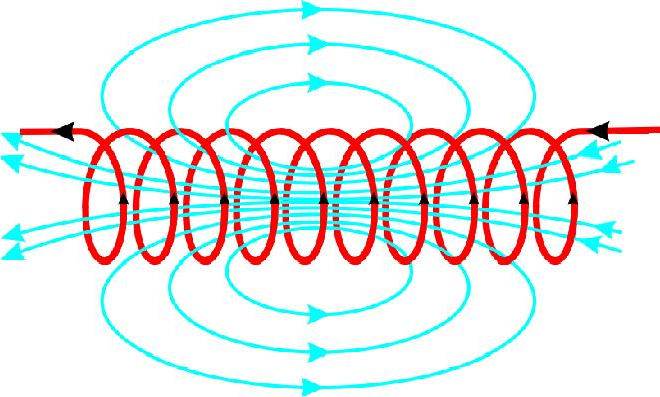
\includegraphics[height=2.5cm]{solenoid_field.png}};
  \node[anchor=south west,text width=8.2cm,font=\small,align=left] at ([xshift=1cm,yshift=0.35cm]current page.south west) {%
    \textbf{Complete classroom deck}: every derivation worked step by step with reasons, labelled diagrams, solved numericals, all textbook questions.\\[4pt]
    \textcolor{gray}{Figures: SCERT Class X Physical Science textbook, pp.\,219--248}};
\end{tikzpicture}
\end{frame}

% =====================================================================
\begin{frame}{Chapter roadmap}
\begin{columns}[T]
\column{0.5\textwidth}
\begin{tcolorbox}[colback=emblue!6,colframe=emblue,title={\textbf{Part A: Currents make magnetic fields}}]
\small
\begin{enumerate}
\item[10.1] Oersted experiment
\item[10.2] Magnetic field, field lines, flux $\Phi$, flux density $B$
\item[10.3] Field of a straight wire, circular coil, solenoid
\end{enumerate}
\end{tcolorbox}
\begin{tcolorbox}[colback=empurple!6,colframe=empurple,title={\textbf{Part B: Fields push on currents}}]
\small
\begin{enumerate}
\item[10.4] $F=qvB\sin\theta$, $F=ILB\sin\theta$, circular motion
\item[10.4] Electric motor
\end{enumerate}
\end{tcolorbox}
\column{0.5\textwidth}
\begin{tcolorbox}[colback=emgreen!6,colframe=emgreen,title={\textbf{Part C: Changing fields make currents}}]
\small
\begin{enumerate}
\item[10.5] Electromagnetic induction
\item[10.5] Faraday's law, Lenz's law
\item[10.5] Derivation: motional emf $\varepsilon=Blv$
\item[10.5] Applications, magnetic levitation
\item[10.5] AC and DC generators
\end{enumerate}
\end{tcolorbox}
\begin{examtip}[How to use this deck]
\small Badges \badge{1M} \badge{2M} \badge{4M} show usual marks. \textbf{Derivation} frames show \emph{step, working, reason}. Answers to \textbf{Teacher asks} appear on the next click.
\end{examtip}
\end{columns}
\end{frame}

% =====================================================================
\begin{frame}{Recall and warm-up}
\begin{columns}[c]
\column{0.52\textwidth}
\begin{itemize}
\item A magnet has two poles, N and S. Like poles repel, unlike poles attract.
\item A freely suspended magnet (compass needle) rests along the \textbf{north--south} direction.
\item A \textbf{field force} acts without contact (gravity, electric, magnetic).
\item Electric current = charges in motion: $I=\dfrac{Q}{t}$.
\item Electric power $P=\varepsilon I$; work $W=Fs$; power $P=Fv$.
\end{itemize}
\column{0.45\textwidth}
\begin{think}[Warm-up questions]
\small
\begin{itemize}
\item How do electric motors and calling bells work?
\item How does an electromagnet work?
\item Is there any relation between electricity and magnetism?
\item Can we produce electricity from magnetism?
\end{itemize}
\end{think}
\end{columns}
\end{frame}

% =====================================================================

\section{Basics first}

% =====================================================================
\begin{frame}{The big picture: one story in three steps}
\centering
\begin{tikzpicture}
\node[story=emblue] (a) at (-5.4,0) {\textbf{\faBolt\ Electric current}\\ moving charges};
\node[story=emteal] (b) at (0,0) {\textbf{\faMagnet\ Magnetic field}\\ appears around the current};
\node[story=emorange] (c) at (5.4,0) {\textbf{\faCog\ Motion}\\ the field pushes things};
\draw[-{Stealth},very thick,emblue] (a) -- node[above,font=\footnotesize,align=center]{\textbf{Part A}\\Oersted} (b);
\draw[-{Stealth},very thick,empurple] (b) -- node[above,font=\footnotesize,align=center]{\textbf{Part B}\\Motor} (c);
\draw[-{Stealth},very thick,emgreen,rounded corners=8pt] (c.south) -- ++(0,-1.3) -- node[below,font=\footnotesize]{\textbf{Part C}: moving a magnet makes current again (Generator)} ($(a.south)+(0,-1.3)$) -- (a.south);
\end{tikzpicture}
\vspace{6pt}
\begin{simple}[Remember this one line]
Electricity and magnetism are \textbf{two faces of the same thing}. Current makes magnetism; magnetism pushes current; changing magnetism makes current.
\end{simple}
\end{frame}
% =====================================================================
\begin{frame}{Basics 1: What is a magnet?}
\begin{columns}[c]
\column{0.5\textwidth}\centering
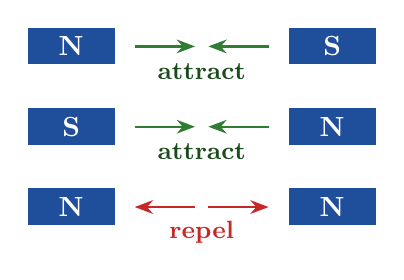
\begin{tikzpicture}[scale=0.85]
\foreach \y/\l/\r in {1.6/N/S,0.4/S/N,-0.8/N/N}{
 \ifx\l N \def\cl{emred}\else\def\cl{emblue}\fi
 \ifx\r N \def\cr{emred}\else\def\cr{emblue}\fi
 \fill[\cl] (-2.6,\y) rectangle (-1.3,\y+0.55); \node[white,font=\bfseries] at (-1.95,\y+0.27) {\l};
 \fill[\cr] (1.3,\y) rectangle (2.6,\y+0.55); \node[white,font=\bfseries] at (1.95,\y+0.27) {\r};}
\draw[-{Stealth},thick,emgreen] (-1.0,1.87) -- (-0.1,1.87); \draw[-{Stealth},thick,emgreen] (1.0,1.87) -- (0.1,1.87);
\node[font=\small\bfseries,emgreen!60!black] at (0,1.5) {attract};
\draw[-{Stealth},thick,emgreen] (-1.0,0.67) -- (-0.1,0.67); \draw[-{Stealth},thick,emgreen] (1.0,0.67) -- (0.1,0.67);
\node[font=\small\bfseries,emgreen!60!black] at (0,0.3) {attract};
\draw[-{Stealth},thick,emred] (-0.1,-0.53) -- (-1.0,-0.53); \draw[-{Stealth},thick,emred] (0.1,-0.53) -- (1.0,-0.53);
\node[font=\small\bfseries,emred] at (0,-0.9) {repel};
\end{tikzpicture}
\column{0.48\textwidth}
\begin{itemize}
\item Every magnet has \textbf{two poles}: North (N) and South (S).
\item \textbf{Unlike} poles attract. \textbf{Like} poles repel.
\item You can never get a single pole: cut a magnet and each piece has both N and S.
\item Magnets attract iron, nickel and cobalt.
\end{itemize}
\begin{simple}[Think of it like this]
A \textbf{compass needle} is a tiny magnet. Its N end always swings to the Earth's geographic north because the Earth itself acts like a giant magnet.
\end{simple}
\end{columns}
\end{frame}
% =====================================================================
\begin{frame}{Basics 2: What is a ``field''?}
\begin{columns}[c]
\column{0.5\textwidth}
\begin{simple}[Kitchen smell analogy]
Cooking in a kitchen: you smell it \textbf{without touching} the food.
\begin{itemize}
\item Strong smell near the stove; weak far away $\Rightarrow$ \textbf{strength} changes with place.
\item Smell drifts \emph{from} the stove \emph{towards} you $\Rightarrow$ it has a \textbf{direction}.
\end{itemize}
\end{simple}
\begin{defn}[Field]
\small Space around an object where it can push or pull other things \textbf{without touching}. A field has \key{strength} and \key{direction} at every point.
\end{defn}
\column{0.46\textwidth}\centering
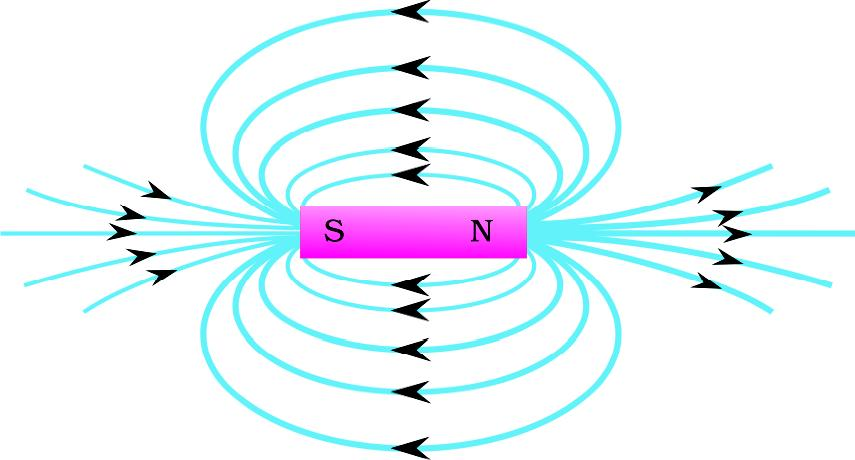
\includegraphics[width=0.95\linewidth]{bar_field.png}\\
{\scriptsize Magnetic field of a bar magnet. Each curve is a \textbf{field line}: the arrow shows the direction; crowded lines mean a stronger field.}
\end{columns}
\end{frame}
% =====================================================================
\begin{frame}{Basics 3: What is electric current?}
\begin{columns}[c]
\column{0.5\textwidth}\centering
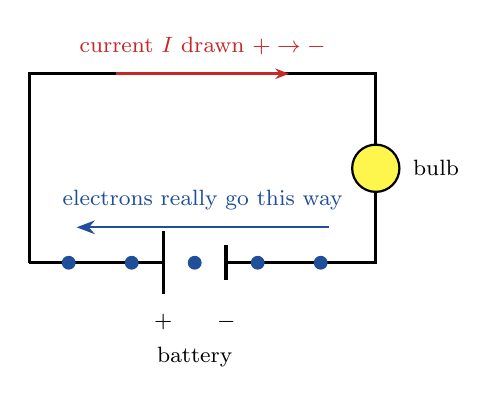
\begin{tikzpicture}
\draw[very thick] (0,0) -- (1.7,0) (2.5,0) -- (4.4,0) -- (4.4,0.9) (4.4,1.5) -- (4.4,2.4) -- (0,2.4) -- (0,0);
\draw[very thick] (1.7,-0.4) -- (1.7,0.4); \draw[ultra thick] (2.5,-0.22) -- (2.5,0.22);
\node[font=\footnotesize] at (1.7,-0.75) {$+$}; \node[font=\footnotesize] at (2.5,-0.75) {$-$};
\node[font=\footnotesize] at (2.1,-1.2) {battery};
\fill[yellow!70,draw=black,thick] (4.4,1.2) circle (0.3); \node[font=\footnotesize,anchor=west] at (4.75,1.2) {bulb};
\draw[cur] (1.1,2.4) -- (3.3,2.4) node[midway,above=3pt,font=\footnotesize,emred]{current $I$ drawn $+\to-$};
\foreach \x in {0.5,1.3,2.1,2.9,3.7}\fill[emblue] (\x,0) circle (2.5pt);
\draw[-{Stealth},emblue,thick] (3.8,0.45) -- (0.6,0.45);
\node[font=\footnotesize,emblue] at (2.2,0.8) {electrons really go this way};
\end{tikzpicture}
\column{0.48\textwidth}
\begin{itemize}
\item Current is the \textbf{flow of charge}, like water flowing in a pipe.
\item Battery = pump, wire = pipe, charge = water.
\end{itemize}
\begin{formula}[Current]
\[I=\frac{Q}{t}\quad\text{unit: ampere (A)}\]
\small $1\,\text{A}=1$ coulomb of charge per second.
\end{formula}
\begin{simple}[Direction convention]
We \textbf{draw} current from $+$ to $-$ (old convention). Electrons really go the other way. Always follow the \textbf{drawn} direction in this chapter.
\end{simple}
\end{columns}
\end{frame}
% =====================================================================
\begin{frame}{Basics 4: Reading arrows into and out of the page}
\begin{columns}[c]
\column{0.5\textwidth}\centering
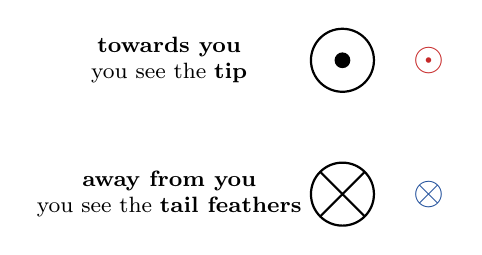
\begin{tikzpicture}
% dart side view
% toward you
\node[font=\footnotesize,align=center] at (0.2,0.2) {\textbf{towards you}\\you see the \textbf{tip}};
\draw[thick,fill=white] (2.4,0.2) circle (0.4); \fill (2.4,0.2) circle (0.1);
\node[font=\Large\bfseries,emred] at (3.5,0.2) {$\odot$};
% away
\node[font=\footnotesize,align=center] at (0.2,-1.5) {\textbf{away from you}\\you see the \textbf{tail feathers}};
\draw[thick,fill=white] (2.4,-1.5) circle (0.4); \draw[thick] (2.4-0.28,-1.5-0.28)--(2.4+0.28,-1.5+0.28) (2.4-0.28,-1.5+0.28)--(2.4+0.28,-1.5-0.28);
\node[font=\Large\bfseries,emblue] at (3.5,-1.5) {$\otimes$};
\end{tikzpicture}
\column{0.48\textwidth}
\begin{itemize}
\item $\odot$ (dot) $\Rightarrow$ pointing \textbf{out of the page}, towards you.
\item $\otimes$ (cross) $\Rightarrow$ pointing \textbf{into the page}, away from you.
\item A page full of $\times$ means a magnetic field going \textbf{into} the page; full of $\cdot$ means \textbf{out}.
\end{itemize}
\begin{simple}[Memory trick]
\textbf{D}ot = \textbf{D}ooming at you (the \emph{tip} is coming at you).\\ \textbf{C}ross = \textbf{C}arrying away (you see the \emph{tail}, it is leaving).
\end{simple}
\end{columns}
\end{frame}
% =====================================================================
\begin{frame}{Basics 5: Your right hand is the tool of this chapter}
\begin{columns}[T]
\column{0.33\textwidth}\centering
\textbf{\color{emblue}Rule 1: thumb rule}\\[2pt]
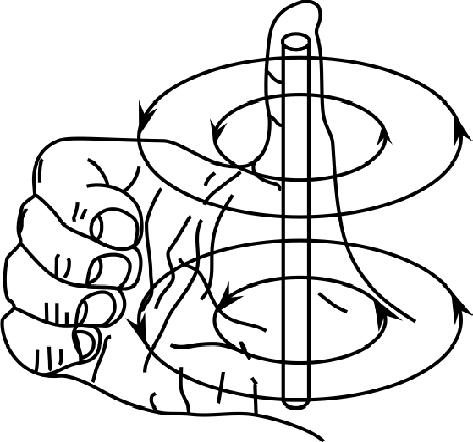
\includegraphics[height=2.4cm]{thumb_rule.png}\\
{\small Straight wire.\\ \textbf{Thumb} = current.\\ \textbf{Curled fingers} = field.}
\column{0.33\textwidth}\centering
\textbf{\color{emteal}Rule 2: coil rule}\\[2pt]
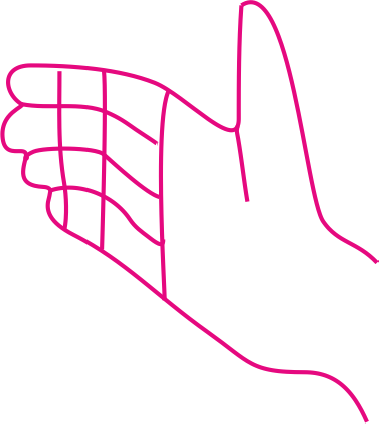
\includegraphics[height=2.4cm]{coil_hand.png}\\
{\small Coil or solenoid.\\ \textbf{Curled fingers} = current.\\ \textbf{Thumb} = N pole.}
\column{0.33\textwidth}\centering
\textbf{\color{emorange}Rule 3: force rule}\\[2pt]

\includegraphics[height=2.4cm]{rh_rule_b.png}\\
{\small Force on current/charge.\\ \textbf{Forefinger} = current $I$ (or $v$),\\ \textbf{middle finger} = field $B$,\\ \textbf{thumb} = force $F$.}
\end{columns}
\vspace{4pt}
\begin{simple}[Always ask: ``What do I know, and what do I want?'']
Know the \textbf{current}, want the \textbf{field}? Rule 1 or 2. Know the \textbf{current and field}, want the \textbf{push}? Rule 3. Use your \textbf{right} hand only.
\end{simple}
\end{frame}
% =====================================================================
\begin{frame}{Basics 6: Symbols and units you will meet}
\centering\renewcommand{\arraystretch}{1.25}
\begin{tabular}{@{}llll@{}}
\toprule
\textbf{Quantity} & \textbf{Symbol} & \textbf{SI unit} & \textbf{In plain words}\\
\midrule
Electric current & $I$ & ampere (A) & how fast charge flows\\
Charge & $q$ or $Q$ & coulomb (C) & amount of electric charge\\
Velocity & $v$ & m/s & speed with direction\\
Magnetic flux density & $B$ & tesla (T) & strength of the field\\
Magnetic flux & $\Phi$ & weber (Wb) & total field passing through an area\\
Force & $F$ & newton (N) & a push or pull\\
Induced emf & $\varepsilon$ & volt (V) & electrical ``push'' that drives current\\
\bottomrule
\end{tabular}
\vspace{4pt}
\begin{examtip}[Unit tip]
$1\,\text{T}=1\,\text{Wb/m}^2$. Convert first: cm $\to$ m, cm$^2\to$ m$^2$ (divide by $10^4$), before substituting into formulas.
\end{examtip}
\end{frame}
% =====================================================================
\begin{frame}{Maths 1: Powers of ten (scientific notation)}
\begin{columns}[T]
\column{0.5\textwidth}
\begin{simple}[Why?]
Physics numbers can be huge or tiny. Charge of a proton: $0.00000000000000000016$ C. Write it as $\mathbf{1.6\times10^{-19}}$ C.
\end{simple}
\begin{itemize}
\item $10^{3}=1000$,\; $10^{-3}=\dfrac{1}{1000}=0.001$
\item Move the point \textbf{left} $\Rightarrow$ power goes \textbf{up}; move \textbf{right} $\Rightarrow$ power goes \textbf{down}.
\end{itemize}
\column{0.48\textwidth}
\begin{formula}[Rules]
\[10^{a}\times10^{b}=10^{a+b}\qquad\frac{10^{a}}{10^{b}}=10^{a-b}\]
\end{formula}
\begin{answer}[Worked example]
$(2\times10^{6})\times(1.6\times10^{-19})\times0.5$\\
Numbers: $2\times1.6\times0.5=1.6$\\
Powers: $10^{6-19}=10^{-13}$\\
Answer: $\mathbf{1.6\times10^{-13}}$
\end{answer}
\end{columns}
\end{frame}
% =====================================================================
\begin{frame}{Maths 2: Changing units before you calculate}
\centering\renewcommand{\arraystretch}{1.25}
\begin{tabular}{@{}lll@{}}
\toprule
\textbf{Change} & \textbf{How} & \textbf{Example}\\
\midrule
cm $\to$ m & divide by 100 & $20\ \text{cm}=0.2$ m\\
mm $\to$ m & divide by 1000 & $5.7$ mm $=5.7\times10^{-3}$ m\\
cm$^2\to$ m$^2$ & divide by $10^{4}$ (not 100!) & $4\ \text{cm}^2=4\times10^{-4}$ m$^2$\\
minutes $\to$ s & multiply by 60 & $0.2$ min $=12$ s\\
\bottomrule
\end{tabular}
\vspace{6pt}
\begin{simple}[Why $10^4$ for area?]
$1\ \text{cm}=\frac{1}{100}$ m, so $1\ \text{cm}^2=\frac{1}{100}\times\frac{1}{100}=\frac{1}{10\,000}$ m$^2$. Area squares the conversion factor.
\end{simple}
\end{frame}
% =====================================================================
\begin{frame}{Maths 3: Rearranging a formula (the balance method)}
\begin{columns}[T]
\column{0.5\textwidth}
\begin{simple}[Golden rule]
An equation is a balance. Whatever you do to one side, do the \textbf{same} to the other.
\end{simple}
Start with $F=ILB$.
\begin{itemize}
\item Find $B$: divide both sides by $IL$ $\Rightarrow$ $B=\dfrac{F}{IL}$
\item Find $I$: divide both sides by $LB$ $\Rightarrow$ $I=\dfrac{F}{LB}$
\item Find $L$: divide both sides by $IB$ $\Rightarrow$ $L=\dfrac{F}{IB}$
\end{itemize}
\column{0.48\textwidth}
\begin{answer}[Example from the chapter]
$r=\dfrac{mv}{Bq}$. Find $v$.\\[3pt]
Multiply both sides by $Bq$: $rBq=mv$\\
Divide both sides by $m$: $v=\dfrac{rBq}{m}$
\end{answer}
\begin{examtip}[Steps for every numerical]
1. Write the formula. 2. Convert units. 3. Rearrange if needed. 4. Substitute. 5. Calculate and write the \textbf{unit}.
\end{examtip}
\end{columns}
\end{frame}
% =====================================================================
\begin{frame}{Maths 4: Sine and cosine of an angle}
\begin{columns}[c]
\column{0.42\textwidth}\centering
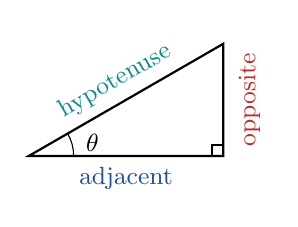
\begin{tikzpicture}[scale=0.95]
\draw[thick] (0,0) -- (2.6,0) -- (2.6,1.5) -- cycle;
\draw[thick] (2.45,0) -- (2.45,0.15) -- (2.6,0.15);
\draw (0.6,0) arc (0:30:0.6); \node[font=\small] at (0.85,0.17) {$\theta$};
\node[font=\small,emblue] at (1.3,-0.3) {adjacent};
\node[font=\small,emred,rotate=90] at (2.95,0.75) {opposite};
\node[font=\small,emteal,rotate=30] at (1.15,1.0) {hypotenuse};
\end{tikzpicture}
{\small$\sin\theta=\dfrac{\text{opposite}}{\text{hypotenuse}}$\\[4pt]$\cos\theta=\dfrac{\text{adjacent}}{\text{hypotenuse}}$}
\column{0.56\textwidth}
\small\centering\renewcommand{\arraystretch}{1.2}
\begin{tabular}{@{}c|ccccc@{}}
$\theta$ & $0^\circ$ & $30^\circ$ & $45^\circ$ & $60^\circ$ & $90^\circ$\\\hline
$\sin\theta$ & $0$ & $\tfrac12$ & $\tfrac{1}{\sqrt2}$ & $\tfrac{\sqrt3}{2}$ & $1$\\
$\cos\theta$ & $1$ & $\tfrac{\sqrt3}{2}$ & $\tfrac{1}{\sqrt2}$ & $\tfrac12$ & $0$\\
\end{tabular}
\vspace{4pt}
\begin{simple}[Where we use them]
$F=qvB\sin\theta$: $\theta$ is the angle between $v$ and $B$. At $90^\circ$ the force is maximum; at $0^\circ$ it is zero.\\
$\Phi=BA\cos\theta$: $\theta$ is the angle between $B$ and the \textbf{normal} to the plane. At $0^\circ$ the flux is maximum.
\end{simple}
\end{columns}
\end{frame}
% =====================================================================
\begin{frame}{Maths 5: Area, circles and time period}
\begin{columns}[T]
\column{0.5\textwidth}
\begin{formula}[Shapes]
\small Rectangle: $A=\text{length}\times\text{breadth}$\\
Circle: $A=\pi r^{2}$, circumference $=2\pi r$ ($\pi\approx3.14$)
\end{formula}
\begin{answer}[Example]
Loop of radius $0.1$ m: $A=3.14\times0.1^{2}=0.0314$ m$^{2}$.
\end{answer}
\column{0.48\textwidth}
\begin{formula}[Speed, distance, time]
\[v=\frac{\text{distance}}{\text{time}}\;\Rightarrow\;\text{time}=\frac{\text{distance}}{v}\]
\end{formula}
\begin{simple}[Time period $T$]
Time for one full circle: $T=\dfrac{2\pi r}{v}$. We use this in the circular-path derivation.
\end{simple}
\end{columns}
\end{frame}
% =====================================================================
\begin{frame}{Maths 6: ``Change'' and ``rate of change'' ($\Delta$)}
\begin{columns}[c]
\column{0.5\textwidth}
\begin{itemize}
\item $\Delta$ (delta) means \textbf{change} = final $-$ initial.
\item $\Delta\Phi=\Phi_{\text{final}}-\Phi_{\text{initial}}$,\quad $\Delta t=t_{\text{final}}-t_{\text{initial}}$
\item \textbf{Rate of change} = change $\div$ time taken, e.g.\ $\varepsilon=\dfrac{\Delta\Phi}{\Delta t}$.
\end{itemize}
\begin{answer}[Example]
Flux falls from $0.5$ Wb to $0.1$ Wb in $0.2$ s.\\
$\Delta\Phi=0.1-0.5=-0.4$ Wb\\
$|\varepsilon|=\dfrac{0.4}{0.2}=\mathbf{2}$ V
\end{answer}
\column{0.46\textwidth}\centering
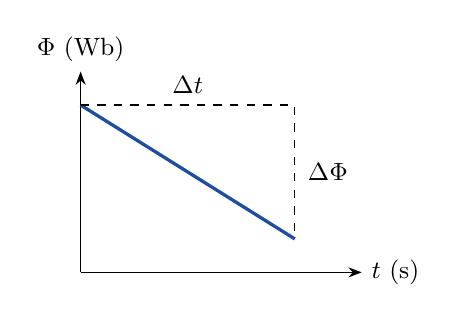
\begin{tikzpicture}[scale=0.85]
\draw[-{Stealth}] (0,0) -- (4.2,0) node[right,font=\small]{$t$ (s)};
\draw[-{Stealth}] (0,0) -- (0,3) node[above,font=\small]{$\Phi$ (Wb)};
\draw[very thick,emblue] (0,2.5) -- (3.2,0.5);
\draw[dashed] (0,2.5) -- (3.2,2.5) -- (3.2,0.5);
\node[font=\small] at (1.6,2.8) {$\Delta t$}; \node[font=\small,anchor=west] at (3.25,1.5) {$\Delta\Phi$};
\end{tikzpicture}\\
{\small Slope of a flux--time graph = $\dfrac{\Delta\Phi}{\Delta t}$ = induced emf. A steeper line means a bigger emf; a flat line means zero emf.}
\end{columns}
\end{frame}
% =====================================================================
\begin{frame}{Maths 7: Proportion, ``if this doubles, what happens?''}
\begin{columns}[T]
\column{0.55\textwidth}
\renewcommand{\arraystretch}{1.3}\small
\begin{tabular}{@{}lll@{}}
\toprule
\textbf{Formula} & \textbf{If this doubles\ldots} & \textbf{That}\\
\midrule
$F=ILB$ & $B$ doubles & $F$ doubles\\
$F=ILB$ & $I$ and $L$ both double & $F$ becomes $4\times$\\
$r=\dfrac{mv}{Bq}$ & $B$ doubles & $r$ \textbf{halves}\\
$\varepsilon=Blv$ & $v$ doubles & $\varepsilon$ doubles\\
$\Phi=BA\cos\theta$ & $A$ doubles & $\Phi$ doubles\\
\bottomrule
\end{tabular}
\column{0.43\textwidth}
\begin{simple}[Two kinds of relation]
\textbf{Direct} ($F\propto B$): both grow together.\\
\textbf{Inverse} ($r\propto\frac{1}{B}$): one grows, the other shrinks.
\end{simple}
\begin{examtip}
Spot the variable on top (direct) or underneath (inverse) in the formula.
\end{examtip}
\end{columns}
\end{frame}
% =====================================================================
\begin{frame}{Maths check: try these}
\small
\begin{columns}[T]
\column{0.5\textwidth}
\begin{think}[Quick maths drill]
\begin{enumerate}
\item Write $0.0005$ in powers of ten.
\item Convert $50$ cm$^2$ to m$^2$.
\item $F=ILB$: find $L$ if $F=6$ N, $I=3$ A, $B=0.5$ T.
\item Value of $\sin30^\circ$ and $\cos60^\circ$?
\item Flux changes by $0.6$ Wb in $0.3$ s. Find $\varepsilon$.
\end{enumerate}
\end{think}
\column{0.46\textwidth}
\uncover<2->{\begin{answer}[Answers]
\begin{enumerate}
\item $5\times10^{-4}$
\item $5\times10^{-3}$ m$^2$
\item $L=\dfrac{6}{3\times0.5}=4$ m
\item both $\tfrac12$
\item $\varepsilon=\dfrac{0.6}{0.3}=2$ V
\end{enumerate}
\end{answer}}
\end{columns}
\end{frame}
% =====================================================================
\begin{frame}{Quick check before we start}
\small
\begin{columns}[T]
\column{0.5\textwidth}
\begin{think}[Try these (answers on the next click)]
\begin{enumerate}
\item Two N poles are brought close. Attract or repel?
\item Charge $6$ C flows in $2$ s. Find the current.
\item An arrow shows $\otimes$. Is it going into or out of the page?
\item Which hand do we use for the rules?
\end{enumerate}
\end{think}
\column{0.46\textwidth}
\uncover<2->{\begin{answer}[Answers]
\begin{enumerate}
\item Repel (like poles).
\item $I=Q/t=6/2=3$ A.
\item Into the page.
\item The right hand.
\end{enumerate}
\end{answer}}
\end{columns}
\end{frame}

\section{Part A: Magnetic field}
% =====================================================================
\begin{frame}{Part A: Currents make magnetic fields}
\begin{goals}
\large\begin{itemize}
\item Describe what Oersted observed and what it proves.
\item Draw and read \textbf{magnetic field lines}; tell a strong field from a weak one.
\item Explain \textbf{flux} $\Phi$ and \textbf{flux density} $B$, and use $\Phi=BA\cos\theta$.
\item Find the field direction around a wire, a coil and a solenoid with the \textbf{right hand rule}.
\end{itemize}
\end{goals}
\end{frame}

\begin{frame}{10.1 Oersted experiment (Activity 1) \hfill \badge{2M} \badge{4M}}
\begin{columns}[T]
\column{0.56\textwidth}
\centering
\figlab{oersted_setup.png}{width=\linewidth}{
\draw[fptr] (0.30,1.12) node[flab,anchor=south east]{copper wire (24 gauge)} -- (0.36,0.82);
\draw[fptr] (0.36,1.12) node[flab,anchor=south west]{wooden sticks} -- (0.50,0.95);
\draw[fptr] (0.36,1.12) -- (0.27,0.62);
\draw[fptr] (0.30,0.20) node[flab,anchor=north]{magnetic compass} -- (0.40,0.60);
\draw[fptr] (0.85,1.10) node[flab,anchor=south]{battery (3 V)} -- (0.66,0.78);
\draw[fptr] (0.72,0.10) node[flab,anchor=north]{key} -- (0.54,0.40);
\draw[fptr] (0.05,0.05) node[flab,anchor=north]{thermocol sheet} -- (0.15,0.40);}\\[12pt]
{\scriptsize fig-1: current-carrying wire above a compass}
\column{0.42\textwidth}
\small
\begin{enumerate}
\item Wire stretched through slits of two sticks, in series with battery and key. Compass below the wire.
\item Bring a bar magnet near: needle deflects (magnetic force).
\item Remove the magnet, switch \textbf{on}: needle \textbf{deflects again}!
\item Switch off: needle returns to N--S.
\end{enumerate}
\begin{answer}[Conclusion]
\small A \textbf{current-carrying wire produces a magnetic field} around it. Electricity and magnetism are related.
\end{answer}
\end{columns}
\end{frame}

% =====================================================================
\begin{frame}{Do you know? Hans Christian Oersted \hfill \badge{1M}}
\begin{columns}[c]
\column{0.26\textwidth}\centering
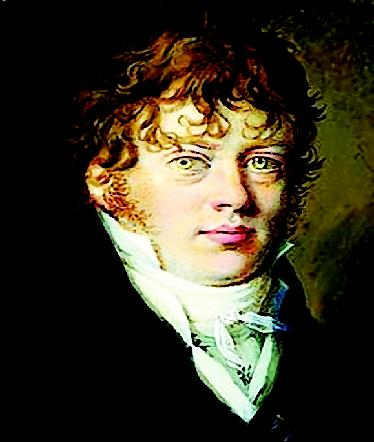
\includegraphics[width=0.9\linewidth]{oersted.png}\\{\scriptsize H.\,C.\ Oersted (1777--1851)}
\column{0.72\textwidth}
\begin{itemize}
\item In a lecture in April 1820 he placed a compass needle under a wire and switched on the current: the needle \textbf{deflected}.
\item Showed that electricity and magnetism are \textbf{interconnected}: the start of \key{electromagnetism}.
\item Led to the dynamo, the electric motor, radio, television and fibre optics.
\item The unit of magnetic field strength is named \imp{oersted} in his honour.
\end{itemize}
\end{columns}
\end{frame}

% =====================================================================
\begin{frame}{10.2 Magnetic field of a bar magnet (Activity 2) \hfill \badge{1M} \badge{2M}}
\begin{columns}[T]
\column{0.55\textwidth}
\begin{activity}[Activity 2: compass around a bar magnet]
\small Place a compass at many points around a bar magnet on paper. Mark the direction of the needle at each point (S $\to$ N of the needle).
\end{activity}
\small
\begin{itemize}
\item The needle points in \textbf{different directions} at different places $\Rightarrow$ the field has \textbf{direction} that varies from point to point.
\item Far from the magnet the needle points almost N--S $\Rightarrow$ \textbf{strength} decreases with distance.
\item Above the magnet the needle is also deflected $\Rightarrow$ the field is \textbf{three-dimensional}.
\end{itemize}
\column{0.43\textwidth}
\begin{defn}[Field]
\small A region where a force acts on an object \textbf{without physical contact}.
\end{defn}
\begin{defn}[Magnetic field]
\small The region surrounding a magnet in which its magnetic force can be felt. It is characterised by \key{strength} and \key{direction}.
\end{defn}
\end{columns}
\end{frame}

% =====================================================================
\begin{frame}{10.2.1 Magnetic field lines (Activity 3) \hfill \badge{1M} \badge{2M} \badge{Diagram}}
\begin{columns}[c]
\column{0.5\textwidth}\centering
\figlab{bar_field.png}{width=\linewidth}{
\draw[fptr] (0.12,1.08) node[flab,anchor=south]{field line} -- (0.30,0.93);
\draw[fptr] (0.88,1.08) node[flab,anchor=south]{lines crowded near poles (strong)} -- (0.72,0.62);
\draw[fptr] (0.50,-0.10) node[flab,anchor=north]{lines far apart (weak)} -- (0.50,0.04);}\\[12pt]
{\scriptsize fig-2: field lines of a bar magnet (outside: N $\to$ S)}
\column{0.48\textwidth}
\small
\textbf{Plotting:} put the compass at N, mark a dot at the tip of the needle, move the compass to the dot, repeat until you reach S. Join the dots.
\begin{itemize}
\item Field lines are \textbf{imaginary} curves.
\item \key{Tangent} at any point gives the direction of the field.
\item \textbf{Crowded} lines $\Rightarrow$ strong field; \textbf{spread} lines $\Rightarrow$ weak field.
\item \key{Non-uniform field}: strength \textbf{or} direction changes.\\ \key{Uniform field}: strength \textbf{and} direction constant (parallel, equally spaced lines).
\end{itemize}
\end{columns}
\end{frame}

% =====================================================================
\begin{frame}{10.2.2 Magnetic flux and flux density \hfill \badge{1M} \badge{2M}}
\begin{columns}[c]
\column{0.44\textwidth}\centering
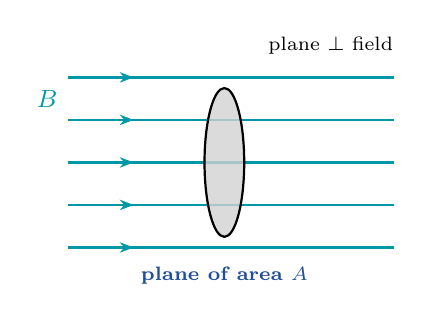
\begin{tikzpicture}[scale=0.9]
\foreach \y in {-1.2,-0.6,0,0.6,1.2} \draw[fl=0.2] (-2.2,\y) -- (2.4,\y);
\fill[gray!35,opacity=0.8] (0,0) ellipse (0.28 and 1.05);
\draw[thick] (0,0) ellipse (0.28 and 1.05);
\node[flab] at (0.0,-1.6) {plane of area $A$};
\node[font=\small\bfseries,fieldc] at (-2.5,0.9) {$B$};
\node[font=\scriptsize,align=center] at (1.5,1.65) {plane $\perp$ field};
\end{tikzpicture}\\
{\scriptsize fig-3(a): lines crossing a plane placed perpendicular to a uniform field}
\column{0.54\textwidth}
\begin{defn}[Magnetic flux $\Phi$]
\small The number of field lines passing through a plane of area $A$ held \textbf{perpendicular} to the field. SI unit: \key{weber (Wb)}.
\end{defn}
\begin{defn}[Magnetic flux density $B$]
\small Flux passing through \textbf{unit area} held perpendicular to the field. Also called \key{magnetic induction}.
\[B=\frac{\Phi}{A}\qquad\text{unit: Wb/m}^2=\text{tesla (T)}\]
\end{defn}
\end{columns}
\end{frame}

% =====================================================================
\begin{frame}[shrink=8]{Flux in simple words: rain through a window}
\begin{columns}[c]
\column{0.6\textwidth}\centering
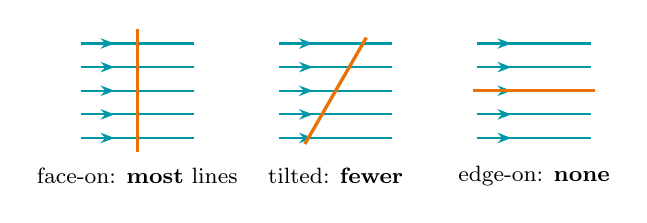
\begin{tikzpicture}[scale=0.6]
\foreach \ang/\xo/\lab in {90/0/{face-on: \textbf{most} lines},60/4.2/{tilted: \textbf{fewer}},0/8.4/{edge-on: \textbf{none}}}{
 \foreach \y in {-1.0,-0.5,0,0.5,1.0} \draw[fl=0.3] (\xo-1.2,\y) -- (\xo+1.2,\y);
 \draw[very thick,emorange] ($(\xo,0)+(\ang:1.3)$) -- ($(\xo,0)-(\ang:1.3)$);
 \node[font=\footnotesize,align=center] at (\xo,-1.8) {\lab};}
\end{tikzpicture}\\
{\scriptsize Orange line = the window seen edge-on; blue lines = field lines (rain).}
\column{0.38\textwidth}
\begin{simple}[Analogy]
Rain = field lines. Window = area $A$.
\begin{itemize}
\item Hold the window \textbf{face-on}: the most rain passes.
\item \textbf{Tilt} it: less passes.
\item \textbf{Edge-on}: no rain passes.
\end{itemize}
\textbf{Flux $\Phi$} = how much rain passes. \textbf{Flux density $B$} = how heavy the rain is.
\end{simple}
\end{columns}
\end{frame}

% =====================================================================
\begin{frame}[shrink=15]{Derivation 1: flux through a tilted plane, $\Phi=BA\cos\theta$ \hfill \badge{2M}}
\begin{columns}[T]
\column{0.4\textwidth}\centering
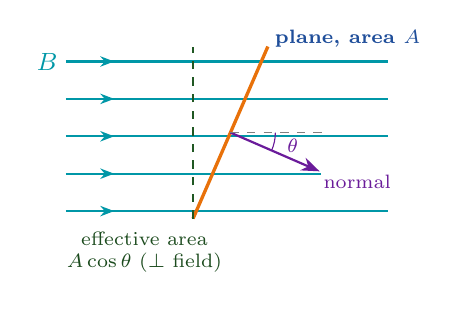
\begin{tikzpicture}[scale=0.95]
\foreach \y in {0.2,0.7,1.2,1.7,2.2} \draw[fl=0.15] (-0.5,\y) -- (3.8,\y);
\node[font=\small\bfseries,fieldc] at (-0.75,2.2) {$B$};
% tilted plane (edge view)
\draw[very thick,emorange] (1.2,0.1) -- (2.2,2.4);
\node[flab,anchor=west] at (2.25,2.5) {plane, area $A$};
% normal
\coordinate (C) at (1.7,1.25);
\draw[-{Stealth},thick,empurple] (C) -- ($(C)+(-23.5:1.3)$) node[below right,font=\scriptsize,empurple,fill=white,inner sep=1pt]{normal};
\draw[dashed,gray] (C) -- ($(C)+(1.3,0)$);
\draw[empurple] ($(C)+(0.6,0)$) arc (0:-23.5:0.6); \node[font=\scriptsize,empurple] at ($(C)+(-12:0.85)$) {$\theta$};
% projection perpendicular to field
\draw[thick,dashed,emgreen!70!black] (1.2,0.1) -- (1.2,2.4);
\node[font=\scriptsize,emgreen!60!black,align=center] at (0.55,-0.35) {effective area\\$A\cos\theta$ ($\perp$ field)};
\end{tikzpicture}\\
{\scriptsize fig-3(b): edge view of the plane}
\column{0.58\textwidth}
\begin{steps}[3.3cm]
\stp1 & B=\frac{\Phi}{A_{\perp}} & $B$ is always defined with the area \textbf{perpendicular} to the field\\
\stp2 & A_{\perp}=A\cos\theta & $\theta$ = angle between $B$ and the normal; only this part of the plane faces the field\\
\stp3 & B=\frac{\Phi}{A\cos\theta} & substitute step 2 in step 1\\
\stp4 & \Phi=BA\cos\theta & multiply both sides by $A\cos\theta$\\
\end{steps}
\begin{formula}[Special cases]
\small $\theta=0^\circ$ (plane $\perp$ field): $\Phi=BA$ (maximum)\\
$\theta=90^\circ$ (plane $\parallel$ field): $\Phi=BA\cos90^\circ=0$
\end{formula}
\end{columns}
\end{frame}

% =====================================================================
\begin{frame}{Solved numericals: flux and flux density \hfill \badge{2M}}
\small
\begin{columns}[T]
\column{0.5\textwidth}
\begin{tcolorbox}[colback=emblue!4,colframe=emblue,title={\textbf{Q1.} $B=0.5$ T through a loop of area $0.02$ m$^2$, loop $\perp$ field. Find $\Phi$.}]
\stp1 Plane $\perp$ field $\Rightarrow\theta=0^\circ$, $\cos0^\circ=1$.\\
\stp2 $\Phi=BA=0.5\times0.02=\boxed{0.01\ \text{Wb}}$
\end{tcolorbox}
\pause
\begin{tcolorbox}[colback=emblue!4,colframe=emblue,title={\textbf{Q2.} Same loop turned so the normal makes $60^\circ$ with $B$.}]
\stp1 $\Phi=BA\cos60^\circ=0.01\times\frac12=\boxed{0.005\ \text{Wb}}$
\end{tcolorbox}
\column{0.5\textwidth}
\pause
\begin{tcolorbox}[colback=emgreen!5,colframe=emgreen,title={\textbf{Q3.} Flux of $2\times10^{-3}$ Wb crosses $4$ cm$^2$ normally. Find $B$.}]
\stp1 $A=4\ \text{cm}^2=4\times10^{-4}$ m$^2$ \;(1 cm$^2=10^{-4}$ m$^2$)\\[2pt]
\stp2 $B=\dfrac{\Phi}{A}=\dfrac{2\times10^{-3}}{4\times10^{-4}}=\boxed{5\ \text{T}}$
\end{tcolorbox}
\pause
\begin{think}[Textbook question]
\small What is the flux through a plane held \textbf{parallel} to the field?\\
\onslide<5->{\textbf{Zero}: no field line crosses it ($\theta=90^\circ$).}
\end{think}
\end{columns}
\end{frame}

% =====================================================================
\begin{frame}{10.3.1 Field of a straight current-carrying wire (Activity 4) \hfill \badge{2M} \badge{4M}}
\begin{columns}[T]
\column{0.42\textwidth}\centering
\figlab{wire_setup.png}{height=0.6\textheight}{
\draw[fptr] (0.30,0.97) node[flab,anchor=south]{retort stand} -- (0.58,0.92);
\draw[fptr] (1.05,0.97) node[flab,anchor=south]{vertical wire} -- (0.84,0.75);
\draw[fptr] (1.02,0.02) node[flab,anchor=north]{compass needles} -- (0.85,0.51);
\draw[fptr] (0.62,0.02) node[flab,anchor=north]{plank} -- (0.70,0.50);
\draw[fptr] (-0.05,0.70) node[flab,anchor=east]{battery} -- (0.27,0.52);
\draw[fptr] (-0.05,0.45) node[flab,anchor=east]{switch} -- (0.38,0.49);
\draw[fptr] (-0.05,0.25) node[flab,anchor=east]{table} -- (0.10,0.35);}\\
{\scriptsize fig-4(a)}
\column{0.56\textwidth}
\small
\begin{enumerate}
\item Pass a vertical wire through a hole in a plank; place 6--10 compass needles on a circle around the hole.
\item Switch on (3 V battery).
\item The needles set along \textbf{tangents to the circle}.
\item Sprinkle iron filings: they form \textbf{concentric circles}.
\end{enumerate}
\begin{answer}[Conclusion]
\small Field lines of a straight wire are \textbf{concentric circles} centred on the wire, in a plane perpendicular to it. They are \imp{closed loops}. The field is stronger near the wire (circles closer).
\end{answer}
\end{columns}
\end{frame}

% =====================================================================
\begin{frame}[shrink=6]{Direction of the field: right hand thumb rule \hfill \badge{1M} \badge{2M}}
\begin{columns}[c]
\column{0.28\textwidth}\centering
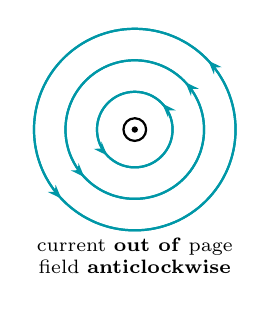
\begin{tikzpicture}[scale=0.8]
\foreach \r/\p in {0.6/0.12,1.1/0.12,1.6/0.12} \draw[fl=\p] (0,0) circle (\r);
\foreach \r/\p in {0.6/0.62,1.1/0.62,1.6/0.62} \draw[fieldc,thick,postaction={decorate},decoration={markings,mark=at position \p with {\arrow{Stealth[length=5pt]}}}] (0,0) circle (\r);
\outpage{(0,0)}
\node[font=\scriptsize,align=center] at (0,-2.0) {current \textbf{out of} page\\field \textbf{anticlockwise}};
\end{tikzpicture}\\{\scriptsize fig-4(b)}
\column{0.28\textwidth}\centering
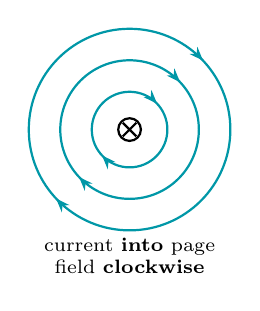
\begin{tikzpicture}[scale=0.8]
\foreach \r in {0.6,1.1,1.6} \draw[fieldc,thick,postaction={decorate},decoration={markings,mark=at position 0.12 with {\arrowreversed{Stealth[length=5pt]}},mark=at position 0.62 with {\arrowreversed{Stealth[length=5pt]}}}] (0,0) circle (\r);
\inpage{(0,0)}
\node[font=\scriptsize,align=center] at (0,-2.0) {current \textbf{into} page\\field \textbf{clockwise}};
\end{tikzpicture}\\{\scriptsize fig-4(c)}
\column{0.42\textwidth}\centering
\figlab{thumb_rule.png}{width=0.62\linewidth}{
\draw[cur] (0.63,0.80) -- (0.63,1.08) node[above,font=\scriptsize\bfseries,emred]{thumb: current $I$};
\draw[fptr] (1.10,0.55) node[flab,anchor=west,align=left]{fingers:\\field $B$} -- (0.97,0.72);}\\
{\scriptsize fig-4(d)}
\begin{defn}[Right hand thumb rule]
\small Grasp the wire with the right hand with the \textbf{thumb along the current}; the \textbf{curled fingers} give the direction of the field lines.
\end{defn}
\end{columns}
\vspace{2pt}
{\scriptsize Symbols: $\odot$ current/field out of the page (arrow tip);\quad $\otimes$ into the page (arrow tail).}
\end{frame}

% =====================================================================
\begin{frame}{10.3.2 Field of a circular coil (Activity 5) \hfill \badge{2M} \badge{4M}}
\begin{columns}[T]
\column{0.42\textwidth}\centering
\figlab{coil_setup.png}{width=0.95\linewidth}{
\draw[fptr] (0.10,1.08) node[flab,anchor=south]{circular coil (4--5 turns)} -- (0.34,0.90);
\draw[fptr] (0.62,1.08) node[flab,anchor=south]{compass at centre} -- (0.50,0.70);
\draw[fptr] (0.72,-0.06) node[flab,anchor=north]{to current supply} -- (0.88,0.58);
\draw[fptr] (0.72,-0.06) -- (0.64,0.30);}\\[8pt]
{\scriptsize fig-5(a)}
\column{0.56\textwidth}
\small
\begin{itemize}
\item Plot field lines with a compass around the coil.
\item At the centre the needle points \textbf{perpendicular to the plane of the coil}: the field there is along the axis.
\item Bring a compass near one face: its S pole points to the face $\Rightarrow$ that face acts as a \textbf{N pole}.
\end{itemize}
\begin{defn}[Right hand rule for a coil]
\small Curl the right-hand fingers along the \textbf{current}; the \textbf{thumb} gives the direction of the \textbf{field} (points out of the N face).
\end{defn}
\end{columns}
\end{frame}

\begin{frame}{Coil: which face is North? \hfill \badge{1M} \badge{2M}}
\begin{columns}[c]
\column{0.3\textwidth}\centering
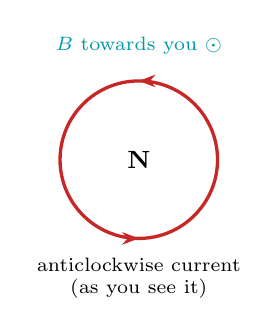
\begin{tikzpicture}
\draw[emred,very thick,postaction={decorate},decoration={markings,mark=at position 0.25 with {\arrow{Stealth[length=6pt]}},mark=at position 0.75 with {\arrow{Stealth[length=6pt]}}}] (0,0) circle (1);
\node[font=\small\bfseries] at (0,0) {N};
\node[font=\scriptsize,align=center] at (0,-1.5) {anticlockwise current\\(as you see it)};
\node[font=\scriptsize,align=center,fieldc] at (0,1.45) {$B$ towards you $\odot$};
\end{tikzpicture}
\column{0.3\textwidth}\centering
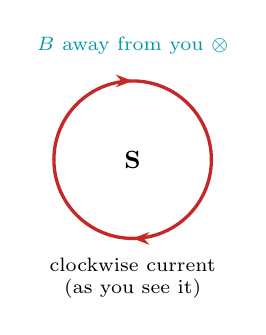
\begin{tikzpicture}
\draw[emred,very thick,postaction={decorate},decoration={markings,mark=at position 0.25 with {\arrowreversed{Stealth[length=6pt]}},mark=at position 0.75 with {\arrowreversed{Stealth[length=6pt]}}}] (0,0) circle (1);
\node[font=\small\bfseries] at (0,0) {S};
\node[font=\scriptsize,align=center] at (0,-1.5) {clockwise current\\(as you see it)};
\node[font=\scriptsize,align=center,fieldc] at (0,1.45) {$B$ away from you $\otimes$};
\end{tikzpicture}
\column{0.38\textwidth}\centering
\figlab{coil_hand.png}{width=0.52\linewidth}{
\draw[fptr] (1.08,0.95) node[flab,anchor=west]{thumb: $B$} -- (0.70,0.97);
\draw[fptr] (-0.08,0.45) node[flab,anchor=east,align=right]{fingers:\\current $I$} -- (0.12,0.70);}\\
{\scriptsize fig-5(b): right hand rule for a coil}
\begin{examtip}
\small Memory aid: letters \textbf{N} and \textbf{S} drawn with arrows at their ends run anticlockwise and clockwise respectively.
\end{examtip}
\end{columns}
\end{frame}

% =====================================================================
\begin{frame}{10.3.3 Field of a solenoid (Activity 6) \hfill \badge{2M} \badge{4M}}
\begin{columns}[T]
\column{0.4\textwidth}\centering
\figlab{solenoid_setup.png}{height=0.26\textheight}{
\draw[fptr] (0.12,1.08) node[flab,anchor=south]{solenoid (long helix)} -- (0.36,0.84);
\draw[fptr] (0.70,-0.05) node[flab,anchor=north]{to current supply} -- (0.83,0.52);}\\[4pt]
{\scriptsize fig-6(a)}\\[8pt]
\figlab{solenoid_field.png}{height=0.27\textheight}{
\node[font=\small\bfseries,emred] at (-0.04,0.5) {N};
\node[font=\small\bfseries,emred] at (1.04,0.5) {S};
\node[font=\scriptsize\bfseries,emred] at (0.08,0.80) {$I$};
\node[font=\scriptsize\bfseries,emred] at (0.93,0.80) {$I$};
}\\[2pt]
{\scriptsize fig-6(b): field lines (iron filings)}
\column{0.58\textwidth}
\small
\begin{defn}[Solenoid]
\small A long wire wound in a \textbf{close-packed helix}.
\end{defn}
\begin{itemize}
\item Iron filings show a pattern like that of a \textbf{bar magnet}: a solenoid behaves like a bar magnet.
\item One end is N, the other S (find with the right hand rule).
\item Outside: field lines go \textbf{N $\to$ S}; inside: \textbf{S $\to$ N}, strong and nearly uniform (parallel lines).
\item Lines outside are continuous with those inside $\Rightarrow$ field lines are \imp{closed loops}. Same for a bar magnet.
\end{itemize}
\begin{answer}[Big idea]
\small Moving charges (currents) produce magnetic fields.
\end{answer}
\end{columns}
\end{frame}

% =====================================================================
\section{Part B: Magnetic force}
% =====================================================================
\begin{frame}{Part B: Fields push on currents}
\begin{goals}
\large\begin{itemize}
\item Find the \textbf{direction and size} of the force on a moving charge, $F=qvB\sin\theta$.
\item Show why a charge in a field moves in a \textbf{circle}: $r=mv/Bq$.
\item Derive $F=ILB\sin\theta$ for a current-carrying wire.
\item Explain how an \textbf{electric motor} keeps turning.
\end{itemize}
\end{goals}
\end{frame}

\begin{frame}{10.4 Force on a moving charge (Activity 7) \hfill \badge{1M} \badge{2M}}
\begin{columns}[T]
\column{0.52\textwidth}
\begin{activity}[Activity 7: magnet near an old CRT TV]
\small The picture gets \textbf{distorted}; move the magnet away and it clears.
\end{activity}
\small The picture is made by a beam of \textbf{moving electrons}. The magnetic field exerts a force on them and changes their path: the \key{magnetic force}.
\begin{formula}[Magnetic force on a charge]
\[F=qvB\quad(\vec v\perp\vec B)\qquad F=qvB\sin\theta\]
$\theta$ = angle between $\vec v$ and $\vec B$.
\end{formula}
\column{0.46\textwidth}\centering
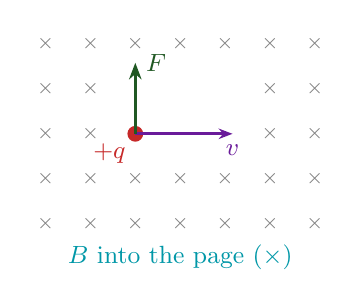
\begin{tikzpicture}[scale=0.95]
\foreach \x in {0,...,6}{\foreach \y in {0,...,4}{\node[font=\scriptsize,gray] at (\x*0.6,\y*0.6) {$\times$};}}
\fill[white] (0.9,0.95) rectangle (2.7,2.2);
\fill[emred] (1.2,1.2) circle (3pt) node[below left,font=\small]{$+q$};
\draw[vvec] (1.2,1.2) -- (2.5,1.2) node[below,font=\small]{$v$};
\draw[fvec] (1.2,1.2) -- (1.2,2.15) node[right,font=\small]{$F$};
\node[font=\small,fieldc] at (1.8,-0.45) {$B$ into the page ($\times$)};
\end{tikzpicture}\\
{\scriptsize fig-7: charge moving $\perp$ to $B$}
\begin{tcolorbox}[colback=emblue!4,colframe=emblue,title={\textbf{Special cases of $F=qvB\sin\theta$}}]
\small $\theta=90^\circ$: $F=qvB$ (maximum)\\
$\theta=0^\circ$ or $180^\circ$ (moving along or against $B$): $\sin\theta=0\Rightarrow$ \imp{$F=0$}\\
$v=0$ (charge at rest): $F=0$
\end{tcolorbox}
\end{columns}
\end{frame}

% =====================================================================
\begin{frame}[shrink=6]{Direction of the magnetic force: right hand rules \hfill \badge{1M} \badge{2M}}
\begin{columns}[T]
\column{0.48\textwidth}\centering
\figlab{rh_rule_a.png}{height=0.42\textheight}{
\node[font=\small\bfseries,emgreen!60!black,anchor=south] at (0.21,1.0) {$F$ (thumb)};
\node[font=\small\bfseries,fieldc,anchor=west] at (0.90,0.47) {$B$};
\node[font=\small\bfseries,empurple,anchor=west] at (0.84,0.06) {$v$};}\\
{\scriptsize fig-8(a): fingers along $v$, curl towards $B$; thumb gives $F$}
\column{0.5\textwidth}\centering
\figlab{rh_rule_b.png}{height=0.42\textheight}{
\node[font=\small\bfseries,emgreen!60!black,anchor=south] at (0.83,1.0) {$F$ (thumb)};
\node[font=\small\bfseries,empurple,anchor=south] at (0.12,0.55) {forefinger: $v$ or $I$};
\node[font=\scriptsize\bfseries,fieldc,anchor=north,align=center] at (0.55,0.0) {middle finger: $B$ (out of paper)};}\\[8pt]
{\scriptsize fig-8(b): three fingers mutually perpendicular}
\end{columns}
\vspace{2pt}
\begin{examtip}
\small $F$ is always \textbf{perpendicular to both} $v$ and $B$. Rules are for a \textbf{positive} charge; for a \textbf{negative} charge (electron) find the direction for $+q$, then \textbf{reverse} it.
\end{examtip}
\end{frame}

% =====================================================================
\begin{frame}[shrink=6]{Derivation 2: circular path of a charge, $r=\dfrac{mv}{Bq}$, $T=\dfrac{2\pi m}{Bq}$ \hfill \badge{4M}}
\begin{columns}[T]
\column{0.36\textwidth}\centering
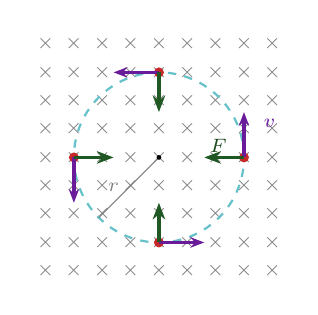
\begin{tikzpicture}[scale=0.72]
\xgrid{-4}{4}{-4}{4}
\draw[fieldc!60,dashed,thick] (0,0) circle (1.5);
\foreach \a in {0,90,180,270}{
  \coordinate (P) at (\a:1.5);
  \fill[emred] (P) circle (2.5pt);
  \draw[vvec] (P) -- ($(P)+(\a+90:0.8)$);
  \draw[fvec] (P) -- ($(P)+(\a+180:0.7)$);}
\node[font=\scriptsize,empurple] at (1.95,0.6) {$v$};
\node[font=\scriptsize,emgreen!60!black] at (1.05,0.2) {$F$};
\draw[gray] (0,0) -- (-1.06,-1.06) node[midway,left,font=\scriptsize]{$r$};
\fill (0,0) circle (1.2pt);
\end{tikzpicture}\\
{\scriptsize fig-E-1: $F\perp v$ always, towards the centre}
\column{0.62\textwidth}
\begin{steps}[3.6cm]
\stp1 & F=qvB & $v\perp B$, so $\sin90^\circ=1$\\
\stp2 & F\perp v & force never changes the speed, only the direction $\Rightarrow$ uniform circular motion\\
\stp3 & \frac{mv^2}{r}=qvB & magnetic force supplies the centripetal force\\
\stp4 & r=\frac{mv}{Bq} & multiply by $r$, cancel one $v$, divide by $qB$\\
\stp5 & T=\frac{2\pi r}{v} & time = circumference $\div$ speed\\
\stp6 & T=\frac{2\pi}{v}\cdot\frac{mv}{Bq}=\frac{2\pi m}{Bq} & substitute $r$; $v$ cancels\\
\end{steps}
\end{columns}
{\small\textbf{Note:} $T$ does \textbf{not} depend on speed: a faster particle moves in a bigger circle in the same time.}
\end{frame}

% =====================================================================
\begin{frame}{Solved numericals: force on a moving charge \hfill \badge{2M}}
\small
\begin{columns}[T]
\column{0.5\textwidth}
\begin{tcolorbox}[colback=emblue!4,colframe=emblue,title={\textbf{Q1.} A proton ($1.6\times10^{-19}$ C) moves at $2\times10^6$ m/s $\perp$ to $B=0.5$ T. Find $F$.}]
\stp1 $F=qvB$ \;($\theta=90^\circ$)\\
\stp2 $F=1.6\times10^{-19}\times2\times10^6\times0.5$\\
\stp3 $F=\boxed{1.6\times10^{-13}\ \text{N}}$
\end{tcolorbox}
\pause
\begin{tcolorbox}[colback=emblue!4,colframe=emblue,title={\textbf{Q2.} Same proton moves at $30^\circ$ to $B$.}]
\stp1 $F=qvB\sin30^\circ=1.6\times10^{-13}\times\frac12$\\
\stp2 $F=\boxed{8\times10^{-14}\ \text{N}}$
\end{tcolorbox}
\column{0.5\textwidth}
\pause
\begin{tcolorbox}[colback=emgreen!5,colframe=emgreen,title={\textbf{Q3.} Electron ($m=9.1\times10^{-31}$ kg) at $10^6$ m/s $\perp$ to $B=10^{-3}$ T. Radius?}]
\stp1 $r=\dfrac{mv}{Bq}=\dfrac{9.1\times10^{-31}\times10^6}{10^{-3}\times1.6\times10^{-19}}$\\[3pt]
\stp2 $=\dfrac{9.1\times10^{-25}}{1.6\times10^{-22}}=\boxed{5.7\times10^{-3}\ \text{m}}\approx5.7$ mm
\end{tcolorbox}
\pause
\begin{think}
\small A charge moves parallel to $B$. Force?\\
\onslide<5->{\textbf{Zero}, since $\sin0^\circ=0$.}
\end{think}
\end{columns}
\end{frame}

% =====================================================================
\begin{frame}[shrink=6]{Derivation 3: force on a current-carrying wire, $F=ILB$ \hfill \badge{4M}}
\begin{columns}[T]
\column{0.34\textwidth}\centering
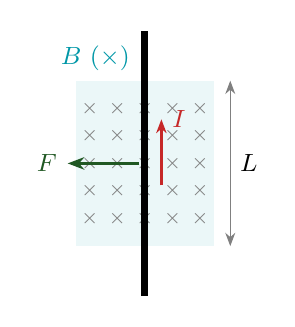
\begin{tikzpicture}[scale=0.7]
\fill[fieldc!8] (-1.25,-1.5) rectangle (1.25,1.5);
\xgrid{-2}{2}{-2}{2}
\draw[line width=2.5pt] (0,-2.4) -- (0,2.4);
\draw[cur] (0.3,-0.4) -- (0.3,0.8) node[right,font=\small]{$I$};
\draw[fvec] (-0.1,0) -- (-1.4,0) node[left,font=\small]{$F$};
\draw[{Stealth}-{Stealth},gray] (1.55,-1.5) -- (1.55,1.5) node[midway,right,font=\small,black]{$L$};
\node[font=\small,fieldc] at (-0.9,1.9) {$B\ (\times)$};
\end{tikzpicture}\\
{\scriptsize fig-9: only length $L$ lies in the field}\\[4pt]
\begin{examtip}
\scriptsize $\parallel B$: $F=0$.\; $\perp B$: $F=ILB$ (max). In fig-9 the force on the upward current is to the \textbf{left} (right hand rule).
\end{examtip}
\column{0.64\textwidth}
\begin{steps}[3.0cm]
\stp1 & F_0=qvB & force on one charge moving with drift velocity $v$ $\perp B$\\
\stp2 & F=QvB\;\cdots(1) & add up for the total charge $Q$ inside the field\\
\stp3 & t=\frac{L}{v}\Rightarrow v=\frac{L}{t}\;\cdots(2) & time for the charge to cross the length $L$\\
\stp4 & F=\frac{QLB}{t}=\frac{Q}{t}LB\;\cdots(3) & put (2) in (1)\\
\stp5 & I=\frac{Q}{t} & definition of current\\
\stp6 & F=ILB\;\cdots(4) & put step 5 in (3)\\
\stp7 & F=ILB\sin\theta\;\cdots(5) & $\theta$ = angle between current and field\\
\end{steps}
\end{columns}
\end{frame}

% =====================================================================
\begin{frame}{Activity 8: wire in a horseshoe magnet \hfill \badge{4M: experiment}}
\begin{columns}[T]
\column{0.5\textwidth}\centering
\figlab{wire_force_setup.png}{width=0.8\linewidth}{
\draw[fptr] (0.60,1.10) node[flab,anchor=south]{horseshoe magnet} -- (0.50,0.93);
\draw[fptr] (0.10,1.10) node[flab,anchor=south]{copper wire} -- (0.30,0.86);
\draw[fptr] (0.36,0.62) node[flab,anchor=east]{force $F$} -- (0.48,0.62);
\draw[fptr] (0.05,0.42) node[flab,anchor=east]{wooden stick} -- (0.23,0.45);
\draw[fptr] (0.35,0.05) node[flab,anchor=north]{9 V battery} -- (0.44,0.38);
\draw[fptr] (0.66,0.05) node[flab,anchor=north]{switch} -- (0.52,0.36);
\draw[fptr] (0.85,-0.12) node[flab,anchor=north]{wooden plank} -- (0.88,0.22);}\\[14pt]
{\scriptsize fig-10}
\column{0.46\textwidth}
\small
\begin{enumerate}
\item Stretch a copper wire between two split sticks; connect to a 9 V battery and switch.
\item Switch on and bring a horseshoe magnet around the wire.
\item The wire is \textbf{deflected}; the direction agrees with the right hand rule.
\item Reverse the magnet's poles, or reverse the current: the deflection \textbf{reverses}.
\end{enumerate}
\begin{answer}[Conclusion]
\small A current-carrying wire in a magnetic field experiences a force; its direction depends on the directions of the current and of the field.
\end{answer}
\end{columns}
\end{frame}

% =====================================================================
\begin{frame}{Why does the wire move? Combining the fields \hfill \badge{2M} \badge{4M}}
\begin{columns}[c]
\column{0.24\textwidth}\centering
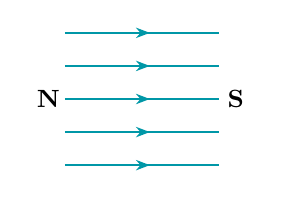
\begin{tikzpicture}[scale=0.7]
\foreach \y in {-1.2,-0.6,0,0.6,1.2} \draw[fl=0.55] (-1.4,\y) -- (1.4,\y);
\node[font=\small\bfseries] at (-1.7,0) {N}; \node[font=\small\bfseries] at (1.7,0) {S};
\end{tikzpicture}\\{\scriptsize (a) magnet's field}
\column{0.24\textwidth}\centering
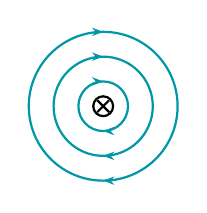
\begin{tikzpicture}[scale=0.7]
\foreach \r in {0.45,0.9,1.35} \draw[fieldc,thick,postaction={decorate},decoration={markings,mark=at position 0.25 with {\arrowreversed{Stealth[length=4pt]}},mark=at position 0.75 with {\arrowreversed{Stealth[length=4pt]}}}] (0,0) circle (\r);
\inpage{(0,0)}
\end{tikzpicture}\\{\scriptsize (b) wire, current into page (clockwise)}
\column{0.24\textwidth}\centering
\figlab{combined_field.png}{width=0.85\linewidth}{
\node[flab,anchor=south] at (0.5,1.0) {strong (fields add)};
\node[flab,anchor=north] at (0.5,0.0) {weak (fields oppose)};
\draw[fvec] (0.5,0.46) -- (0.5,0.20);}\\[8pt]{\scriptsize (c) resultant: wire pushed to weak side}
\column{0.26\textwidth}
\small
\begin{itemize}
\item Above the wire, its clockwise field points \textbf{with} the magnet's field: strong.
\item Below, it points \textbf{against}: weak.
\item The non-uniform field pushes the wire from the strong to the \textbf{weak} region.
\end{itemize}
\end{columns}
\vspace{2pt}
{\scriptsize Check with the rule: $I$ into page, $B$ left to right $\Rightarrow F$ downward. \;fig-11(a),(b),(c)}
\end{frame}

% =====================================================================
\begin{frame}{Solved numericals: force on a wire \hfill \badge{2M}}
\small
\begin{columns}[T]
\column{0.5\textwidth}
\begin{tcolorbox}[colback=emblue!4,colframe=emblue,title={\textbf{Textbook App.\ Q4.} $F=8$ N on a 20 cm conductor $\perp$ to $B$, $I=40$ A. Find $B$.}]
\stp1 $L=20$ cm $=0.2$ m\\
\stp2 $F=ILB\Rightarrow B=\dfrac{F}{IL}$\\[2pt]
\stp3 $B=\dfrac{8}{40\times0.2}=\dfrac{8}{8}=\boxed{1\ \text{T}}$
\end{tcolorbox}
\pause
\begin{tcolorbox}[colback=emblue!4,colframe=emblue,title={\textbf{Q2.} $I=5$ A, $L=0.5$ m, $B=0.2$ T, wire at $30^\circ$ to $B$.}]
\stp1 $F=ILB\sin30^\circ=5\times0.5\times0.2\times\frac12=\boxed{0.25\ \text{N}}$
\end{tcolorbox}
\column{0.5\textwidth}
\pause
\begin{tcolorbox}[colback=emgreen!5,colframe=emgreen,title={\textbf{Textbook App.\ Q3 (fig-Q5).} Wire along its length, current $i$ upward, $B$ into page, length $L$ in field.}]
\begin{minipage}{0.3\linewidth}\centering
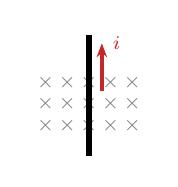
\begin{tikzpicture}[scale=0.55]
\xgrid{-2}{2}{-1}{1}
\draw[line width=2pt] (0,-1.2) -- (0,1.6);
\draw[cur] (0.3,0.3) -- (0.3,1.4) node[right,font=\scriptsize]{$i$};
\end{tikzpicture}
\end{minipage}\hfill
\begin{minipage}{0.66\linewidth}
\stp1 $\theta=90^\circ\Rightarrow F=iLB$\\
\stp2 Right hand rule: forefinger up ($i$), middle finger into page ($B$) $\Rightarrow$ thumb points \textbf{to the left}.
\end{minipage}
\end{tcolorbox}
\pause
\begin{think}
\small Force on a wire kept \textbf{parallel} to $B$?\\
\onslide<5->{\textbf{Zero}: every charge moves along the field.}
\end{think}
\end{columns}
\end{frame}

% =====================================================================
\begin{frame}{Motor in simple words}
\begin{simple}[Three ideas, in order]
\begin{enumerate}
\item A wire carrying current inside a magnetic field gets \textbf{pushed} sideways.
\item A coil has two long sides with currents in \textbf{opposite} directions, so one side is pushed \textbf{up} and the other \textbf{down}: the coil \textbf{spins}.
\item After half a turn the pushes would stop the spin. The \textbf{split ring (commutator)} reverses the current at that moment, so the coil keeps turning the same way.
\end{enumerate}
\end{simple}
\begin{examtip}[Pedal analogy]
Cycling: push down with one foot, then the other. The commutator is you switching feet at exactly the right time.
\end{examtip}
\end{frame}

% =====================================================================
\begin{frame}[shrink=6]{10.4.1 Electric motor: forces on a coil \hfill \badge{4M}}
\begin{columns}[c]
\column{0.44\textwidth}\centering
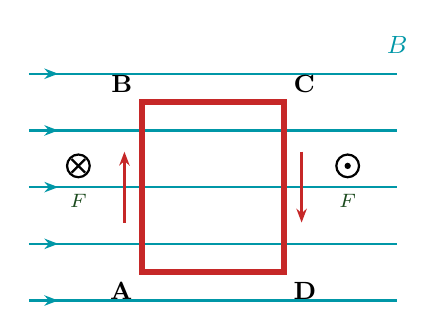
\begin{tikzpicture}[scale=0.9]
\foreach \y in {-1.6,-0.8,0,0.8,1.6} \draw[fl=0.08] (-2.6,\y) -- (2.6,\y);
\node[font=\small\bfseries,fieldc] at (2.6,2.0) {$B$};
\coordinate (A) at (-1,-1.2); \coordinate (Bc) at (-1,1.2); \coordinate (C) at (1,1.2); \coordinate (D) at (1,-1.2);
\draw[emred,line width=2pt] (A) -- (Bc) -- (C) -- (D) -- cycle;
\draw[cur] (-1.25,-0.5) -- (-1.25,0.5); \draw[cur] (1.25,0.5) -- (1.25,-0.5);
\node[below left,font=\small\bfseries] at (A) {A}; \node[above left,font=\small\bfseries] at (Bc) {B};
\node[above right,font=\small\bfseries] at (C) {C}; \node[below right,font=\small\bfseries] at (D) {D};
\inpage[0.16]{(-1.9,0.3)} \node[font=\scriptsize,emgreen!60!black] at (-1.9,-0.2) {$F$};
\outpage[0.16]{(1.9,0.3)} \node[font=\scriptsize,emgreen!60!black] at (1.9,-0.2) {$F$};
\end{tikzpicture}\\
{\scriptsize fig-12(a): current A$\to$B$\to$C$\to$D; $F$ on AB into page, on CD out of page}
\column{0.54\textwidth}
\small
\begin{enumerate}
\item AB and CD are always \textbf{perpendicular} to $B$ $\Rightarrow$ force $ILB$ on each.
\item Right hand rule: on AB (current up) force \textbf{into} the page; on CD (current down) force \textbf{out of} the page.
\item BC and DA: force zero when parallel to $B$; otherwise equal and opposite (up on BC, down on DA).
\item Forces on AB and CD: equal, opposite (equal currents in opposite directions) $\Rightarrow$ \imp{net force = 0}.
\item But they act along \textbf{different lines} $\Rightarrow$ they form a \key{couple} and \textbf{rotate} the coil, like two hands opening a bottle cap.
\end{enumerate}
\end{columns}
\end{frame}

% =====================================================================
\begin{frame}[shrink=6]{Electric motor: continuous rotation \hfill \badge{4M} \badge{Diagram}}
\begin{columns}[T]
\column{0.44\textwidth}\centering
\figlab{motor.png}{height=0.6\textheight}{
\node[font=\small\bfseries,emred] at (0.18,0.94) {N};
\node[font=\small\bfseries,emred] at (0.86,0.95) {S};
\draw[fptr] (0.55,1.05) node[flab,anchor=south]{coil ABCD, rotation axis} -- (0.58,0.84);
\draw[fptr] (-0.12,0.52) node[flab,anchor=east,align=right]{split rings\\C$_1$, C$_2$} -- (0.30,0.38);
\draw[fptr] (-0.12,0.52) -- (0.46,0.40);
\draw[fptr] (-0.12,0.30) node[flab,anchor=east,align=right]{brushes\\B$_1$, B$_2$} -- (0.12,0.37);
\draw[fptr] (-0.12,0.30) -- (0.58,0.30);
\node[font=\scriptsize\bfseries] at (0.13,0.00) {$+$};
\node[font=\scriptsize\bfseries] at (0.40,-0.02) {$-$};
\node[flab,anchor=north] at (0.27,-0.05) {battery};}\\[10pt]
{\scriptsize fig-12(c): simple electric motor}
\column{0.54\textwidth}
\footnotesize
\begin{itemize}
\item Without reversal: the coil turns to the vertical, overshoots by inertia, then the forces turn it \textbf{back}; it rocks to and fro.
\item \textbf{Fix:} reverse the current in the coil \textbf{every half rotation}.
\item The coil ends go to rings C$_1$, C$_2$ that rotate with it; fixed brushes B$_1$, B$_2$ connect to the battery.
\item After each half turn the rings swap brushes $\Rightarrow$ current in the coil reverses $\Rightarrow$ rotation continues in the \textbf{same direction}.
\end{itemize}
\begin{answer}[Energy]
\small Motor: \imp{electrical energy $\to$ mechanical energy}.
\end{answer}
\begin{tcolorbox}[colback=emteal!6,colframe=emteal,title={\textbf{Do you know? Fleming's left hand rule}}]
\scriptsize Stretch left-hand thumb, forefinger and middle finger mutually perpendicular: \textbf{forefinger} = field, \textbf{middle finger} = current, \textbf{thumb} = force (motion).
\end{tcolorbox}
\end{columns}
\end{frame}

% =====================================================================
\section{Part C: Electromagnetic induction}
% =====================================================================
\begin{frame}{Part C: Changing fields make currents}
\begin{goals}
\large\begin{itemize}
\item Explain \textbf{electromagnetic induction} with the magnet-and-coil activity.
\item State \textbf{Faraday's law} and \textbf{Lenz's law} and apply them.
\item Derive the motional emf $\varepsilon=Blv$.
\item Explain how \textbf{AC and DC generators} and magnetic levitation work.
\end{itemize}
\end{goals}
\end{frame}

\begin{frame}[shrink=6]{10.5 Electromagnetic induction (Activity 9) \hfill \badge{2M} \badge{4M}}
\begin{columns}[T]
\column{0.44\textwidth}\centering
\figlab{induction_setup.png}{width=0.82\linewidth}{
\node[font=\small\bfseries,emred] at (0.50,0.67) {N};
\draw[fptr] (0.62,1.08) node[flab,anchor=south]{bar magnet pushed in} -- (0.78,0.92);
\draw[fptr] (0.10,1.00) node[flab,anchor=south]{coil} -- (0.27,0.80);
\draw[fptr] (0.30,-0.08) node[flab,anchor=north]{galvanometer G} -- (0.11,0.07);}\\[12pt]
{\scriptsize fig-13}
\column{0.54\textwidth}
\footnotesize
\renewcommand{\arraystretch}{1.0}
\begin{tabular}{@{}p{3.3cm}p{2.6cm}@{}}
\toprule
\textbf{What we do} & \textbf{Galvanometer}\\
\midrule
Magnet at rest near coil & no deflection\\
N pole moved \textbf{towards} coil & deflects one way\\
N pole moved \textbf{away} & deflects the \textbf{other} way\\
S pole used instead & deflections reversed\\
Coil moved, magnet fixed & also deflects\\
\bottomrule
\end{tabular}
\begin{defn}[Electromagnetic induction]
\small Producing a current in a coil by \textbf{relative motion} between the coil and a magnet (changing flux). The current is the \key{induced current}; it is driven by an \key{induced emf}.
\end{defn}
\end{columns}
\end{frame}

% =====================================================================
\begin{frame}{Induction in simple words: only \emph{change} counts}
\begin{simple}[Key idea]
A magnet sitting still inside a coil makes \textbf{no} current, however strong it is. A magnet that is \textbf{moving} (or a field that is changing) makes a current.
\end{simple}
\begin{itemize}
\item \textbf{Faster} movement $\Rightarrow$ \textbf{larger} induced emf.
\item \textbf{More turns} in the coil $\Rightarrow$ larger induced emf.
\item \textbf{Stronger} magnet $\Rightarrow$ larger induced emf.
\item Reverse the motion $\Rightarrow$ the current flows the \textbf{opposite} way.
\end{itemize}
\end{frame}

% =====================================================================
\begin{frame}{10.5.1 Faraday's law \hfill \badge{1M} \badge{2M} \badge{4M}}
\begin{columns}[T]
\column{0.55\textwidth}
\begin{defn}[Faraday's law (first form)]
\small Whenever there is a \textbf{continuous change of magnetic flux} linked with a closed coil, a current is generated in the coil.
\end{defn}
\begin{defn}[Faraday's law of induction]
\small The induced emf in a closed loop \textbf{equals the rate of change of magnetic flux} through it.
\end{defn}
\small Faster change of flux $\Rightarrow$ greater induced emf.
\column{0.43\textwidth}
\begin{formula}
\[\varepsilon=\frac{\Delta\Phi}{\Delta t}\;\cdots(6)\]
Coil of $N$ turns, flux $\Phi_0$ per turn:
\[\Phi=N\Phi_0\;\cdots(7)\qquad\varepsilon=N\frac{\Delta\Phi_0}{\Delta t}\]
\end{formula}
\begin{examtip}
\small No change of flux $\Rightarrow$ no emf, however strong the field.
\end{examtip}
\end{columns}
\end{frame}

% =====================================================================
\begin{frame}{Lenz's law in simple words: nature resists change}
\begin{simple}[Think of a heavy door]
Push a heavy door and you \textbf{feel it push back}. The coil does the same: when you push a magnet in, the induced current makes the coil push \textbf{back}.
\end{simple}
\begin{itemize}
\item Induced current \textbf{always opposes} what causes it.
\item Magnet approaching $\Rightarrow$ coil face becomes the \textbf{same pole} (repels).
\item Magnet leaving $\Rightarrow$ coil face becomes the \textbf{opposite} pole (attracts).
\end{itemize}
\begin{examtip}[Why must it oppose?]
If it helped the motion, the magnet would speed up by itself and give free energy forever. That breaks \textbf{conservation of energy}.
\end{examtip}
\end{frame}

% =====================================================================
\begin{frame}{10.5.2 Lenz's law: the direction of the induced current \hfill \badge{2M} \badge{4M}}
\begin{columns}[T]
\column{0.44\textwidth}\centering
\figlab{lenz.png}{width=0.95\linewidth}{
\node[font=\small\bfseries,emred] at (0.44,0.50) {N};
\node[font=\small\bfseries,emred] at (0.97,0.50) {S};
\draw[fptr] (0.36,1.08) node[flab,anchor=south]{coil face near magnet becomes N} -- (0.20,0.86);
\draw[fptr] (0.62,0.08) node[flab,anchor=north]{magnet pushed towards coil} -- (0.55,0.33);
\node[flab,anchor=east] at (0.14,0.52) {coil};}\\[12pt]
{\scriptsize fig-14: N faces N $\Rightarrow$ the coil repels the magnet}
\column{0.54\textwidth}
\small
\textbf{Reasoning (conservation of energy):}
\begin{enumerate}
\item Suppose the induced current made the coil's near face \textbf{S}. It would \textbf{attract} the approaching N pole; the magnet would speed up and gain kinetic energy \textbf{from nothing}, and electrical energy would also appear. Impossible.
\item So the near face must be \textbf{N}: it \textbf{repels} the magnet. We must do work to push it; that work becomes electrical energy.
\item Pulling the magnet away: the near face becomes \textbf{S} and attracts, again opposing the motion.
\end{enumerate}
\begin{defn}[Lenz's law]
\small The induced current flows in a direction that \textbf{opposes the change in flux} that produces it.
\end{defn}
\end{columns}
\end{frame}

% =====================================================================
\begin{frame}[shrink=6]{10.5.3 Derivation 4, part 1: the set-up \hfill \badge{4M}}
\begin{columns}[T]
\column{0.5\textwidth}\centering
\figlab{crosswire.png}{width=0.95\linewidth}{
\node[font=\small\bfseries,emred] at (0.36,0.93) {N};
\node[font=\small\bfseries,emred] at (0.36,0.38) {S};
\draw[fptr] (0.55,1.07) node[flab,anchor=south]{distance $s$} -- (0.64,0.85);
\node[flab] at (0.975,0.53) {$l$};
\draw[fptr] (0.97,1.07) node[flab,anchor=south]{parallel conductors} -- (0.88,0.68);
\draw[fptr] (0.70,0.12) node[flab,anchor=north]{cross wire} -- (0.50,0.62);
\draw[fptr] (0.08,0.98) node[flab,anchor=south]{induced current} -- (0.10,0.72);
\draw[fptr] (0.05,0.05) node[flab,anchor=north]{galvanometer} -- (0.10,0.30);
\node[flab] at (0.45,0.52) {$B$ (downwards)};}\\[10pt]
{\scriptsize fig-15}
\column{0.48\textwidth}
\small
\begin{itemize}
\item Two parallel bare conductors, $l$ metres apart, in a uniform field $B$ (perpendicular to their plane), joined through a galvanometer.
\item A bare \textbf{cross wire} rests across them, closing the loop.
\item Move the cross wire to the \textbf{left}: needle deflects one way. To the \textbf{right}: the other way.
\item It moves a distance $s$ in time $\Delta t$, with speed $v=\dfrac{s}{\Delta t}$.
\item A current $I$ flows $\Rightarrow$ there is an emf $\varepsilon$. By \textbf{conservation of energy}, the electrical energy comes from the work we do in moving the wire (friction ignored).
\end{itemize}
\end{columns}
\end{frame}

\begin{frame}[shrink=6]{Derivation 4, part 2: work done equals flux change $\times$ current \hfill \badge{4M}}
\begin{columns}[T]
\column{0.33\textwidth}\centering
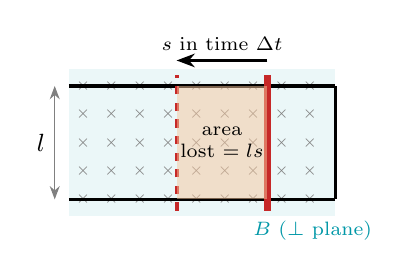
\begin{tikzpicture}[scale=0.72]
\fill[fieldc!8] (-0.5,-0.3) rectangle (4.2,2.3);
\foreach \x in {0,...,8}{\foreach \y in {0,...,4}{\node[font=\tiny,gray] at (\x*0.5-0.25,\y*0.5) {$\times$};}}
\draw[very thick] (-0.5,0) -- (4.2,0); \draw[very thick] (-0.5,2) -- (4.2,2);
\draw[very thick] (4.2,0) -- (4.2,2);
\draw[emred,line width=2.5pt] (3,-0.2) -- (3,2.2);
\draw[emred,dashed,line width=1.5pt] (1.4,-0.2) -- (1.4,2.2);
\draw[-{Stealth},thick] (3,2.45) -- (1.4,2.45) node[midway,above,font=\scriptsize]{$s$ in time $\Delta t$};
\draw[{Stealth}-{Stealth},gray] (-0.75,0) -- (-0.75,2) node[midway,left,font=\small,black]{$l$};
\fill[emorange!40,opacity=0.5] (1.4,0) rectangle (3,2);
\node[font=\scriptsize,align=center] at (2.2,1) {area\\lost $=ls$};
\node[font=\scriptsize,fieldc] at (3.8,-0.55) {$B$ ($\perp$ plane)};
\end{tikzpicture}\\
{\scriptsize top view of the loop}
\column{0.66\textwidth}
\begin{steps}[5.2cm]
\stp1 & F=BIl\;\cdots(8) & field's force on current $I$ in length $l$ (eq.\ 4); opposes our push\\
\stp2 & W=Fs=BIls\;\cdots(9) & our work against it over distance $s$\\
\stp3 & \Delta\Phi=B\,(ls)\;\cdots(10) & loop area falls by $ls$; $B\perp$ area so $\Phi=BA$\\
\stp4 & W=(\Delta\Phi)\,I & compare (9) and (10): $Bls=\Delta\Phi$\\
\stp5 & \frac{W}{\Delta t}=\frac{I\,\Delta\Phi}{\Delta t}\;\cdots(11) & divide by $\Delta t$ (work per second)\\
\stp6 & P=\varepsilon I\;\cdots(12) & electric power = emf $\times$ current\\
\stp7 & \varepsilon=\frac{\Delta\Phi}{\Delta t} & compare (11), (12): \textbf{Faraday's law}\\
\end{steps}
\end{columns}
\end{frame}

\begin{frame}[shrink=6]{Derivation 4, part 3: motional emf, $\varepsilon=Blv$ \hfill \badge{4M}}
\begin{columns}[T]
\column{0.6\textwidth}
\begin{steps}[3.1cm]
\stp1 & \frac{W}{\Delta t}=\frac{Fs}{\Delta t}=\frac{BIls}{\Delta t}\;\cdots(13) & divide (9) by $\Delta t$\\
\stp2 & \frac{s}{\Delta t}=v & speed of the cross wire\\
\stp3 & P=Fv=BIlv\;\cdots(14) & power = force $\times$ velocity\\
\stp4 & \varepsilon I=BIlv & (12) and (14) are the same power\\
\stp5 & \varepsilon=Blv & cancel $I$ on both sides\\
\end{steps}
\begin{formula}[Motional emf]
\[\boxed{\varepsilon=Blv}\]
emf between the ends of a conductor of length $l$ moving with speed $v$ perpendicular to a uniform field $B$.
\end{formula}
\column{0.38\textwidth}
\begin{examtip}[Note]
\small $\varepsilon=Blv$ is \textbf{not} Faraday's law itself: it refers to a \textbf{single moving conductor}, not a loop. It is useful whenever a conductor moves in a uniform field.
\end{examtip}
\begin{tcolorbox}[colback=emblue!5,colframe=emblue,title={\textbf{Chain of equations}}]
\scriptsize (8) $F=BIl$ $\to$ (9) $W=BIls$\\
(10) $\Delta\Phi=Bls$ $\to$ $W=I\Delta\Phi$\\
(11) $\div\Delta t$, (12) $P=\varepsilon I$ $\to$ $\varepsilon=\frac{\Delta\Phi}{\Delta t}$\\
(13), (14) $P=Fv=BIlv$ $\to$ $\varepsilon=Blv$
\end{tcolorbox}
\end{columns}
\end{frame}

% =====================================================================
\begin{frame}[shrink=6]{Solved examples: induced emf \hfill \badge{2M} \badge{4M}}
\small
\begin{columns}[T]
\column{0.52\textwidth}
\begin{tcolorbox}[colback=emblue!4,colframe=emblue,title={\textbf{Example 1 (textbook).} Coil of 400 turns; flux per turn varies as in the graph.}]
\centering
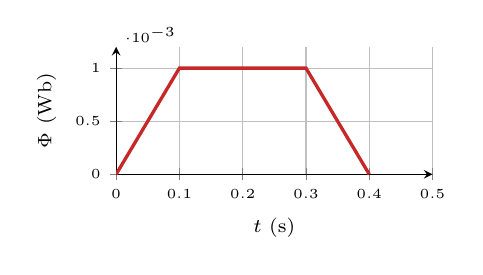
\begin{tikzpicture}
\begin{axis}[width=5.6cm,height=3.2cm,axis lines=left,xmin=0,xmax=0.5,ymin=0,ymax=0.0012,
  xtick={0,0.1,0.2,0.3,0.4,0.5},ytick={0,0.0005,0.001},
  yticklabel style={/pgf/number format/fixed,/pgf/number format/precision=4,font=\tiny},
  xticklabel style={font=\tiny},xlabel={\scriptsize $t$ (s)},ylabel={\scriptsize $\Phi$ (Wb)},grid=major]
\addplot[emred,very thick] coordinates {(0,0)(0.1,0.001)(0.3,0.001)(0.4,0)};
\end{axis}
\end{tikzpicture}\\[-2pt]
\raggedright
\stp1 0 to 0.1 s: $\Delta\Phi_0=0.001$ Wb, $\Delta t=0.1$ s\\
\stp2 $\varepsilon=N\dfrac{\Delta\Phi_0}{\Delta t}=\dfrac{400\times0.001}{0.1}=\boxed{4\ \text{V}}$ (maximum)\\
\stp3 0.1 s to 0.3 s: flux constant $\Rightarrow\Delta\Phi=0\Rightarrow\varepsilon=\boxed{0}$
\end{tcolorbox}
\column{0.46\textwidth}
\pause
\begin{tcolorbox}[colback=emgreen!5,colframe=emgreen,title={\textbf{Example 2 (textbook).} $v=10$ m/s $\perp B=0.8$ T, $\varepsilon=8$ V. Find $l$.}]
\stp1 $\varepsilon=Blv\Rightarrow l=\dfrac{\varepsilon}{Bv}$\\[2pt]
\stp2 $l=\dfrac{8}{0.8\times10}=\boxed{1\ \text{m}}$
\end{tcolorbox}
\pause
\begin{tcolorbox}[colback=emblue!4,colframe=emblue,title={\textbf{Q3.} Flux through a 50-turn coil falls from $0.02$ Wb to 0 in $0.1$ s (per turn).}]
\stp1 $\varepsilon=N\dfrac{\Delta\Phi_0}{\Delta t}=\dfrac{50\times0.02}{0.1}=\boxed{10\ \text{V}}$
\end{tcolorbox}
\end{columns}
\end{frame}

% =====================================================================
\begin{frame}{10.5.4 Applications of electromagnetic induction \hfill \badge{2M} \badge{Textbook App.\ Q6}}
\begin{columns}[T]
\column{0.5\textwidth}
\begin{tcolorbox}[colback=emblue!5,colframe=emblue,title={\textbf{Security check (metal detector)}}]
\small People walk through a large coil carrying a weak AC field. Iron on the body changes the flux linked with the coil; the induced current \textbf{triggers an alarm}.
\end{tcolorbox}
\begin{tcolorbox}[colback=emblue!5,colframe=emblue,title={\textbf{Tape recorder}}]
\small Tape coated with iron oxide is magnetised unevenly. Moving past a small coil (the head), its changing field induces a current in the coil.
\end{tcolorbox}
\column{0.48\textwidth}
\begin{tcolorbox}[colback=emgreen!5,colframe=emgreen,title={\textbf{Induction stove}}]
\small A coil below the cooking surface carries AC $\Rightarrow$ alternating field. It induces an emf and current in the \textbf{metal pan}; the pan's resistance turns the current into \textbf{heat}, which heats the water.
\end{tcolorbox}
\begin{tcolorbox}[colback=emgreen!5,colframe=emgreen,title={\textbf{ATM card swipe}}]
\small The magnetic strip moves past a coil in the reader; the changing flux induces a current pattern that is read as the card's data.
\end{tcolorbox}
\end{columns}
\end{frame}

% =====================================================================
\begin{frame}{10.5.5 Magnetic levitation \hfill \badge{2M} \badge{4M}}
\begin{columns}[T]
\column{0.28\textwidth}\centering
\figlab{levitation.png}{height=0.55\textheight}{
\draw[fptr] (-0.15,1.02) node[flab,anchor=south west]{soft iron core} -- (0.40,0.95);
\draw[fptr] (-0.15,0.74) node[flab,anchor=east]{metal ring} -- (0.10,0.72);
\draw[fptr] (-0.15,0.50) node[flab,anchor=east]{coil} -- (0.22,0.50);
\draw[fptr] (0.80,-0.04) node[flab,anchor=north]{to AC supply} -- (0.93,0.29);
\draw[fptr] (-0.15,0.10) node[flab,anchor=east]{wooden base} -- (0.15,0.14);}\\
{\scriptsize fig-16(a)}
\column{0.24\textwidth}\centering
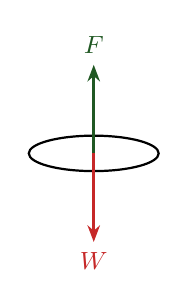
\begin{tikzpicture}[scale=0.75]
\draw[thick] (0,0) ellipse (1.1 and 0.3);
\draw[fvec] (0,0) -- (0,1.5) node[above,font=\small]{$F$};
\draw[-{Stealth[length=6pt]},emred,very thick] (0,0) -- (0,-1.5) node[below,font=\small]{$W$};
\end{tikzpicture}\\
{\scriptsize fig-16(b): $F=W$}
\column{0.46\textwidth}
\small
\begin{enumerate}
\item AC through the coil: the ring \textbf{floats}. Switch off: the ring jumps up.
\item Ring at rest $\Rightarrow$ net force 0 (Newton's 2nd law): an upward force $F$ balances the weight $W$.
\item AC keeps reversing $\Rightarrow$ the coil's poles reverse $\Rightarrow$ the flux through the ring keeps changing $\Rightarrow$ induced current in the ring.
\item By Lenz's law the ring's face is \textbf{like} the coil's top face (coil top S, ring bottom S) $\Rightarrow$ \textbf{repulsion} lifts the ring.
\item With \textbf{DC} the ring jumps only at switch on/off (flux changes only then) and falls back.
\end{enumerate}
\end{columns}
\end{frame}

\begin{frame}[shrink=8]{Levitation: why is the ring repelled? \hfill \badge{2M}}
\begin{columns}[c]
\column{0.46\textwidth}\centering
\figlab{levitation_field.png}{width=0.9\linewidth}{
\draw[fptr] (0.80,0.93) node[flab]{ring (induced current)} -- (0.80,0.66);
\draw[fptr] (0.45,0.30) node[flab]{coil} -- (0.63,0.25);
\draw[fptr] (0.12,0.62) node[flab,anchor=south]{AC source} -- (0.13,0.37);
\node[flab] at (0.30,0.93) {field lines of coil};}\\[4pt]
{\scriptsize fig-16(c)}
\column{0.52\textwidth}
\small
\begin{steps}[3.2cm]
\stp1 & \text{AC in coil} & current changes size and direction continuously\\
\stp2 & \text{flux through ring changes} & ring area fixed, field through it changes\\
\stp3 & \text{induced current in ring} & Faraday's law\\
\stp4 & \text{ring opposes the change} & Lenz's law: ring's lower face is like the coil's upper face\\
\stp5 & \text{repulsion}=W & upward force balances weight: ring floats\\
\end{steps}
\end{columns}
\end{frame}

% =====================================================================
\begin{frame}{Generator in simple words: a motor run backwards}
\begin{columns}[c]
\column{0.48\textwidth}
\begin{tcolorbox}[colback=emorange!8,colframe=emorange,title={\faCog\ Motor}]
\centering \textbf{Electrical energy} $\longrightarrow$ \textbf{motion}\\ current pushes the coil
\end{tcolorbox}
\column{0.48\textwidth}
\begin{tcolorbox}[colback=emgreen!8,colframe=emgreen,title={\faBolt\ Generator}]
\centering \textbf{Motion} $\longrightarrow$ \textbf{electrical energy}\\ we spin the coil, current appears
\end{tcolorbox}
\end{columns}
\begin{simple}[Why it works]
Spinning the coil in a magnetic field keeps changing the flux through it, so an emf is induced (Faraday's law). Turn faster $\Rightarrow$ more emf.
\end{simple}
\end{frame}

% =====================================================================
\begin{frame}{10.5.6 AC generator \hfill \badge{4M} \badge{Diagram}}
\begin{columns}[T]
\column{0.38\textwidth}\centering
\figlab{ac_generator.png}{height=0.7\textheight}{
\node[font=\small\bfseries,emred] at (0.09,0.36) {N};
\node[font=\small\bfseries,emred] at (0.91,0.50) {S};
\draw[fptr] (0.55,1.06) node[flab,anchor=south]{rotation} -- (0.48,0.93);
\draw[fptr] (-0.08,0.80) node[flab,anchor=east]{coil (side A)} -- (0.62,0.66);
\draw[fptr] (-0.08,0.60) node[flab,anchor=east]{side B} -- (0.33,0.53);
\draw[fptr] (-0.08,0.35) node[flab,anchor=east]{slip rings} -- (0.60,0.28);
\draw[fptr] (1.08,0.05) node[flab,anchor=west]{brushes} -- (0.60,0.08);
\draw[fptr] (-0.08,0.15) node[flab,anchor=east]{load} -- (0.20,0.12);}\\
{\scriptsize fig-17(a)}
\column{0.6\textwidth}
\small
\begin{itemize}
\item A coil is rotated between the poles of a magnet; the \textbf{flux through it changes} continuously $\Rightarrow$ induced emf (Faraday).
\item Coil ends go to two \textbf{full slip rings}; carbon brushes press on them and take current to the load.
\end{itemize}
\centering
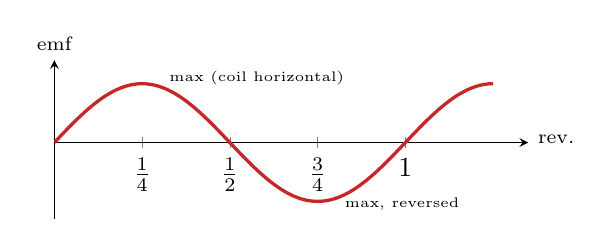
\begin{tikzpicture}
\begin{axis}[width=7.6cm,height=3.6cm,axis lines=middle,xmin=0,xmax=1.35,ymin=-1.3,ymax=1.4,
  xtick={0.25,0.5,0.75,1},xticklabels={$\frac14$,$\frac12$,$\frac34$,1},ytick=\empty,
  xlabel={\scriptsize rev.},ylabel={\scriptsize emf},every axis x label/.style={at={(1,0.5)},anchor=west},every axis y label/.style={at={(0,1)},anchor=south}]
\addplot[emred,very thick,domain=0:1.25,samples=100] {sin(deg(2*pi*x))};
\node[font=\tiny,anchor=west] at (axis cs:0.30,1.1) {max (coil horizontal)};
\node[font=\tiny,anchor=west] at (axis cs:0.80,-1.05) {max, reversed};
\end{axis}
\end{tikzpicture}\\
{\scriptsize fig-17(b): alternating emf over one rotation}
\end{columns}
\end{frame}

\begin{frame}[shrink=6]{Why does the emf vary? AC and the DC generator \hfill \badge{2M} \badge{4M}}
\begin{columns}[T]
\column{0.5\textwidth}
\small
\textbf{One rotation, step by step:}
\begin{enumerate}
\item Coil \textbf{vertical} (plane $\perp$ field): flux maximum but changing slowest $\Rightarrow$ \textbf{emf zero}.
\item First quarter: emf rises; coil \textbf{horizontal} (plane $\parallel$ field): flux changing fastest $\Rightarrow$ \textbf{emf maximum}.
\item Second quarter: emf falls to zero (vertical again, B on top).
\item Second half: same pattern but sides A and B have swapped places $\Rightarrow$ \textbf{emf reversed}.
\end{enumerate}
\begin{defn}[Alternating current (AC)]
\small Current whose direction reverses periodically; it has a \textbf{frequency}.
\end{defn}
{\small Generator: \imp{mechanical $\to$ electrical energy}.}
\column{0.48\textwidth}\centering
\figlab{dc_generator.png}{height=0.38\textheight}{
\node[font=\small\bfseries,emred] at (0.09,0.36) {N};
\node[font=\small\bfseries,emred] at (0.92,0.50) {S};
\draw[fptr] (1.08,0.38) node[flab,anchor=west,align=left]{split rings\\(commutator)} -- (0.66,0.28);
\draw[fptr] (0.20,0.10) node[flab,anchor=east]{brush} -- (0.46,0.22);
\draw[fptr] (1.08,0.05) node[flab,anchor=west]{load $R$} -- (0.80,0.08);}\\
{\scriptsize fig-17(c): DC generator}\\[2pt]
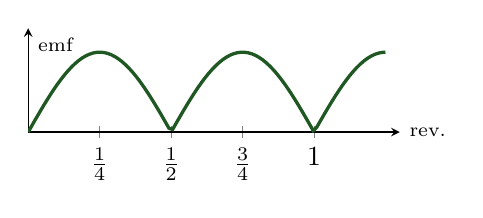
\begin{tikzpicture}
\begin{axis}[width=6.3cm,height=2.9cm,axis lines=middle,xmin=0,xmax=1.3,ymin=0,ymax=1.3,
  xtick={0.25,0.5,0.75,1},xticklabels={$\frac14$,$\frac12$,$\frac34$,1},ytick=\empty,
  xlabel={\scriptsize rev.},ylabel={\scriptsize emf},every axis x label/.style={at={(1,0)},anchor=west}]
\addplot[emgreen!70!black,very thick,domain=0:1.25,samples=100] {abs(sin(deg(2*pi*x)))};
\end{axis}
\end{tikzpicture}\\
{\scriptsize fig-17(d): with half slip rings the current in the load keeps one direction (DC)}
\end{columns}
\end{frame}

\begin{frame}{Motor vs generator \hfill \badge{2M}}
\centering\small
\renewcommand{\arraystretch}{1.45}
\begin{tabular}{>{\bfseries}p{3.2cm}p{4.9cm}p{4.9cm}}
\toprule
\rowcolor{emblue}\textcolor{white}{Feature} & \textcolor{white}{\textbf{Electric motor}} & \textcolor{white}{\textbf{Generator (dynamo)}}\\
\midrule
Energy change & electrical $\to$ mechanical & mechanical $\to$ electrical\\
Principle & force on a current-carrying coil in a field ($F=ILB$) & electromagnetic induction ($\varepsilon=\Delta\Phi/\Delta t$)\\
Input & current from a battery/supply & rotation of the coil\\
Output & rotation & induced current\\
Rings & split rings: reverse current every half turn & AC: full slip rings;\; DC: split rings\\
Hand rule & right hand rule / Fleming's left hand rule & Lenz's law gives the current direction\\
\bottomrule
\end{tabular}
\end{frame}

% =====================================================================
\section{Revision}

\begin{frame}{All derivations of this chapter at a glance \hfill \badge{Revise}}
\small\centering
\renewcommand{\arraystretch}{1.5}
\begin{tabular}{>{\bfseries}c p{3.8cm} p{5.3cm} p{2.8cm}}
\toprule
\rowcolor{emblue}\textcolor{white}{No.} & \textcolor{white}{\textbf{Result}} & \textcolor{white}{\textbf{Key idea}} & \textcolor{white}{\textbf{Uses}}\\
\midrule
1 & $\Phi=BA\cos\theta$ & effective area $\perp$ field is $A\cos\theta$ & $B=\Phi/A$\\
2 & $r=\frac{mv}{Bq}$,\; $T=\frac{2\pi m}{Bq}$ & magnetic force = centripetal force & $F=qvB$\\
3 & $F=ILB\sin\theta$ & add $qvB$ over all charges, $v=L/t$, $I=Q/t$ & $F=qvB$\\
4 & $\varepsilon=\frac{\Delta\Phi}{\Delta t}$,\; $\varepsilon=Blv$ & work done = electrical energy; $\Delta\Phi=Bls$; $P=\varepsilon I=Fv$ & $F=BIl$\\
\bottomrule
\end{tabular}
\end{frame}

\begin{frame}{Concept map}
\centering
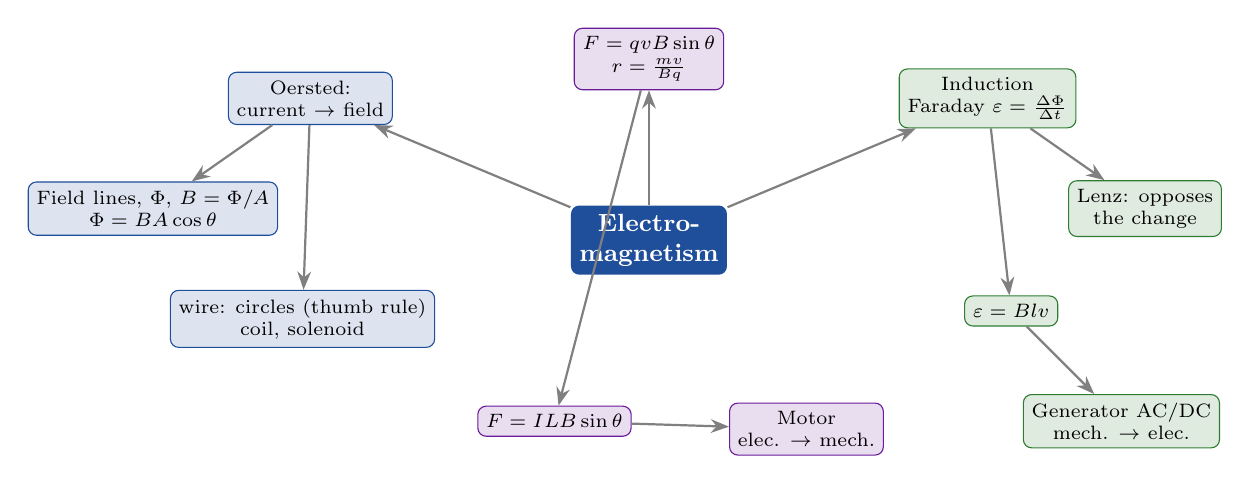
\begin{tikzpicture}[
  every node/.style={font=\scriptsize,align=center,rounded corners=3pt,inner sep=3pt},
  main/.style={fill=emblue,text=white,font=\small\bfseries},
  a/.style={fill=emblue!15,draw=emblue},
  b/.style={fill=empurple!15,draw=empurple},
  c/.style={fill=emgreen!15,draw=emgreen},
  l/.style={-{Stealth},thick,gray}]
\node[main] (c) at (0,0) {Electro-\\magnetism};
\node[a] (o) at (-4.3,1.8) {Oersted:\\current $\to$ field};
\node[a] (f) at (-6.3,0.4) {Field lines, $\Phi$, $B=\Phi/A$\\$\Phi=BA\cos\theta$};
\node[a] (w) at (-4.4,-1.0) {wire: circles (thumb rule)\\coil, solenoid};
\node[b] (q) at (0,2.3) {$F=qvB\sin\theta$\\$r=\frac{mv}{Bq}$};
\node[b] (i) at (-1.2,-2.3) {$F=ILB\sin\theta$};
\node[b] (m) at (2.0,-2.4) {Motor\\elec. $\to$ mech.};
\node[c] (e) at (4.3,1.8) {Induction\\Faraday $\varepsilon=\frac{\Delta\Phi}{\Delta t}$};
\node[c] (lz) at (6.3,0.4) {Lenz: opposes\\the change};
\node[c] (bl) at (4.6,-0.9) {$\varepsilon=Blv$};
\node[c] (g) at (6.0,-2.3) {Generator AC/DC\\mech. $\to$ elec.};
\draw[l] (c)--(o); \draw[l] (o)--(f); \draw[l] (o)--(w); \draw[l] (c)--(q); \draw[l] (q)--(i); \draw[l] (i)--(m);
\draw[l] (c)--(e); \draw[l] (e)--(lz); \draw[l] (e)--(bl); \draw[l] (bl)--(g);
\end{tikzpicture}
\end{frame}

\begin{frame}{Formula sheet \hfill \badge{Must memorise}}
\small
\renewcommand{\arraystretch}{1.55}
\centering
\begin{tabular}{>{\bfseries}p{4.8cm}p{8cm}}
\toprule
\rowcolor{emred}\textcolor{white}{Quantity} & \textcolor{white}{\textbf{Formula / unit}}\\
\midrule
Magnetic flux density & $B=\dfrac{\Phi}{A}$;\quad tesla (T) = Wb/m$^2$ = N/(A m)\\
Magnetic flux & $\Phi=BA\cos\theta$;\quad weber (Wb)\\
Force on a moving charge & $F=qvB\sin\theta$ \;($=qvB$ when $v\perp B$)\\
Charge in a uniform field & $r=\dfrac{mv}{Bq}$;\quad $T=\dfrac{2\pi m}{Bq}$\\
Force on a current & $F=ILB\sin\theta$ \;($=ILB$ when $I\perp B$)\\
Faraday's law & $\varepsilon=\dfrac{\Delta\Phi}{\Delta t}$;\quad $N$ turns: $\varepsilon=N\dfrac{\Delta\Phi_0}{\Delta t}$\\
Motional emf & $\varepsilon=Blv$\\
\bottomrule
\end{tabular}
\end{frame}

\begin{frame}{What we have learnt (textbook summary)}
\small
\begin{itemize}
\item \textbf{Magnetic flux}: a measure of the number of field lines through an area.
\item \textbf{Magnetic flux density} $B$: flux through a plane perpendicular to the field $\div$ area of the plane.
\item A current-carrying wire produces a magnetic field.
\item $F=qvB\sin\theta$ and $F=ILB\sin\theta$.
\item In an electric \textbf{motor}, electrical energy is converted into mechanical energy.
\item Producing current by relative motion between a coil and a magnetic field is \textbf{electromagnetic induction}.
\item \textbf{Faraday's law}: induced emf in a closed loop = rate of change of magnetic flux through it.
\item \textbf{Lenz's law}: the induced current opposes the change in flux.
\item A conductor of length $l$ moving $\perp$ to $B$ with speed $v$ develops the \textbf{motional emf} $Blv$.
\item In \textbf{generators}, mechanical energy is converted into electrical energy.
\end{itemize}
\end{frame}

% =====================================================================
\section{Question Bank}

\begin{frame}{1-mark questions \hfill \badge{1M}}
\small
\begin{columns}[T]
\column{0.5\textwidth}
\begin{enumerate}
\item Who showed a current affects a compass? \onslide<2->{\textcolor{emgreen}{\textbf{Oersted}}}
\item SI unit of magnetic flux? \onslide<2->{\textcolor{emgreen}{\textbf{weber}}}
\item SI unit of flux density? \onslide<2->{\textcolor{emgreen}{\textbf{tesla (Wb/m$^2$)}}}
\item Shape of field lines of a straight wire? \onslide<2->{\textcolor{emgreen}{\textbf{concentric circles}}}
\item Flux through a plane parallel to $B$? \onslide<2->{\textcolor{emgreen}{\textbf{zero}}}
\item Force on a charge moving along $B$? \onslide<2->{\textcolor{emgreen}{\textbf{zero}}}
\item Device like a bar magnet made of coils? \onslide<2->{\textcolor{emgreen}{\textbf{solenoid}}}
\end{enumerate}
\column{0.5\textwidth}
\begin{enumerate}\setcounter{enumi}{7}
\item Energy change in a motor? \onslide<2->{\textcolor{emgreen}{\textbf{electrical $\to$ mechanical}}}
\item Part that reverses current in a motor? \onslide<2->{\textcolor{emgreen}{\textbf{split rings}}}
\item Law giving the direction of induced current? \onslide<2->{\textcolor{emgreen}{\textbf{Lenz's law}}}
\item Lenz's law follows from? \onslide<2->{\textcolor{emgreen}{\textbf{conservation of energy}}}
\item Formula for motional emf? \onslide<2->{\textcolor{emgreen}{\textbf{$\varepsilon=Blv$}}}
\item Stove based on induction? \onslide<2->{\textcolor{emgreen}{\textbf{induction stove}}}
\item Rings used in an AC generator? \onslide<2->{\textcolor{emgreen}{\textbf{full slip rings}}}
\end{enumerate}
\end{columns}
\end{frame}

\begin{frame}{Textbook MCQs \hfill \badge{1M}}
\small
\begin{columns}[T]
\column{0.5\textwidth}
\begin{enumerate}
\item Converts electrical energy into mechanical energy:\\ a) motor \; b) battery \; c) generator \; d) switch\\
\onslide<2->{\textcolor{emgreen}{\textbf{Answer: a}}}
\item Converts mechanical energy into electrical energy:\\ a) motor \; b) battery \; c) generator \; d) switch\\
\onslide<2->{\textcolor{emgreen}{\textbf{Answer: c}}}
\item Force on a wire placed perpendicular to a uniform field:\\ a) 0 \; b) $ILB$ \; c) $2ILB$ \; d) $ILB/2$\\
\onslide<2->{\textcolor{emgreen}{\textbf{Answer: b}} ($\sin90^\circ=1$)}
\end{enumerate}
\column{0.5\textwidth}
\begin{enumerate}\setcounter{enumi}{3}
\item One tesla =\\ a) N/C \; b) N/(A m) \; c) A/m \; d) N/(A s)\\
\onslide<3->{\textcolor{emgreen}{\textbf{Answer: b}} ($B=F/IL$)}
\item Unit of magnetic flux:\\ a) dyne \; b) oersted \; c) gauss \; d) weber\\
\onslide<3->{\textcolor{emgreen}{\textbf{Answer: d}}}
\item No force acts on a current-carrying conductor kept\\ a) parallel to the field \; b) perpendicular to the field \; c) in the field \; d) away from the field\\
\onslide<3->{\textcolor{emgreen}{\textbf{Answer: a}}}
\end{enumerate}
\end{columns}
\end{frame}

\begin{frame}{Reflections on concepts: figure questions \hfill \badge{1M} \badge{2M}}
\footnotesize
\begin{columns}[T]
\column{0.5\textwidth}
\begin{minipage}[t]{0.3\linewidth}\centering
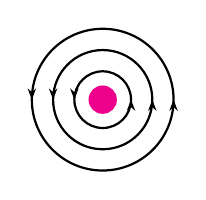
\begin{tikzpicture}[scale=0.45]
\foreach \r in {0.8,1.4,2.0} \draw[thick,postaction={decorate},decoration={markings,mark=at position 0.0 with {\arrow{Stealth[length=4pt]}},mark=at position 0.5 with {\arrow{Stealth[length=4pt]}}}] (0,0) circle (\r);
\fill[magenta] (0,0) circle (0.4);
\end{tikzpicture}\\{\tiny fig-Q1}
\end{minipage}\hfill
\begin{minipage}[t]{0.66\linewidth}
\textbf{Q2.} Field lines as in fig-Q1 (anticlockwise). Direction of current?\\
\onslide<2->{\textcolor{emgreen}{Thumb rule: anticlockwise field $\Rightarrow$ current \textbf{out of the page} (towards the reader).}}
\end{minipage}\\[6pt]
\begin{minipage}[t]{0.3\linewidth}\centering
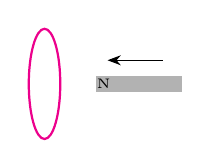
\begin{tikzpicture}[scale=0.5]
\draw[magenta,thick] (0,0) ellipse (0.4 and 1.4);
\fill[gray!60] (1.3,-0.2) rectangle (3.5,0.2); \node[font=\tiny] at (1.5,0) {N};
\draw[-{Stealth}] (3.0,0.6) -- (1.6,0.6);
\end{tikzpicture}\\{\tiny fig-Q2}
\end{minipage}\hfill
\begin{minipage}[t]{0.66\linewidth}
\textbf{Q3.} N pole moves towards the coil. What happens to the flux?\\
\onslide<3->{\textcolor{emgreen}{Flux through the coil \textbf{increases}; a current is induced so that the near face becomes N (Lenz).}}
\end{minipage}
\column{0.5\textwidth}
\begin{minipage}[t]{0.3\linewidth}\centering
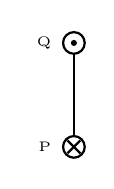
\begin{tikzpicture}[scale=0.55]
\draw[thick] (0,-1) -- (0,1);
\outpage[0.25]{(0,1.2)} \node[font=\tiny,left] at (-0.3,1.2) {Q};
\inpage[0.25]{(0,-1.2)} \node[font=\tiny,left] at (-0.3,-1.2) {P};
\end{tikzpicture}\\{\tiny fig-Q3}
\end{minipage}\hfill
\begin{minipage}[t]{0.66\linewidth}
\textbf{Q4.} Coil $\perp$ page: current into page at P, out at Q. Direction of the field of the coil?\\
\onslide<4->{\textcolor{emgreen}{Between P and Q both wires give a field to the \textbf{right}: the field is along the axis, from left to right (in the plane of the page, $\perp$ to the coil).}}
\end{minipage}\\[6pt]
\textbf{Q1.} Are field lines closed? \onslide<5->{\textcolor{emgreen}{Yes. For a straight wire they are circles; for a solenoid/bar magnet, lines outside (N $\to$ S) continue inside (S $\to$ N), forming closed loops.}}
\end{columns}
\end{frame}

\begin{frame}{Application of concepts: model answers \hfill \badge{2M}}
\footnotesize
\begin{columns}[T]
\column{0.5\textwidth}
\begin{minipage}[t]{0.22\linewidth}\centering
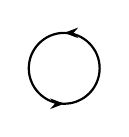
\begin{tikzpicture}[scale=0.45]
\draw[thick,postaction={decorate},decoration={markings,mark=at position 0.25 with {\arrow{Stealth[length=5pt]}},mark=at position 0.75 with {\arrow{Stealth[length=5pt]}}}] (0,0) circle (1);
\end{tikzpicture}\\{\tiny fig-Q4}
\end{minipage}\hfill
\begin{minipage}[t]{0.74\linewidth}
\textbf{1.} Current as in fig-Q4 (anticlockwise, as seen). Pole at this face?\\
\onslide<2->{\textcolor{emgreen}{\textbf{North pole}: anticlockwise current $\Rightarrow$ field points towards the viewer.}}
\end{minipage}\\[4pt]
\textbf{2.} Why is a TV picture distorted near a magnet?\\
\onslide<3->{\textcolor{emgreen}{The picture is made by a moving electron beam; the magnet's field exerts a force $F=qvB\sin\theta$ on the electrons and deflects them from their correct spots.}}\\[4pt]
\textbf{5.} Coil and magnet move in the \textbf{same direction} with the same speed (fig-Q6). What happens?\\
\onslide<4->{\textcolor{emgreen}{No relative motion $\Rightarrow$ flux through the coil does not change $\Rightarrow$ \textbf{no induced current}.}}
\column{0.5\textwidth}
\textbf{6.} Applications of Faraday's law:\\
\onslide<5->{\textcolor{emgreen}{generators, security metal detectors, tape recorder heads, induction stoves, ATM card readers, transformers.}}\\[4pt]
\textbf{Reflections Q2 of electromagnet ideas.} Why use a solenoid for an electromagnet?\\
\onslide<6->{\textcolor{emgreen}{Its field inside is strong and uniform like a bar magnet's and can be switched on/off with the current.}}\\[4pt]
\textbf{Lenz and energy.} Why is it harder to push a magnet into a closed coil than into an open one?\\
\onslide<7->{\textcolor{emgreen}{In a closed coil an induced current flows and repels the magnet; our extra work becomes electrical energy. In an open coil no current flows, so no opposing force.}}
\end{columns}
\end{frame}

\begin{frame}[shrink=6]{4-mark questions: answer points \hfill \badge{4M}}
\footnotesize
\begin{columns}[T]
\column{0.5\textwidth}
\begin{tcolorbox}[colback=emblue!4,colframe=emblue,title={\textbf{Q1. Two activities: a current-carrying wire produces a field.}}]
Activity 1 (Oersted: compass under wire deflects when switched on) $\cdot$ Activity 4 (compasses around a vertical wire set as tangents; iron filings form circles) $\cdot$ diagrams $\cdot$ conclusion.
\end{tcolorbox}
\begin{tcolorbox}[colback=emblue!4,colframe=emblue,title={\textbf{Q2. Verify the force on a wire in a field.}}]
Activity 8: wire between split sticks, 9 V battery, horseshoe magnet $\cdot$ wire deflects $\cdot$ reverse poles/current $\Rightarrow$ deflection reverses $\cdot$ right hand rule $\cdot$ $F=ILB$.
\end{tcolorbox}
\begin{tcolorbox}[colback=emblue!4,colframe=emblue,title={\textbf{Q3. Explain Faraday's law with an activity.}}]
Activity 9: coil + galvanometer, magnet in/out, at rest, S pole $\cdot$ law $\varepsilon=\Delta\Phi/\Delta t$ $\cdot$ faster motion, bigger deflection $\cdot$ $N$ turns.
\end{tcolorbox}
\column{0.5\textwidth}
\begin{tcolorbox}[colback=empurple!4,colframe=empurple,title={\textbf{Q4. Experiment for Faraday's law: instruments, tips, precautions.}}]
Coil of many turns, strong bar magnet, sensitive galvanometer, wires $\cdot$ \textbf{tips}: more turns, stronger magnet, faster motion $\cdot$ \textbf{precautions}: tight connections, galvanometer away from the magnet, note zero first, move magnet along the axis.
\end{tcolorbox}
\begin{tcolorbox}[colback=empurple!4,colframe=empurple,title={\textbf{Q5. Working of an electric motor.}}]
fig-12 $\cdot$ forces on AB, CD equal and opposite $\Rightarrow$ couple $\cdot$ split rings and brushes reverse current each half turn $\cdot$ continuous rotation $\cdot$ electrical $\to$ mechanical.
\end{tcolorbox}
\begin{tcolorbox}[colback=empurple!4,colframe=empurple,title={\textbf{Q6. Derive $\varepsilon=Blv$ / explain AC generator.}}]
Derivation 4 (eqs 8--14) \;\textbf{or}\; fig-17: rotating coil, changing flux, slip rings, emf zero/max, AC graph.
\end{tcolorbox}
\end{columns}
\end{frame}

\begin{frame}{Practice numericals (homework / class test) \hfill \badge{2M}}
\small
\begin{enumerate}
\item A flux of 0.06 Wb passes normally through 0.3 m$^2$. Find $B$. \hfill \onslide<2->{\textcolor{emgreen}{0.2 T}}
\item $B=0.4$ T, area 0.5 m$^2$, normal at $60^\circ$ to $B$. Find $\Phi$. \hfill \onslide<2->{\textcolor{emgreen}{0.1 Wb}}
\item A 2 m wire carries 3 A perpendicular to $B=0.5$ T. Find $F$. \hfill \onslide<2->{\textcolor{emgreen}{3 N}}
\item An electron ($1.6\times10^{-19}$ C) moves at $5\times10^6$ m/s $\perp B=0.2$ T. Find $F$. \hfill \onslide<2->{\textcolor{emgreen}{$1.6\times10^{-13}$ N}}
\item A 0.5 m rod moves at 4 m/s $\perp B=0.25$ T. Find the emf. \hfill \onslide<2->{\textcolor{emgreen}{0.5 V}}
\item Flux per turn in a 200-turn coil changes by $5\times10^{-3}$ Wb in 0.2 s. Find $\varepsilon$. \hfill \onslide<2->{\textcolor{emgreen}{5 V}}
\item Show that the time period of a charge in a uniform field is independent of its speed. \hfill \onslide<2->{\textcolor{emgreen}{$T=2\pi m/Bq$}}
\end{enumerate}
\end{frame}

\begin{frame}{Practice numericals: worked solutions \hfill \badge{2M}}
\footnotesize
\begin{columns}[T]
\column{0.5\textwidth}
\begin{enumerate}
\item $B=\dfrac{\Phi}{A}=\dfrac{0.06}{0.3}=\boxed{0.2\ \text{T}}$
\item $\Phi=BA\cos60^\circ=0.4\times0.5\times\frac12=\boxed{0.1\ \text{Wb}}$
\item $F=ILB=3\times2\times0.5=\boxed{3\ \text{N}}$
\item $F=qvB=1.6\times10^{-19}\times5\times10^6\times0.2$\\ $=\boxed{1.6\times10^{-13}\ \text{N}}$
\end{enumerate}
\column{0.5\textwidth}
\begin{enumerate}\setcounter{enumi}{4}
\item $\varepsilon=Blv=0.25\times0.5\times4=\boxed{0.5\ \text{V}}$
\item $\varepsilon=N\dfrac{\Delta\Phi_0}{\Delta t}=\dfrac{200\times5\times10^{-3}}{0.2}=\dfrac{1}{0.2}=\boxed{5\ \text{V}}$
\item $qvB=\dfrac{mv^2}{r}\Rightarrow r=\dfrac{mv}{Bq}$;\; $T=\dfrac{2\pi r}{v}=\dfrac{2\pi m}{Bq}$: no $v$ in the result (Derivation 2).
\end{enumerate}
\end{columns}
\end{frame}

\begin{frame}[shrink=6]{Important diagrams and common mistakes \hfill \badge{4M}}
\begin{columns}[T]
\column{0.5\textwidth}
\begin{tcolorbox}[colback=emblue!5,colframe=emblue,title={\textbf{Must practise}}]
\small
\begin{enumerate}
\item Field lines of a bar magnet -- fig-2
\item Field of a straight wire ($\odot$ and $\otimes$) -- fig-4(b),(c)
\item Field of a solenoid with N, S -- fig-6(b)
\item Right hand rule for force -- fig-8(b)
\item Coil in a field with forces -- fig-12(a); motor -- fig-12(c)
\item Faraday's activity -- fig-13;\; cross-wire set-up -- fig-15
\item AC generator and emf graph -- fig-17(a),(b)
\end{enumerate}
\end{tcolorbox}
\column{0.48\textwidth}
\begin{examtip}[Common mistakes that lose marks]
\small
\begin{itemize}
\item No arrows on field lines.
\item Using $\sin\theta$ with $\theta$ between $B$ and the \textbf{plane} instead of the \textbf{normal} in $\Phi=BA\cos\theta$.
\item Forgetting $F=0$ when the wire/charge is parallel to $B$.
\item Not reversing the force for an electron.
\item Using cm or cm$^2$ in formulas (convert to m, m$^2$).
\item Forgetting $N$ in $\varepsilon=N\,\Delta\Phi_0/\Delta t$.
\item Mixing up motor (split rings) and AC generator (slip rings).
\end{itemize}
\end{examtip}
\end{columns}
\end{frame}

\begin{frame}{Suggested experiments and projects}
\begin{columns}[T]
\column{0.5\textwidth}
\begin{activity}[Suggested experiments]
\small
\begin{enumerate}
\item Two activities showing that a current-carrying wire produces a magnetic field.
\item Verify that a current-carrying conductor experiences a force in a magnetic field.
\item Explain Faraday's law of induction with an activity.
\item Suggest an experiment for Faraday's law: instruments, tips and precautions.
\item Verify with an experiment that a current-carrying wire produces a field.
\end{enumerate}
\end{activity}
\column{0.48\textwidth}
\begin{tcolorbox}[colback=empurple!6,colframe=empurple,title={\textbf{Suggested projects}}]
\small
\begin{enumerate}
\item Collect information on generating current using Faraday's law.
\item Materials and procedure for making a simple electric motor; write a report.
\item Collect information on Faraday's experiments.
\end{enumerate}
\end{tcolorbox}
\end{columns}
\end{frame}

\begin{frame}[plain]
\begin{tikzpicture}[remember picture,overlay]
\fill[emblue] (current page.south west) rectangle (current page.north east);
\foreach \c [count=\i] in {emnavy,emblue,emteal,emgreen,emgold,emorange,emred}
  \fill[\c] ([yshift=-3.2cm-(\i-1)*0.14cm]current page.north west) rectangle ([yshift=-3.2cm-\i*0.14cm]current page.north east);
\node[white,font=\fontsize{36}{40}\selectfont\bfseries] at ([yshift=-1.8cm]current page.north) {Thank you!};
\node[white,font=\large,align=center] at ([yshift=-0.4cm]current page.center) {Keywords to revise:\\[4pt]\small magnetic flux $\cdot$ magnetic flux density $\cdot$ field lines $\cdot$ solenoid $\cdot$ electric motor $\cdot$ slip rings\\\small induced current $\cdot$ induced emf $\cdot$ Faraday's law $\cdot$ Lenz's law $\cdot$ motional emf $\cdot$ AC and DC generators};
\end{tikzpicture}
\end{frame}

\end{document}
"
\documentclass[aspectratio=169,11pt,xcolor=table]{beamer}
\usetheme{Madrid}
\usepackage[T1]{fontenc}
\usepackage{lmodern}
\usepackage{amsmath,amssymb}
\usepackage{graphicx}
\usepackage{tikz}
\usetikzlibrary{arrows.meta,calc,decorations.markings,shapes.geometric,positioning}
\usepackage{pgfplots}
\pgfplotsset{compat=1.18}
\usepackage[most]{tcolorbox}
\usepackage{booktabs,array,multicol}
\usepackage{fontawesome5}
\graphicspath{{figures/}}

% ---------------- colours ----------------
\definecolor{emblue}{HTML}{1F4E9A}
\definecolor{emteal}{HTML}{0E8C8C}
\definecolor{emorange}{HTML}{E8710A}
\definecolor{emred}{HTML}{C62828}
\definecolor{emgreen}{HTML}{2E7D32}
\definecolor{empurple}{HTML}{6A1B9A}
\definecolor{emgold}{HTML}{F9A825}
\definecolor{emnavy}{HTML}{0D2B5E}
\definecolor{fieldc}{HTML}{0097A7}

\setbeamercolor{structure}{fg=emblue}
\setbeamercolor{palette primary}{bg=emblue,fg=white}
\setbeamercolor{palette secondary}{bg=emteal,fg=white}
\setbeamercolor{palette tertiary}{bg=empurple,fg=white}
\setbeamercolor{frametitle}{bg=emblue,fg=white}
\setbeamercolor{title}{bg=emblue,fg=white}
\setbeamercolor{block title}{bg=emteal,fg=white}
\setbeamercolor{block body}{bg=emteal!8}
\setbeamertemplate{navigation symbols}{}
\tcbset{before skip=3pt,after skip=3pt,fonttitle=\bfseries\small,boxsep=2pt,left=4pt,right=4pt,top=2pt,bottom=2pt}
\setbeamertemplate{itemize item}{\color{emorange}$\blacktriangleright$}
\setbeamertemplate{itemize subitem}{\color{emteal}$\bullet$}
\setbeamertemplate{enumerate item}{\color{emblue}\bfseries\insertenumlabel.}

% ---------------- boxes ----------------
\newtcolorbox{defn}[1][Definition]{colback=emblue!6,colframe=emblue,fonttitle=\bfseries\small,
  title={\faBook\ #1},boxrule=0.8pt,arc=2mm,left=4pt,right=4pt,top=2pt,bottom=2pt}
\newtcolorbox{formula}[1][Formula]{colback=emred!5,colframe=emred,fonttitle=\bfseries\small,
  title={\faCalculator\ #1},boxrule=0.8pt,arc=2mm,left=4pt,right=4pt,top=2pt,bottom=2pt}
\newtcolorbox{examtip}[1][Exam Tip]{colback=emgold!12,colframe=emorange,fonttitle=\bfseries\small,
  title={\faStar\ #1},boxrule=0.8pt,arc=2mm,left=4pt,right=4pt,top=2pt,bottom=2pt}
\newtcolorbox{activity}[1][Activity]{colback=emgreen!6,colframe=emgreen,fonttitle=\bfseries\small,
  title={\faFlask\ #1},boxrule=0.8pt,arc=2mm,left=4pt,right=4pt,top=2pt,bottom=2pt}
\newtcolorbox{think}[1][Teacher asks]{colback=empurple!6,colframe=empurple,fonttitle=\bfseries\small,
  title={\faQuestionCircle\ #1},boxrule=0.8pt,arc=2mm,left=4pt,right=4pt,top=2pt,bottom=2pt}
\newtcolorbox{answer}[1][Answer]{colback=white,colframe=emgreen,fonttitle=\bfseries\small,
  title={\faCheckCircle\ #1},boxrule=0.8pt,arc=2mm,left=4pt,right=4pt,top=2pt,bottom=2pt}


\newtcolorbox{simple}[1][In simple words]{colback=emgold!14,colframe=emorange!85!black,fonttitle=\bfseries\small,
  title={\faLightbulb\ #1},boxrule=0.8pt,arc=2mm,left=5pt,right=5pt,top=3pt,bottom=3pt}
\newtcolorbox{goals}[1][By the end of this part you can\ldots]{colback=emgreen!6,colframe=emgreen,fonttitle=\bfseries\small,
  title={\faCheckSquare\ #1},boxrule=0.8pt,arc=2mm,left=6pt,right=6pt,top=3pt,bottom=3pt}
\tikzset{story/.style={draw=#1,fill=#1!10,very thick,rounded corners=4pt,align=center,text width=3.2cm,inner sep=5pt,font=\small}}

\newcommand{\badge}[1]{\tikz[baseline=(b.base)]\node[fill=emgold,text=black,rounded corners=3pt,
  inner sep=2.5pt,font=\scriptsize\bfseries](b){#1};}
\newcommand{\imp}[1]{\textcolor{emred}{\textbf{#1}}}
\newcommand{\key}[1]{\textcolor{emblue}{\textbf{#1}}}

% ---------------- step-by-step derivation helpers ----------------
\newcommand{\stp}[1]{\tikz[baseline=(s.base)]\node[circle,fill=emblue,text=white,inner sep=1.1pt,
  minimum size=11pt,font=\scriptsize\bfseries](s){#1};}
\newenvironment{steps}[1][5.6cm]{\small\renewcommand{\arraystretch}{0.9}%
  \begin{tabular}{@{}c@{\hspace{5pt}}>{$\displaystyle}l<{$}@{\hspace{8pt}}>{\raggedright\arraybackslash\footnotesize\color{emteal!60!black}}p{#1}@{}}}
  {\end{tabular}}

% ---------------- figure helpers ----------------
\tikzset{flab/.style={font=\scriptsize\bfseries,text=emblue,fill=white,fill opacity=0.85,text opacity=1,inner sep=1pt},
  fptr/.style={-{Stealth[length=3.5pt]},emred,semithick},
  fl/.style={fieldc,thick,postaction={decorate},decoration={markings,mark=at position #1 with {\arrow{Stealth[length=5pt]}}}},
  fl/.default=0.5,
  cur/.style={-{Stealth[length=5pt]},emred,very thick},
  bvec/.style={-{Stealth[length=5pt]},fieldc,very thick},
  fvec/.style={-{Stealth[length=6pt]},emgreen!70!black,very thick},
  vvec/.style={-{Stealth[length=5pt]},empurple,very thick}}
% labelled raster figure: \figlab{file}{size}{labels in 0..1 coordinates}
\newcommand{\figlab}[3]{\begin{tikzpicture}
  \node[inner sep=0,anchor=south west] (im) at (0,0) {\includegraphics[#2]{#1}};
  \begin{scope}[x={(im.south east)},y={(im.north west)}]#3\end{scope}\end{tikzpicture}}
% current symbols
\newcommand{\outpage}[2][0.18]{\draw[thick,fill=white] #2 circle (#1); \fill #2 circle (#1*0.28);}
\newcommand{\inpage}[2][0.18]{\draw[thick,fill=white] #2 circle (#1);
  \draw[thick] ($#2+(-#1*0.6,-#1*0.6)$) -- ($#2+(#1*0.6,#1*0.6)$) ($#2+(-#1*0.6,#1*0.6)$) -- ($#2+(#1*0.6,-#1*0.6)$);}
\newcommand{\xgrid}[4]{\foreach \x in {#1,...,#2}{\foreach \y in {#3,...,#4}{\node[font=\scriptsize,gray] at (\x*0.5,\y*0.5) {$\times$};}}}

\title[Magnetic Effects of Electric Current]{\Huge Magnetic Effects of\\[4pt] Electric Current}
\subtitle{Class X Physical Science \;|\; Chapter 10: Electromagnetism}
\author[Class X Physics]{Complete concept deck $\cdot$ Marks-oriented}
\date[Chapter 10]{Chapter 10}

\begin{document}

% =====================================================================
\begin{frame}[plain]
\begin{tikzpicture}[remember picture,overlay]
  \fill[emblue] (current page.north west) rectangle ([yshift=-5.2cm]current page.north east);
  \foreach \c [count=\i] in {emnavy,emblue,emteal,emgreen,emgold,emorange,emred}
    \fill[\c] ([yshift=-5.2cm-(\i-1)*0.12cm]current page.north west) rectangle
               ([yshift=-5.2cm-\i*0.12cm]current page.north east);
  \node[white,font=\fontsize{32}{36}\selectfont\bfseries,anchor=west] at ([xshift=1cm,yshift=-1.9cm]current page.north west) {Magnetic Effects of};
  \node[white,font=\fontsize{32}{36}\selectfont\bfseries,anchor=west] at ([xshift=1cm,yshift=-3.2cm]current page.north west) {Electric Current};
  \node[emgold,font=\Large\bfseries,anchor=west] at ([xshift=1cm,yshift=-4.4cm]current page.north west) {Class X \;$\cdot$\; Physical Science \;$\cdot$\; Chapter 10 (Electromagnetism)};
  \node[anchor=south east] at ([xshift=-0.6cm,yshift=0.35cm]current page.south east) {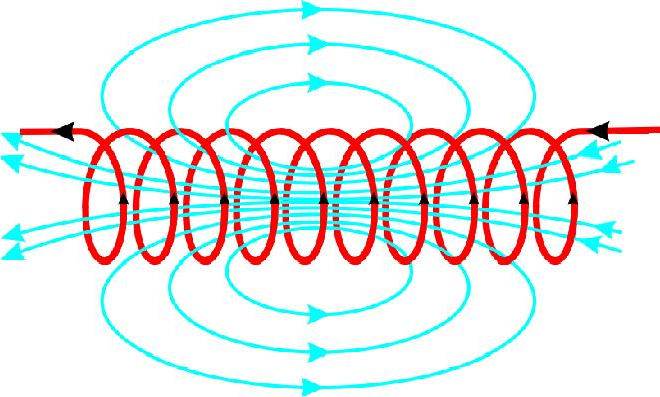
\includegraphics[height=2.5cm]{solenoid_field.png}};
  \node[anchor=south west,text width=8.2cm,font=\small,align=left] at ([xshift=1cm,yshift=0.35cm]current page.south west) {%
    \textbf{Complete classroom deck}: every derivation worked step by step with reasons, labelled diagrams, solved numericals, all textbook questions.\\[4pt]
    \textcolor{gray}{Figures: SCERT Class X Physical Science textbook, pp.\,219--248}};
\end{tikzpicture}
\end{frame}

% =====================================================================
\begin{frame}{Chapter roadmap}
\begin{columns}[T]
\column{0.5\textwidth}
\begin{tcolorbox}[colback=emblue!6,colframe=emblue,title={\textbf{Part A: Currents make magnetic fields}}]
\small
\begin{enumerate}
\item[10.1] Oersted experiment
\item[10.2] Magnetic field, field lines, flux $\Phi$, flux density $B$
\item[10.3] Field of a straight wire, circular coil, solenoid
\end{enumerate}
\end{tcolorbox}
\begin{tcolorbox}[colback=empurple!6,colframe=empurple,title={\textbf{Part B: Fields push on currents}}]
\small
\begin{enumerate}
\item[10.4] $F=qvB\sin\theta$, $F=ILB\sin\theta$, circular motion
\item[10.4] Electric motor
\end{enumerate}
\end{tcolorbox}
\column{0.5\textwidth}
\begin{tcolorbox}[colback=emgreen!6,colframe=emgreen,title={\textbf{Part C: Changing fields make currents}}]
\small
\begin{enumerate}
\item[10.5] Electromagnetic induction
\item[10.5] Faraday's law, Lenz's law
\item[10.5] Derivation: motional emf $\varepsilon=Blv$
\item[10.5] Applications, magnetic levitation
\item[10.5] AC and DC generators
\end{enumerate}
\end{tcolorbox}
\begin{examtip}[How to use this deck]
\small Badges \badge{1M} \badge{2M} \badge{4M} show usual marks. \textbf{Derivation} frames show \emph{step, working, reason}. Answers to \textbf{Teacher asks} appear on the next click.
\end{examtip}
\end{columns}
\end{frame}

% =====================================================================
\begin{frame}{Recall and warm-up}
\begin{columns}[c]
\column{0.52\textwidth}
\begin{itemize}
\item A magnet has two poles, N and S. Like poles repel, unlike poles attract.
\item A freely suspended magnet (compass needle) rests along the \textbf{north--south} direction.
\item A \textbf{field force} acts without contact (gravity, electric, magnetic).
\item Electric current = charges in motion: $I=\dfrac{Q}{t}$.
\item Electric power $P=\varepsilon I$; work $W=Fs$; power $P=Fv$.
\end{itemize}
\column{0.45\textwidth}
\begin{think}[Warm-up questions]
\small
\begin{itemize}
\item How do electric motors and calling bells work?
\item How does an electromagnet work?
\item Is there any relation between electricity and magnetism?
\item Can we produce electricity from magnetism?
\end{itemize}
\end{think}
\end{columns}
\end{frame}

% =====================================================================

\section{Basics first}

% =====================================================================
\begin{frame}{The big picture: one story in three steps}
\centering
\begin{tikzpicture}
\node[story=emblue] (a) at (-5.4,0) {\textbf{\faBolt\ Electric current}\\ moving charges};
\node[story=emteal] (b) at (0,0) {\textbf{\faMagnet\ Magnetic field}\\ appears around the current};
\node[story=emorange] (c) at (5.4,0) {\textbf{\faCog\ Motion}\\ the field pushes things};
\draw[-{Stealth},very thick,emblue] (a) -- node[above,font=\footnotesize,align=center]{\textbf{Part A}\\Oersted} (b);
\draw[-{Stealth},very thick,empurple] (b) -- node[above,font=\footnotesize,align=center]{\textbf{Part B}\\Motor} (c);
\draw[-{Stealth},very thick,emgreen,rounded corners=8pt] (c.south) -- ++(0,-1.3) -- node[below,font=\footnotesize]{\textbf{Part C}: moving a magnet makes current again (Generator)} ($(a.south)+(0,-1.3)$) -- (a.south);
\end{tikzpicture}
\vspace{6pt}
\begin{simple}[Remember this one line]
Electricity and magnetism are \textbf{two faces of the same thing}. Current makes magnetism; magnetism pushes current; changing magnetism makes current.
\end{simple}
\end{frame}
% =====================================================================
\begin{frame}{Basics 1: What is a magnet?}
\begin{columns}[c]
\column{0.5\textwidth}\centering
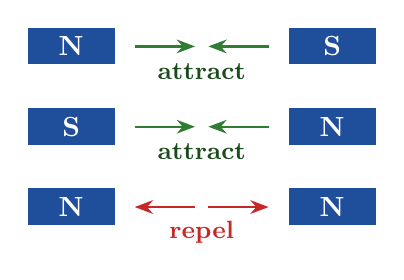
\begin{tikzpicture}[scale=0.85]
\foreach \y/\l/\r in {1.6/N/S,0.4/S/N,-0.8/N/N}{
 \ifx\l N \def\cl{emred}\else\def\cl{emblue}\fi
 \ifx\r N \def\cr{emred}\else\def\cr{emblue}\fi
 \fill[\cl] (-2.6,\y) rectangle (-1.3,\y+0.55); \node[white,font=\bfseries] at (-1.95,\y+0.27) {\l};
 \fill[\cr] (1.3,\y) rectangle (2.6,\y+0.55); \node[white,font=\bfseries] at (1.95,\y+0.27) {\r};}
\draw[-{Stealth},thick,emgreen] (-1.0,1.87) -- (-0.1,1.87); \draw[-{Stealth},thick,emgreen] (1.0,1.87) -- (0.1,1.87);
\node[font=\small\bfseries,emgreen!60!black] at (0,1.5) {attract};
\draw[-{Stealth},thick,emgreen] (-1.0,0.67) -- (-0.1,0.67); \draw[-{Stealth},thick,emgreen] (1.0,0.67) -- (0.1,0.67);
\node[font=\small\bfseries,emgreen!60!black] at (0,0.3) {attract};
\draw[-{Stealth},thick,emred] (-0.1,-0.53) -- (-1.0,-0.53); \draw[-{Stealth},thick,emred] (0.1,-0.53) -- (1.0,-0.53);
\node[font=\small\bfseries,emred] at (0,-0.9) {repel};
\end{tikzpicture}
\column{0.48\textwidth}
\begin{itemize}
\item Every magnet has \textbf{two poles}: North (N) and South (S).
\item \textbf{Unlike} poles attract. \textbf{Like} poles repel.
\item You can never get a single pole: cut a magnet and each piece has both N and S.
\item Magnets attract iron, nickel and cobalt.
\end{itemize}
\begin{simple}[Think of it like this]
A \textbf{compass needle} is a tiny magnet. Its N end always swings to the Earth's geographic north because the Earth itself acts like a giant magnet.
\end{simple}
\end{columns}
\end{frame}
% =====================================================================
\begin{frame}{Basics 2: What is a ``field''?}
\begin{columns}[c]
\column{0.5\textwidth}
\begin{simple}[Kitchen smell analogy]
Cooking in a kitchen: you smell it \textbf{without touching} the food.
\begin{itemize}
\item Strong smell near the stove; weak far away $\Rightarrow$ \textbf{strength} changes with place.
\item Smell drifts \emph{from} the stove \emph{towards} you $\Rightarrow$ it has a \textbf{direction}.
\end{itemize}
\end{simple}
\begin{defn}[Field]
\small Space around an object where it can push or pull other things \textbf{without touching}. A field has \key{strength} and \key{direction} at every point.
\end{defn}
\column{0.46\textwidth}\centering
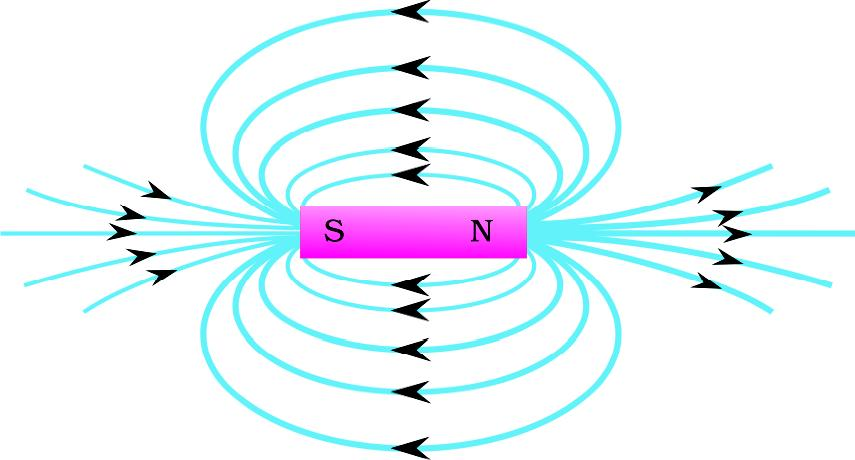
\includegraphics[width=0.95\linewidth]{bar_field.png}\\
{\scriptsize Magnetic field of a bar magnet. Each curve is a \textbf{field line}: the arrow shows the direction; crowded lines mean a stronger field.}
\end{columns}
\end{frame}
% =====================================================================
\begin{frame}{Basics 3: What is electric current?}
\begin{columns}[c]
\column{0.5\textwidth}\centering
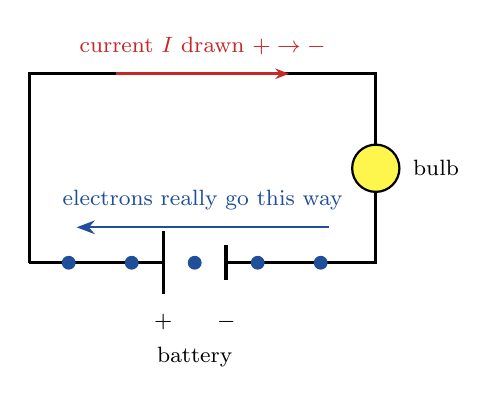
\begin{tikzpicture}
\draw[very thick] (0,0) -- (1.7,0) (2.5,0) -- (4.4,0) -- (4.4,0.9) (4.4,1.5) -- (4.4,2.4) -- (0,2.4) -- (0,0);
\draw[very thick] (1.7,-0.4) -- (1.7,0.4); \draw[ultra thick] (2.5,-0.22) -- (2.5,0.22);
\node[font=\footnotesize] at (1.7,-0.75) {$+$}; \node[font=\footnotesize] at (2.5,-0.75) {$-$};
\node[font=\footnotesize] at (2.1,-1.2) {battery};
\fill[yellow!70,draw=black,thick] (4.4,1.2) circle (0.3); \node[font=\footnotesize,anchor=west] at (4.75,1.2) {bulb};
\draw[cur] (1.1,2.4) -- (3.3,2.4) node[midway,above=3pt,font=\footnotesize,emred]{current $I$ drawn $+\to-$};
\foreach \x in {0.5,1.3,2.1,2.9,3.7}\fill[emblue] (\x,0) circle (2.5pt);
\draw[-{Stealth},emblue,thick] (3.8,0.45) -- (0.6,0.45);
\node[font=\footnotesize,emblue] at (2.2,0.8) {electrons really go this way};
\end{tikzpicture}
\column{0.48\textwidth}
\begin{itemize}
\item Current is the \textbf{flow of charge}, like water flowing in a pipe.
\item Battery = pump, wire = pipe, charge = water.
\end{itemize}
\begin{formula}[Current]
\[I=\frac{Q}{t}\quad\text{unit: ampere (A)}\]
\small $1\,\text{A}=1$ coulomb of charge per second.
\end{formula}
\begin{simple}[Direction convention]
We \textbf{draw} current from $+$ to $-$ (old convention). Electrons really go the other way. Always follow the \textbf{drawn} direction in this chapter.
\end{simple}
\end{columns}
\end{frame}
% =====================================================================
\begin{frame}{Basics 4: Reading arrows into and out of the page}
\begin{columns}[c]
\column{0.5\textwidth}\centering
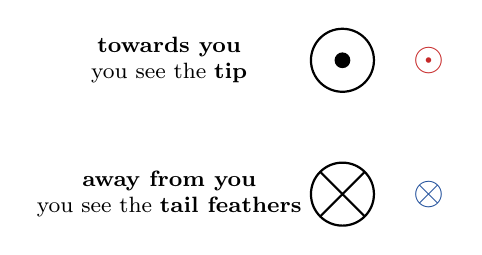
\begin{tikzpicture}
% dart side view
% toward you
\node[font=\footnotesize,align=center] at (0.2,0.2) {\textbf{towards you}\\you see the \textbf{tip}};
\draw[thick,fill=white] (2.4,0.2) circle (0.4); \fill (2.4,0.2) circle (0.1);
\node[font=\Large\bfseries,emred] at (3.5,0.2) {$\odot$};
% away
\node[font=\footnotesize,align=center] at (0.2,-1.5) {\textbf{away from you}\\you see the \textbf{tail feathers}};
\draw[thick,fill=white] (2.4,-1.5) circle (0.4); \draw[thick] (2.4-0.28,-1.5-0.28)--(2.4+0.28,-1.5+0.28) (2.4-0.28,-1.5+0.28)--(2.4+0.28,-1.5-0.28);
\node[font=\Large\bfseries,emblue] at (3.5,-1.5) {$\otimes$};
\end{tikzpicture}
\column{0.48\textwidth}
\begin{itemize}
\item $\odot$ (dot) $\Rightarrow$ pointing \textbf{out of the page}, towards you.
\item $\otimes$ (cross) $\Rightarrow$ pointing \textbf{into the page}, away from you.
\item A page full of $\times$ means a magnetic field going \textbf{into} the page; full of $\cdot$ means \textbf{out}.
\end{itemize}
\begin{simple}[Memory trick]
\textbf{D}ot = \textbf{D}ooming at you (the \emph{tip} is coming at you).\\ \textbf{C}ross = \textbf{C}arrying away (you see the \emph{tail}, it is leaving).
\end{simple}
\end{columns}
\end{frame}
% =====================================================================
\begin{frame}{Basics 5: Your right hand is the tool of this chapter}
\begin{columns}[T]
\column{0.33\textwidth}\centering
\textbf{\color{emblue}Rule 1: thumb rule}\\[2pt]
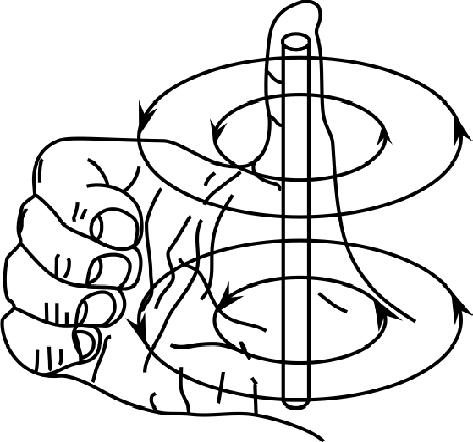
\includegraphics[height=2.4cm]{thumb_rule.png}\\
{\small Straight wire.\\ \textbf{Thumb} = current.\\ \textbf{Curled fingers} = field.}
\column{0.33\textwidth}\centering
\textbf{\color{emteal}Rule 2: coil rule}\\[2pt]
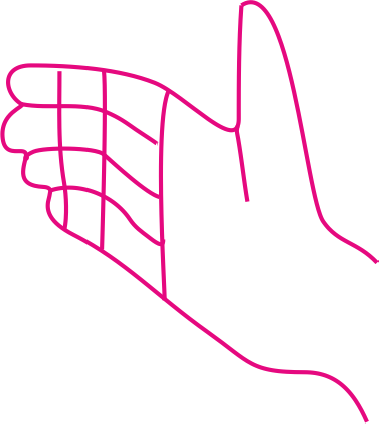
\includegraphics[height=2.4cm]{coil_hand.png}\\
{\small Coil or solenoid.\\ \textbf{Curled fingers} = current.\\ \textbf{Thumb} = N pole.}
\column{0.33\textwidth}\centering
\textbf{\color{emorange}Rule 3: force rule}\\[2pt]

\includegraphics[height=2.4cm]{rh_rule_b.png}\\
{\small Force on current/charge.\\ \textbf{Forefinger} = current $I$ (or $v$),\\ \textbf{middle finger} = field $B$,\\ \textbf{thumb} = force $F$.}
\end{columns}
\vspace{4pt}
\begin{simple}[Always ask: ``What do I know, and what do I want?'']
Know the \textbf{current}, want the \textbf{field}? Rule 1 or 2. Know the \textbf{current and field}, want the \textbf{push}? Rule 3. Use your \textbf{right} hand only.
\end{simple}
\end{frame}
% =====================================================================
\begin{frame}{Basics 6: Symbols and units you will meet}
\centering\renewcommand{\arraystretch}{1.25}
\begin{tabular}{@{}llll@{}}
\toprule
\textbf{Quantity} & \textbf{Symbol} & \textbf{SI unit} & \textbf{In plain words}\\
\midrule
Electric current & $I$ & ampere (A) & how fast charge flows\\
Charge & $q$ or $Q$ & coulomb (C) & amount of electric charge\\
Velocity & $v$ & m/s & speed with direction\\
Magnetic flux density & $B$ & tesla (T) & strength of the field\\
Magnetic flux & $\Phi$ & weber (Wb) & total field passing through an area\\
Force & $F$ & newton (N) & a push or pull\\
Induced emf & $\varepsilon$ & volt (V) & electrical ``push'' that drives current\\
\bottomrule
\end{tabular}
\vspace{4pt}
\begin{examtip}[Unit tip]
$1\,\text{T}=1\,\text{Wb/m}^2$. Convert first: cm $\to$ m, cm$^2\to$ m$^2$ (divide by $10^4$), before substituting into formulas.
\end{examtip}
\end{frame}
% =====================================================================
\begin{frame}{Maths 1: Powers of ten (scientific notation)}
\begin{columns}[T]
\column{0.5\textwidth}
\begin{simple}[Why?]
Physics numbers can be huge or tiny. Charge of a proton: $0.00000000000000000016$ C. Write it as $\mathbf{1.6\times10^{-19}}$ C.
\end{simple}
\begin{itemize}
\item $10^{3}=1000$,\; $10^{-3}=\dfrac{1}{1000}=0.001$
\item Move the point \textbf{left} $\Rightarrow$ power goes \textbf{up}; move \textbf{right} $\Rightarrow$ power goes \textbf{down}.
\end{itemize}
\column{0.48\textwidth}
\begin{formula}[Rules]
\[10^{a}\times10^{b}=10^{a+b}\qquad\frac{10^{a}}{10^{b}}=10^{a-b}\]
\end{formula}
\begin{answer}[Worked example]
$(2\times10^{6})\times(1.6\times10^{-19})\times0.5$\\
Numbers: $2\times1.6\times0.5=1.6$\\
Powers: $10^{6-19}=10^{-13}$\\
Answer: $\mathbf{1.6\times10^{-13}}$
\end{answer}
\end{columns}
\end{frame}
% =====================================================================
\begin{frame}{Maths 2: Changing units before you calculate}
\centering\renewcommand{\arraystretch}{1.25}
\begin{tabular}{@{}lll@{}}
\toprule
\textbf{Change} & \textbf{How} & \textbf{Example}\\
\midrule
cm $\to$ m & divide by 100 & $20\ \text{cm}=0.2$ m\\
mm $\to$ m & divide by 1000 & $5.7$ mm $=5.7\times10^{-3}$ m\\
cm$^2\to$ m$^2$ & divide by $10^{4}$ (not 100!) & $4\ \text{cm}^2=4\times10^{-4}$ m$^2$\\
minutes $\to$ s & multiply by 60 & $0.2$ min $=12$ s\\
\bottomrule
\end{tabular}
\vspace{6pt}
\begin{simple}[Why $10^4$ for area?]
$1\ \text{cm}=\frac{1}{100}$ m, so $1\ \text{cm}^2=\frac{1}{100}\times\frac{1}{100}=\frac{1}{10\,000}$ m$^2$. Area squares the conversion factor.
\end{simple}
\end{frame}
% =====================================================================
\begin{frame}{Maths 3: Rearranging a formula (the balance method)}
\begin{columns}[T]
\column{0.5\textwidth}
\begin{simple}[Golden rule]
An equation is a balance. Whatever you do to one side, do the \textbf{same} to the other.
\end{simple}
Start with $F=ILB$.
\begin{itemize}
\item Find $B$: divide both sides by $IL$ $\Rightarrow$ $B=\dfrac{F}{IL}$
\item Find $I$: divide both sides by $LB$ $\Rightarrow$ $I=\dfrac{F}{LB}$
\item Find $L$: divide both sides by $IB$ $\Rightarrow$ $L=\dfrac{F}{IB}$
\end{itemize}
\column{0.48\textwidth}
\begin{answer}[Example from the chapter]
$r=\dfrac{mv}{Bq}$. Find $v$.\\[3pt]
Multiply both sides by $Bq$: $rBq=mv$\\
Divide both sides by $m$: $v=\dfrac{rBq}{m}$
\end{answer}
\begin{examtip}[Steps for every numerical]
1. Write the formula. 2. Convert units. 3. Rearrange if needed. 4. Substitute. 5. Calculate and write the \textbf{unit}.
\end{examtip}
\end{columns}
\end{frame}
% =====================================================================
\begin{frame}{Maths 4: Sine and cosine of an angle}
\begin{columns}[c]
\column{0.42\textwidth}\centering
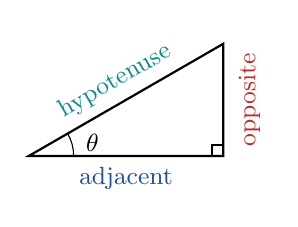
\begin{tikzpicture}[scale=0.95]
\draw[thick] (0,0) -- (2.6,0) -- (2.6,1.5) -- cycle;
\draw[thick] (2.45,0) -- (2.45,0.15) -- (2.6,0.15);
\draw (0.6,0) arc (0:30:0.6); \node[font=\small] at (0.85,0.17) {$\theta$};
\node[font=\small,emblue] at (1.3,-0.3) {adjacent};
\node[font=\small,emred,rotate=90] at (2.95,0.75) {opposite};
\node[font=\small,emteal,rotate=30] at (1.15,1.0) {hypotenuse};
\end{tikzpicture}
{\small$\sin\theta=\dfrac{\text{opposite}}{\text{hypotenuse}}$\\[4pt]$\cos\theta=\dfrac{\text{adjacent}}{\text{hypotenuse}}$}
\column{0.56\textwidth}
\small\centering\renewcommand{\arraystretch}{1.2}
\begin{tabular}{@{}c|ccccc@{}}
$\theta$ & $0^\circ$ & $30^\circ$ & $45^\circ$ & $60^\circ$ & $90^\circ$\\\hline
$\sin\theta$ & $0$ & $\tfrac12$ & $\tfrac{1}{\sqrt2}$ & $\tfrac{\sqrt3}{2}$ & $1$\\
$\cos\theta$ & $1$ & $\tfrac{\sqrt3}{2}$ & $\tfrac{1}{\sqrt2}$ & $\tfrac12$ & $0$\\
\end{tabular}
\vspace{4pt}
\begin{simple}[Where we use them]
$F=qvB\sin\theta$: $\theta$ is the angle between $v$ and $B$. At $90^\circ$ the force is maximum; at $0^\circ$ it is zero.\\
$\Phi=BA\cos\theta$: $\theta$ is the angle between $B$ and the \textbf{normal} to the plane. At $0^\circ$ the flux is maximum.
\end{simple}
\end{columns}
\end{frame}
% =====================================================================
\begin{frame}{Maths 5: Area, circles and time period}
\begin{columns}[T]
\column{0.5\textwidth}
\begin{formula}[Shapes]
\small Rectangle: $A=\text{length}\times\text{breadth}$\\
Circle: $A=\pi r^{2}$, circumference $=2\pi r$ ($\pi\approx3.14$)
\end{formula}
\begin{answer}[Example]
Loop of radius $0.1$ m: $A=3.14\times0.1^{2}=0.0314$ m$^{2}$.
\end{answer}
\column{0.48\textwidth}
\begin{formula}[Speed, distance, time]
\[v=\frac{\text{distance}}{\text{time}}\;\Rightarrow\;\text{time}=\frac{\text{distance}}{v}\]
\end{formula}
\begin{simple}[Time period $T$]
Time for one full circle: $T=\dfrac{2\pi r}{v}$. We use this in the circular-path derivation.
\end{simple}
\end{columns}
\end{frame}
% =====================================================================
\begin{frame}{Maths 6: ``Change'' and ``rate of change'' ($\Delta$)}
\begin{columns}[c]
\column{0.5\textwidth}
\begin{itemize}
\item $\Delta$ (delta) means \textbf{change} = final $-$ initial.
\item $\Delta\Phi=\Phi_{\text{final}}-\Phi_{\text{initial}}$,\quad $\Delta t=t_{\text{final}}-t_{\text{initial}}$
\item \textbf{Rate of change} = change $\div$ time taken, e.g.\ $\varepsilon=\dfrac{\Delta\Phi}{\Delta t}$.
\end{itemize}
\begin{answer}[Example]
Flux falls from $0.5$ Wb to $0.1$ Wb in $0.2$ s.\\
$\Delta\Phi=0.1-0.5=-0.4$ Wb\\
$|\varepsilon|=\dfrac{0.4}{0.2}=\mathbf{2}$ V
\end{answer}
\column{0.46\textwidth}\centering
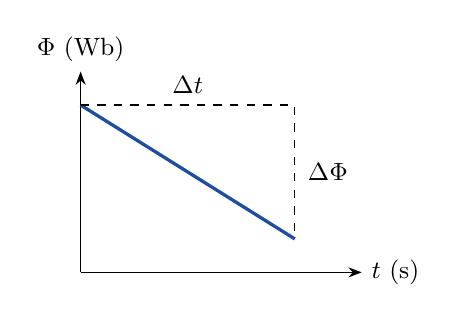
\begin{tikzpicture}[scale=0.85]
\draw[-{Stealth}] (0,0) -- (4.2,0) node[right,font=\small]{$t$ (s)};
\draw[-{Stealth}] (0,0) -- (0,3) node[above,font=\small]{$\Phi$ (Wb)};
\draw[very thick,emblue] (0,2.5) -- (3.2,0.5);
\draw[dashed] (0,2.5) -- (3.2,2.5) -- (3.2,0.5);
\node[font=\small] at (1.6,2.8) {$\Delta t$}; \node[font=\small,anchor=west] at (3.25,1.5) {$\Delta\Phi$};
\end{tikzpicture}\\
{\small Slope of a flux--time graph = $\dfrac{\Delta\Phi}{\Delta t}$ = induced emf. A steeper line means a bigger emf; a flat line means zero emf.}
\end{columns}
\end{frame}
% =====================================================================
\begin{frame}{Maths 7: Proportion, ``if this doubles, what happens?''}
\begin{columns}[T]
\column{0.55\textwidth}
\renewcommand{\arraystretch}{1.3}\small
\begin{tabular}{@{}lll@{}}
\toprule
\textbf{Formula} & \textbf{If this doubles\ldots} & \textbf{That}\\
\midrule
$F=ILB$ & $B$ doubles & $F$ doubles\\
$F=ILB$ & $I$ and $L$ both double & $F$ becomes $4\times$\\
$r=\dfrac{mv}{Bq}$ & $B$ doubles & $r$ \textbf{halves}\\
$\varepsilon=Blv$ & $v$ doubles & $\varepsilon$ doubles\\
$\Phi=BA\cos\theta$ & $A$ doubles & $\Phi$ doubles\\
\bottomrule
\end{tabular}
\column{0.43\textwidth}
\begin{simple}[Two kinds of relation]
\textbf{Direct} ($F\propto B$): both grow together.\\
\textbf{Inverse} ($r\propto\frac{1}{B}$): one grows, the other shrinks.
\end{simple}
\begin{examtip}
Spot the variable on top (direct) or underneath (inverse) in the formula.
\end{examtip}
\end{columns}
\end{frame}
% =====================================================================
\begin{frame}{Maths check: try these}
\small
\begin{columns}[T]
\column{0.5\textwidth}
\begin{think}[Quick maths drill]
\begin{enumerate}
\item Write $0.0005$ in powers of ten.
\item Convert $50$ cm$^2$ to m$^2$.
\item $F=ILB$: find $L$ if $F=6$ N, $I=3$ A, $B=0.5$ T.
\item Value of $\sin30^\circ$ and $\cos60^\circ$?
\item Flux changes by $0.6$ Wb in $0.3$ s. Find $\varepsilon$.
\end{enumerate}
\end{think}
\column{0.46\textwidth}
\uncover<2->{\begin{answer}[Answers]
\begin{enumerate}
\item $5\times10^{-4}$
\item $5\times10^{-3}$ m$^2$
\item $L=\dfrac{6}{3\times0.5}=4$ m
\item both $\tfrac12$
\item $\varepsilon=\dfrac{0.6}{0.3}=2$ V
\end{enumerate}
\end{answer}}
\end{columns}
\end{frame}
% =====================================================================
\begin{frame}{Quick check before we start}
\small
\begin{columns}[T]
\column{0.5\textwidth}
\begin{think}[Try these (answers on the next click)]
\begin{enumerate}
\item Two N poles are brought close. Attract or repel?
\item Charge $6$ C flows in $2$ s. Find the current.
\item An arrow shows $\otimes$. Is it going into or out of the page?
\item Which hand do we use for the rules?
\end{enumerate}
\end{think}
\column{0.46\textwidth}
\uncover<2->{\begin{answer}[Answers]
\begin{enumerate}
\item Repel (like poles).
\item $I=Q/t=6/2=3$ A.
\item Into the page.
\item The right hand.
\end{enumerate}
\end{answer}}
\end{columns}
\end{frame}

\section{Part A: Magnetic field}
% =====================================================================
\begin{frame}{Part A: Currents make magnetic fields}
\begin{goals}
\large\begin{itemize}
\item Describe what Oersted observed and what it proves.
\item Draw and read \textbf{magnetic field lines}; tell a strong field from a weak one.
\item Explain \textbf{flux} $\Phi$ and \textbf{flux density} $B$, and use $\Phi=BA\cos\theta$.
\item Find the field direction around a wire, a coil and a solenoid with the \textbf{right hand rule}.
\end{itemize}
\end{goals}
\end{frame}

\begin{frame}{10.1 Oersted experiment (Activity 1) \hfill \badge{2M} \badge{4M}}
\begin{columns}[T]
\column{0.56\textwidth}
\centering
\figlab{oersted_setup.png}{width=\linewidth}{
\draw[fptr] (0.30,1.12) node[flab,anchor=south east]{copper wire (24 gauge)} -- (0.36,0.82);
\draw[fptr] (0.36,1.12) node[flab,anchor=south west]{wooden sticks} -- (0.50,0.95);
\draw[fptr] (0.36,1.12) -- (0.27,0.62);
\draw[fptr] (0.30,0.20) node[flab,anchor=north]{magnetic compass} -- (0.40,0.60);
\draw[fptr] (0.85,1.10) node[flab,anchor=south]{battery (3 V)} -- (0.66,0.78);
\draw[fptr] (0.72,0.10) node[flab,anchor=north]{key} -- (0.54,0.40);
\draw[fptr] (0.05,0.05) node[flab,anchor=north]{thermocol sheet} -- (0.15,0.40);}\\[12pt]
{\scriptsize fig-1: current-carrying wire above a compass}
\column{0.42\textwidth}
\small
\begin{enumerate}
\item Wire stretched through slits of two sticks, in series with battery and key. Compass below the wire.
\item Bring a bar magnet near: needle deflects (magnetic force).
\item Remove the magnet, switch \textbf{on}: needle \textbf{deflects again}!
\item Switch off: needle returns to N--S.
\end{enumerate}
\begin{answer}[Conclusion]
\small A \textbf{current-carrying wire produces a magnetic field} around it. Electricity and magnetism are related.
\end{answer}
\end{columns}
\end{frame}

% =====================================================================
\begin{frame}{Do you know? Hans Christian Oersted \hfill \badge{1M}}
\begin{columns}[c]
\column{0.26\textwidth}\centering
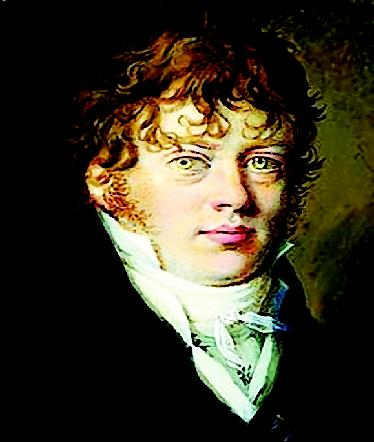
\includegraphics[width=0.9\linewidth]{oersted.png}\\{\scriptsize H.\,C.\ Oersted (1777--1851)}
\column{0.72\textwidth}
\begin{itemize}
\item In a lecture in April 1820 he placed a compass needle under a wire and switched on the current: the needle \textbf{deflected}.
\item Showed that electricity and magnetism are \textbf{interconnected}: the start of \key{electromagnetism}.
\item Led to the dynamo, the electric motor, radio, television and fibre optics.
\item The unit of magnetic field strength is named \imp{oersted} in his honour.
\end{itemize}
\end{columns}
\end{frame}

% =====================================================================
\begin{frame}{10.2 Magnetic field of a bar magnet (Activity 2) \hfill \badge{1M} \badge{2M}}
\begin{columns}[T]
\column{0.55\textwidth}
\begin{activity}[Activity 2: compass around a bar magnet]
\small Place a compass at many points around a bar magnet on paper. Mark the direction of the needle at each point (S $\to$ N of the needle).
\end{activity}
\small
\begin{itemize}
\item The needle points in \textbf{different directions} at different places $\Rightarrow$ the field has \textbf{direction} that varies from point to point.
\item Far from the magnet the needle points almost N--S $\Rightarrow$ \textbf{strength} decreases with distance.
\item Above the magnet the needle is also deflected $\Rightarrow$ the field is \textbf{three-dimensional}.
\end{itemize}
\column{0.43\textwidth}
\begin{defn}[Field]
\small A region where a force acts on an object \textbf{without physical contact}.
\end{defn}
\begin{defn}[Magnetic field]
\small The region surrounding a magnet in which its magnetic force can be felt. It is characterised by \key{strength} and \key{direction}.
\end{defn}
\end{columns}
\end{frame}

% =====================================================================
\begin{frame}{10.2.1 Magnetic field lines (Activity 3) \hfill \badge{1M} \badge{2M} \badge{Diagram}}
\begin{columns}[c]
\column{0.5\textwidth}\centering
\figlab{bar_field.png}{width=\linewidth}{
\draw[fptr] (0.12,1.08) node[flab,anchor=south]{field line} -- (0.30,0.93);
\draw[fptr] (0.88,1.08) node[flab,anchor=south]{lines crowded near poles (strong)} -- (0.72,0.62);
\draw[fptr] (0.50,-0.10) node[flab,anchor=north]{lines far apart (weak)} -- (0.50,0.04);}\\[12pt]
{\scriptsize fig-2: field lines of a bar magnet (outside: N $\to$ S)}
\column{0.48\textwidth}
\small
\textbf{Plotting:} put the compass at N, mark a dot at the tip of the needle, move the compass to the dot, repeat until you reach S. Join the dots.
\begin{itemize}
\item Field lines are \textbf{imaginary} curves.
\item \key{Tangent} at any point gives the direction of the field.
\item \textbf{Crowded} lines $\Rightarrow$ strong field; \textbf{spread} lines $\Rightarrow$ weak field.
\item \key{Non-uniform field}: strength \textbf{or} direction changes.\\ \key{Uniform field}: strength \textbf{and} direction constant (parallel, equally spaced lines).
\end{itemize}
\end{columns}
\end{frame}

% =====================================================================
\begin{frame}{10.2.2 Magnetic flux and flux density \hfill \badge{1M} \badge{2M}}
\begin{columns}[c]
\column{0.44\textwidth}\centering
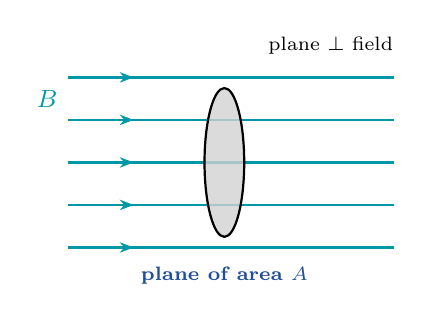
\begin{tikzpicture}[scale=0.9]
\foreach \y in {-1.2,-0.6,0,0.6,1.2} \draw[fl=0.2] (-2.2,\y) -- (2.4,\y);
\fill[gray!35,opacity=0.8] (0,0) ellipse (0.28 and 1.05);
\draw[thick] (0,0) ellipse (0.28 and 1.05);
\node[flab] at (0.0,-1.6) {plane of area $A$};
\node[font=\small\bfseries,fieldc] at (-2.5,0.9) {$B$};
\node[font=\scriptsize,align=center] at (1.5,1.65) {plane $\perp$ field};
\end{tikzpicture}\\
{\scriptsize fig-3(a): lines crossing a plane placed perpendicular to a uniform field}
\column{0.54\textwidth}
\begin{defn}[Magnetic flux $\Phi$]
\small The number of field lines passing through a plane of area $A$ held \textbf{perpendicular} to the field. SI unit: \key{weber (Wb)}.
\end{defn}
\begin{defn}[Magnetic flux density $B$]
\small Flux passing through \textbf{unit area} held perpendicular to the field. Also called \key{magnetic induction}.
\[B=\frac{\Phi}{A}\qquad\text{unit: Wb/m}^2=\text{tesla (T)}\]
\end{defn}
\end{columns}
\end{frame}

% =====================================================================
\begin{frame}[shrink=8]{Flux in simple words: rain through a window}
\begin{columns}[c]
\column{0.6\textwidth}\centering
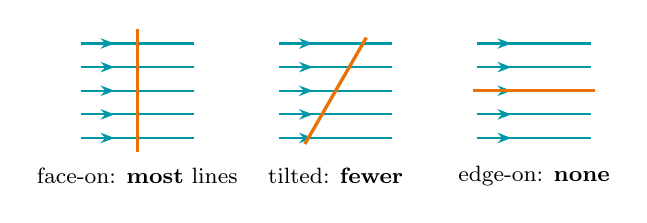
\begin{tikzpicture}[scale=0.6]
\foreach \ang/\xo/\lab in {90/0/{face-on: \textbf{most} lines},60/4.2/{tilted: \textbf{fewer}},0/8.4/{edge-on: \textbf{none}}}{
 \foreach \y in {-1.0,-0.5,0,0.5,1.0} \draw[fl=0.3] (\xo-1.2,\y) -- (\xo+1.2,\y);
 \draw[very thick,emorange] ($(\xo,0)+(\ang:1.3)$) -- ($(\xo,0)-(\ang:1.3)$);
 \node[font=\footnotesize,align=center] at (\xo,-1.8) {\lab};}
\end{tikzpicture}\\
{\scriptsize Orange line = the window seen edge-on; blue lines = field lines (rain).}
\column{0.38\textwidth}
\begin{simple}[Analogy]
Rain = field lines. Window = area $A$.
\begin{itemize}
\item Hold the window \textbf{face-on}: the most rain passes.
\item \textbf{Tilt} it: less passes.
\item \textbf{Edge-on}: no rain passes.
\end{itemize}
\textbf{Flux $\Phi$} = how much rain passes. \textbf{Flux density $B$} = how heavy the rain is.
\end{simple}
\end{columns}
\end{frame}

% =====================================================================
\begin{frame}[shrink=15]{Derivation 1: flux through a tilted plane, $\Phi=BA\cos\theta$ \hfill \badge{2M}}
\begin{columns}[T]
\column{0.4\textwidth}\centering
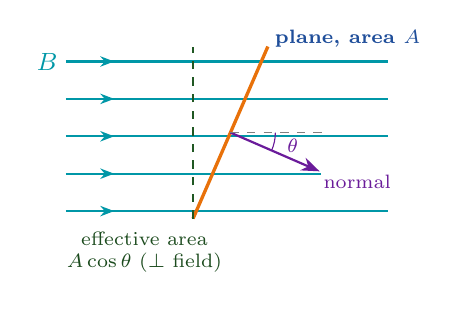
\begin{tikzpicture}[scale=0.95]
\foreach \y in {0.2,0.7,1.2,1.7,2.2} \draw[fl=0.15] (-0.5,\y) -- (3.8,\y);
\node[font=\small\bfseries,fieldc] at (-0.75,2.2) {$B$};
% tilted plane (edge view)
\draw[very thick,emorange] (1.2,0.1) -- (2.2,2.4);
\node[flab,anchor=west] at (2.25,2.5) {plane, area $A$};
% normal
\coordinate (C) at (1.7,1.25);
\draw[-{Stealth},thick,empurple] (C) -- ($(C)+(-23.5:1.3)$) node[below right,font=\scriptsize,empurple,fill=white,inner sep=1pt]{normal};
\draw[dashed,gray] (C) -- ($(C)+(1.3,0)$);
\draw[empurple] ($(C)+(0.6,0)$) arc (0:-23.5:0.6); \node[font=\scriptsize,empurple] at ($(C)+(-12:0.85)$) {$\theta$};
% projection perpendicular to field
\draw[thick,dashed,emgreen!70!black] (1.2,0.1) -- (1.2,2.4);
\node[font=\scriptsize,emgreen!60!black,align=center] at (0.55,-0.35) {effective area\\$A\cos\theta$ ($\perp$ field)};
\end{tikzpicture}\\
{\scriptsize fig-3(b): edge view of the plane}
\column{0.58\textwidth}
\begin{steps}[3.3cm]
\stp1 & B=\frac{\Phi}{A_{\perp}} & $B$ is always defined with the area \textbf{perpendicular} to the field\\
\stp2 & A_{\perp}=A\cos\theta & $\theta$ = angle between $B$ and the normal; only this part of the plane faces the field\\
\stp3 & B=\frac{\Phi}{A\cos\theta} & substitute step 2 in step 1\\
\stp4 & \Phi=BA\cos\theta & multiply both sides by $A\cos\theta$\\
\end{steps}
\begin{formula}[Special cases]
\small $\theta=0^\circ$ (plane $\perp$ field): $\Phi=BA$ (maximum)\\
$\theta=90^\circ$ (plane $\parallel$ field): $\Phi=BA\cos90^\circ=0$
\end{formula}
\end{columns}
\end{frame}

% =====================================================================
\begin{frame}{Solved numericals: flux and flux density \hfill \badge{2M}}
\small
\begin{columns}[T]
\column{0.5\textwidth}
\begin{tcolorbox}[colback=emblue!4,colframe=emblue,title={\textbf{Q1.} $B=0.5$ T through a loop of area $0.02$ m$^2$, loop $\perp$ field. Find $\Phi$.}]
\stp1 Plane $\perp$ field $\Rightarrow\theta=0^\circ$, $\cos0^\circ=1$.\\
\stp2 $\Phi=BA=0.5\times0.02=\boxed{0.01\ \text{Wb}}$
\end{tcolorbox}
\pause
\begin{tcolorbox}[colback=emblue!4,colframe=emblue,title={\textbf{Q2.} Same loop turned so the normal makes $60^\circ$ with $B$.}]
\stp1 $\Phi=BA\cos60^\circ=0.01\times\frac12=\boxed{0.005\ \text{Wb}}$
\end{tcolorbox}
\column{0.5\textwidth}
\pause
\begin{tcolorbox}[colback=emgreen!5,colframe=emgreen,title={\textbf{Q3.} Flux of $2\times10^{-3}$ Wb crosses $4$ cm$^2$ normally. Find $B$.}]
\stp1 $A=4\ \text{cm}^2=4\times10^{-4}$ m$^2$ \;(1 cm$^2=10^{-4}$ m$^2$)\\[2pt]
\stp2 $B=\dfrac{\Phi}{A}=\dfrac{2\times10^{-3}}{4\times10^{-4}}=\boxed{5\ \text{T}}$
\end{tcolorbox}
\pause
\begin{think}[Textbook question]
\small What is the flux through a plane held \textbf{parallel} to the field?\\
\onslide<5->{\textbf{Zero}: no field line crosses it ($\theta=90^\circ$).}
\end{think}
\end{columns}
\end{frame}

% =====================================================================
\begin{frame}{10.3.1 Field of a straight current-carrying wire (Activity 4) \hfill \badge{2M} \badge{4M}}
\begin{columns}[T]
\column{0.42\textwidth}\centering
\figlab{wire_setup.png}{height=0.6\textheight}{
\draw[fptr] (0.30,0.97) node[flab,anchor=south]{retort stand} -- (0.58,0.92);
\draw[fptr] (1.05,0.97) node[flab,anchor=south]{vertical wire} -- (0.84,0.75);
\draw[fptr] (1.02,0.02) node[flab,anchor=north]{compass needles} -- (0.85,0.51);
\draw[fptr] (0.62,0.02) node[flab,anchor=north]{plank} -- (0.70,0.50);
\draw[fptr] (-0.05,0.70) node[flab,anchor=east]{battery} -- (0.27,0.52);
\draw[fptr] (-0.05,0.45) node[flab,anchor=east]{switch} -- (0.38,0.49);
\draw[fptr] (-0.05,0.25) node[flab,anchor=east]{table} -- (0.10,0.35);}\\
{\scriptsize fig-4(a)}
\column{0.56\textwidth}
\small
\begin{enumerate}
\item Pass a vertical wire through a hole in a plank; place 6--10 compass needles on a circle around the hole.
\item Switch on (3 V battery).
\item The needles set along \textbf{tangents to the circle}.
\item Sprinkle iron filings: they form \textbf{concentric circles}.
\end{enumerate}
\begin{answer}[Conclusion]
\small Field lines of a straight wire are \textbf{concentric circles} centred on the wire, in a plane perpendicular to it. They are \imp{closed loops}. The field is stronger near the wire (circles closer).
\end{answer}
\end{columns}
\end{frame}

% =====================================================================
\begin{frame}[shrink=6]{Direction of the field: right hand thumb rule \hfill \badge{1M} \badge{2M}}
\begin{columns}[c]
\column{0.28\textwidth}\centering
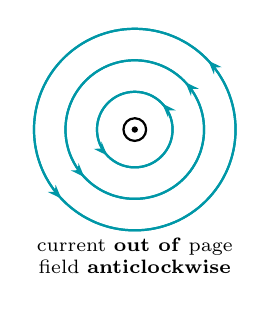
\begin{tikzpicture}[scale=0.8]
\foreach \r/\p in {0.6/0.12,1.1/0.12,1.6/0.12} \draw[fl=\p] (0,0) circle (\r);
\foreach \r/\p in {0.6/0.62,1.1/0.62,1.6/0.62} \draw[fieldc,thick,postaction={decorate},decoration={markings,mark=at position \p with {\arrow{Stealth[length=5pt]}}}] (0,0) circle (\r);
\outpage{(0,0)}
\node[font=\scriptsize,align=center] at (0,-2.0) {current \textbf{out of} page\\field \textbf{anticlockwise}};
\end{tikzpicture}\\{\scriptsize fig-4(b)}
\column{0.28\textwidth}\centering
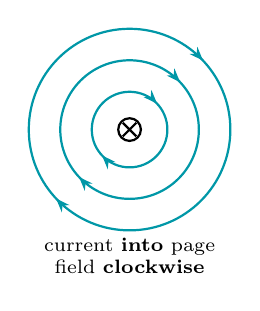
\begin{tikzpicture}[scale=0.8]
\foreach \r in {0.6,1.1,1.6} \draw[fieldc,thick,postaction={decorate},decoration={markings,mark=at position 0.12 with {\arrowreversed{Stealth[length=5pt]}},mark=at position 0.62 with {\arrowreversed{Stealth[length=5pt]}}}] (0,0) circle (\r);
\inpage{(0,0)}
\node[font=\scriptsize,align=center] at (0,-2.0) {current \textbf{into} page\\field \textbf{clockwise}};
\end{tikzpicture}\\{\scriptsize fig-4(c)}
\column{0.42\textwidth}\centering
\figlab{thumb_rule.png}{width=0.62\linewidth}{
\draw[cur] (0.63,0.80) -- (0.63,1.08) node[above,font=\scriptsize\bfseries,emred]{thumb: current $I$};
\draw[fptr] (1.10,0.55) node[flab,anchor=west,align=left]{fingers:\\field $B$} -- (0.97,0.72);}\\
{\scriptsize fig-4(d)}
\begin{defn}[Right hand thumb rule]
\small Grasp the wire with the right hand with the \textbf{thumb along the current}; the \textbf{curled fingers} give the direction of the field lines.
\end{defn}
\end{columns}
\vspace{2pt}
{\scriptsize Symbols: $\odot$ current/field out of the page (arrow tip);\quad $\otimes$ into the page (arrow tail).}
\end{frame}

% =====================================================================
\begin{frame}{10.3.2 Field of a circular coil (Activity 5) \hfill \badge{2M} \badge{4M}}
\begin{columns}[T]
\column{0.42\textwidth}\centering
\figlab{coil_setup.png}{width=0.95\linewidth}{
\draw[fptr] (0.10,1.08) node[flab,anchor=south]{circular coil (4--5 turns)} -- (0.34,0.90);
\draw[fptr] (0.62,1.08) node[flab,anchor=south]{compass at centre} -- (0.50,0.70);
\draw[fptr] (0.72,-0.06) node[flab,anchor=north]{to current supply} -- (0.88,0.58);
\draw[fptr] (0.72,-0.06) -- (0.64,0.30);}\\[8pt]
{\scriptsize fig-5(a)}
\column{0.56\textwidth}
\small
\begin{itemize}
\item Plot field lines with a compass around the coil.
\item At the centre the needle points \textbf{perpendicular to the plane of the coil}: the field there is along the axis.
\item Bring a compass near one face: its S pole points to the face $\Rightarrow$ that face acts as a \textbf{N pole}.
\end{itemize}
\begin{defn}[Right hand rule for a coil]
\small Curl the right-hand fingers along the \textbf{current}; the \textbf{thumb} gives the direction of the \textbf{field} (points out of the N face).
\end{defn}
\end{columns}
\end{frame}

\begin{frame}{Coil: which face is North? \hfill \badge{1M} \badge{2M}}
\begin{columns}[c]
\column{0.3\textwidth}\centering
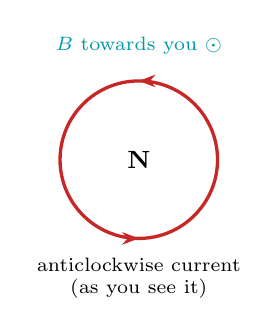
\begin{tikzpicture}
\draw[emred,very thick,postaction={decorate},decoration={markings,mark=at position 0.25 with {\arrow{Stealth[length=6pt]}},mark=at position 0.75 with {\arrow{Stealth[length=6pt]}}}] (0,0) circle (1);
\node[font=\small\bfseries] at (0,0) {N};
\node[font=\scriptsize,align=center] at (0,-1.5) {anticlockwise current\\(as you see it)};
\node[font=\scriptsize,align=center,fieldc] at (0,1.45) {$B$ towards you $\odot$};
\end{tikzpicture}
\column{0.3\textwidth}\centering
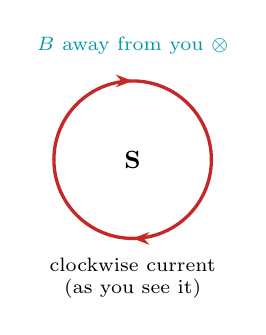
\begin{tikzpicture}
\draw[emred,very thick,postaction={decorate},decoration={markings,mark=at position 0.25 with {\arrowreversed{Stealth[length=6pt]}},mark=at position 0.75 with {\arrowreversed{Stealth[length=6pt]}}}] (0,0) circle (1);
\node[font=\small\bfseries] at (0,0) {S};
\node[font=\scriptsize,align=center] at (0,-1.5) {clockwise current\\(as you see it)};
\node[font=\scriptsize,align=center,fieldc] at (0,1.45) {$B$ away from you $\otimes$};
\end{tikzpicture}
\column{0.38\textwidth}\centering
\figlab{coil_hand.png}{width=0.52\linewidth}{
\draw[fptr] (1.08,0.95) node[flab,anchor=west]{thumb: $B$} -- (0.70,0.97);
\draw[fptr] (-0.08,0.45) node[flab,anchor=east,align=right]{fingers:\\current $I$} -- (0.12,0.70);}\\
{\scriptsize fig-5(b): right hand rule for a coil}
\begin{examtip}
\small Memory aid: letters \textbf{N} and \textbf{S} drawn with arrows at their ends run anticlockwise and clockwise respectively.
\end{examtip}
\end{columns}
\end{frame}

% =====================================================================
\begin{frame}{10.3.3 Field of a solenoid (Activity 6) \hfill \badge{2M} \badge{4M}}
\begin{columns}[T]
\column{0.4\textwidth}\centering
\figlab{solenoid_setup.png}{height=0.26\textheight}{
\draw[fptr] (0.12,1.08) node[flab,anchor=south]{solenoid (long helix)} -- (0.36,0.84);
\draw[fptr] (0.70,-0.05) node[flab,anchor=north]{to current supply} -- (0.83,0.52);}\\[4pt]
{\scriptsize fig-6(a)}\\[8pt]
\figlab{solenoid_field.png}{height=0.27\textheight}{
\node[font=\small\bfseries,emred] at (-0.04,0.5) {N};
\node[font=\small\bfseries,emred] at (1.04,0.5) {S};
\node[font=\scriptsize\bfseries,emred] at (0.08,0.80) {$I$};
\node[font=\scriptsize\bfseries,emred] at (0.93,0.80) {$I$};
}\\[2pt]
{\scriptsize fig-6(b): field lines (iron filings)}
\column{0.58\textwidth}
\small
\begin{defn}[Solenoid]
\small A long wire wound in a \textbf{close-packed helix}.
\end{defn}
\begin{itemize}
\item Iron filings show a pattern like that of a \textbf{bar magnet}: a solenoid behaves like a bar magnet.
\item One end is N, the other S (find with the right hand rule).
\item Outside: field lines go \textbf{N $\to$ S}; inside: \textbf{S $\to$ N}, strong and nearly uniform (parallel lines).
\item Lines outside are continuous with those inside $\Rightarrow$ field lines are \imp{closed loops}. Same for a bar magnet.
\end{itemize}
\begin{answer}[Big idea]
\small Moving charges (currents) produce magnetic fields.
\end{answer}
\end{columns}
\end{frame}

% =====================================================================
\section{Part B: Magnetic force}
% =====================================================================
\begin{frame}{Part B: Fields push on currents}
\begin{goals}
\large\begin{itemize}
\item Find the \textbf{direction and size} of the force on a moving charge, $F=qvB\sin\theta$.
\item Show why a charge in a field moves in a \textbf{circle}: $r=mv/Bq$.
\item Derive $F=ILB\sin\theta$ for a current-carrying wire.
\item Explain how an \textbf{electric motor} keeps turning.
\end{itemize}
\end{goals}
\end{frame}

\begin{frame}{10.4 Force on a moving charge (Activity 7) \hfill \badge{1M} \badge{2M}}
\begin{columns}[T]
\column{0.52\textwidth}
\begin{activity}[Activity 7: magnet near an old CRT TV]
\small The picture gets \textbf{distorted}; move the magnet away and it clears.
\end{activity}
\small The picture is made by a beam of \textbf{moving electrons}. The magnetic field exerts a force on them and changes their path: the \key{magnetic force}.
\begin{formula}[Magnetic force on a charge]
\[F=qvB\quad(\vec v\perp\vec B)\qquad F=qvB\sin\theta\]
$\theta$ = angle between $\vec v$ and $\vec B$.
\end{formula}
\column{0.46\textwidth}\centering
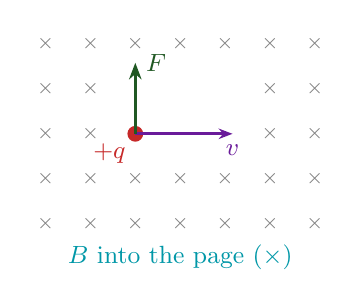
\begin{tikzpicture}[scale=0.95]
\foreach \x in {0,...,6}{\foreach \y in {0,...,4}{\node[font=\scriptsize,gray] at (\x*0.6,\y*0.6) {$\times$};}}
\fill[white] (0.9,0.95) rectangle (2.7,2.2);
\fill[emred] (1.2,1.2) circle (3pt) node[below left,font=\small]{$+q$};
\draw[vvec] (1.2,1.2) -- (2.5,1.2) node[below,font=\small]{$v$};
\draw[fvec] (1.2,1.2) -- (1.2,2.15) node[right,font=\small]{$F$};
\node[font=\small,fieldc] at (1.8,-0.45) {$B$ into the page ($\times$)};
\end{tikzpicture}\\
{\scriptsize fig-7: charge moving $\perp$ to $B$}
\begin{tcolorbox}[colback=emblue!4,colframe=emblue,title={\textbf{Special cases of $F=qvB\sin\theta$}}]
\small $\theta=90^\circ$: $F=qvB$ (maximum)\\
$\theta=0^\circ$ or $180^\circ$ (moving along or against $B$): $\sin\theta=0\Rightarrow$ \imp{$F=0$}\\
$v=0$ (charge at rest): $F=0$
\end{tcolorbox}
\end{columns}
\end{frame}

% =====================================================================
\begin{frame}[shrink=6]{Direction of the magnetic force: right hand rules \hfill \badge{1M} \badge{2M}}
\begin{columns}[T]
\column{0.48\textwidth}\centering
\figlab{rh_rule_a.png}{height=0.42\textheight}{
\node[font=\small\bfseries,emgreen!60!black,anchor=south] at (0.21,1.0) {$F$ (thumb)};
\node[font=\small\bfseries,fieldc,anchor=west] at (0.90,0.47) {$B$};
\node[font=\small\bfseries,empurple,anchor=west] at (0.84,0.06) {$v$};}\\
{\scriptsize fig-8(a): fingers along $v$, curl towards $B$; thumb gives $F$}
\column{0.5\textwidth}\centering
\figlab{rh_rule_b.png}{height=0.42\textheight}{
\node[font=\small\bfseries,emgreen!60!black,anchor=south] at (0.83,1.0) {$F$ (thumb)};
\node[font=\small\bfseries,empurple,anchor=south] at (0.12,0.55) {forefinger: $v$ or $I$};
\node[font=\scriptsize\bfseries,fieldc,anchor=north,align=center] at (0.55,0.0) {middle finger: $B$ (out of paper)};}\\[8pt]
{\scriptsize fig-8(b): three fingers mutually perpendicular}
\end{columns}
\vspace{2pt}
\begin{examtip}
\small $F$ is always \textbf{perpendicular to both} $v$ and $B$. Rules are for a \textbf{positive} charge; for a \textbf{negative} charge (electron) find the direction for $+q$, then \textbf{reverse} it.
\end{examtip}
\end{frame}

% =====================================================================
\begin{frame}[shrink=6]{Derivation 2: circular path of a charge, $r=\dfrac{mv}{Bq}$, $T=\dfrac{2\pi m}{Bq}$ \hfill \badge{4M}}
\begin{columns}[T]
\column{0.36\textwidth}\centering
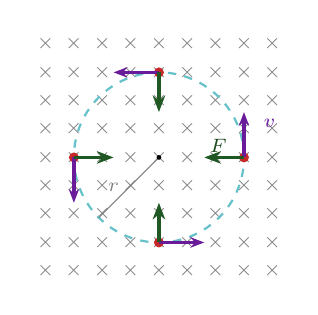
\begin{tikzpicture}[scale=0.72]
\xgrid{-4}{4}{-4}{4}
\draw[fieldc!60,dashed,thick] (0,0) circle (1.5);
\foreach \a in {0,90,180,270}{
  \coordinate (P) at (\a:1.5);
  \fill[emred] (P) circle (2.5pt);
  \draw[vvec] (P) -- ($(P)+(\a+90:0.8)$);
  \draw[fvec] (P) -- ($(P)+(\a+180:0.7)$);}
\node[font=\scriptsize,empurple] at (1.95,0.6) {$v$};
\node[font=\scriptsize,emgreen!60!black] at (1.05,0.2) {$F$};
\draw[gray] (0,0) -- (-1.06,-1.06) node[midway,left,font=\scriptsize]{$r$};
\fill (0,0) circle (1.2pt);
\end{tikzpicture}\\
{\scriptsize fig-E-1: $F\perp v$ always, towards the centre}
\column{0.62\textwidth}
\begin{steps}[3.6cm]
\stp1 & F=qvB & $v\perp B$, so $\sin90^\circ=1$\\
\stp2 & F\perp v & force never changes the speed, only the direction $\Rightarrow$ uniform circular motion\\
\stp3 & \frac{mv^2}{r}=qvB & magnetic force supplies the centripetal force\\
\stp4 & r=\frac{mv}{Bq} & multiply by $r$, cancel one $v$, divide by $qB$\\
\stp5 & T=\frac{2\pi r}{v} & time = circumference $\div$ speed\\
\stp6 & T=\frac{2\pi}{v}\cdot\frac{mv}{Bq}=\frac{2\pi m}{Bq} & substitute $r$; $v$ cancels\\
\end{steps}
\end{columns}
{\small\textbf{Note:} $T$ does \textbf{not} depend on speed: a faster particle moves in a bigger circle in the same time.}
\end{frame}

% =====================================================================
\begin{frame}{Solved numericals: force on a moving charge \hfill \badge{2M}}
\small
\begin{columns}[T]
\column{0.5\textwidth}
\begin{tcolorbox}[colback=emblue!4,colframe=emblue,title={\textbf{Q1.} A proton ($1.6\times10^{-19}$ C) moves at $2\times10^6$ m/s $\perp$ to $B=0.5$ T. Find $F$.}]
\stp1 $F=qvB$ \;($\theta=90^\circ$)\\
\stp2 $F=1.6\times10^{-19}\times2\times10^6\times0.5$\\
\stp3 $F=\boxed{1.6\times10^{-13}\ \text{N}}$
\end{tcolorbox}
\pause
\begin{tcolorbox}[colback=emblue!4,colframe=emblue,title={\textbf{Q2.} Same proton moves at $30^\circ$ to $B$.}]
\stp1 $F=qvB\sin30^\circ=1.6\times10^{-13}\times\frac12$\\
\stp2 $F=\boxed{8\times10^{-14}\ \text{N}}$
\end{tcolorbox}
\column{0.5\textwidth}
\pause
\begin{tcolorbox}[colback=emgreen!5,colframe=emgreen,title={\textbf{Q3.} Electron ($m=9.1\times10^{-31}$ kg) at $10^6$ m/s $\perp$ to $B=10^{-3}$ T. Radius?}]
\stp1 $r=\dfrac{mv}{Bq}=\dfrac{9.1\times10^{-31}\times10^6}{10^{-3}\times1.6\times10^{-19}}$\\[3pt]
\stp2 $=\dfrac{9.1\times10^{-25}}{1.6\times10^{-22}}=\boxed{5.7\times10^{-3}\ \text{m}}\approx5.7$ mm
\end{tcolorbox}
\pause
\begin{think}
\small A charge moves parallel to $B$. Force?\\
\onslide<5->{\textbf{Zero}, since $\sin0^\circ=0$.}
\end{think}
\end{columns}
\end{frame}

% =====================================================================
\begin{frame}[shrink=6]{Derivation 3: force on a current-carrying wire, $F=ILB$ \hfill \badge{4M}}
\begin{columns}[T]
\column{0.34\textwidth}\centering
\begin{tikzpicture}[scale=0.7]
\fill[fieldc!8] (-1.25,-1.5) rectangle (1.25,1.5);
\xgrid{-2}{2}{-2}{2}
\draw[line width=2.5pt] (0,-2.4) -- (0,2.4);
\draw[cur] (0.3,-0.4) -- (0.3,0.8) node[right,font=\small]{$I$};
\draw[fvec] (-0.1,0) -- (-1.4,0) node[left,font=\small]{$F$};
\draw[{Stealth}-{Stealth},gray] (1.55,-1.5) -- (1.55,1.5) node[midway,right,font=\small,black]{$L$};
\node[font=\small,fieldc] at (-0.9,1.9) {$B\ (\times)$};
\end{tikzpicture}\\
{\scriptsize fig-9: only length $L$ lies in the field}\\[4pt]
\begin{examtip}
\scriptsize $\parallel B$: $F=0$.\; $\perp B$: $F=ILB$ (max). In fig-9 the force on the upward current is to the \textbf{left} (right hand rule).
\end{examtip}
\column{0.64\textwidth}
\begin{steps}[3.0cm]
\stp1 & F_0=qvB & force on one charge moving with drift velocity $v$ $\perp B$\\
\stp2 & F=QvB\;\cdots(1) & add up for the total charge $Q$ inside the field\\
\stp3 & t=\frac{L}{v}\Rightarrow v=\frac{L}{t}\;\cdots(2) & time for the charge to cross the length $L$\\
\stp4 & F=\frac{QLB}{t}=\frac{Q}{t}LB\;\cdots(3) & put (2) in (1)\\
\stp5 & I=\frac{Q}{t} & definition of current\\
\stp6 & F=ILB\;\cdots(4) & put step 5 in (3)\\
\stp7 & F=ILB\sin\theta\;\cdots(5) & $\theta$ = angle between current and field\\
\end{steps}
\end{columns}
\end{frame}

% =====================================================================
\begin{frame}{Activity 8: wire in a horseshoe magnet \hfill \badge{4M: experiment}}
\begin{columns}[T]
\column{0.5\textwidth}\centering
\figlab{wire_force_setup.png}{width=0.8\linewidth}{
\draw[fptr] (0.60,1.10) node[flab,anchor=south]{horseshoe magnet} -- (0.50,0.93);
\draw[fptr] (0.10,1.10) node[flab,anchor=south]{copper wire} -- (0.30,0.86);
\draw[fptr] (0.36,0.62) node[flab,anchor=east]{force $F$} -- (0.48,0.62);
\draw[fptr] (0.05,0.42) node[flab,anchor=east]{wooden stick} -- (0.23,0.45);
\draw[fptr] (0.35,0.05) node[flab,anchor=north]{9 V battery} -- (0.44,0.38);
\draw[fptr] (0.66,0.05) node[flab,anchor=north]{switch} -- (0.52,0.36);
\draw[fptr] (0.85,-0.12) node[flab,anchor=north]{wooden plank} -- (0.88,0.22);}\\[14pt]
{\scriptsize fig-10}
\column{0.46\textwidth}
\small
\begin{enumerate}
\item Stretch a copper wire between two split sticks; connect to a 9 V battery and switch.
\item Switch on and bring a horseshoe magnet around the wire.
\item The wire is \textbf{deflected}; the direction agrees with the right hand rule.
\item Reverse the magnet's poles, or reverse the current: the deflection \textbf{reverses}.
\end{enumerate}
\begin{answer}[Conclusion]
\small A current-carrying wire in a magnetic field experiences a force; its direction depends on the directions of the current and of the field.
\end{answer}
\end{columns}
\end{frame}

% =====================================================================
\begin{frame}{Why does the wire move? Combining the fields \hfill \badge{2M} \badge{4M}}
\begin{columns}[c]
\column{0.24\textwidth}\centering
\begin{tikzpicture}[scale=0.7]
\foreach \y in {-1.2,-0.6,0,0.6,1.2} \draw[fl=0.55] (-1.4,\y) -- (1.4,\y);
\node[font=\small\bfseries] at (-1.7,0) {N}; \node[font=\small\bfseries] at (1.7,0) {S};
\end{tikzpicture}\\{\scriptsize (a) magnet's field}
\column{0.24\textwidth}\centering
\begin{tikzpicture}[scale=0.7]
\foreach \r in {0.45,0.9,1.35} \draw[fieldc,thick,postaction={decorate},decoration={markings,mark=at position 0.25 with {\arrowreversed{Stealth[length=4pt]}},mark=at position 0.75 with {\arrowreversed{Stealth[length=4pt]}}}] (0,0) circle (\r);
\inpage{(0,0)}
\end{tikzpicture}\\{\scriptsize (b) wire, current into page (clockwise)}
\column{0.24\textwidth}\centering
\figlab{combined_field.png}{width=0.85\linewidth}{
\node[flab,anchor=south] at (0.5,1.0) {strong (fields add)};
\node[flab,anchor=north] at (0.5,0.0) {weak (fields oppose)};
\draw[fvec] (0.5,0.46) -- (0.5,0.20);}\\[8pt]{\scriptsize (c) resultant: wire pushed to weak side}
\column{0.26\textwidth}
\small
\begin{itemize}
\item Above the wire, its clockwise field points \textbf{with} the magnet's field: strong.
\item Below, it points \textbf{against}: weak.
\item The non-uniform field pushes the wire from the strong to the \textbf{weak} region.
\end{itemize}
\end{columns}
\vspace{2pt}
{\scriptsize Check with the rule: $I$ into page, $B$ left to right $\Rightarrow F$ downward. \;fig-11(a),(b),(c)}
\end{frame}

% =====================================================================
\begin{frame}{Solved numericals: force on a wire \hfill \badge{2M}}
\small
\begin{columns}[T]
\column{0.5\textwidth}
\begin{tcolorbox}[colback=emblue!4,colframe=emblue,title={\textbf{Textbook App.\ Q4.} $F=8$ N on a 20 cm conductor $\perp$ to $B$, $I=40$ A. Find $B$.}]
\stp1 $L=20$ cm $=0.2$ m\\
\stp2 $F=ILB\Rightarrow B=\dfrac{F}{IL}$\\[2pt]
\stp3 $B=\dfrac{8}{40\times0.2}=\dfrac{8}{8}=\boxed{1\ \text{T}}$
\end{tcolorbox}
\pause
\begin{tcolorbox}[colback=emblue!4,colframe=emblue,title={\textbf{Q2.} $I=5$ A, $L=0.5$ m, $B=0.2$ T, wire at $30^\circ$ to $B$.}]
\stp1 $F=ILB\sin30^\circ=5\times0.5\times0.2\times\frac12=\boxed{0.25\ \text{N}}$
\end{tcolorbox}
\column{0.5\textwidth}
\pause
\begin{tcolorbox}[colback=emgreen!5,colframe=emgreen,title={\textbf{Textbook App.\ Q3 (fig-Q5).} Wire along its length, current $i$ upward, $B$ into page, length $L$ in field.}]
\begin{minipage}{0.3\linewidth}\centering
\begin{tikzpicture}[scale=0.55]
\xgrid{-2}{2}{-1}{1}
\draw[line width=2pt] (0,-1.2) -- (0,1.6);
\draw[cur] (0.3,0.3) -- (0.3,1.4) node[right,font=\scriptsize]{$i$};
\end{tikzpicture}
\end{minipage}\hfill
\begin{minipage}{0.66\linewidth}
\stp1 $\theta=90^\circ\Rightarrow F=iLB$\\
\stp2 Right hand rule: forefinger up ($i$), middle finger into page ($B$) $\Rightarrow$ thumb points \textbf{to the left}.
\end{minipage}
\end{tcolorbox}
\pause
\begin{think}
\small Force on a wire kept \textbf{parallel} to $B$?\\
\onslide<5->{\textbf{Zero}: every charge moves along the field.}
\end{think}
\end{columns}
\end{frame}

% =====================================================================
\begin{frame}{Motor in simple words}
\begin{simple}[Three ideas, in order]
\begin{enumerate}
\item A wire carrying current inside a magnetic field gets \textbf{pushed} sideways.
\item A coil has two long sides with currents in \textbf{opposite} directions, so one side is pushed \textbf{up} and the other \textbf{down}: the coil \textbf{spins}.
\item After half a turn the pushes would stop the spin. The \textbf{split ring (commutator)} reverses the current at that moment, so the coil keeps turning the same way.
\end{enumerate}
\end{simple}
\begin{examtip}[Pedal analogy]
Cycling: push down with one foot, then the other. The commutator is you switching feet at exactly the right time.
\end{examtip}
\end{frame}

% =====================================================================
\begin{frame}[shrink=6]{10.4.1 Electric motor: forces on a coil \hfill \badge{4M}}
\begin{columns}[c]
\column{0.44\textwidth}\centering
\begin{tikzpicture}[scale=0.9]
\foreach \y in {-1.6,-0.8,0,0.8,1.6} \draw[fl=0.08] (-2.6,\y) -- (2.6,\y);
\node[font=\small\bfseries,fieldc] at (2.6,2.0) {$B$};
\coordinate (A) at (-1,-1.2); \coordinate (Bc) at (-1,1.2); \coordinate (C) at (1,1.2); \coordinate (D) at (1,-1.2);
\draw[emred,line width=2pt] (A) -- (Bc) -- (C) -- (D) -- cycle;
\draw[cur] (-1.25,-0.5) -- (-1.25,0.5); \draw[cur] (1.25,0.5) -- (1.25,-0.5);
\node[below left,font=\small\bfseries] at (A) {A}; \node[above left,font=\small\bfseries] at (Bc) {B};
\node[above right,font=\small\bfseries] at (C) {C}; \node[below right,font=\small\bfseries] at (D) {D};
\inpage[0.16]{(-1.9,0.3)} \node[font=\scriptsize,emgreen!60!black] at (-1.9,-0.2) {$F$};
\outpage[0.16]{(1.9,0.3)} \node[font=\scriptsize,emgreen!60!black] at (1.9,-0.2) {$F$};
\end{tikzpicture}\\
{\scriptsize fig-12(a): current A$\to$B$\to$C$\to$D; $F$ on AB into page, on CD out of page}
\column{0.54\textwidth}
\small
\begin{enumerate}
\item AB and CD are always \textbf{perpendicular} to $B$ $\Rightarrow$ force $ILB$ on each.
\item Right hand rule: on AB (current up) force \textbf{into} the page; on CD (current down) force \textbf{out of} the page.
\item BC and DA: force zero when parallel to $B$; otherwise equal and opposite (up on BC, down on DA).
\item Forces on AB and CD: equal, opposite (equal currents in opposite directions) $\Rightarrow$ \imp{net force = 0}.
\item But they act along \textbf{different lines} $\Rightarrow$ they form a \key{couple} and \textbf{rotate} the coil, like two hands opening a bottle cap.
\end{enumerate}
\end{columns}
\end{frame}

% =====================================================================
\begin{frame}[shrink=6]{Electric motor: continuous rotation \hfill \badge{4M} \badge{Diagram}}
\begin{columns}[T]
\column{0.44\textwidth}\centering
\figlab{motor.png}{height=0.6\textheight}{
\node[font=\small\bfseries,emred] at (0.18,0.94) {N};
\node[font=\small\bfseries,emred] at (0.86,0.95) {S};
\draw[fptr] (0.55,1.05) node[flab,anchor=south]{coil ABCD, rotation axis} -- (0.58,0.84);
\draw[fptr] (-0.12,0.52) node[flab,anchor=east,align=right]{split rings\\C$_1$, C$_2$} -- (0.30,0.38);
\draw[fptr] (-0.12,0.52) -- (0.46,0.40);
\draw[fptr] (-0.12,0.30) node[flab,anchor=east,align=right]{brushes\\B$_1$, B$_2$} -- (0.12,0.37);
\draw[fptr] (-0.12,0.30) -- (0.58,0.30);
\node[font=\scriptsize\bfseries] at (0.13,0.00) {$+$};
\node[font=\scriptsize\bfseries] at (0.40,-0.02) {$-$};
\node[flab,anchor=north] at (0.27,-0.05) {battery};}\\[10pt]
{\scriptsize fig-12(c): simple electric motor}
\column{0.54\textwidth}
\footnotesize
\begin{itemize}
\item Without reversal: the coil turns to the vertical, overshoots by inertia, then the forces turn it \textbf{back}; it rocks to and fro.
\item \textbf{Fix:} reverse the current in the coil \textbf{every half rotation}.
\item The coil ends go to rings C$_1$, C$_2$ that rotate with it; fixed brushes B$_1$, B$_2$ connect to the battery.
\item After each half turn the rings swap brushes $\Rightarrow$ current in the coil reverses $\Rightarrow$ rotation continues in the \textbf{same direction}.
\end{itemize}
\begin{answer}[Energy]
\small Motor: \imp{electrical energy $\to$ mechanical energy}.
\end{answer}
\begin{tcolorbox}[colback=emteal!6,colframe=emteal,title={\textbf{Do you know? Fleming's left hand rule}}]
\scriptsize Stretch left-hand thumb, forefinger and middle finger mutually perpendicular: \textbf{forefinger} = field, \textbf{middle finger} = current, \textbf{thumb} = force (motion).
\end{tcolorbox}
\end{columns}
\end{frame}

% =====================================================================
\section{Part C: Electromagnetic induction}
% =====================================================================
\begin{frame}{Part C: Changing fields make currents}
\begin{goals}
\large\begin{itemize}
\item Explain \textbf{electromagnetic induction} with the magnet-and-coil activity.
\item State \textbf{Faraday's law} and \textbf{Lenz's law} and apply them.
\item Derive the motional emf $\varepsilon=Blv$.
\item Explain how \textbf{AC and DC generators} and magnetic levitation work.
\end{itemize}
\end{goals}
\end{frame}

\begin{frame}[shrink=6]{10.5 Electromagnetic induction (Activity 9) \hfill \badge{2M} \badge{4M}}
\begin{columns}[T]
\column{0.44\textwidth}\centering
\figlab{induction_setup.png}{width=0.82\linewidth}{
\node[font=\small\bfseries,emred] at (0.50,0.67) {N};
\draw[fptr] (0.62,1.08) node[flab,anchor=south]{bar magnet pushed in} -- (0.78,0.92);
\draw[fptr] (0.10,1.00) node[flab,anchor=south]{coil} -- (0.27,0.80);
\draw[fptr] (0.30,-0.08) node[flab,anchor=north]{galvanometer G} -- (0.11,0.07);}\\[12pt]
{\scriptsize fig-13}
\column{0.54\textwidth}
\footnotesize
\renewcommand{\arraystretch}{1.0}
\begin{tabular}{@{}p{3.3cm}p{2.6cm}@{}}
\toprule
\textbf{What we do} & \textbf{Galvanometer}\\
\midrule
Magnet at rest near coil & no deflection\\
N pole moved \textbf{towards} coil & deflects one way\\
N pole moved \textbf{away} & deflects the \textbf{other} way\\
S pole used instead & deflections reversed\\
Coil moved, magnet fixed & also deflects\\
\bottomrule
\end{tabular}
\begin{defn}[Electromagnetic induction]
\small Producing a current in a coil by \textbf{relative motion} between the coil and a magnet (changing flux). The current is the \key{induced current}; it is driven by an \key{induced emf}.
\end{defn}
\end{columns}
\end{frame}

% =====================================================================
\begin{frame}{Induction in simple words: only \emph{change} counts}
\begin{simple}[Key idea]
A magnet sitting still inside a coil makes \textbf{no} current, however strong it is. A magnet that is \textbf{moving} (or a field that is changing) makes a current.
\end{simple}
\begin{itemize}
\item \textbf{Faster} movement $\Rightarrow$ \textbf{larger} induced emf.
\item \textbf{More turns} in the coil $\Rightarrow$ larger induced emf.
\item \textbf{Stronger} magnet $\Rightarrow$ larger induced emf.
\item Reverse the motion $\Rightarrow$ the current flows the \textbf{opposite} way.
\end{itemize}
\end{frame}

% =====================================================================
\begin{frame}{10.5.1 Faraday's law \hfill \badge{1M} \badge{2M} \badge{4M}}
\begin{columns}[T]
\column{0.55\textwidth}
\begin{defn}[Faraday's law (first form)]
\small Whenever there is a \textbf{continuous change of magnetic flux} linked with a closed coil, a current is generated in the coil.
\end{defn}
\begin{defn}[Faraday's law of induction]
\small The induced emf in a closed loop \textbf{equals the rate of change of magnetic flux} through it.
\end{defn}
\small Faster change of flux $\Rightarrow$ greater induced emf.
\column{0.43\textwidth}
\begin{formula}
\[\varepsilon=\frac{\Delta\Phi}{\Delta t}\;\cdots(6)\]
Coil of $N$ turns, flux $\Phi_0$ per turn:
\[\Phi=N\Phi_0\;\cdots(7)\qquad\varepsilon=N\frac{\Delta\Phi_0}{\Delta t}\]
\end{formula}
\begin{examtip}
\small No change of flux $\Rightarrow$ no emf, however strong the field.
\end{examtip}
\end{columns}
\end{frame}

% =====================================================================
\begin{frame}{Lenz's law in simple words: nature resists change}
\begin{simple}[Think of a heavy door]
Push a heavy door and you \textbf{feel it push back}. The coil does the same: when you push a magnet in, the induced current makes the coil push \textbf{back}.
\end{simple}
\begin{itemize}
\item Induced current \textbf{always opposes} what causes it.
\item Magnet approaching $\Rightarrow$ coil face becomes the \textbf{same pole} (repels).
\item Magnet leaving $\Rightarrow$ coil face becomes the \textbf{opposite} pole (attracts).
\end{itemize}
\begin{examtip}[Why must it oppose?]
If it helped the motion, the magnet would speed up by itself and give free energy forever. That breaks \textbf{conservation of energy}.
\end{examtip}
\end{frame}

% =====================================================================
\begin{frame}{10.5.2 Lenz's law: the direction of the induced current \hfill \badge{2M} \badge{4M}}
\begin{columns}[T]
\column{0.44\textwidth}\centering
\figlab{lenz.png}{width=0.95\linewidth}{
\node[font=\small\bfseries,emred] at (0.44,0.50) {N};
\node[font=\small\bfseries,emred] at (0.97,0.50) {S};
\draw[fptr] (0.36,1.08) node[flab,anchor=south]{coil face near magnet becomes N} -- (0.20,0.86);
\draw[fptr] (0.62,0.08) node[flab,anchor=north]{magnet pushed towards coil} -- (0.55,0.33);
\node[flab,anchor=east] at (0.14,0.52) {coil};}\\[12pt]
{\scriptsize fig-14: N faces N $\Rightarrow$ the coil repels the magnet}
\column{0.54\textwidth}
\small
\textbf{Reasoning (conservation of energy):}
\begin{enumerate}
\item Suppose the induced current made the coil's near face \textbf{S}. It would \textbf{attract} the approaching N pole; the magnet would speed up and gain kinetic energy \textbf{from nothing}, and electrical energy would also appear. Impossible.
\item So the near face must be \textbf{N}: it \textbf{repels} the magnet. We must do work to push it; that work becomes electrical energy.
\item Pulling the magnet away: the near face becomes \textbf{S} and attracts, again opposing the motion.
\end{enumerate}
\begin{defn}[Lenz's law]
\small The induced current flows in a direction that \textbf{opposes the change in flux} that produces it.
\end{defn}
\end{columns}
\end{frame}

% =====================================================================
\begin{frame}[shrink=6]{10.5.3 Derivation 4, part 1: the set-up \hfill \badge{4M}}
\begin{columns}[T]
\column{0.5\textwidth}\centering
\figlab{crosswire.png}{width=0.95\linewidth}{
\node[font=\small\bfseries,emred] at (0.36,0.93) {N};
\node[font=\small\bfseries,emred] at (0.36,0.38) {S};
\draw[fptr] (0.55,1.07) node[flab,anchor=south]{distance $s$} -- (0.64,0.85);
\node[flab] at (0.975,0.53) {$l$};
\draw[fptr] (0.97,1.07) node[flab,anchor=south]{parallel conductors} -- (0.88,0.68);
\draw[fptr] (0.70,0.12) node[flab,anchor=north]{cross wire} -- (0.50,0.62);
\draw[fptr] (0.08,0.98) node[flab,anchor=south]{induced current} -- (0.10,0.72);
\draw[fptr] (0.05,0.05) node[flab,anchor=north]{galvanometer} -- (0.10,0.30);
\node[flab] at (0.45,0.52) {$B$ (downwards)};}\\[10pt]
{\scriptsize fig-15}
\column{0.48\textwidth}
\small
\begin{itemize}
\item Two parallel bare conductors, $l$ metres apart, in a uniform field $B$ (perpendicular to their plane), joined through a galvanometer.
\item A bare \textbf{cross wire} rests across them, closing the loop.
\item Move the cross wire to the \textbf{left}: needle deflects one way. To the \textbf{right}: the other way.
\item It moves a distance $s$ in time $\Delta t$, with speed $v=\dfrac{s}{\Delta t}$.
\item A current $I$ flows $\Rightarrow$ there is an emf $\varepsilon$. By \textbf{conservation of energy}, the electrical energy comes from the work we do in moving the wire (friction ignored).
\end{itemize}
\end{columns}
\end{frame}

\begin{frame}[shrink=6]{Derivation 4, part 2: work done equals flux change $\times$ current \hfill \badge{4M}}
\begin{columns}[T]
\column{0.33\textwidth}\centering
\begin{tikzpicture}[scale=0.72]
\fill[fieldc!8] (-0.5,-0.3) rectangle (4.2,2.3);
\foreach \x in {0,...,8}{\foreach \y in {0,...,4}{\node[font=\tiny,gray] at (\x*0.5-0.25,\y*0.5) {$\times$};}}
\draw[very thick] (-0.5,0) -- (4.2,0); \draw[very thick] (-0.5,2) -- (4.2,2);
\draw[very thick] (4.2,0) -- (4.2,2);
\draw[emred,line width=2.5pt] (3,-0.2) -- (3,2.2);
\draw[emred,dashed,line width=1.5pt] (1.4,-0.2) -- (1.4,2.2);
\draw[-{Stealth},thick] (3,2.45) -- (1.4,2.45) node[midway,above,font=\scriptsize]{$s$ in time $\Delta t$};
\draw[{Stealth}-{Stealth},gray] (-0.75,0) -- (-0.75,2) node[midway,left,font=\small,black]{$l$};
\fill[emorange!40,opacity=0.5] (1.4,0) rectangle (3,2);
\node[font=\scriptsize,align=center] at (2.2,1) {area\\lost $=ls$};
\node[font=\scriptsize,fieldc] at (3.8,-0.55) {$B$ ($\perp$ plane)};
\end{tikzpicture}\\
{\scriptsize top view of the loop}
\column{0.66\textwidth}
\begin{steps}[5.2cm]
\stp1 & F=BIl\;\cdots(8) & field's force on current $I$ in length $l$ (eq.\ 4); opposes our push\\
\stp2 & W=Fs=BIls\;\cdots(9) & our work against it over distance $s$\\
\stp3 & \Delta\Phi=B\,(ls)\;\cdots(10) & loop area falls by $ls$; $B\perp$ area so $\Phi=BA$\\
\stp4 & W=(\Delta\Phi)\,I & compare (9) and (10): $Bls=\Delta\Phi$\\
\stp5 & \frac{W}{\Delta t}=\frac{I\,\Delta\Phi}{\Delta t}\;\cdots(11) & divide by $\Delta t$ (work per second)\\
\stp6 & P=\varepsilon I\;\cdots(12) & electric power = emf $\times$ current\\
\stp7 & \varepsilon=\frac{\Delta\Phi}{\Delta t} & compare (11), (12): \textbf{Faraday's law}\\
\end{steps}
\end{columns}
\end{frame}

\begin{frame}[shrink=6]{Derivation 4, part 3: motional emf, $\varepsilon=Blv$ \hfill \badge{4M}}
\begin{columns}[T]
\column{0.6\textwidth}
\begin{steps}[3.1cm]
\stp1 & \frac{W}{\Delta t}=\frac{Fs}{\Delta t}=\frac{BIls}{\Delta t}\;\cdots(13) & divide (9) by $\Delta t$\\
\stp2 & \frac{s}{\Delta t}=v & speed of the cross wire\\
\stp3 & P=Fv=BIlv\;\cdots(14) & power = force $\times$ velocity\\
\stp4 & \varepsilon I=BIlv & (12) and (14) are the same power\\
\stp5 & \varepsilon=Blv & cancel $I$ on both sides\\
\end{steps}
\begin{formula}[Motional emf]
\[\boxed{\varepsilon=Blv}\]
emf between the ends of a conductor of length $l$ moving with speed $v$ perpendicular to a uniform field $B$.
\end{formula}
\column{0.38\textwidth}
\begin{examtip}[Note]
\small $\varepsilon=Blv$ is \textbf{not} Faraday's law itself: it refers to a \textbf{single moving conductor}, not a loop. It is useful whenever a conductor moves in a uniform field.
\end{examtip}
\begin{tcolorbox}[colback=emblue!5,colframe=emblue,title={\textbf{Chain of equations}}]
\scriptsize (8) $F=BIl$ $\to$ (9) $W=BIls$\\
(10) $\Delta\Phi=Bls$ $\to$ $W=I\Delta\Phi$\\
(11) $\div\Delta t$, (12) $P=\varepsilon I$ $\to$ $\varepsilon=\frac{\Delta\Phi}{\Delta t}$\\
(13), (14) $P=Fv=BIlv$ $\to$ $\varepsilon=Blv$
\end{tcolorbox}
\end{columns}
\end{frame}

% =====================================================================
\begin{frame}[shrink=6]{Solved examples: induced emf \hfill \badge{2M} \badge{4M}}
\small
\begin{columns}[T]
\column{0.52\textwidth}
\begin{tcolorbox}[colback=emblue!4,colframe=emblue,title={\textbf{Example 1 (textbook).} Coil of 400 turns; flux per turn varies as in the graph.}]
\centering
\begin{tikzpicture}
\begin{axis}[width=5.6cm,height=3.2cm,axis lines=left,xmin=0,xmax=0.5,ymin=0,ymax=0.0012,
  xtick={0,0.1,0.2,0.3,0.4,0.5},ytick={0,0.0005,0.001},
  yticklabel style={/pgf/number format/fixed,/pgf/number format/precision=4,font=\tiny},
  xticklabel style={font=\tiny},xlabel={\scriptsize $t$ (s)},ylabel={\scriptsize $\Phi$ (Wb)},grid=major]
\addplot[emred,very thick] coordinates {(0,0)(0.1,0.001)(0.3,0.001)(0.4,0)};
\end{axis}
\end{tikzpicture}\\[-2pt]
\raggedright
\stp1 0 to 0.1 s: $\Delta\Phi_0=0.001$ Wb, $\Delta t=0.1$ s\\
\stp2 $\varepsilon=N\dfrac{\Delta\Phi_0}{\Delta t}=\dfrac{400\times0.001}{0.1}=\boxed{4\ \text{V}}$ (maximum)\\
\stp3 0.1 s to 0.3 s: flux constant $\Rightarrow\Delta\Phi=0\Rightarrow\varepsilon=\boxed{0}$
\end{tcolorbox}
\column{0.46\textwidth}
\pause
\begin{tcolorbox}[colback=emgreen!5,colframe=emgreen,title={\textbf{Example 2 (textbook).} $v=10$ m/s $\perp B=0.8$ T, $\varepsilon=8$ V. Find $l$.}]
\stp1 $\varepsilon=Blv\Rightarrow l=\dfrac{\varepsilon}{Bv}$\\[2pt]
\stp2 $l=\dfrac{8}{0.8\times10}=\boxed{1\ \text{m}}$
\end{tcolorbox}
\pause
\begin{tcolorbox}[colback=emblue!4,colframe=emblue,title={\textbf{Q3.} Flux through a 50-turn coil falls from $0.02$ Wb to 0 in $0.1$ s (per turn).}]
\stp1 $\varepsilon=N\dfrac{\Delta\Phi_0}{\Delta t}=\dfrac{50\times0.02}{0.1}=\boxed{10\ \text{V}}$
\end{tcolorbox}
\end{columns}
\end{frame}

% =====================================================================
\begin{frame}{10.5.4 Applications of electromagnetic induction \hfill \badge{2M} \badge{Textbook App.\ Q6}}
\begin{columns}[T]
\column{0.5\textwidth}
\begin{tcolorbox}[colback=emblue!5,colframe=emblue,title={\textbf{Security check (metal detector)}}]
\small People walk through a large coil carrying a weak AC field. Iron on the body changes the flux linked with the coil; the induced current \textbf{triggers an alarm}.
\end{tcolorbox}
\begin{tcolorbox}[colback=emblue!5,colframe=emblue,title={\textbf{Tape recorder}}]
\small Tape coated with iron oxide is magnetised unevenly. Moving past a small coil (the head), its changing field induces a current in the coil.
\end{tcolorbox}
\column{0.48\textwidth}
\begin{tcolorbox}[colback=emgreen!5,colframe=emgreen,title={\textbf{Induction stove}}]
\small A coil below the cooking surface carries AC $\Rightarrow$ alternating field. It induces an emf and current in the \textbf{metal pan}; the pan's resistance turns the current into \textbf{heat}, which heats the water.
\end{tcolorbox}
\begin{tcolorbox}[colback=emgreen!5,colframe=emgreen,title={\textbf{ATM card swipe}}]
\small The magnetic strip moves past a coil in the reader; the changing flux induces a current pattern that is read as the card's data.
\end{tcolorbox}
\end{columns}
\end{frame}

% =====================================================================
\begin{frame}{10.5.5 Magnetic levitation \hfill \badge{2M} \badge{4M}}
\begin{columns}[T]
\column{0.28\textwidth}\centering
\figlab{levitation.png}{height=0.55\textheight}{
\draw[fptr] (-0.15,1.02) node[flab,anchor=south west]{soft iron core} -- (0.40,0.95);
\draw[fptr] (-0.15,0.74) node[flab,anchor=east]{metal ring} -- (0.10,0.72);
\draw[fptr] (-0.15,0.50) node[flab,anchor=east]{coil} -- (0.22,0.50);
\draw[fptr] (0.80,-0.04) node[flab,anchor=north]{to AC supply} -- (0.93,0.29);
\draw[fptr] (-0.15,0.10) node[flab,anchor=east]{wooden base} -- (0.15,0.14);}\\
{\scriptsize fig-16(a)}
\column{0.24\textwidth}\centering
\begin{tikzpicture}[scale=0.75]
\draw[thick] (0,0) ellipse (1.1 and 0.3);
\draw[fvec] (0,0) -- (0,1.5) node[above,font=\small]{$F$};
\draw[-{Stealth[length=6pt]},emred,very thick] (0,0) -- (0,-1.5) node[below,font=\small]{$W$};
\end{tikzpicture}\\
{\scriptsize fig-16(b): $F=W$}
\column{0.46\textwidth}
\small
\begin{enumerate}
\item AC through the coil: the ring \textbf{floats}. Switch off: the ring jumps up.
\item Ring at rest $\Rightarrow$ net force 0 (Newton's 2nd law): an upward force $F$ balances the weight $W$.
\item AC keeps reversing $\Rightarrow$ the coil's poles reverse $\Rightarrow$ the flux through the ring keeps changing $\Rightarrow$ induced current in the ring.
\item By Lenz's law the ring's face is \textbf{like} the coil's top face (coil top S, ring bottom S) $\Rightarrow$ \textbf{repulsion} lifts the ring.
\item With \textbf{DC} the ring jumps only at switch on/off (flux changes only then) and falls back.
\end{enumerate}
\end{columns}
\end{frame}

\begin{frame}[shrink=8]{Levitation: why is the ring repelled? \hfill \badge{2M}}
\begin{columns}[c]
\column{0.46\textwidth}\centering
\figlab{levitation_field.png}{width=0.9\linewidth}{
\draw[fptr] (0.80,0.93) node[flab]{ring (induced current)} -- (0.80,0.66);
\draw[fptr] (0.45,0.30) node[flab]{coil} -- (0.63,0.25);
\draw[fptr] (0.12,0.62) node[flab,anchor=south]{AC source} -- (0.13,0.37);
\node[flab] at (0.30,0.93) {field lines of coil};}\\[4pt]
{\scriptsize fig-16(c)}
\column{0.52\textwidth}
\small
\begin{steps}[3.2cm]
\stp1 & \text{AC in coil} & current changes size and direction continuously\\
\stp2 & \text{flux through ring changes} & ring area fixed, field through it changes\\
\stp3 & \text{induced current in ring} & Faraday's law\\
\stp4 & \text{ring opposes the change} & Lenz's law: ring's lower face is like the coil's upper face\\
\stp5 & \text{repulsion}=W & upward force balances weight: ring floats\\
\end{steps}
\end{columns}
\end{frame}

% =====================================================================
\begin{frame}{Generator in simple words: a motor run backwards}
\begin{columns}[c]
\column{0.48\textwidth}
\begin{tcolorbox}[colback=emorange!8,colframe=emorange,title={\faCog\ Motor}]
\centering \textbf{Electrical energy} $\longrightarrow$ \textbf{motion}\\ current pushes the coil
\end{tcolorbox}
\column{0.48\textwidth}
\begin{tcolorbox}[colback=emgreen!8,colframe=emgreen,title={\faBolt\ Generator}]
\centering \textbf{Motion} $\longrightarrow$ \textbf{electrical energy}\\ we spin the coil, current appears
\end{tcolorbox}
\end{columns}
\begin{simple}[Why it works]
Spinning the coil in a magnetic field keeps changing the flux through it, so an emf is induced (Faraday's law). Turn faster $\Rightarrow$ more emf.
\end{simple}
\end{frame}

% =====================================================================
\begin{frame}{10.5.6 AC generator \hfill \badge{4M} \badge{Diagram}}
\begin{columns}[T]
\column{0.38\textwidth}\centering
\figlab{ac_generator.png}{height=0.7\textheight}{
\node[font=\small\bfseries,emred] at (0.09,0.36) {N};
\node[font=\small\bfseries,emred] at (0.91,0.50) {S};
\draw[fptr] (0.55,1.06) node[flab,anchor=south]{rotation} -- (0.48,0.93);
\draw[fptr] (-0.08,0.80) node[flab,anchor=east]{coil (side A)} -- (0.62,0.66);
\draw[fptr] (-0.08,0.60) node[flab,anchor=east]{side B} -- (0.33,0.53);
\draw[fptr] (-0.08,0.35) node[flab,anchor=east]{slip rings} -- (0.60,0.28);
\draw[fptr] (1.08,0.05) node[flab,anchor=west]{brushes} -- (0.60,0.08);
\draw[fptr] (-0.08,0.15) node[flab,anchor=east]{load} -- (0.20,0.12);}\\
{\scriptsize fig-17(a)}
\column{0.6\textwidth}
\small
\begin{itemize}
\item A coil is rotated between the poles of a magnet; the \textbf{flux through it changes} continuously $\Rightarrow$ induced emf (Faraday).
\item Coil ends go to two \textbf{full slip rings}; carbon brushes press on them and take current to the load.
\end{itemize}
\centering
\begin{tikzpicture}
\begin{axis}[width=7.6cm,height=3.6cm,axis lines=middle,xmin=0,xmax=1.35,ymin=-1.3,ymax=1.4,
  xtick={0.25,0.5,0.75,1},xticklabels={$\frac14$,$\frac12$,$\frac34$,1},ytick=\empty,
  xlabel={\scriptsize rev.},ylabel={\scriptsize emf},every axis x label/.style={at={(1,0.5)},anchor=west},every axis y label/.style={at={(0,1)},anchor=south}]
\addplot[emred,very thick,domain=0:1.25,samples=100] {sin(deg(2*pi*x))};
\node[font=\tiny,anchor=west] at (axis cs:0.30,1.1) {max (coil horizontal)};
\node[font=\tiny,anchor=west] at (axis cs:0.80,-1.05) {max, reversed};
\end{axis}
\end{tikzpicture}\\
{\scriptsize fig-17(b): alternating emf over one rotation}
\end{columns}
\end{frame}

\begin{frame}[shrink=6]{Why does the emf vary? AC and the DC generator \hfill \badge{2M} \badge{4M}}
\begin{columns}[T]
\column{0.5\textwidth}
\small
\textbf{One rotation, step by step:}
\begin{enumerate}
\item Coil \textbf{vertical} (plane $\perp$ field): flux maximum but changing slowest $\Rightarrow$ \textbf{emf zero}.
\item First quarter: emf rises; coil \textbf{horizontal} (plane $\parallel$ field): flux changing fastest $\Rightarrow$ \textbf{emf maximum}.
\item Second quarter: emf falls to zero (vertical again, B on top).
\item Second half: same pattern but sides A and B have swapped places $\Rightarrow$ \textbf{emf reversed}.
\end{enumerate}
\begin{defn}[Alternating current (AC)]
\small Current whose direction reverses periodically; it has a \textbf{frequency}.
\end{defn}
{\small Generator: \imp{mechanical $\to$ electrical energy}.}
\column{0.48\textwidth}\centering
\figlab{dc_generator.png}{height=0.38\textheight}{
\node[font=\small\bfseries,emred] at (0.09,0.36) {N};
\node[font=\small\bfseries,emred] at (0.92,0.50) {S};
\draw[fptr] (1.08,0.38) node[flab,anchor=west,align=left]{split rings\\(commutator)} -- (0.66,0.28);
\draw[fptr] (0.20,0.10) node[flab,anchor=east]{brush} -- (0.46,0.22);
\draw[fptr] (1.08,0.05) node[flab,anchor=west]{load $R$} -- (0.80,0.08);}\\
{\scriptsize fig-17(c): DC generator}\\[2pt]
\begin{tikzpicture}
\begin{axis}[width=6.3cm,height=2.9cm,axis lines=middle,xmin=0,xmax=1.3,ymin=0,ymax=1.3,
  xtick={0.25,0.5,0.75,1},xticklabels={$\frac14$,$\frac12$,$\frac34$,1},ytick=\empty,
  xlabel={\scriptsize rev.},ylabel={\scriptsize emf},every axis x label/.style={at={(1,0)},anchor=west}]
\addplot[emgreen!70!black,very thick,domain=0:1.25,samples=100] {abs(sin(deg(2*pi*x)))};
\end{axis}
\end{tikzpicture}\\
{\scriptsize fig-17(d): with half slip rings the current in the load keeps one direction (DC)}
\end{columns}
\end{frame}

\begin{frame}{Motor vs generator \hfill \badge{2M}}
\centering\small
\renewcommand{\arraystretch}{1.45}
\begin{tabular}{>{\bfseries}p{3.2cm}p{4.9cm}p{4.9cm}}
\toprule
\rowcolor{emblue}\textcolor{white}{Feature} & \textcolor{white}{\textbf{Electric motor}} & \textcolor{white}{\textbf{Generator (dynamo)}}\\
\midrule
Energy change & electrical $\to$ mechanical & mechanical $\to$ electrical\\
Principle & force on a current-carrying coil in a field ($F=ILB$) & electromagnetic induction ($\varepsilon=\Delta\Phi/\Delta t$)\\
Input & current from a battery/supply & rotation of the coil\\
Output & rotation & induced current\\
Rings & split rings: reverse current every half turn & AC: full slip rings;\; DC: split rings\\
Hand rule & right hand rule / Fleming's left hand rule & Lenz's law gives the current direction\\
\bottomrule
\end{tabular}
\end{frame}

% =====================================================================
\section{Revision}

\begin{frame}{All derivations of this chapter at a glance \hfill \badge{Revise}}
\small\centering
\renewcommand{\arraystretch}{1.5}
\begin{tabular}{>{\bfseries}c p{3.8cm} p{5.3cm} p{2.8cm}}
\toprule
\rowcolor{emblue}\textcolor{white}{No.} & \textcolor{white}{\textbf{Result}} & \textcolor{white}{\textbf{Key idea}} & \textcolor{white}{\textbf{Uses}}\\
\midrule
1 & $\Phi=BA\cos\theta$ & effective area $\perp$ field is $A\cos\theta$ & $B=\Phi/A$\\
2 & $r=\frac{mv}{Bq}$,\; $T=\frac{2\pi m}{Bq}$ & magnetic force = centripetal force & $F=qvB$\\
3 & $F=ILB\sin\theta$ & add $qvB$ over all charges, $v=L/t$, $I=Q/t$ & $F=qvB$\\
4 & $\varepsilon=\frac{\Delta\Phi}{\Delta t}$,\; $\varepsilon=Blv$ & work done = electrical energy; $\Delta\Phi=Bls$; $P=\varepsilon I=Fv$ & $F=BIl$\\
\bottomrule
\end{tabular}
\end{frame}

\begin{frame}{Concept map}
\centering
\begin{tikzpicture}[
  every node/.style={font=\scriptsize,align=center,rounded corners=3pt,inner sep=3pt},
  main/.style={fill=emblue,text=white,font=\small\bfseries},
  a/.style={fill=emblue!15,draw=emblue},
  b/.style={fill=empurple!15,draw=empurple},
  c/.style={fill=emgreen!15,draw=emgreen},
  l/.style={-{Stealth},thick,gray}]
\node[main] (c) at (0,0) {Electro-\\magnetism};
\node[a] (o) at (-4.3,1.8) {Oersted:\\current $\to$ field};
\node[a] (f) at (-6.3,0.4) {Field lines, $\Phi$, $B=\Phi/A$\\$\Phi=BA\cos\theta$};
\node[a] (w) at (-4.4,-1.0) {wire: circles (thumb rule)\\coil, solenoid};
\node[b] (q) at (0,2.3) {$F=qvB\sin\theta$\\$r=\frac{mv}{Bq}$};
\node[b] (i) at (-1.2,-2.3) {$F=ILB\sin\theta$};
\node[b] (m) at (2.0,-2.4) {Motor\\elec. $\to$ mech.};
\node[c] (e) at (4.3,1.8) {Induction\\Faraday $\varepsilon=\frac{\Delta\Phi}{\Delta t}$};
\node[c] (lz) at (6.3,0.4) {Lenz: opposes\\the change};
\node[c] (bl) at (4.6,-0.9) {$\varepsilon=Blv$};
\node[c] (g) at (6.0,-2.3) {Generator AC/DC\\mech. $\to$ elec.};
\draw[l] (c)--(o); \draw[l] (o)--(f); \draw[l] (o)--(w); \draw[l] (c)--(q); \draw[l] (q)--(i); \draw[l] (i)--(m);
\draw[l] (c)--(e); \draw[l] (e)--(lz); \draw[l] (e)--(bl); \draw[l] (bl)--(g);
\end{tikzpicture}
\end{frame}

\begin{frame}{Formula sheet \hfill \badge{Must memorise}}
\small
\renewcommand{\arraystretch}{1.55}
\centering
\begin{tabular}{>{\bfseries}p{4.8cm}p{8cm}}
\toprule
\rowcolor{emred}\textcolor{white}{Quantity} & \textcolor{white}{\textbf{Formula / unit}}\\
\midrule
Magnetic flux density & $B=\dfrac{\Phi}{A}$;\quad tesla (T) = Wb/m$^2$ = N/(A m)\\
Magnetic flux & $\Phi=BA\cos\theta$;\quad weber (Wb)\\
Force on a moving charge & $F=qvB\sin\theta$ \;($=qvB$ when $v\perp B$)\\
Charge in a uniform field & $r=\dfrac{mv}{Bq}$;\quad $T=\dfrac{2\pi m}{Bq}$\\
Force on a current & $F=ILB\sin\theta$ \;($=ILB$ when $I\perp B$)\\
Faraday's law & $\varepsilon=\dfrac{\Delta\Phi}{\Delta t}$;\quad $N$ turns: $\varepsilon=N\dfrac{\Delta\Phi_0}{\Delta t}$\\
Motional emf & $\varepsilon=Blv$\\
\bottomrule
\end{tabular}
\end{frame}

\begin{frame}{What we have learnt (textbook summary)}
\small
\begin{itemize}
\item \textbf{Magnetic flux}: a measure of the number of field lines through an area.
\item \textbf{Magnetic flux density} $B$: flux through a plane perpendicular to the field $\div$ area of the plane.
\item A current-carrying wire produces a magnetic field.
\item $F=qvB\sin\theta$ and $F=ILB\sin\theta$.
\item In an electric \textbf{motor}, electrical energy is converted into mechanical energy.
\item Producing current by relative motion between a coil and a magnetic field is \textbf{electromagnetic induction}.
\item \textbf{Faraday's law}: induced emf in a closed loop = rate of change of magnetic flux through it.
\item \textbf{Lenz's law}: the induced current opposes the change in flux.
\item A conductor of length $l$ moving $\perp$ to $B$ with speed $v$ develops the \textbf{motional emf} $Blv$.
\item In \textbf{generators}, mechanical energy is converted into electrical energy.
\end{itemize}
\end{frame}

% =====================================================================
\section{Question Bank}

\begin{frame}{1-mark questions \hfill \badge{1M}}
\small
\begin{columns}[T]
\column{0.5\textwidth}
\begin{enumerate}
\item Who showed a current affects a compass? \onslide<2->{\textcolor{emgreen}{\textbf{Oersted}}}
\item SI unit of magnetic flux? \onslide<2->{\textcolor{emgreen}{\textbf{weber}}}
\item SI unit of flux density? \onslide<2->{\textcolor{emgreen}{\textbf{tesla (Wb/m$^2$)}}}
\item Shape of field lines of a straight wire? \onslide<2->{\textcolor{emgreen}{\textbf{concentric circles}}}
\item Flux through a plane parallel to $B$? \onslide<2->{\textcolor{emgreen}{\textbf{zero}}}
\item Force on a charge moving along $B$? \onslide<2->{\textcolor{emgreen}{\textbf{zero}}}
\item Device like a bar magnet made of coils? \onslide<2->{\textcolor{emgreen}{\textbf{solenoid}}}
\end{enumerate}
\column{0.5\textwidth}
\begin{enumerate}\setcounter{enumi}{7}
\item Energy change in a motor? \onslide<2->{\textcolor{emgreen}{\textbf{electrical $\to$ mechanical}}}
\item Part that reverses current in a motor? \onslide<2->{\textcolor{emgreen}{\textbf{split rings}}}
\item Law giving the direction of induced current? \onslide<2->{\textcolor{emgreen}{\textbf{Lenz's law}}}
\item Lenz's law follows from? \onslide<2->{\textcolor{emgreen}{\textbf{conservation of energy}}}
\item Formula for motional emf? \onslide<2->{\textcolor{emgreen}{\textbf{$\varepsilon=Blv$}}}
\item Stove based on induction? \onslide<2->{\textcolor{emgreen}{\textbf{induction stove}}}
\item Rings used in an AC generator? \onslide<2->{\textcolor{emgreen}{\textbf{full slip rings}}}
\end{enumerate}
\end{columns}
\end{frame}

\begin{frame}{Textbook MCQs \hfill \badge{1M}}
\small
\begin{columns}[T]
\column{0.5\textwidth}
\begin{enumerate}
\item Converts electrical energy into mechanical energy:\\ a) motor \; b) battery \; c) generator \; d) switch\\
\onslide<2->{\textcolor{emgreen}{\textbf{Answer: a}}}
\item Converts mechanical energy into electrical energy:\\ a) motor \; b) battery \; c) generator \; d) switch\\
\onslide<2->{\textcolor{emgreen}{\textbf{Answer: c}}}
\item Force on a wire placed perpendicular to a uniform field:\\ a) 0 \; b) $ILB$ \; c) $2ILB$ \; d) $ILB/2$\\
\onslide<2->{\textcolor{emgreen}{\textbf{Answer: b}} ($\sin90^\circ=1$)}
\end{enumerate}
\column{0.5\textwidth}
\begin{enumerate}\setcounter{enumi}{3}
\item One tesla =\\ a) N/C \; b) N/(A m) \; c) A/m \; d) N/(A s)\\
\onslide<3->{\textcolor{emgreen}{\textbf{Answer: b}} ($B=F/IL$)}
\item Unit of magnetic flux:\\ a) dyne \; b) oersted \; c) gauss \; d) weber\\
\onslide<3->{\textcolor{emgreen}{\textbf{Answer: d}}}
\item No force acts on a current-carrying conductor kept\\ a) parallel to the field \; b) perpendicular to the field \; c) in the field \; d) away from the field\\
\onslide<3->{\textcolor{emgreen}{\textbf{Answer: a}}}
\end{enumerate}
\end{columns}
\end{frame}

\begin{frame}{Reflections on concepts: figure questions \hfill \badge{1M} \badge{2M}}
\footnotesize
\begin{columns}[T]
\column{0.5\textwidth}
\begin{minipage}[t]{0.3\linewidth}\centering
\begin{tikzpicture}[scale=0.45]
\foreach \r in {0.8,1.4,2.0} \draw[thick,postaction={decorate},decoration={markings,mark=at position 0.0 with {\arrow{Stealth[length=4pt]}},mark=at position 0.5 with {\arrow{Stealth[length=4pt]}}}] (0,0) circle (\r);
\fill[magenta] (0,0) circle (0.4);
\end{tikzpicture}\\{\tiny fig-Q1}
\end{minipage}\hfill
\begin{minipage}[t]{0.66\linewidth}
\textbf{Q2.} Field lines as in fig-Q1 (anticlockwise). Direction of current?\\
\onslide<2->{\textcolor{emgreen}{Thumb rule: anticlockwise field $\Rightarrow$ current \textbf{out of the page} (towards the reader).}}
\end{minipage}\\[6pt]
\begin{minipage}[t]{0.3\linewidth}\centering
\begin{tikzpicture}[scale=0.5]
\draw[magenta,thick] (0,0) ellipse (0.4 and 1.4);
\fill[gray!60] (1.3,-0.2) rectangle (3.5,0.2); \node[font=\tiny] at (1.5,0) {N};
\draw[-{Stealth}] (3.0,0.6) -- (1.6,0.6);
\end{tikzpicture}\\{\tiny fig-Q2}
\end{minipage}\hfill
\begin{minipage}[t]{0.66\linewidth}
\textbf{Q3.} N pole moves towards the coil. What happens to the flux?\\
\onslide<3->{\textcolor{emgreen}{Flux through the coil \textbf{increases}; a current is induced so that the near face becomes N (Lenz).}}
\end{minipage}
\column{0.5\textwidth}
\begin{minipage}[t]{0.3\linewidth}\centering
\begin{tikzpicture}[scale=0.55]
\draw[thick] (0,-1) -- (0,1);
\outpage[0.25]{(0,1.2)} \node[font=\tiny,left] at (-0.3,1.2) {Q};
\inpage[0.25]{(0,-1.2)} \node[font=\tiny,left] at (-0.3,-1.2) {P};
\end{tikzpicture}\\{\tiny fig-Q3}
\end{minipage}\hfill
\begin{minipage}[t]{0.66\linewidth}
\textbf{Q4.} Coil $\perp$ page: current into page at P, out at Q. Direction of the field of the coil?\\
\onslide<4->{\textcolor{emgreen}{Between P and Q both wires give a field to the \textbf{right}: the field is along the axis, from left to right (in the plane of the page, $\perp$ to the coil).}}
\end{minipage}\\[6pt]
\textbf{Q1.} Are field lines closed? \onslide<5->{\textcolor{emgreen}{Yes. For a straight wire they are circles; for a solenoid/bar magnet, lines outside (N $\to$ S) continue inside (S $\to$ N), forming closed loops.}}
\end{columns}
\end{frame}

\begin{frame}{Application of concepts: model answers \hfill \badge{2M}}
\footnotesize
\begin{columns}[T]
\column{0.5\textwidth}
\begin{minipage}[t]{0.22\linewidth}\centering
\begin{tikzpicture}[scale=0.45]
\draw[thick,postaction={decorate},decoration={markings,mark=at position 0.25 with {\arrow{Stealth[length=5pt]}},mark=at position 0.75 with {\arrow{Stealth[length=5pt]}}}] (0,0) circle (1);
\end{tikzpicture}\\{\tiny fig-Q4}
\end{minipage}\hfill
\begin{minipage}[t]{0.74\linewidth}
\textbf{1.} Current as in fig-Q4 (anticlockwise, as seen). Pole at this face?\\
\onslide<2->{\textcolor{emgreen}{\textbf{North pole}: anticlockwise current $\Rightarrow$ field points towards the viewer.}}
\end{minipage}\\[4pt]
\textbf{2.} Why is a TV picture distorted near a magnet?\\
\onslide<3->{\textcolor{emgreen}{The picture is made by a moving electron beam; the magnet's field exerts a force $F=qvB\sin\theta$ on the electrons and deflects them from their correct spots.}}\\[4pt]
\textbf{5.} Coil and magnet move in the \textbf{same direction} with the same speed (fig-Q6). What happens?\\
\onslide<4->{\textcolor{emgreen}{No relative motion $\Rightarrow$ flux through the coil does not change $\Rightarrow$ \textbf{no induced current}.}}
\column{0.5\textwidth}
\textbf{6.} Applications of Faraday's law:\\
\onslide<5->{\textcolor{emgreen}{generators, security metal detectors, tape recorder heads, induction stoves, ATM card readers, transformers.}}\\[4pt]
\textbf{Reflections Q2 of electromagnet ideas.} Why use a solenoid for an electromagnet?\\
\onslide<6->{\textcolor{emgreen}{Its field inside is strong and uniform like a bar magnet's and can be switched on/off with the current.}}\\[4pt]
\textbf{Lenz and energy.} Why is it harder to push a magnet into a closed coil than into an open one?\\
\onslide<7->{\textcolor{emgreen}{In a closed coil an induced current flows and repels the magnet; our extra work becomes electrical energy. In an open coil no current flows, so no opposing force.}}
\end{columns}
\end{frame}

\begin{frame}[shrink=6]{4-mark questions: answer points \hfill \badge{4M}}
\footnotesize
\begin{columns}[T]
\column{0.5\textwidth}
\begin{tcolorbox}[colback=emblue!4,colframe=emblue,title={\textbf{Q1. Two activities: a current-carrying wire produces a field.}}]
Activity 1 (Oersted: compass under wire deflects when switched on) $\cdot$ Activity 4 (compasses around a vertical wire set as tangents; iron filings form circles) $\cdot$ diagrams $\cdot$ conclusion.
\end{tcolorbox}
\begin{tcolorbox}[colback=emblue!4,colframe=emblue,title={\textbf{Q2. Verify the force on a wire in a field.}}]
Activity 8: wire between split sticks, 9 V battery, horseshoe magnet $\cdot$ wire deflects $\cdot$ reverse poles/current $\Rightarrow$ deflection reverses $\cdot$ right hand rule $\cdot$ $F=ILB$.
\end{tcolorbox}
\begin{tcolorbox}[colback=emblue!4,colframe=emblue,title={\textbf{Q3. Explain Faraday's law with an activity.}}]
Activity 9: coil + galvanometer, magnet in/out, at rest, S pole $\cdot$ law $\varepsilon=\Delta\Phi/\Delta t$ $\cdot$ faster motion, bigger deflection $\cdot$ $N$ turns.
\end{tcolorbox}
\column{0.5\textwidth}
\begin{tcolorbox}[colback=empurple!4,colframe=empurple,title={\textbf{Q4. Experiment for Faraday's law: instruments, tips, precautions.}}]
Coil of many turns, strong bar magnet, sensitive galvanometer, wires $\cdot$ \textbf{tips}: more turns, stronger magnet, faster motion $\cdot$ \textbf{precautions}: tight connections, galvanometer away from the magnet, note zero first, move magnet along the axis.
\end{tcolorbox}
\begin{tcolorbox}[colback=empurple!4,colframe=empurple,title={\textbf{Q5. Working of an electric motor.}}]
fig-12 $\cdot$ forces on AB, CD equal and opposite $\Rightarrow$ couple $\cdot$ split rings and brushes reverse current each half turn $\cdot$ continuous rotation $\cdot$ electrical $\to$ mechanical.
\end{tcolorbox}
\begin{tcolorbox}[colback=empurple!4,colframe=empurple,title={\textbf{Q6. Derive $\varepsilon=Blv$ / explain AC generator.}}]
Derivation 4 (eqs 8--14) \;\textbf{or}\; fig-17: rotating coil, changing flux, slip rings, emf zero/max, AC graph.
\end{tcolorbox}
\end{columns}
\end{frame}

\begin{frame}{Practice numericals (homework / class test) \hfill \badge{2M}}
\small
\begin{enumerate}
\item A flux of 0.06 Wb passes normally through 0.3 m$^2$. Find $B$. \hfill \onslide<2->{\textcolor{emgreen}{0.2 T}}
\item $B=0.4$ T, area 0.5 m$^2$, normal at $60^\circ$ to $B$. Find $\Phi$. \hfill \onslide<2->{\textcolor{emgreen}{0.1 Wb}}
\item A 2 m wire carries 3 A perpendicular to $B=0.5$ T. Find $F$. \hfill \onslide<2->{\textcolor{emgreen}{3 N}}
\item An electron ($1.6\times10^{-19}$ C) moves at $5\times10^6$ m/s $\perp B=0.2$ T. Find $F$. \hfill \onslide<2->{\textcolor{emgreen}{$1.6\times10^{-13}$ N}}
\item A 0.5 m rod moves at 4 m/s $\perp B=0.25$ T. Find the emf. \hfill \onslide<2->{\textcolor{emgreen}{0.5 V}}
\item Flux per turn in a 200-turn coil changes by $5\times10^{-3}$ Wb in 0.2 s. Find $\varepsilon$. \hfill \onslide<2->{\textcolor{emgreen}{5 V}}
\item Show that the time period of a charge in a uniform field is independent of its speed. \hfill \onslide<2->{\textcolor{emgreen}{$T=2\pi m/Bq$}}
\end{enumerate}
\end{frame}

\begin{frame}{Practice numericals: worked solutions \hfill \badge{2M}}
\footnotesize
\begin{columns}[T]
\column{0.5\textwidth}
\begin{enumerate}
\item $B=\dfrac{\Phi}{A}=\dfrac{0.06}{0.3}=\boxed{0.2\ \text{T}}$
\item $\Phi=BA\cos60^\circ=0.4\times0.5\times\frac12=\boxed{0.1\ \text{Wb}}$
\item $F=ILB=3\times2\times0.5=\boxed{3\ \text{N}}$
\item $F=qvB=1.6\times10^{-19}\times5\times10^6\times0.2$\\ $=\boxed{1.6\times10^{-13}\ \text{N}}$
\end{enumerate}
\column{0.5\textwidth}
\begin{enumerate}\setcounter{enumi}{4}
\item $\varepsilon=Blv=0.25\times0.5\times4=\boxed{0.5\ \text{V}}$
\item $\varepsilon=N\dfrac{\Delta\Phi_0}{\Delta t}=\dfrac{200\times5\times10^{-3}}{0.2}=\dfrac{1}{0.2}=\boxed{5\ \text{V}}$
\item $qvB=\dfrac{mv^2}{r}\Rightarrow r=\dfrac{mv}{Bq}$;\; $T=\dfrac{2\pi r}{v}=\dfrac{2\pi m}{Bq}$: no $v$ in the result (Derivation 2).
\end{enumerate}
\end{columns}
\end{frame}

\begin{frame}[shrink=6]{Important diagrams and common mistakes \hfill \badge{4M}}
\begin{columns}[T]
\column{0.5\textwidth}
\begin{tcolorbox}[colback=emblue!5,colframe=emblue,title={\textbf{Must practise}}]
\small
\begin{enumerate}
\item Field lines of a bar magnet -- fig-2
\item Field of a straight wire ($\odot$ and $\otimes$) -- fig-4(b),(c)
\item Field of a solenoid with N, S -- fig-6(b)
\item Right hand rule for force -- fig-8(b)
\item Coil in a field with forces -- fig-12(a); motor -- fig-12(c)
\item Faraday's activity -- fig-13;\; cross-wire set-up -- fig-15
\item AC generator and emf graph -- fig-17(a),(b)
\end{enumerate}
\end{tcolorbox}
\column{0.48\textwidth}
\begin{examtip}[Common mistakes that lose marks]
\small
\begin{itemize}
\item No arrows on field lines.
\item Using $\sin\theta$ with $\theta$ between $B$ and the \textbf{plane} instead of the \textbf{normal} in $\Phi=BA\cos\theta$.
\item Forgetting $F=0$ when the wire/charge is parallel to $B$.
\item Not reversing the force for an electron.
\item Using cm or cm$^2$ in formulas (convert to m, m$^2$).
\item Forgetting $N$ in $\varepsilon=N\,\Delta\Phi_0/\Delta t$.
\item Mixing up motor (split rings) and AC generator (slip rings).
\end{itemize}
\end{examtip}
\end{columns}
\end{frame}

\begin{frame}{Suggested experiments and projects}
\begin{columns}[T]
\column{0.5\textwidth}
\begin{activity}[Suggested experiments]
\small
\begin{enumerate}
\item Two activities showing that a current-carrying wire produces a magnetic field.
\item Verify that a current-carrying conductor experiences a force in a magnetic field.
\item Explain Faraday's law of induction with an activity.
\item Suggest an experiment for Faraday's law: instruments, tips and precautions.
\item Verify with an experiment that a current-carrying wire produces a field.
\end{enumerate}
\end{activity}
\column{0.48\textwidth}
\begin{tcolorbox}[colback=empurple!6,colframe=empurple,title={\textbf{Suggested projects}}]
\small
\begin{enumerate}
\item Collect information on generating current using Faraday's law.
\item Materials and procedure for making a simple electric motor; write a report.
\item Collect information on Faraday's experiments.
\end{enumerate}
\end{tcolorbox}
\end{columns}
\end{frame}

\begin{frame}[plain]
\begin{tikzpicture}[remember picture,overlay]
\fill[emblue] (current page.south west) rectangle (current page.north east);
\foreach \c [count=\i] in {emnavy,emblue,emteal,emgreen,emgold,emorange,emred}
  \fill[\c] ([yshift=-3.2cm-(\i-1)*0.14cm]current page.north west) rectangle ([yshift=-3.2cm-\i*0.14cm]current page.north east);
\node[white,font=\fontsize{36}{40}\selectfont\bfseries] at ([yshift=-1.8cm]current page.north) {Thank you!};
\node[white,font=\large,align=center] at ([yshift=-0.4cm]current page.center) {Keywords to revise:\\[4pt]\small magnetic flux $\cdot$ magnetic flux density $\cdot$ field lines $\cdot$ solenoid $\cdot$ electric motor $\cdot$ slip rings\\\small induced current $\cdot$ induced emf $\cdot$ Faraday's law $\cdot$ Lenz's law $\cdot$ motional emf $\cdot$ AC and DC generators};
\end{tikzpicture}
\end{frame}

\end{document}
"
\documentclass[aspectratio=169,11pt,xcolor=table]{beamer}
\usetheme{Madrid}
\usepackage[T1]{fontenc}
\usepackage{lmodern}
\usepackage{amsmath,amssymb}
\usepackage{graphicx}
\usepackage{tikz}
\usetikzlibrary{arrows.meta,calc,decorations.markings,shapes.geometric,positioning}
\usepackage{pgfplots}
\pgfplotsset{compat=1.18}
\usepackage[most]{tcolorbox}
\usepackage{booktabs,array,multicol}
\usepackage{fontawesome5}
\graphicspath{{figures/}}

% ---------------- colours ----------------
\definecolor{emblue}{HTML}{1F4E9A}
\definecolor{emteal}{HTML}{0E8C8C}
\definecolor{emorange}{HTML}{E8710A}
\definecolor{emred}{HTML}{C62828}
\definecolor{emgreen}{HTML}{2E7D32}
\definecolor{empurple}{HTML}{6A1B9A}
\definecolor{emgold}{HTML}{F9A825}
\definecolor{emnavy}{HTML}{0D2B5E}
\definecolor{fieldc}{HTML}{0097A7}

\setbeamercolor{structure}{fg=emblue}
\setbeamercolor{palette primary}{bg=emblue,fg=white}
\setbeamercolor{palette secondary}{bg=emteal,fg=white}
\setbeamercolor{palette tertiary}{bg=empurple,fg=white}
\setbeamercolor{frametitle}{bg=emblue,fg=white}
\setbeamercolor{title}{bg=emblue,fg=white}
\setbeamercolor{block title}{bg=emteal,fg=white}
\setbeamercolor{block body}{bg=emteal!8}
\setbeamertemplate{navigation symbols}{}
\tcbset{before skip=3pt,after skip=3pt,fonttitle=\bfseries\small,boxsep=2pt,left=4pt,right=4pt,top=2pt,bottom=2pt}
\setbeamertemplate{itemize item}{\color{emorange}$\blacktriangleright$}
\setbeamertemplate{itemize subitem}{\color{emteal}$\bullet$}
\setbeamertemplate{enumerate item}{\color{emblue}\bfseries\insertenumlabel.}

% ---------------- boxes ----------------
\newtcolorbox{defn}[1][Definition]{colback=emblue!6,colframe=emblue,fonttitle=\bfseries\small,
  title={\faBook\ #1},boxrule=0.8pt,arc=2mm,left=4pt,right=4pt,top=2pt,bottom=2pt}
\newtcolorbox{formula}[1][Formula]{colback=emred!5,colframe=emred,fonttitle=\bfseries\small,
  title={\faCalculator\ #1},boxrule=0.8pt,arc=2mm,left=4pt,right=4pt,top=2pt,bottom=2pt}
\newtcolorbox{examtip}[1][Exam Tip]{colback=emgold!12,colframe=emorange,fonttitle=\bfseries\small,
  title={\faStar\ #1},boxrule=0.8pt,arc=2mm,left=4pt,right=4pt,top=2pt,bottom=2pt}
\newtcolorbox{activity}[1][Activity]{colback=emgreen!6,colframe=emgreen,fonttitle=\bfseries\small,
  title={\faFlask\ #1},boxrule=0.8pt,arc=2mm,left=4pt,right=4pt,top=2pt,bottom=2pt}
\newtcolorbox{think}[1][Teacher asks]{colback=empurple!6,colframe=empurple,fonttitle=\bfseries\small,
  title={\faQuestionCircle\ #1},boxrule=0.8pt,arc=2mm,left=4pt,right=4pt,top=2pt,bottom=2pt}
\newtcolorbox{answer}[1][Answer]{colback=white,colframe=emgreen,fonttitle=\bfseries\small,
  title={\faCheckCircle\ #1},boxrule=0.8pt,arc=2mm,left=4pt,right=4pt,top=2pt,bottom=2pt}


\newtcolorbox{simple}[1][In simple words]{colback=emgold!14,colframe=emorange!85!black,fonttitle=\bfseries\small,
  title={\faLightbulb\ #1},boxrule=0.8pt,arc=2mm,left=5pt,right=5pt,top=3pt,bottom=3pt}
\newtcolorbox{goals}[1][By the end of this part you can\ldots]{colback=emgreen!6,colframe=emgreen,fonttitle=\bfseries\small,
  title={\faCheckSquare\ #1},boxrule=0.8pt,arc=2mm,left=6pt,right=6pt,top=3pt,bottom=3pt}
\tikzset{story/.style={draw=#1,fill=#1!10,very thick,rounded corners=4pt,align=center,text width=3.2cm,inner sep=5pt,font=\small}}

\newcommand{\badge}[1]{\tikz[baseline=(b.base)]\node[fill=emgold,text=black,rounded corners=3pt,
  inner sep=2.5pt,font=\scriptsize\bfseries](b){#1};}
\newcommand{\imp}[1]{\textcolor{emred}{\textbf{#1}}}
\newcommand{\key}[1]{\textcolor{emblue}{\textbf{#1}}}

% ---------------- step-by-step derivation helpers ----------------
\newcommand{\stp}[1]{\tikz[baseline=(s.base)]\node[circle,fill=emblue,text=white,inner sep=1.1pt,
  minimum size=11pt,font=\scriptsize\bfseries](s){#1};}
\newenvironment{steps}[1][5.6cm]{\small\renewcommand{\arraystretch}{0.9}%
  \begin{tabular}{@{}c@{\hspace{5pt}}>{$\displaystyle}l<{$}@{\hspace{8pt}}>{\raggedright\arraybackslash\footnotesize\color{emteal!60!black}}p{#1}@{}}}
  {\end{tabular}}

% ---------------- figure helpers ----------------
\tikzset{flab/.style={font=\scriptsize\bfseries,text=emblue,fill=white,fill opacity=0.85,text opacity=1,inner sep=1pt},
  fptr/.style={-{Stealth[length=3.5pt]},emred,semithick},
  fl/.style={fieldc,thick,postaction={decorate},decoration={markings,mark=at position #1 with {\arrow{Stealth[length=5pt]}}}},
  fl/.default=0.5,
  cur/.style={-{Stealth[length=5pt]},emred,very thick},
  bvec/.style={-{Stealth[length=5pt]},fieldc,very thick},
  fvec/.style={-{Stealth[length=6pt]},emgreen!70!black,very thick},
  vvec/.style={-{Stealth[length=5pt]},empurple,very thick}}
% labelled raster figure: \figlab{file}{size}{labels in 0..1 coordinates}
\newcommand{\figlab}[3]{\begin{tikzpicture}
  \node[inner sep=0,anchor=south west] (im) at (0,0) {\includegraphics[#2]{#1}};
  \begin{scope}[x={(im.south east)},y={(im.north west)}]#3\end{scope}\end{tikzpicture}}
% current symbols
\newcommand{\outpage}[2][0.18]{\draw[thick,fill=white] #2 circle (#1); \fill #2 circle (#1*0.28);}
\newcommand{\inpage}[2][0.18]{\draw[thick,fill=white] #2 circle (#1);
  \draw[thick] ($#2+(-#1*0.6,-#1*0.6)$) -- ($#2+(#1*0.6,#1*0.6)$) ($#2+(-#1*0.6,#1*0.6)$) -- ($#2+(#1*0.6,-#1*0.6)$);}
\newcommand{\xgrid}[4]{\foreach \x in {#1,...,#2}{\foreach \y in {#3,...,#4}{\node[font=\scriptsize,gray] at (\x*0.5,\y*0.5) {$\times$};}}}

\title[Magnetic Effects of Electric Current]{\Huge Magnetic Effects of\\[4pt] Electric Current}
\subtitle{Class X Physical Science \;|\; Chapter 10: Electromagnetism}
\author[Class X Physics]{Complete concept deck $\cdot$ Marks-oriented}
\date[Chapter 10]{Chapter 10}

\begin{document}

% =====================================================================
\begin{frame}[plain]
\begin{tikzpicture}[remember picture,overlay]
  \fill[emblue] (current page.north west) rectangle ([yshift=-5.2cm]current page.north east);
  \foreach \c [count=\i] in {emnavy,emblue,emteal,emgreen,emgold,emorange,emred}
    \fill[\c] ([yshift=-5.2cm-(\i-1)*0.12cm]current page.north west) rectangle
               ([yshift=-5.2cm-\i*0.12cm]current page.north east);
  \node[white,font=\fontsize{32}{36}\selectfont\bfseries,anchor=west] at ([xshift=1cm,yshift=-1.9cm]current page.north west) {Magnetic Effects of};
  \node[white,font=\fontsize{32}{36}\selectfont\bfseries,anchor=west] at ([xshift=1cm,yshift=-3.2cm]current page.north west) {Electric Current};
  \node[emgold,font=\Large\bfseries,anchor=west] at ([xshift=1cm,yshift=-4.4cm]current page.north west) {Class X \;$\cdot$\; Physical Science \;$\cdot$\; Chapter 10 (Electromagnetism)};
  \node[anchor=south east] at ([xshift=-0.6cm,yshift=0.35cm]current page.south east) {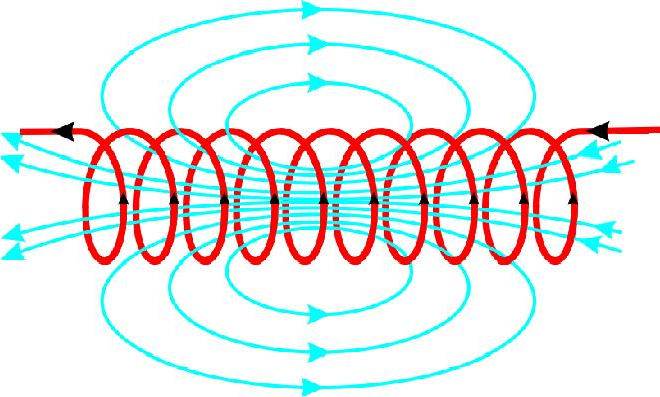
\includegraphics[height=2.5cm]{solenoid_field.png}};
  \node[anchor=south west,text width=8.2cm,font=\small,align=left] at ([xshift=1cm,yshift=0.35cm]current page.south west) {%
    \textbf{Complete classroom deck}: every derivation worked step by step with reasons, labelled diagrams, solved numericals, all textbook questions.\\[4pt]
    \textcolor{gray}{Figures: SCERT Class X Physical Science textbook, pp.\,219--248}};
\end{tikzpicture}
\end{frame}

% =====================================================================
\begin{frame}{Chapter roadmap}
\begin{columns}[T]
\column{0.5\textwidth}
\begin{tcolorbox}[colback=emblue!6,colframe=emblue,title={\textbf{Part A: Currents make magnetic fields}}]
\small
\begin{enumerate}
\item[10.1] Oersted experiment
\item[10.2] Magnetic field, field lines, flux $\Phi$, flux density $B$
\item[10.3] Field of a straight wire, circular coil, solenoid
\end{enumerate}
\end{tcolorbox}
\begin{tcolorbox}[colback=empurple!6,colframe=empurple,title={\textbf{Part B: Fields push on currents}}]
\small
\begin{enumerate}
\item[10.4] $F=qvB\sin\theta$, $F=ILB\sin\theta$, circular motion
\item[10.4] Electric motor
\end{enumerate}
\end{tcolorbox}
\column{0.5\textwidth}
\begin{tcolorbox}[colback=emgreen!6,colframe=emgreen,title={\textbf{Part C: Changing fields make currents}}]
\small
\begin{enumerate}
\item[10.5] Electromagnetic induction
\item[10.5] Faraday's law, Lenz's law
\item[10.5] Derivation: motional emf $\varepsilon=Blv$
\item[10.5] Applications, magnetic levitation
\item[10.5] AC and DC generators
\end{enumerate}
\end{tcolorbox}
\begin{examtip}[How to use this deck]
\small Badges \badge{1M} \badge{2M} \badge{4M} show usual marks. \textbf{Derivation} frames show \emph{step, working, reason}. Answers to \textbf{Teacher asks} appear on the next click.
\end{examtip}
\end{columns}
\end{frame}

% =====================================================================
\begin{frame}{Recall and warm-up}
\begin{columns}[c]
\column{0.52\textwidth}
\begin{itemize}
\item A magnet has two poles, N and S. Like poles repel, unlike poles attract.
\item A freely suspended magnet (compass needle) rests along the \textbf{north--south} direction.
\item A \textbf{field force} acts without contact (gravity, electric, magnetic).
\item Electric current = charges in motion: $I=\dfrac{Q}{t}$.
\item Electric power $P=\varepsilon I$; work $W=Fs$; power $P=Fv$.
\end{itemize}
\column{0.45\textwidth}
\begin{think}[Warm-up questions]
\small
\begin{itemize}
\item How do electric motors and calling bells work?
\item How does an electromagnet work?
\item Is there any relation between electricity and magnetism?
\item Can we produce electricity from magnetism?
\end{itemize}
\end{think}
\end{columns}
\end{frame}

% =====================================================================

\section{Basics first}

% =====================================================================
\begin{frame}{The big picture: one story in three steps}
\centering
\begin{tikzpicture}
\node[story=emblue] (a) at (-5.4,0) {\textbf{\faBolt\ Electric current}\\ moving charges};
\node[story=emteal] (b) at (0,0) {\textbf{\faMagnet\ Magnetic field}\\ appears around the current};
\node[story=emorange] (c) at (5.4,0) {\textbf{\faCog\ Motion}\\ the field pushes things};
\draw[-{Stealth},very thick,emblue] (a) -- node[above,font=\footnotesize,align=center]{\textbf{Part A}\\Oersted} (b);
\draw[-{Stealth},very thick,empurple] (b) -- node[above,font=\footnotesize,align=center]{\textbf{Part B}\\Motor} (c);
\draw[-{Stealth},very thick,emgreen,rounded corners=8pt] (c.south) -- ++(0,-1.3) -- node[below,font=\footnotesize]{\textbf{Part C}: moving a magnet makes current again (Generator)} ($(a.south)+(0,-1.3)$) -- (a.south);
\end{tikzpicture}
\vspace{6pt}
\begin{simple}[Remember this one line]
Electricity and magnetism are \textbf{two faces of the same thing}. Current makes magnetism; magnetism pushes current; changing magnetism makes current.
\end{simple}
\end{frame}
% =====================================================================
\begin{frame}{Basics 1: What is a magnet?}
\begin{columns}[c]
\column{0.5\textwidth}\centering
\begin{tikzpicture}[scale=0.85]
\foreach \y/\l/\r in {1.6/N/S,0.4/S/N,-0.8/N/N}{
 \ifx\l N \def\cl{emred}\else\def\cl{emblue}\fi
 \ifx\r N \def\cr{emred}\else\def\cr{emblue}\fi
 \fill[\cl] (-2.6,\y) rectangle (-1.3,\y+0.55); \node[white,font=\bfseries] at (-1.95,\y+0.27) {\l};
 \fill[\cr] (1.3,\y) rectangle (2.6,\y+0.55); \node[white,font=\bfseries] at (1.95,\y+0.27) {\r};}
\draw[-{Stealth},thick,emgreen] (-1.0,1.87) -- (-0.1,1.87); \draw[-{Stealth},thick,emgreen] (1.0,1.87) -- (0.1,1.87);
\node[font=\small\bfseries,emgreen!60!black] at (0,1.5) {attract};
\draw[-{Stealth},thick,emgreen] (-1.0,0.67) -- (-0.1,0.67); \draw[-{Stealth},thick,emgreen] (1.0,0.67) -- (0.1,0.67);
\node[font=\small\bfseries,emgreen!60!black] at (0,0.3) {attract};
\draw[-{Stealth},thick,emred] (-0.1,-0.53) -- (-1.0,-0.53); \draw[-{Stealth},thick,emred] (0.1,-0.53) -- (1.0,-0.53);
\node[font=\small\bfseries,emred] at (0,-0.9) {repel};
\end{tikzpicture}
\column{0.48\textwidth}
\begin{itemize}
\item Every magnet has \textbf{two poles}: North (N) and South (S).
\item \textbf{Unlike} poles attract. \textbf{Like} poles repel.
\item You can never get a single pole: cut a magnet and each piece has both N and S.
\item Magnets attract iron, nickel and cobalt.
\end{itemize}
\begin{simple}[Think of it like this]
A \textbf{compass needle} is a tiny magnet. Its N end always swings to the Earth's geographic north because the Earth itself acts like a giant magnet.
\end{simple}
\end{columns}
\end{frame}
% =====================================================================
\begin{frame}{Basics 2: What is a ``field''?}
\begin{columns}[c]
\column{0.5\textwidth}
\begin{simple}[Kitchen smell analogy]
Cooking in a kitchen: you smell it \textbf{without touching} the food.
\begin{itemize}
\item Strong smell near the stove; weak far away $\Rightarrow$ \textbf{strength} changes with place.
\item Smell drifts \emph{from} the stove \emph{towards} you $\Rightarrow$ it has a \textbf{direction}.
\end{itemize}
\end{simple}
\begin{defn}[Field]
\small Space around an object where it can push or pull other things \textbf{without touching}. A field has \key{strength} and \key{direction} at every point.
\end{defn}
\column{0.46\textwidth}\centering
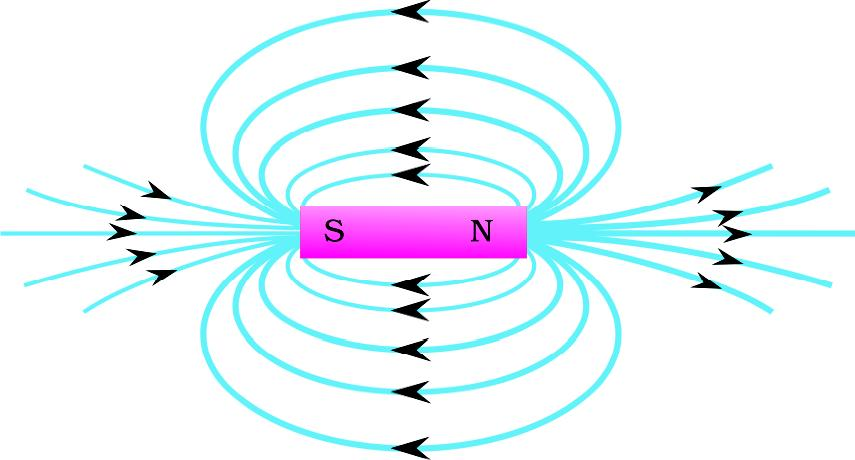
\includegraphics[width=0.95\linewidth]{bar_field.png}\\
{\scriptsize Magnetic field of a bar magnet. Each curve is a \textbf{field line}: the arrow shows the direction; crowded lines mean a stronger field.}
\end{columns}
\end{frame}
% =====================================================================
\begin{frame}{Basics 3: What is electric current?}
\begin{columns}[c]
\column{0.5\textwidth}\centering
\begin{tikzpicture}
\draw[very thick] (0,0) -- (1.7,0) (2.5,0) -- (4.4,0) -- (4.4,0.9) (4.4,1.5) -- (4.4,2.4) -- (0,2.4) -- (0,0);
\draw[very thick] (1.7,-0.4) -- (1.7,0.4); \draw[ultra thick] (2.5,-0.22) -- (2.5,0.22);
\node[font=\footnotesize] at (1.7,-0.75) {$+$}; \node[font=\footnotesize] at (2.5,-0.75) {$-$};
\node[font=\footnotesize] at (2.1,-1.2) {battery};
\fill[yellow!70,draw=black,thick] (4.4,1.2) circle (0.3); \node[font=\footnotesize,anchor=west] at (4.75,1.2) {bulb};
\draw[cur] (1.1,2.4) -- (3.3,2.4) node[midway,above=3pt,font=\footnotesize,emred]{current $I$ drawn $+\to-$};
\foreach \x in {0.5,1.3,2.1,2.9,3.7}\fill[emblue] (\x,0) circle (2.5pt);
\draw[-{Stealth},emblue,thick] (3.8,0.45) -- (0.6,0.45);
\node[font=\footnotesize,emblue] at (2.2,0.8) {electrons really go this way};
\end{tikzpicture}
\column{0.48\textwidth}
\begin{itemize}
\item Current is the \textbf{flow of charge}, like water flowing in a pipe.
\item Battery = pump, wire = pipe, charge = water.
\end{itemize}
\begin{formula}[Current]
\[I=\frac{Q}{t}\quad\text{unit: ampere (A)}\]
\small $1\,\text{A}=1$ coulomb of charge per second.
\end{formula}
\begin{simple}[Direction convention]
We \textbf{draw} current from $+$ to $-$ (old convention). Electrons really go the other way. Always follow the \textbf{drawn} direction in this chapter.
\end{simple}
\end{columns}
\end{frame}
% =====================================================================
\begin{frame}{Basics 4: Reading arrows into and out of the page}
\begin{columns}[c]
\column{0.5\textwidth}\centering
\begin{tikzpicture}
% dart side view
% toward you
\node[font=\footnotesize,align=center] at (0.2,0.2) {\textbf{towards you}\\you see the \textbf{tip}};
\draw[thick,fill=white] (2.4,0.2) circle (0.4); \fill (2.4,0.2) circle (0.1);
\node[font=\Large\bfseries,emred] at (3.5,0.2) {$\odot$};
% away
\node[font=\footnotesize,align=center] at (0.2,-1.5) {\textbf{away from you}\\you see the \textbf{tail feathers}};
\draw[thick,fill=white] (2.4,-1.5) circle (0.4); \draw[thick] (2.4-0.28,-1.5-0.28)--(2.4+0.28,-1.5+0.28) (2.4-0.28,-1.5+0.28)--(2.4+0.28,-1.5-0.28);
\node[font=\Large\bfseries,emblue] at (3.5,-1.5) {$\otimes$};
\end{tikzpicture}
\column{0.48\textwidth}
\begin{itemize}
\item $\odot$ (dot) $\Rightarrow$ pointing \textbf{out of the page}, towards you.
\item $\otimes$ (cross) $\Rightarrow$ pointing \textbf{into the page}, away from you.
\item A page full of $\times$ means a magnetic field going \textbf{into} the page; full of $\cdot$ means \textbf{out}.
\end{itemize}
\begin{simple}[Memory trick]
\textbf{D}ot = \textbf{D}ooming at you (the \emph{tip} is coming at you).\\ \textbf{C}ross = \textbf{C}arrying away (you see the \emph{tail}, it is leaving).
\end{simple}
\end{columns}
\end{frame}
% =====================================================================
\begin{frame}{Basics 5: Your right hand is the tool of this chapter}
\begin{columns}[T]
\column{0.33\textwidth}\centering
\textbf{\color{emblue}Rule 1: thumb rule}\\[2pt]
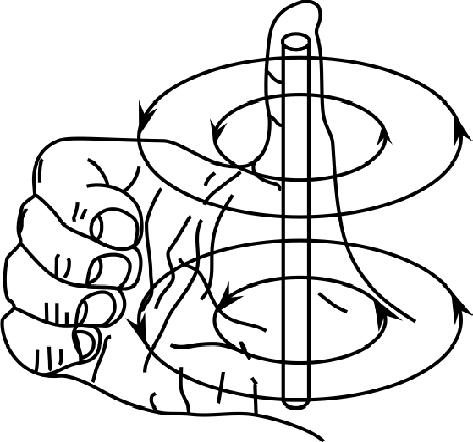
\includegraphics[height=2.4cm]{thumb_rule.png}\\
{\small Straight wire.\\ \textbf{Thumb} = current.\\ \textbf{Curled fingers} = field.}
\column{0.33\textwidth}\centering
\textbf{\color{emteal}Rule 2: coil rule}\\[2pt]
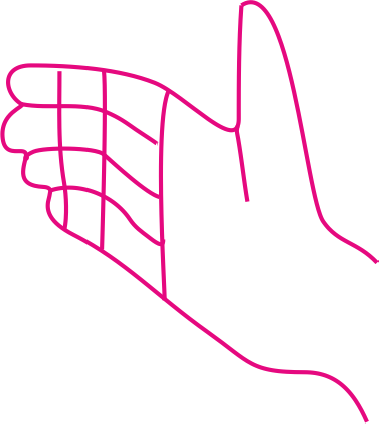
\includegraphics[height=2.4cm]{coil_hand.png}\\
{\small Coil or solenoid.\\ \textbf{Curled fingers} = current.\\ \textbf{Thumb} = N pole.}
\column{0.33\textwidth}\centering
\textbf{\color{emorange}Rule 3: force rule}\\[2pt]

\includegraphics[height=2.4cm]{rh_rule_b.png}\\
{\small Force on current/charge.\\ \textbf{Forefinger} = current $I$ (or $v$),\\ \textbf{middle finger} = field $B$,\\ \textbf{thumb} = force $F$.}
\end{columns}
\vspace{4pt}
\begin{simple}[Always ask: ``What do I know, and what do I want?'']
Know the \textbf{current}, want the \textbf{field}? Rule 1 or 2. Know the \textbf{current and field}, want the \textbf{push}? Rule 3. Use your \textbf{right} hand only.
\end{simple}
\end{frame}
% =====================================================================
\begin{frame}{Basics 6: Symbols and units you will meet}
\centering\renewcommand{\arraystretch}{1.25}
\begin{tabular}{@{}llll@{}}
\toprule
\textbf{Quantity} & \textbf{Symbol} & \textbf{SI unit} & \textbf{In plain words}\\
\midrule
Electric current & $I$ & ampere (A) & how fast charge flows\\
Charge & $q$ or $Q$ & coulomb (C) & amount of electric charge\\
Velocity & $v$ & m/s & speed with direction\\
Magnetic flux density & $B$ & tesla (T) & strength of the field\\
Magnetic flux & $\Phi$ & weber (Wb) & total field passing through an area\\
Force & $F$ & newton (N) & a push or pull\\
Induced emf & $\varepsilon$ & volt (V) & electrical ``push'' that drives current\\
\bottomrule
\end{tabular}
\vspace{4pt}
\begin{examtip}[Unit tip]
$1\,\text{T}=1\,\text{Wb/m}^2$. Convert first: cm $\to$ m, cm$^2\to$ m$^2$ (divide by $10^4$), before substituting into formulas.
\end{examtip}
\end{frame}
% =====================================================================
\begin{frame}{Maths 1: Powers of ten (scientific notation)}
\begin{columns}[T]
\column{0.5\textwidth}
\begin{simple}[Why?]
Physics numbers can be huge or tiny. Charge of a proton: $0.00000000000000000016$ C. Write it as $\mathbf{1.6\times10^{-19}}$ C.
\end{simple}
\begin{itemize}
\item $10^{3}=1000$,\; $10^{-3}=\dfrac{1}{1000}=0.001$
\item Move the point \textbf{left} $\Rightarrow$ power goes \textbf{up}; move \textbf{right} $\Rightarrow$ power goes \textbf{down}.
\end{itemize}
\column{0.48\textwidth}
\begin{formula}[Rules]
\[10^{a}\times10^{b}=10^{a+b}\qquad\frac{10^{a}}{10^{b}}=10^{a-b}\]
\end{formula}
\begin{answer}[Worked example]
$(2\times10^{6})\times(1.6\times10^{-19})\times0.5$\\
Numbers: $2\times1.6\times0.5=1.6$\\
Powers: $10^{6-19}=10^{-13}$\\
Answer: $\mathbf{1.6\times10^{-13}}$
\end{answer}
\end{columns}
\end{frame}
% =====================================================================
\begin{frame}{Maths 2: Changing units before you calculate}
\centering\renewcommand{\arraystretch}{1.25}
\begin{tabular}{@{}lll@{}}
\toprule
\textbf{Change} & \textbf{How} & \textbf{Example}\\
\midrule
cm $\to$ m & divide by 100 & $20\ \text{cm}=0.2$ m\\
mm $\to$ m & divide by 1000 & $5.7$ mm $=5.7\times10^{-3}$ m\\
cm$^2\to$ m$^2$ & divide by $10^{4}$ (not 100!) & $4\ \text{cm}^2=4\times10^{-4}$ m$^2$\\
minutes $\to$ s & multiply by 60 & $0.2$ min $=12$ s\\
\bottomrule
\end{tabular}
\vspace{6pt}
\begin{simple}[Why $10^4$ for area?]
$1\ \text{cm}=\frac{1}{100}$ m, so $1\ \text{cm}^2=\frac{1}{100}\times\frac{1}{100}=\frac{1}{10\,000}$ m$^2$. Area squares the conversion factor.
\end{simple}
\end{frame}
% =====================================================================
\begin{frame}{Maths 3: Rearranging a formula (the balance method)}
\begin{columns}[T]
\column{0.5\textwidth}
\begin{simple}[Golden rule]
An equation is a balance. Whatever you do to one side, do the \textbf{same} to the other.
\end{simple}
Start with $F=ILB$.
\begin{itemize}
\item Find $B$: divide both sides by $IL$ $\Rightarrow$ $B=\dfrac{F}{IL}$
\item Find $I$: divide both sides by $LB$ $\Rightarrow$ $I=\dfrac{F}{LB}$
\item Find $L$: divide both sides by $IB$ $\Rightarrow$ $L=\dfrac{F}{IB}$
\end{itemize}
\column{0.48\textwidth}
\begin{answer}[Example from the chapter]
$r=\dfrac{mv}{Bq}$. Find $v$.\\[3pt]
Multiply both sides by $Bq$: $rBq=mv$\\
Divide both sides by $m$: $v=\dfrac{rBq}{m}$
\end{answer}
\begin{examtip}[Steps for every numerical]
1. Write the formula. 2. Convert units. 3. Rearrange if needed. 4. Substitute. 5. Calculate and write the \textbf{unit}.
\end{examtip}
\end{columns}
\end{frame}
% =====================================================================
\begin{frame}{Maths 4: Sine and cosine of an angle}
\begin{columns}[c]
\column{0.42\textwidth}\centering
\begin{tikzpicture}[scale=0.95]
\draw[thick] (0,0) -- (2.6,0) -- (2.6,1.5) -- cycle;
\draw[thick] (2.45,0) -- (2.45,0.15) -- (2.6,0.15);
\draw (0.6,0) arc (0:30:0.6); \node[font=\small] at (0.85,0.17) {$\theta$};
\node[font=\small,emblue] at (1.3,-0.3) {adjacent};
\node[font=\small,emred,rotate=90] at (2.95,0.75) {opposite};
\node[font=\small,emteal,rotate=30] at (1.15,1.0) {hypotenuse};
\end{tikzpicture}
{\small$\sin\theta=\dfrac{\text{opposite}}{\text{hypotenuse}}$\\[4pt]$\cos\theta=\dfrac{\text{adjacent}}{\text{hypotenuse}}$}
\column{0.56\textwidth}
\small\centering\renewcommand{\arraystretch}{1.2}
\begin{tabular}{@{}c|ccccc@{}}
$\theta$ & $0^\circ$ & $30^\circ$ & $45^\circ$ & $60^\circ$ & $90^\circ$\\\hline
$\sin\theta$ & $0$ & $\tfrac12$ & $\tfrac{1}{\sqrt2}$ & $\tfrac{\sqrt3}{2}$ & $1$\\
$\cos\theta$ & $1$ & $\tfrac{\sqrt3}{2}$ & $\tfrac{1}{\sqrt2}$ & $\tfrac12$ & $0$\\
\end{tabular}
\vspace{4pt}
\begin{simple}[Where we use them]
$F=qvB\sin\theta$: $\theta$ is the angle between $v$ and $B$. At $90^\circ$ the force is maximum; at $0^\circ$ it is zero.\\
$\Phi=BA\cos\theta$: $\theta$ is the angle between $B$ and the \textbf{normal} to the plane. At $0^\circ$ the flux is maximum.
\end{simple}
\end{columns}
\end{frame}
% =====================================================================
\begin{frame}{Maths 5: Area, circles and time period}
\begin{columns}[T]
\column{0.5\textwidth}
\begin{formula}[Shapes]
\small Rectangle: $A=\text{length}\times\text{breadth}$\\
Circle: $A=\pi r^{2}$, circumference $=2\pi r$ ($\pi\approx3.14$)
\end{formula}
\begin{answer}[Example]
Loop of radius $0.1$ m: $A=3.14\times0.1^{2}=0.0314$ m$^{2}$.
\end{answer}
\column{0.48\textwidth}
\begin{formula}[Speed, distance, time]
\[v=\frac{\text{distance}}{\text{time}}\;\Rightarrow\;\text{time}=\frac{\text{distance}}{v}\]
\end{formula}
\begin{simple}[Time period $T$]
Time for one full circle: $T=\dfrac{2\pi r}{v}$. We use this in the circular-path derivation.
\end{simple}
\end{columns}
\end{frame}
% =====================================================================
\begin{frame}{Maths 6: ``Change'' and ``rate of change'' ($\Delta$)}
\begin{columns}[c]
\column{0.5\textwidth}
\begin{itemize}
\item $\Delta$ (delta) means \textbf{change} = final $-$ initial.
\item $\Delta\Phi=\Phi_{\text{final}}-\Phi_{\text{initial}}$,\quad $\Delta t=t_{\text{final}}-t_{\text{initial}}$
\item \textbf{Rate of change} = change $\div$ time taken, e.g.\ $\varepsilon=\dfrac{\Delta\Phi}{\Delta t}$.
\end{itemize}
\begin{answer}[Example]
Flux falls from $0.5$ Wb to $0.1$ Wb in $0.2$ s.\\
$\Delta\Phi=0.1-0.5=-0.4$ Wb\\
$|\varepsilon|=\dfrac{0.4}{0.2}=\mathbf{2}$ V
\end{answer}
\column{0.46\textwidth}\centering
\begin{tikzpicture}[scale=0.85]
\draw[-{Stealth}] (0,0) -- (4.2,0) node[right,font=\small]{$t$ (s)};
\draw[-{Stealth}] (0,0) -- (0,3) node[above,font=\small]{$\Phi$ (Wb)};
\draw[very thick,emblue] (0,2.5) -- (3.2,0.5);
\draw[dashed] (0,2.5) -- (3.2,2.5) -- (3.2,0.5);
\node[font=\small] at (1.6,2.8) {$\Delta t$}; \node[font=\small,anchor=west] at (3.25,1.5) {$\Delta\Phi$};
\end{tikzpicture}\\
{\small Slope of a flux--time graph = $\dfrac{\Delta\Phi}{\Delta t}$ = induced emf. A steeper line means a bigger emf; a flat line means zero emf.}
\end{columns}
\end{frame}
% =====================================================================
\begin{frame}{Maths 7: Proportion, ``if this doubles, what happens?''}
\begin{columns}[T]
\column{0.55\textwidth}
\renewcommand{\arraystretch}{1.3}\small
\begin{tabular}{@{}lll@{}}
\toprule
\textbf{Formula} & \textbf{If this doubles\ldots} & \textbf{That}\\
\midrule
$F=ILB$ & $B$ doubles & $F$ doubles\\
$F=ILB$ & $I$ and $L$ both double & $F$ becomes $4\times$\\
$r=\dfrac{mv}{Bq}$ & $B$ doubles & $r$ \textbf{halves}\\
$\varepsilon=Blv$ & $v$ doubles & $\varepsilon$ doubles\\
$\Phi=BA\cos\theta$ & $A$ doubles & $\Phi$ doubles\\
\bottomrule
\end{tabular}
\column{0.43\textwidth}
\begin{simple}[Two kinds of relation]
\textbf{Direct} ($F\propto B$): both grow together.\\
\textbf{Inverse} ($r\propto\frac{1}{B}$): one grows, the other shrinks.
\end{simple}
\begin{examtip}
Spot the variable on top (direct) or underneath (inverse) in the formula.
\end{examtip}
\end{columns}
\end{frame}
% =====================================================================
\begin{frame}{Maths check: try these}
\small
\begin{columns}[T]
\column{0.5\textwidth}
\begin{think}[Quick maths drill]
\begin{enumerate}
\item Write $0.0005$ in powers of ten.
\item Convert $50$ cm$^2$ to m$^2$.
\item $F=ILB$: find $L$ if $F=6$ N, $I=3$ A, $B=0.5$ T.
\item Value of $\sin30^\circ$ and $\cos60^\circ$?
\item Flux changes by $0.6$ Wb in $0.3$ s. Find $\varepsilon$.
\end{enumerate}
\end{think}
\column{0.46\textwidth}
\uncover<2->{\begin{answer}[Answers]
\begin{enumerate}
\item $5\times10^{-4}$
\item $5\times10^{-3}$ m$^2$
\item $L=\dfrac{6}{3\times0.5}=4$ m
\item both $\tfrac12$
\item $\varepsilon=\dfrac{0.6}{0.3}=2$ V
\end{enumerate}
\end{answer}}
\end{columns}
\end{frame}
% =====================================================================
\begin{frame}{Quick check before we start}
\small
\begin{columns}[T]
\column{0.5\textwidth}
\begin{think}[Try these (answers on the next click)]
\begin{enumerate}
\item Two N poles are brought close. Attract or repel?
\item Charge $6$ C flows in $2$ s. Find the current.
\item An arrow shows $\otimes$. Is it going into or out of the page?
\item Which hand do we use for the rules?
\end{enumerate}
\end{think}
\column{0.46\textwidth}
\uncover<2->{\begin{answer}[Answers]
\begin{enumerate}
\item Repel (like poles).
\item $I=Q/t=6/2=3$ A.
\item Into the page.
\item The right hand.
\end{enumerate}
\end{answer}}
\end{columns}
\end{frame}

\section{Part A: Magnetic field}
% =====================================================================
\begin{frame}{Part A: Currents make magnetic fields}
\begin{goals}
\large\begin{itemize}
\item Describe what Oersted observed and what it proves.
\item Draw and read \textbf{magnetic field lines}; tell a strong field from a weak one.
\item Explain \textbf{flux} $\Phi$ and \textbf{flux density} $B$, and use $\Phi=BA\cos\theta$.
\item Find the field direction around a wire, a coil and a solenoid with the \textbf{right hand rule}.
\end{itemize}
\end{goals}
\end{frame}

\begin{frame}{10.1 Oersted experiment (Activity 1) \hfill \badge{2M} \badge{4M}}
\begin{columns}[T]
\column{0.56\textwidth}
\centering
\figlab{oersted_setup.png}{width=\linewidth}{
\draw[fptr] (0.30,1.12) node[flab,anchor=south east]{copper wire (24 gauge)} -- (0.36,0.82);
\draw[fptr] (0.36,1.12) node[flab,anchor=south west]{wooden sticks} -- (0.50,0.95);
\draw[fptr] (0.36,1.12) -- (0.27,0.62);
\draw[fptr] (0.30,0.20) node[flab,anchor=north]{magnetic compass} -- (0.40,0.60);
\draw[fptr] (0.85,1.10) node[flab,anchor=south]{battery (3 V)} -- (0.66,0.78);
\draw[fptr] (0.72,0.10) node[flab,anchor=north]{key} -- (0.54,0.40);
\draw[fptr] (0.05,0.05) node[flab,anchor=north]{thermocol sheet} -- (0.15,0.40);}\\[12pt]
{\scriptsize fig-1: current-carrying wire above a compass}
\column{0.42\textwidth}
\small
\begin{enumerate}
\item Wire stretched through slits of two sticks, in series with battery and key. Compass below the wire.
\item Bring a bar magnet near: needle deflects (magnetic force).
\item Remove the magnet, switch \textbf{on}: needle \textbf{deflects again}!
\item Switch off: needle returns to N--S.
\end{enumerate}
\begin{answer}[Conclusion]
\small A \textbf{current-carrying wire produces a magnetic field} around it. Electricity and magnetism are related.
\end{answer}
\end{columns}
\end{frame}

% =====================================================================
\begin{frame}{Do you know? Hans Christian Oersted \hfill \badge{1M}}
\begin{columns}[c]
\column{0.26\textwidth}\centering
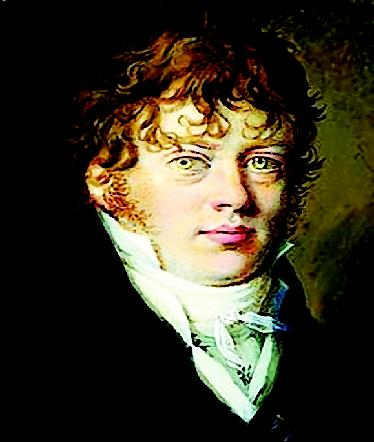
\includegraphics[width=0.9\linewidth]{oersted.png}\\{\scriptsize H.\,C.\ Oersted (1777--1851)}
\column{0.72\textwidth}
\begin{itemize}
\item In a lecture in April 1820 he placed a compass needle under a wire and switched on the current: the needle \textbf{deflected}.
\item Showed that electricity and magnetism are \textbf{interconnected}: the start of \key{electromagnetism}.
\item Led to the dynamo, the electric motor, radio, television and fibre optics.
\item The unit of magnetic field strength is named \imp{oersted} in his honour.
\end{itemize}
\end{columns}
\end{frame}

% =====================================================================
\begin{frame}{10.2 Magnetic field of a bar magnet (Activity 2) \hfill \badge{1M} \badge{2M}}
\begin{columns}[T]
\column{0.55\textwidth}
\begin{activity}[Activity 2: compass around a bar magnet]
\small Place a compass at many points around a bar magnet on paper. Mark the direction of the needle at each point (S $\to$ N of the needle).
\end{activity}
\small
\begin{itemize}
\item The needle points in \textbf{different directions} at different places $\Rightarrow$ the field has \textbf{direction} that varies from point to point.
\item Far from the magnet the needle points almost N--S $\Rightarrow$ \textbf{strength} decreases with distance.
\item Above the magnet the needle is also deflected $\Rightarrow$ the field is \textbf{three-dimensional}.
\end{itemize}
\column{0.43\textwidth}
\begin{defn}[Field]
\small A region where a force acts on an object \textbf{without physical contact}.
\end{defn}
\begin{defn}[Magnetic field]
\small The region surrounding a magnet in which its magnetic force can be felt. It is characterised by \key{strength} and \key{direction}.
\end{defn}
\end{columns}
\end{frame}

% =====================================================================
\begin{frame}{10.2.1 Magnetic field lines (Activity 3) \hfill \badge{1M} \badge{2M} \badge{Diagram}}
\begin{columns}[c]
\column{0.5\textwidth}\centering
\figlab{bar_field.png}{width=\linewidth}{
\draw[fptr] (0.12,1.08) node[flab,anchor=south]{field line} -- (0.30,0.93);
\draw[fptr] (0.88,1.08) node[flab,anchor=south]{lines crowded near poles (strong)} -- (0.72,0.62);
\draw[fptr] (0.50,-0.10) node[flab,anchor=north]{lines far apart (weak)} -- (0.50,0.04);}\\[12pt]
{\scriptsize fig-2: field lines of a bar magnet (outside: N $\to$ S)}
\column{0.48\textwidth}
\small
\textbf{Plotting:} put the compass at N, mark a dot at the tip of the needle, move the compass to the dot, repeat until you reach S. Join the dots.
\begin{itemize}
\item Field lines are \textbf{imaginary} curves.
\item \key{Tangent} at any point gives the direction of the field.
\item \textbf{Crowded} lines $\Rightarrow$ strong field; \textbf{spread} lines $\Rightarrow$ weak field.
\item \key{Non-uniform field}: strength \textbf{or} direction changes.\\ \key{Uniform field}: strength \textbf{and} direction constant (parallel, equally spaced lines).
\end{itemize}
\end{columns}
\end{frame}

% =====================================================================
\begin{frame}{10.2.2 Magnetic flux and flux density \hfill \badge{1M} \badge{2M}}
\begin{columns}[c]
\column{0.44\textwidth}\centering
\begin{tikzpicture}[scale=0.9]
\foreach \y in {-1.2,-0.6,0,0.6,1.2} \draw[fl=0.2] (-2.2,\y) -- (2.4,\y);
\fill[gray!35,opacity=0.8] (0,0) ellipse (0.28 and 1.05);
\draw[thick] (0,0) ellipse (0.28 and 1.05);
\node[flab] at (0.0,-1.6) {plane of area $A$};
\node[font=\small\bfseries,fieldc] at (-2.5,0.9) {$B$};
\node[font=\scriptsize,align=center] at (1.5,1.65) {plane $\perp$ field};
\end{tikzpicture}\\
{\scriptsize fig-3(a): lines crossing a plane placed perpendicular to a uniform field}
\column{0.54\textwidth}
\begin{defn}[Magnetic flux $\Phi$]
\small The number of field lines passing through a plane of area $A$ held \textbf{perpendicular} to the field. SI unit: \key{weber (Wb)}.
\end{defn}
\begin{defn}[Magnetic flux density $B$]
\small Flux passing through \textbf{unit area} held perpendicular to the field. Also called \key{magnetic induction}.
\[B=\frac{\Phi}{A}\qquad\text{unit: Wb/m}^2=\text{tesla (T)}\]
\end{defn}
\end{columns}
\end{frame}

% =====================================================================
\begin{frame}[shrink=8]{Flux in simple words: rain through a window}
\begin{columns}[c]
\column{0.6\textwidth}\centering
\begin{tikzpicture}[scale=0.6]
\foreach \ang/\xo/\lab in {90/0/{face-on: \textbf{most} lines},60/4.2/{tilted: \textbf{fewer}},0/8.4/{edge-on: \textbf{none}}}{
 \foreach \y in {-1.0,-0.5,0,0.5,1.0} \draw[fl=0.3] (\xo-1.2,\y) -- (\xo+1.2,\y);
 \draw[very thick,emorange] ($(\xo,0)+(\ang:1.3)$) -- ($(\xo,0)-(\ang:1.3)$);
 \node[font=\footnotesize,align=center] at (\xo,-1.8) {\lab};}
\end{tikzpicture}\\
{\scriptsize Orange line = the window seen edge-on; blue lines = field lines (rain).}
\column{0.38\textwidth}
\begin{simple}[Analogy]
Rain = field lines. Window = area $A$.
\begin{itemize}
\item Hold the window \textbf{face-on}: the most rain passes.
\item \textbf{Tilt} it: less passes.
\item \textbf{Edge-on}: no rain passes.
\end{itemize}
\textbf{Flux $\Phi$} = how much rain passes. \textbf{Flux density $B$} = how heavy the rain is.
\end{simple}
\end{columns}
\end{frame}

% =====================================================================
\begin{frame}[shrink=15]{Derivation 1: flux through a tilted plane, $\Phi=BA\cos\theta$ \hfill \badge{2M}}
\begin{columns}[T]
\column{0.4\textwidth}\centering
\begin{tikzpicture}[scale=0.95]
\foreach \y in {0.2,0.7,1.2,1.7,2.2} \draw[fl=0.15] (-0.5,\y) -- (3.8,\y);
\node[font=\small\bfseries,fieldc] at (-0.75,2.2) {$B$};
% tilted plane (edge view)
\draw[very thick,emorange] (1.2,0.1) -- (2.2,2.4);
\node[flab,anchor=west] at (2.25,2.5) {plane, area $A$};
% normal
\coordinate (C) at (1.7,1.25);
\draw[-{Stealth},thick,empurple] (C) -- ($(C)+(-23.5:1.3)$) node[below right,font=\scriptsize,empurple,fill=white,inner sep=1pt]{normal};
\draw[dashed,gray] (C) -- ($(C)+(1.3,0)$);
\draw[empurple] ($(C)+(0.6,0)$) arc (0:-23.5:0.6); \node[font=\scriptsize,empurple] at ($(C)+(-12:0.85)$) {$\theta$};
% projection perpendicular to field
\draw[thick,dashed,emgreen!70!black] (1.2,0.1) -- (1.2,2.4);
\node[font=\scriptsize,emgreen!60!black,align=center] at (0.55,-0.35) {effective area\\$A\cos\theta$ ($\perp$ field)};
\end{tikzpicture}\\
{\scriptsize fig-3(b): edge view of the plane}
\column{0.58\textwidth}
\begin{steps}[3.3cm]
\stp1 & B=\frac{\Phi}{A_{\perp}} & $B$ is always defined with the area \textbf{perpendicular} to the field\\
\stp2 & A_{\perp}=A\cos\theta & $\theta$ = angle between $B$ and the normal; only this part of the plane faces the field\\
\stp3 & B=\frac{\Phi}{A\cos\theta} & substitute step 2 in step 1\\
\stp4 & \Phi=BA\cos\theta & multiply both sides by $A\cos\theta$\\
\end{steps}
\begin{formula}[Special cases]
\small $\theta=0^\circ$ (plane $\perp$ field): $\Phi=BA$ (maximum)\\
$\theta=90^\circ$ (plane $\parallel$ field): $\Phi=BA\cos90^\circ=0$
\end{formula}
\end{columns}
\end{frame}

% =====================================================================
\begin{frame}{Solved numericals: flux and flux density \hfill \badge{2M}}
\small
\begin{columns}[T]
\column{0.5\textwidth}
\begin{tcolorbox}[colback=emblue!4,colframe=emblue,title={\textbf{Q1.} $B=0.5$ T through a loop of area $0.02$ m$^2$, loop $\perp$ field. Find $\Phi$.}]
\stp1 Plane $\perp$ field $\Rightarrow\theta=0^\circ$, $\cos0^\circ=1$.\\
\stp2 $\Phi=BA=0.5\times0.02=\boxed{0.01\ \text{Wb}}$
\end{tcolorbox}
\pause
\begin{tcolorbox}[colback=emblue!4,colframe=emblue,title={\textbf{Q2.} Same loop turned so the normal makes $60^\circ$ with $B$.}]
\stp1 $\Phi=BA\cos60^\circ=0.01\times\frac12=\boxed{0.005\ \text{Wb}}$
\end{tcolorbox}
\column{0.5\textwidth}
\pause
\begin{tcolorbox}[colback=emgreen!5,colframe=emgreen,title={\textbf{Q3.} Flux of $2\times10^{-3}$ Wb crosses $4$ cm$^2$ normally. Find $B$.}]
\stp1 $A=4\ \text{cm}^2=4\times10^{-4}$ m$^2$ \;(1 cm$^2=10^{-4}$ m$^2$)\\[2pt]
\stp2 $B=\dfrac{\Phi}{A}=\dfrac{2\times10^{-3}}{4\times10^{-4}}=\boxed{5\ \text{T}}$
\end{tcolorbox}
\pause
\begin{think}[Textbook question]
\small What is the flux through a plane held \textbf{parallel} to the field?\\
\onslide<5->{\textbf{Zero}: no field line crosses it ($\theta=90^\circ$).}
\end{think}
\end{columns}
\end{frame}

% =====================================================================
\begin{frame}{10.3.1 Field of a straight current-carrying wire (Activity 4) \hfill \badge{2M} \badge{4M}}
\begin{columns}[T]
\column{0.42\textwidth}\centering
\figlab{wire_setup.png}{height=0.6\textheight}{
\draw[fptr] (0.30,0.97) node[flab,anchor=south]{retort stand} -- (0.58,0.92);
\draw[fptr] (1.05,0.97) node[flab,anchor=south]{vertical wire} -- (0.84,0.75);
\draw[fptr] (1.02,0.02) node[flab,anchor=north]{compass needles} -- (0.85,0.51);
\draw[fptr] (0.62,0.02) node[flab,anchor=north]{plank} -- (0.70,0.50);
\draw[fptr] (-0.05,0.70) node[flab,anchor=east]{battery} -- (0.27,0.52);
\draw[fptr] (-0.05,0.45) node[flab,anchor=east]{switch} -- (0.38,0.49);
\draw[fptr] (-0.05,0.25) node[flab,anchor=east]{table} -- (0.10,0.35);}\\
{\scriptsize fig-4(a)}
\column{0.56\textwidth}
\small
\begin{enumerate}
\item Pass a vertical wire through a hole in a plank; place 6--10 compass needles on a circle around the hole.
\item Switch on (3 V battery).
\item The needles set along \textbf{tangents to the circle}.
\item Sprinkle iron filings: they form \textbf{concentric circles}.
\end{enumerate}
\begin{answer}[Conclusion]
\small Field lines of a straight wire are \textbf{concentric circles} centred on the wire, in a plane perpendicular to it. They are \imp{closed loops}. The field is stronger near the wire (circles closer).
\end{answer}
\end{columns}
\end{frame}

% =====================================================================
\begin{frame}[shrink=6]{Direction of the field: right hand thumb rule \hfill \badge{1M} \badge{2M}}
\begin{columns}[c]
\column{0.28\textwidth}\centering
\begin{tikzpicture}[scale=0.8]
\foreach \r/\p in {0.6/0.12,1.1/0.12,1.6/0.12} \draw[fl=\p] (0,0) circle (\r);
\foreach \r/\p in {0.6/0.62,1.1/0.62,1.6/0.62} \draw[fieldc,thick,postaction={decorate},decoration={markings,mark=at position \p with {\arrow{Stealth[length=5pt]}}}] (0,0) circle (\r);
\outpage{(0,0)}
\node[font=\scriptsize,align=center] at (0,-2.0) {current \textbf{out of} page\\field \textbf{anticlockwise}};
\end{tikzpicture}\\{\scriptsize fig-4(b)}
\column{0.28\textwidth}\centering
\begin{tikzpicture}[scale=0.8]
\foreach \r in {0.6,1.1,1.6} \draw[fieldc,thick,postaction={decorate},decoration={markings,mark=at position 0.12 with {\arrowreversed{Stealth[length=5pt]}},mark=at position 0.62 with {\arrowreversed{Stealth[length=5pt]}}}] (0,0) circle (\r);
\inpage{(0,0)}
\node[font=\scriptsize,align=center] at (0,-2.0) {current \textbf{into} page\\field \textbf{clockwise}};
\end{tikzpicture}\\{\scriptsize fig-4(c)}
\column{0.42\textwidth}\centering
\figlab{thumb_rule.png}{width=0.62\linewidth}{
\draw[cur] (0.63,0.80) -- (0.63,1.08) node[above,font=\scriptsize\bfseries,emred]{thumb: current $I$};
\draw[fptr] (1.10,0.55) node[flab,anchor=west,align=left]{fingers:\\field $B$} -- (0.97,0.72);}\\
{\scriptsize fig-4(d)}
\begin{defn}[Right hand thumb rule]
\small Grasp the wire with the right hand with the \textbf{thumb along the current}; the \textbf{curled fingers} give the direction of the field lines.
\end{defn}
\end{columns}
\vspace{2pt}
{\scriptsize Symbols: $\odot$ current/field out of the page (arrow tip);\quad $\otimes$ into the page (arrow tail).}
\end{frame}

% =====================================================================
\begin{frame}{10.3.2 Field of a circular coil (Activity 5) \hfill \badge{2M} \badge{4M}}
\begin{columns}[T]
\column{0.42\textwidth}\centering
\figlab{coil_setup.png}{width=0.95\linewidth}{
\draw[fptr] (0.10,1.08) node[flab,anchor=south]{circular coil (4--5 turns)} -- (0.34,0.90);
\draw[fptr] (0.62,1.08) node[flab,anchor=south]{compass at centre} -- (0.50,0.70);
\draw[fptr] (0.72,-0.06) node[flab,anchor=north]{to current supply} -- (0.88,0.58);
\draw[fptr] (0.72,-0.06) -- (0.64,0.30);}\\[8pt]
{\scriptsize fig-5(a)}
\column{0.56\textwidth}
\small
\begin{itemize}
\item Plot field lines with a compass around the coil.
\item At the centre the needle points \textbf{perpendicular to the plane of the coil}: the field there is along the axis.
\item Bring a compass near one face: its S pole points to the face $\Rightarrow$ that face acts as a \textbf{N pole}.
\end{itemize}
\begin{defn}[Right hand rule for a coil]
\small Curl the right-hand fingers along the \textbf{current}; the \textbf{thumb} gives the direction of the \textbf{field} (points out of the N face).
\end{defn}
\end{columns}
\end{frame}

\begin{frame}{Coil: which face is North? \hfill \badge{1M} \badge{2M}}
\begin{columns}[c]
\column{0.3\textwidth}\centering
\begin{tikzpicture}
\draw[emred,very thick,postaction={decorate},decoration={markings,mark=at position 0.25 with {\arrow{Stealth[length=6pt]}},mark=at position 0.75 with {\arrow{Stealth[length=6pt]}}}] (0,0) circle (1);
\node[font=\small\bfseries] at (0,0) {N};
\node[font=\scriptsize,align=center] at (0,-1.5) {anticlockwise current\\(as you see it)};
\node[font=\scriptsize,align=center,fieldc] at (0,1.45) {$B$ towards you $\odot$};
\end{tikzpicture}
\column{0.3\textwidth}\centering
\begin{tikzpicture}
\draw[emred,very thick,postaction={decorate},decoration={markings,mark=at position 0.25 with {\arrowreversed{Stealth[length=6pt]}},mark=at position 0.75 with {\arrowreversed{Stealth[length=6pt]}}}] (0,0) circle (1);
\node[font=\small\bfseries] at (0,0) {S};
\node[font=\scriptsize,align=center] at (0,-1.5) {clockwise current\\(as you see it)};
\node[font=\scriptsize,align=center,fieldc] at (0,1.45) {$B$ away from you $\otimes$};
\end{tikzpicture}
\column{0.38\textwidth}\centering
\figlab{coil_hand.png}{width=0.52\linewidth}{
\draw[fptr] (1.08,0.95) node[flab,anchor=west]{thumb: $B$} -- (0.70,0.97);
\draw[fptr] (-0.08,0.45) node[flab,anchor=east,align=right]{fingers:\\current $I$} -- (0.12,0.70);}\\
{\scriptsize fig-5(b): right hand rule for a coil}
\begin{examtip}
\small Memory aid: letters \textbf{N} and \textbf{S} drawn with arrows at their ends run anticlockwise and clockwise respectively.
\end{examtip}
\end{columns}
\end{frame}

% =====================================================================
\begin{frame}{10.3.3 Field of a solenoid (Activity 6) \hfill \badge{2M} \badge{4M}}
\begin{columns}[T]
\column{0.4\textwidth}\centering
\figlab{solenoid_setup.png}{height=0.26\textheight}{
\draw[fptr] (0.12,1.08) node[flab,anchor=south]{solenoid (long helix)} -- (0.36,0.84);
\draw[fptr] (0.70,-0.05) node[flab,anchor=north]{to current supply} -- (0.83,0.52);}\\[4pt]
{\scriptsize fig-6(a)}\\[8pt]
\figlab{solenoid_field.png}{height=0.27\textheight}{
\node[font=\small\bfseries,emred] at (-0.04,0.5) {N};
\node[font=\small\bfseries,emred] at (1.04,0.5) {S};
\node[font=\scriptsize\bfseries,emred] at (0.08,0.80) {$I$};
\node[font=\scriptsize\bfseries,emred] at (0.93,0.80) {$I$};
}\\[2pt]
{\scriptsize fig-6(b): field lines (iron filings)}
\column{0.58\textwidth}
\small
\begin{defn}[Solenoid]
\small A long wire wound in a \textbf{close-packed helix}.
\end{defn}
\begin{itemize}
\item Iron filings show a pattern like that of a \textbf{bar magnet}: a solenoid behaves like a bar magnet.
\item One end is N, the other S (find with the right hand rule).
\item Outside: field lines go \textbf{N $\to$ S}; inside: \textbf{S $\to$ N}, strong and nearly uniform (parallel lines).
\item Lines outside are continuous with those inside $\Rightarrow$ field lines are \imp{closed loops}. Same for a bar magnet.
\end{itemize}
\begin{answer}[Big idea]
\small Moving charges (currents) produce magnetic fields.
\end{answer}
\end{columns}
\end{frame}

% =====================================================================
\section{Part B: Magnetic force}
% =====================================================================
\begin{frame}{Part B: Fields push on currents}
\begin{goals}
\large\begin{itemize}
\item Find the \textbf{direction and size} of the force on a moving charge, $F=qvB\sin\theta$.
\item Show why a charge in a field moves in a \textbf{circle}: $r=mv/Bq$.
\item Derive $F=ILB\sin\theta$ for a current-carrying wire.
\item Explain how an \textbf{electric motor} keeps turning.
\end{itemize}
\end{goals}
\end{frame}

\begin{frame}{10.4 Force on a moving charge (Activity 7) \hfill \badge{1M} \badge{2M}}
\begin{columns}[T]
\column{0.52\textwidth}
\begin{activity}[Activity 7: magnet near an old CRT TV]
\small The picture gets \textbf{distorted}; move the magnet away and it clears.
\end{activity}
\small The picture is made by a beam of \textbf{moving electrons}. The magnetic field exerts a force on them and changes their path: the \key{magnetic force}.
\begin{formula}[Magnetic force on a charge]
\[F=qvB\quad(\vec v\perp\vec B)\qquad F=qvB\sin\theta\]
$\theta$ = angle between $\vec v$ and $\vec B$.
\end{formula}
\column{0.46\textwidth}\centering
\begin{tikzpicture}[scale=0.95]
\foreach \x in {0,...,6}{\foreach \y in {0,...,4}{\node[font=\scriptsize,gray] at (\x*0.6,\y*0.6) {$\times$};}}
\fill[white] (0.9,0.95) rectangle (2.7,2.2);
\fill[emred] (1.2,1.2) circle (3pt) node[below left,font=\small]{$+q$};
\draw[vvec] (1.2,1.2) -- (2.5,1.2) node[below,font=\small]{$v$};
\draw[fvec] (1.2,1.2) -- (1.2,2.15) node[right,font=\small]{$F$};
\node[font=\small,fieldc] at (1.8,-0.45) {$B$ into the page ($\times$)};
\end{tikzpicture}\\
{\scriptsize fig-7: charge moving $\perp$ to $B$}
\begin{tcolorbox}[colback=emblue!4,colframe=emblue,title={\textbf{Special cases of $F=qvB\sin\theta$}}]
\small $\theta=90^\circ$: $F=qvB$ (maximum)\\
$\theta=0^\circ$ or $180^\circ$ (moving along or against $B$): $\sin\theta=0\Rightarrow$ \imp{$F=0$}\\
$v=0$ (charge at rest): $F=0$
\end{tcolorbox}
\end{columns}
\end{frame}

% =====================================================================
\begin{frame}[shrink=6]{Direction of the magnetic force: right hand rules \hfill \badge{1M} \badge{2M}}
\begin{columns}[T]
\column{0.48\textwidth}\centering
\figlab{rh_rule_a.png}{height=0.42\textheight}{
\node[font=\small\bfseries,emgreen!60!black,anchor=south] at (0.21,1.0) {$F$ (thumb)};
\node[font=\small\bfseries,fieldc,anchor=west] at (0.90,0.47) {$B$};
\node[font=\small\bfseries,empurple,anchor=west] at (0.84,0.06) {$v$};}\\
{\scriptsize fig-8(a): fingers along $v$, curl towards $B$; thumb gives $F$}
\column{0.5\textwidth}\centering
\figlab{rh_rule_b.png}{height=0.42\textheight}{
\node[font=\small\bfseries,emgreen!60!black,anchor=south] at (0.83,1.0) {$F$ (thumb)};
\node[font=\small\bfseries,empurple,anchor=south] at (0.12,0.55) {forefinger: $v$ or $I$};
\node[font=\scriptsize\bfseries,fieldc,anchor=north,align=center] at (0.55,0.0) {middle finger: $B$ (out of paper)};}\\[8pt]
{\scriptsize fig-8(b): three fingers mutually perpendicular}
\end{columns}
\vspace{2pt}
\begin{examtip}
\small $F$ is always \textbf{perpendicular to both} $v$ and $B$. Rules are for a \textbf{positive} charge; for a \textbf{negative} charge (electron) find the direction for $+q$, then \textbf{reverse} it.
\end{examtip}
\end{frame}

% =====================================================================
\begin{frame}[shrink=6]{Derivation 2: circular path of a charge, $r=\dfrac{mv}{Bq}$, $T=\dfrac{2\pi m}{Bq}$ \hfill \badge{4M}}
\begin{columns}[T]
\column{0.36\textwidth}\centering
\begin{tikzpicture}[scale=0.72]
\xgrid{-4}{4}{-4}{4}
\draw[fieldc!60,dashed,thick] (0,0) circle (1.5);
\foreach \a in {0,90,180,270}{
  \coordinate (P) at (\a:1.5);
  \fill[emred] (P) circle (2.5pt);
  \draw[vvec] (P) -- ($(P)+(\a+90:0.8)$);
  \draw[fvec] (P) -- ($(P)+(\a+180:0.7)$);}
\node[font=\scriptsize,empurple] at (1.95,0.6) {$v$};
\node[font=\scriptsize,emgreen!60!black] at (1.05,0.2) {$F$};
\draw[gray] (0,0) -- (-1.06,-1.06) node[midway,left,font=\scriptsize]{$r$};
\fill (0,0) circle (1.2pt);
\end{tikzpicture}\\
{\scriptsize fig-E-1: $F\perp v$ always, towards the centre}
\column{0.62\textwidth}
\begin{steps}[3.6cm]
\stp1 & F=qvB & $v\perp B$, so $\sin90^\circ=1$\\
\stp2 & F\perp v & force never changes the speed, only the direction $\Rightarrow$ uniform circular motion\\
\stp3 & \frac{mv^2}{r}=qvB & magnetic force supplies the centripetal force\\
\stp4 & r=\frac{mv}{Bq} & multiply by $r$, cancel one $v$, divide by $qB$\\
\stp5 & T=\frac{2\pi r}{v} & time = circumference $\div$ speed\\
\stp6 & T=\frac{2\pi}{v}\cdot\frac{mv}{Bq}=\frac{2\pi m}{Bq} & substitute $r$; $v$ cancels\\
\end{steps}
\end{columns}
{\small\textbf{Note:} $T$ does \textbf{not} depend on speed: a faster particle moves in a bigger circle in the same time.}
\end{frame}

% =====================================================================
\begin{frame}{Solved numericals: force on a moving charge \hfill \badge{2M}}
\small
\begin{columns}[T]
\column{0.5\textwidth}
\begin{tcolorbox}[colback=emblue!4,colframe=emblue,title={\textbf{Q1.} A proton ($1.6\times10^{-19}$ C) moves at $2\times10^6$ m/s $\perp$ to $B=0.5$ T. Find $F$.}]
\stp1 $F=qvB$ \;($\theta=90^\circ$)\\
\stp2 $F=1.6\times10^{-19}\times2\times10^6\times0.5$\\
\stp3 $F=\boxed{1.6\times10^{-13}\ \text{N}}$
\end{tcolorbox}
\pause
\begin{tcolorbox}[colback=emblue!4,colframe=emblue,title={\textbf{Q2.} Same proton moves at $30^\circ$ to $B$.}]
\stp1 $F=qvB\sin30^\circ=1.6\times10^{-13}\times\frac12$\\
\stp2 $F=\boxed{8\times10^{-14}\ \text{N}}$
\end{tcolorbox}
\column{0.5\textwidth}
\pause
\begin{tcolorbox}[colback=emgreen!5,colframe=emgreen,title={\textbf{Q3.} Electron ($m=9.1\times10^{-31}$ kg) at $10^6$ m/s $\perp$ to $B=10^{-3}$ T. Radius?}]
\stp1 $r=\dfrac{mv}{Bq}=\dfrac{9.1\times10^{-31}\times10^6}{10^{-3}\times1.6\times10^{-19}}$\\[3pt]
\stp2 $=\dfrac{9.1\times10^{-25}}{1.6\times10^{-22}}=\boxed{5.7\times10^{-3}\ \text{m}}\approx5.7$ mm
\end{tcolorbox}
\pause
\begin{think}
\small A charge moves parallel to $B$. Force?\\
\onslide<5->{\textbf{Zero}, since $\sin0^\circ=0$.}
\end{think}
\end{columns}
\end{frame}

% =====================================================================
\begin{frame}[shrink=6]{Derivation 3: force on a current-carrying wire, $F=ILB$ \hfill \badge{4M}}
\begin{columns}[T]
\column{0.34\textwidth}\centering
\begin{tikzpicture}[scale=0.7]
\fill[fieldc!8] (-1.25,-1.5) rectangle (1.25,1.5);
\xgrid{-2}{2}{-2}{2}
\draw[line width=2.5pt] (0,-2.4) -- (0,2.4);
\draw[cur] (0.3,-0.4) -- (0.3,0.8) node[right,font=\small]{$I$};
\draw[fvec] (-0.1,0) -- (-1.4,0) node[left,font=\small]{$F$};
\draw[{Stealth}-{Stealth},gray] (1.55,-1.5) -- (1.55,1.5) node[midway,right,font=\small,black]{$L$};
\node[font=\small,fieldc] at (-0.9,1.9) {$B\ (\times)$};
\end{tikzpicture}\\
{\scriptsize fig-9: only length $L$ lies in the field}\\[4pt]
\begin{examtip}
\scriptsize $\parallel B$: $F=0$.\; $\perp B$: $F=ILB$ (max). In fig-9 the force on the upward current is to the \textbf{left} (right hand rule).
\end{examtip}
\column{0.64\textwidth}
\begin{steps}[3.0cm]
\stp1 & F_0=qvB & force on one charge moving with drift velocity $v$ $\perp B$\\
\stp2 & F=QvB\;\cdots(1) & add up for the total charge $Q$ inside the field\\
\stp3 & t=\frac{L}{v}\Rightarrow v=\frac{L}{t}\;\cdots(2) & time for the charge to cross the length $L$\\
\stp4 & F=\frac{QLB}{t}=\frac{Q}{t}LB\;\cdots(3) & put (2) in (1)\\
\stp5 & I=\frac{Q}{t} & definition of current\\
\stp6 & F=ILB\;\cdots(4) & put step 5 in (3)\\
\stp7 & F=ILB\sin\theta\;\cdots(5) & $\theta$ = angle between current and field\\
\end{steps}
\end{columns}
\end{frame}

% =====================================================================
\begin{frame}{Activity 8: wire in a horseshoe magnet \hfill \badge{4M: experiment}}
\begin{columns}[T]
\column{0.5\textwidth}\centering
\figlab{wire_force_setup.png}{width=0.8\linewidth}{
\draw[fptr] (0.60,1.10) node[flab,anchor=south]{horseshoe magnet} -- (0.50,0.93);
\draw[fptr] (0.10,1.10) node[flab,anchor=south]{copper wire} -- (0.30,0.86);
\draw[fptr] (0.36,0.62) node[flab,anchor=east]{force $F$} -- (0.48,0.62);
\draw[fptr] (0.05,0.42) node[flab,anchor=east]{wooden stick} -- (0.23,0.45);
\draw[fptr] (0.35,0.05) node[flab,anchor=north]{9 V battery} -- (0.44,0.38);
\draw[fptr] (0.66,0.05) node[flab,anchor=north]{switch} -- (0.52,0.36);
\draw[fptr] (0.85,-0.12) node[flab,anchor=north]{wooden plank} -- (0.88,0.22);}\\[14pt]
{\scriptsize fig-10}
\column{0.46\textwidth}
\small
\begin{enumerate}
\item Stretch a copper wire between two split sticks; connect to a 9 V battery and switch.
\item Switch on and bring a horseshoe magnet around the wire.
\item The wire is \textbf{deflected}; the direction agrees with the right hand rule.
\item Reverse the magnet's poles, or reverse the current: the deflection \textbf{reverses}.
\end{enumerate}
\begin{answer}[Conclusion]
\small A current-carrying wire in a magnetic field experiences a force; its direction depends on the directions of the current and of the field.
\end{answer}
\end{columns}
\end{frame}

% =====================================================================
\begin{frame}{Why does the wire move? Combining the fields \hfill \badge{2M} \badge{4M}}
\begin{columns}[c]
\column{0.24\textwidth}\centering
\begin{tikzpicture}[scale=0.7]
\foreach \y in {-1.2,-0.6,0,0.6,1.2} \draw[fl=0.55] (-1.4,\y) -- (1.4,\y);
\node[font=\small\bfseries] at (-1.7,0) {N}; \node[font=\small\bfseries] at (1.7,0) {S};
\end{tikzpicture}\\{\scriptsize (a) magnet's field}
\column{0.24\textwidth}\centering
\begin{tikzpicture}[scale=0.7]
\foreach \r in {0.45,0.9,1.35} \draw[fieldc,thick,postaction={decorate},decoration={markings,mark=at position 0.25 with {\arrowreversed{Stealth[length=4pt]}},mark=at position 0.75 with {\arrowreversed{Stealth[length=4pt]}}}] (0,0) circle (\r);
\inpage{(0,0)}
\end{tikzpicture}\\{\scriptsize (b) wire, current into page (clockwise)}
\column{0.24\textwidth}\centering
\figlab{combined_field.png}{width=0.85\linewidth}{
\node[flab,anchor=south] at (0.5,1.0) {strong (fields add)};
\node[flab,anchor=north] at (0.5,0.0) {weak (fields oppose)};
\draw[fvec] (0.5,0.46) -- (0.5,0.20);}\\[8pt]{\scriptsize (c) resultant: wire pushed to weak side}
\column{0.26\textwidth}
\small
\begin{itemize}
\item Above the wire, its clockwise field points \textbf{with} the magnet's field: strong.
\item Below, it points \textbf{against}: weak.
\item The non-uniform field pushes the wire from the strong to the \textbf{weak} region.
\end{itemize}
\end{columns}
\vspace{2pt}
{\scriptsize Check with the rule: $I$ into page, $B$ left to right $\Rightarrow F$ downward. \;fig-11(a),(b),(c)}
\end{frame}

% =====================================================================
\begin{frame}{Solved numericals: force on a wire \hfill \badge{2M}}
\small
\begin{columns}[T]
\column{0.5\textwidth}
\begin{tcolorbox}[colback=emblue!4,colframe=emblue,title={\textbf{Textbook App.\ Q4.} $F=8$ N on a 20 cm conductor $\perp$ to $B$, $I=40$ A. Find $B$.}]
\stp1 $L=20$ cm $=0.2$ m\\
\stp2 $F=ILB\Rightarrow B=\dfrac{F}{IL}$\\[2pt]
\stp3 $B=\dfrac{8}{40\times0.2}=\dfrac{8}{8}=\boxed{1\ \text{T}}$
\end{tcolorbox}
\pause
\begin{tcolorbox}[colback=emblue!4,colframe=emblue,title={\textbf{Q2.} $I=5$ A, $L=0.5$ m, $B=0.2$ T, wire at $30^\circ$ to $B$.}]
\stp1 $F=ILB\sin30^\circ=5\times0.5\times0.2\times\frac12=\boxed{0.25\ \text{N}}$
\end{tcolorbox}
\column{0.5\textwidth}
\pause
\begin{tcolorbox}[colback=emgreen!5,colframe=emgreen,title={\textbf{Textbook App.\ Q3 (fig-Q5).} Wire along its length, current $i$ upward, $B$ into page, length $L$ in field.}]
\begin{minipage}{0.3\linewidth}\centering
\begin{tikzpicture}[scale=0.55]
\xgrid{-2}{2}{-1}{1}
\draw[line width=2pt] (0,-1.2) -- (0,1.6);
\draw[cur] (0.3,0.3) -- (0.3,1.4) node[right,font=\scriptsize]{$i$};
\end{tikzpicture}
\end{minipage}\hfill
\begin{minipage}{0.66\linewidth}
\stp1 $\theta=90^\circ\Rightarrow F=iLB$\\
\stp2 Right hand rule: forefinger up ($i$), middle finger into page ($B$) $\Rightarrow$ thumb points \textbf{to the left}.
\end{minipage}
\end{tcolorbox}
\pause
\begin{think}
\small Force on a wire kept \textbf{parallel} to $B$?\\
\onslide<5->{\textbf{Zero}: every charge moves along the field.}
\end{think}
\end{columns}
\end{frame}

% =====================================================================
\begin{frame}{Motor in simple words}
\begin{simple}[Three ideas, in order]
\begin{enumerate}
\item A wire carrying current inside a magnetic field gets \textbf{pushed} sideways.
\item A coil has two long sides with currents in \textbf{opposite} directions, so one side is pushed \textbf{up} and the other \textbf{down}: the coil \textbf{spins}.
\item After half a turn the pushes would stop the spin. The \textbf{split ring (commutator)} reverses the current at that moment, so the coil keeps turning the same way.
\end{enumerate}
\end{simple}
\begin{examtip}[Pedal analogy]
Cycling: push down with one foot, then the other. The commutator is you switching feet at exactly the right time.
\end{examtip}
\end{frame}

% =====================================================================
\begin{frame}[shrink=6]{10.4.1 Electric motor: forces on a coil \hfill \badge{4M}}
\begin{columns}[c]
\column{0.44\textwidth}\centering
\begin{tikzpicture}[scale=0.9]
\foreach \y in {-1.6,-0.8,0,0.8,1.6} \draw[fl=0.08] (-2.6,\y) -- (2.6,\y);
\node[font=\small\bfseries,fieldc] at (2.6,2.0) {$B$};
\coordinate (A) at (-1,-1.2); \coordinate (Bc) at (-1,1.2); \coordinate (C) at (1,1.2); \coordinate (D) at (1,-1.2);
\draw[emred,line width=2pt] (A) -- (Bc) -- (C) -- (D) -- cycle;
\draw[cur] (-1.25,-0.5) -- (-1.25,0.5); \draw[cur] (1.25,0.5) -- (1.25,-0.5);
\node[below left,font=\small\bfseries] at (A) {A}; \node[above left,font=\small\bfseries] at (Bc) {B};
\node[above right,font=\small\bfseries] at (C) {C}; \node[below right,font=\small\bfseries] at (D) {D};
\inpage[0.16]{(-1.9,0.3)} \node[font=\scriptsize,emgreen!60!black] at (-1.9,-0.2) {$F$};
\outpage[0.16]{(1.9,0.3)} \node[font=\scriptsize,emgreen!60!black] at (1.9,-0.2) {$F$};
\end{tikzpicture}\\
{\scriptsize fig-12(a): current A$\to$B$\to$C$\to$D; $F$ on AB into page, on CD out of page}
\column{0.54\textwidth}
\small
\begin{enumerate}
\item AB and CD are always \textbf{perpendicular} to $B$ $\Rightarrow$ force $ILB$ on each.
\item Right hand rule: on AB (current up) force \textbf{into} the page; on CD (current down) force \textbf{out of} the page.
\item BC and DA: force zero when parallel to $B$; otherwise equal and opposite (up on BC, down on DA).
\item Forces on AB and CD: equal, opposite (equal currents in opposite directions) $\Rightarrow$ \imp{net force = 0}.
\item But they act along \textbf{different lines} $\Rightarrow$ they form a \key{couple} and \textbf{rotate} the coil, like two hands opening a bottle cap.
\end{enumerate}
\end{columns}
\end{frame}

% =====================================================================
\begin{frame}[shrink=6]{Electric motor: continuous rotation \hfill \badge{4M} \badge{Diagram}}
\begin{columns}[T]
\column{0.44\textwidth}\centering
\figlab{motor.png}{height=0.6\textheight}{
\node[font=\small\bfseries,emred] at (0.18,0.94) {N};
\node[font=\small\bfseries,emred] at (0.86,0.95) {S};
\draw[fptr] (0.55,1.05) node[flab,anchor=south]{coil ABCD, rotation axis} -- (0.58,0.84);
\draw[fptr] (-0.12,0.52) node[flab,anchor=east,align=right]{split rings\\C$_1$, C$_2$} -- (0.30,0.38);
\draw[fptr] (-0.12,0.52) -- (0.46,0.40);
\draw[fptr] (-0.12,0.30) node[flab,anchor=east,align=right]{brushes\\B$_1$, B$_2$} -- (0.12,0.37);
\draw[fptr] (-0.12,0.30) -- (0.58,0.30);
\node[font=\scriptsize\bfseries] at (0.13,0.00) {$+$};
\node[font=\scriptsize\bfseries] at (0.40,-0.02) {$-$};
\node[flab,anchor=north] at (0.27,-0.05) {battery};}\\[10pt]
{\scriptsize fig-12(c): simple electric motor}
\column{0.54\textwidth}
\footnotesize
\begin{itemize}
\item Without reversal: the coil turns to the vertical, overshoots by inertia, then the forces turn it \textbf{back}; it rocks to and fro.
\item \textbf{Fix:} reverse the current in the coil \textbf{every half rotation}.
\item The coil ends go to rings C$_1$, C$_2$ that rotate with it; fixed brushes B$_1$, B$_2$ connect to the battery.
\item After each half turn the rings swap brushes $\Rightarrow$ current in the coil reverses $\Rightarrow$ rotation continues in the \textbf{same direction}.
\end{itemize}
\begin{answer}[Energy]
\small Motor: \imp{electrical energy $\to$ mechanical energy}.
\end{answer}
\begin{tcolorbox}[colback=emteal!6,colframe=emteal,title={\textbf{Do you know? Fleming's left hand rule}}]
\scriptsize Stretch left-hand thumb, forefinger and middle finger mutually perpendicular: \textbf{forefinger} = field, \textbf{middle finger} = current, \textbf{thumb} = force (motion).
\end{tcolorbox}
\end{columns}
\end{frame}

% =====================================================================
\section{Part C: Electromagnetic induction}
% =====================================================================
\begin{frame}{Part C: Changing fields make currents}
\begin{goals}
\large\begin{itemize}
\item Explain \textbf{electromagnetic induction} with the magnet-and-coil activity.
\item State \textbf{Faraday's law} and \textbf{Lenz's law} and apply them.
\item Derive the motional emf $\varepsilon=Blv$.
\item Explain how \textbf{AC and DC generators} and magnetic levitation work.
\end{itemize}
\end{goals}
\end{frame}

\begin{frame}[shrink=6]{10.5 Electromagnetic induction (Activity 9) \hfill \badge{2M} \badge{4M}}
\begin{columns}[T]
\column{0.44\textwidth}\centering
\figlab{induction_setup.png}{width=0.82\linewidth}{
\node[font=\small\bfseries,emred] at (0.50,0.67) {N};
\draw[fptr] (0.62,1.08) node[flab,anchor=south]{bar magnet pushed in} -- (0.78,0.92);
\draw[fptr] (0.10,1.00) node[flab,anchor=south]{coil} -- (0.27,0.80);
\draw[fptr] (0.30,-0.08) node[flab,anchor=north]{galvanometer G} -- (0.11,0.07);}\\[12pt]
{\scriptsize fig-13}
\column{0.54\textwidth}
\footnotesize
\renewcommand{\arraystretch}{1.0}
\begin{tabular}{@{}p{3.3cm}p{2.6cm}@{}}
\toprule
\textbf{What we do} & \textbf{Galvanometer}\\
\midrule
Magnet at rest near coil & no deflection\\
N pole moved \textbf{towards} coil & deflects one way\\
N pole moved \textbf{away} & deflects the \textbf{other} way\\
S pole used instead & deflections reversed\\
Coil moved, magnet fixed & also deflects\\
\bottomrule
\end{tabular}
\begin{defn}[Electromagnetic induction]
\small Producing a current in a coil by \textbf{relative motion} between the coil and a magnet (changing flux). The current is the \key{induced current}; it is driven by an \key{induced emf}.
\end{defn}
\end{columns}
\end{frame}

% =====================================================================
\begin{frame}{Induction in simple words: only \emph{change} counts}
\begin{simple}[Key idea]
A magnet sitting still inside a coil makes \textbf{no} current, however strong it is. A magnet that is \textbf{moving} (or a field that is changing) makes a current.
\end{simple}
\begin{itemize}
\item \textbf{Faster} movement $\Rightarrow$ \textbf{larger} induced emf.
\item \textbf{More turns} in the coil $\Rightarrow$ larger induced emf.
\item \textbf{Stronger} magnet $\Rightarrow$ larger induced emf.
\item Reverse the motion $\Rightarrow$ the current flows the \textbf{opposite} way.
\end{itemize}
\end{frame}

% =====================================================================
\begin{frame}{10.5.1 Faraday's law \hfill \badge{1M} \badge{2M} \badge{4M}}
\begin{columns}[T]
\column{0.55\textwidth}
\begin{defn}[Faraday's law (first form)]
\small Whenever there is a \textbf{continuous change of magnetic flux} linked with a closed coil, a current is generated in the coil.
\end{defn}
\begin{defn}[Faraday's law of induction]
\small The induced emf in a closed loop \textbf{equals the rate of change of magnetic flux} through it.
\end{defn}
\small Faster change of flux $\Rightarrow$ greater induced emf.
\column{0.43\textwidth}
\begin{formula}
\[\varepsilon=\frac{\Delta\Phi}{\Delta t}\;\cdots(6)\]
Coil of $N$ turns, flux $\Phi_0$ per turn:
\[\Phi=N\Phi_0\;\cdots(7)\qquad\varepsilon=N\frac{\Delta\Phi_0}{\Delta t}\]
\end{formula}
\begin{examtip}
\small No change of flux $\Rightarrow$ no emf, however strong the field.
\end{examtip}
\end{columns}
\end{frame}

% =====================================================================
\begin{frame}{Lenz's law in simple words: nature resists change}
\begin{simple}[Think of a heavy door]
Push a heavy door and you \textbf{feel it push back}. The coil does the same: when you push a magnet in, the induced current makes the coil push \textbf{back}.
\end{simple}
\begin{itemize}
\item Induced current \textbf{always opposes} what causes it.
\item Magnet approaching $\Rightarrow$ coil face becomes the \textbf{same pole} (repels).
\item Magnet leaving $\Rightarrow$ coil face becomes the \textbf{opposite} pole (attracts).
\end{itemize}
\begin{examtip}[Why must it oppose?]
If it helped the motion, the magnet would speed up by itself and give free energy forever. That breaks \textbf{conservation of energy}.
\end{examtip}
\end{frame}

% =====================================================================
\begin{frame}{10.5.2 Lenz's law: the direction of the induced current \hfill \badge{2M} \badge{4M}}
\begin{columns}[T]
\column{0.44\textwidth}\centering
\figlab{lenz.png}{width=0.95\linewidth}{
\node[font=\small\bfseries,emred] at (0.44,0.50) {N};
\node[font=\small\bfseries,emred] at (0.97,0.50) {S};
\draw[fptr] (0.36,1.08) node[flab,anchor=south]{coil face near magnet becomes N} -- (0.20,0.86);
\draw[fptr] (0.62,0.08) node[flab,anchor=north]{magnet pushed towards coil} -- (0.55,0.33);
\node[flab,anchor=east] at (0.14,0.52) {coil};}\\[12pt]
{\scriptsize fig-14: N faces N $\Rightarrow$ the coil repels the magnet}
\column{0.54\textwidth}
\small
\textbf{Reasoning (conservation of energy):}
\begin{enumerate}
\item Suppose the induced current made the coil's near face \textbf{S}. It would \textbf{attract} the approaching N pole; the magnet would speed up and gain kinetic energy \textbf{from nothing}, and electrical energy would also appear. Impossible.
\item So the near face must be \textbf{N}: it \textbf{repels} the magnet. We must do work to push it; that work becomes electrical energy.
\item Pulling the magnet away: the near face becomes \textbf{S} and attracts, again opposing the motion.
\end{enumerate}
\begin{defn}[Lenz's law]
\small The induced current flows in a direction that \textbf{opposes the change in flux} that produces it.
\end{defn}
\end{columns}
\end{frame}

% =====================================================================
\begin{frame}[shrink=6]{10.5.3 Derivation 4, part 1: the set-up \hfill \badge{4M}}
\begin{columns}[T]
\column{0.5\textwidth}\centering
\figlab{crosswire.png}{width=0.95\linewidth}{
\node[font=\small\bfseries,emred] at (0.36,0.93) {N};
\node[font=\small\bfseries,emred] at (0.36,0.38) {S};
\draw[fptr] (0.55,1.07) node[flab,anchor=south]{distance $s$} -- (0.64,0.85);
\node[flab] at (0.975,0.53) {$l$};
\draw[fptr] (0.97,1.07) node[flab,anchor=south]{parallel conductors} -- (0.88,0.68);
\draw[fptr] (0.70,0.12) node[flab,anchor=north]{cross wire} -- (0.50,0.62);
\draw[fptr] (0.08,0.98) node[flab,anchor=south]{induced current} -- (0.10,0.72);
\draw[fptr] (0.05,0.05) node[flab,anchor=north]{galvanometer} -- (0.10,0.30);
\node[flab] at (0.45,0.52) {$B$ (downwards)};}\\[10pt]
{\scriptsize fig-15}
\column{0.48\textwidth}
\small
\begin{itemize}
\item Two parallel bare conductors, $l$ metres apart, in a uniform field $B$ (perpendicular to their plane), joined through a galvanometer.
\item A bare \textbf{cross wire} rests across them, closing the loop.
\item Move the cross wire to the \textbf{left}: needle deflects one way. To the \textbf{right}: the other way.
\item It moves a distance $s$ in time $\Delta t$, with speed $v=\dfrac{s}{\Delta t}$.
\item A current $I$ flows $\Rightarrow$ there is an emf $\varepsilon$. By \textbf{conservation of energy}, the electrical energy comes from the work we do in moving the wire (friction ignored).
\end{itemize}
\end{columns}
\end{frame}

\begin{frame}[shrink=6]{Derivation 4, part 2: work done equals flux change $\times$ current \hfill \badge{4M}}
\begin{columns}[T]
\column{0.33\textwidth}\centering
\begin{tikzpicture}[scale=0.72]
\fill[fieldc!8] (-0.5,-0.3) rectangle (4.2,2.3);
\foreach \x in {0,...,8}{\foreach \y in {0,...,4}{\node[font=\tiny,gray] at (\x*0.5-0.25,\y*0.5) {$\times$};}}
\draw[very thick] (-0.5,0) -- (4.2,0); \draw[very thick] (-0.5,2) -- (4.2,2);
\draw[very thick] (4.2,0) -- (4.2,2);
\draw[emred,line width=2.5pt] (3,-0.2) -- (3,2.2);
\draw[emred,dashed,line width=1.5pt] (1.4,-0.2) -- (1.4,2.2);
\draw[-{Stealth},thick] (3,2.45) -- (1.4,2.45) node[midway,above,font=\scriptsize]{$s$ in time $\Delta t$};
\draw[{Stealth}-{Stealth},gray] (-0.75,0) -- (-0.75,2) node[midway,left,font=\small,black]{$l$};
\fill[emorange!40,opacity=0.5] (1.4,0) rectangle (3,2);
\node[font=\scriptsize,align=center] at (2.2,1) {area\\lost $=ls$};
\node[font=\scriptsize,fieldc] at (3.8,-0.55) {$B$ ($\perp$ plane)};
\end{tikzpicture}\\
{\scriptsize top view of the loop}
\column{0.66\textwidth}
\begin{steps}[5.2cm]
\stp1 & F=BIl\;\cdots(8) & field's force on current $I$ in length $l$ (eq.\ 4); opposes our push\\
\stp2 & W=Fs=BIls\;\cdots(9) & our work against it over distance $s$\\
\stp3 & \Delta\Phi=B\,(ls)\;\cdots(10) & loop area falls by $ls$; $B\perp$ area so $\Phi=BA$\\
\stp4 & W=(\Delta\Phi)\,I & compare (9) and (10): $Bls=\Delta\Phi$\\
\stp5 & \frac{W}{\Delta t}=\frac{I\,\Delta\Phi}{\Delta t}\;\cdots(11) & divide by $\Delta t$ (work per second)\\
\stp6 & P=\varepsilon I\;\cdots(12) & electric power = emf $\times$ current\\
\stp7 & \varepsilon=\frac{\Delta\Phi}{\Delta t} & compare (11), (12): \textbf{Faraday's law}\\
\end{steps}
\end{columns}
\end{frame}

\begin{frame}[shrink=6]{Derivation 4, part 3: motional emf, $\varepsilon=Blv$ \hfill \badge{4M}}
\begin{columns}[T]
\column{0.6\textwidth}
\begin{steps}[3.1cm]
\stp1 & \frac{W}{\Delta t}=\frac{Fs}{\Delta t}=\frac{BIls}{\Delta t}\;\cdots(13) & divide (9) by $\Delta t$\\
\stp2 & \frac{s}{\Delta t}=v & speed of the cross wire\\
\stp3 & P=Fv=BIlv\;\cdots(14) & power = force $\times$ velocity\\
\stp4 & \varepsilon I=BIlv & (12) and (14) are the same power\\
\stp5 & \varepsilon=Blv & cancel $I$ on both sides\\
\end{steps}
\begin{formula}[Motional emf]
\[\boxed{\varepsilon=Blv}\]
emf between the ends of a conductor of length $l$ moving with speed $v$ perpendicular to a uniform field $B$.
\end{formula}
\column{0.38\textwidth}
\begin{examtip}[Note]
\small $\varepsilon=Blv$ is \textbf{not} Faraday's law itself: it refers to a \textbf{single moving conductor}, not a loop. It is useful whenever a conductor moves in a uniform field.
\end{examtip}
\begin{tcolorbox}[colback=emblue!5,colframe=emblue,title={\textbf{Chain of equations}}]
\scriptsize (8) $F=BIl$ $\to$ (9) $W=BIls$\\
(10) $\Delta\Phi=Bls$ $\to$ $W=I\Delta\Phi$\\
(11) $\div\Delta t$, (12) $P=\varepsilon I$ $\to$ $\varepsilon=\frac{\Delta\Phi}{\Delta t}$\\
(13), (14) $P=Fv=BIlv$ $\to$ $\varepsilon=Blv$
\end{tcolorbox}
\end{columns}
\end{frame}

% =====================================================================
\begin{frame}[shrink=6]{Solved examples: induced emf \hfill \badge{2M} \badge{4M}}
\small
\begin{columns}[T]
\column{0.52\textwidth}
\begin{tcolorbox}[colback=emblue!4,colframe=emblue,title={\textbf{Example 1 (textbook).} Coil of 400 turns; flux per turn varies as in the graph.}]
\centering
\begin{tikzpicture}
\begin{axis}[width=5.6cm,height=3.2cm,axis lines=left,xmin=0,xmax=0.5,ymin=0,ymax=0.0012,
  xtick={0,0.1,0.2,0.3,0.4,0.5},ytick={0,0.0005,0.001},
  yticklabel style={/pgf/number format/fixed,/pgf/number format/precision=4,font=\tiny},
  xticklabel style={font=\tiny},xlabel={\scriptsize $t$ (s)},ylabel={\scriptsize $\Phi$ (Wb)},grid=major]
\addplot[emred,very thick] coordinates {(0,0)(0.1,0.001)(0.3,0.001)(0.4,0)};
\end{axis}
\end{tikzpicture}\\[-2pt]
\raggedright
\stp1 0 to 0.1 s: $\Delta\Phi_0=0.001$ Wb, $\Delta t=0.1$ s\\
\stp2 $\varepsilon=N\dfrac{\Delta\Phi_0}{\Delta t}=\dfrac{400\times0.001}{0.1}=\boxed{4\ \text{V}}$ (maximum)\\
\stp3 0.1 s to 0.3 s: flux constant $\Rightarrow\Delta\Phi=0\Rightarrow\varepsilon=\boxed{0}$
\end{tcolorbox}
\column{0.46\textwidth}
\pause
\begin{tcolorbox}[colback=emgreen!5,colframe=emgreen,title={\textbf{Example 2 (textbook).} $v=10$ m/s $\perp B=0.8$ T, $\varepsilon=8$ V. Find $l$.}]
\stp1 $\varepsilon=Blv\Rightarrow l=\dfrac{\varepsilon}{Bv}$\\[2pt]
\stp2 $l=\dfrac{8}{0.8\times10}=\boxed{1\ \text{m}}$
\end{tcolorbox}
\pause
\begin{tcolorbox}[colback=emblue!4,colframe=emblue,title={\textbf{Q3.} Flux through a 50-turn coil falls from $0.02$ Wb to 0 in $0.1$ s (per turn).}]
\stp1 $\varepsilon=N\dfrac{\Delta\Phi_0}{\Delta t}=\dfrac{50\times0.02}{0.1}=\boxed{10\ \text{V}}$
\end{tcolorbox}
\end{columns}
\end{frame}

% =====================================================================
\begin{frame}{10.5.4 Applications of electromagnetic induction \hfill \badge{2M} \badge{Textbook App.\ Q6}}
\begin{columns}[T]
\column{0.5\textwidth}
\begin{tcolorbox}[colback=emblue!5,colframe=emblue,title={\textbf{Security check (metal detector)}}]
\small People walk through a large coil carrying a weak AC field. Iron on the body changes the flux linked with the coil; the induced current \textbf{triggers an alarm}.
\end{tcolorbox}
\begin{tcolorbox}[colback=emblue!5,colframe=emblue,title={\textbf{Tape recorder}}]
\small Tape coated with iron oxide is magnetised unevenly. Moving past a small coil (the head), its changing field induces a current in the coil.
\end{tcolorbox}
\column{0.48\textwidth}
\begin{tcolorbox}[colback=emgreen!5,colframe=emgreen,title={\textbf{Induction stove}}]
\small A coil below the cooking surface carries AC $\Rightarrow$ alternating field. It induces an emf and current in the \textbf{metal pan}; the pan's resistance turns the current into \textbf{heat}, which heats the water.
\end{tcolorbox}
\begin{tcolorbox}[colback=emgreen!5,colframe=emgreen,title={\textbf{ATM card swipe}}]
\small The magnetic strip moves past a coil in the reader; the changing flux induces a current pattern that is read as the card's data.
\end{tcolorbox}
\end{columns}
\end{frame}

% =====================================================================
\begin{frame}{10.5.5 Magnetic levitation \hfill \badge{2M} \badge{4M}}
\begin{columns}[T]
\column{0.28\textwidth}\centering
\figlab{levitation.png}{height=0.55\textheight}{
\draw[fptr] (-0.15,1.02) node[flab,anchor=south west]{soft iron core} -- (0.40,0.95);
\draw[fptr] (-0.15,0.74) node[flab,anchor=east]{metal ring} -- (0.10,0.72);
\draw[fptr] (-0.15,0.50) node[flab,anchor=east]{coil} -- (0.22,0.50);
\draw[fptr] (0.80,-0.04) node[flab,anchor=north]{to AC supply} -- (0.93,0.29);
\draw[fptr] (-0.15,0.10) node[flab,anchor=east]{wooden base} -- (0.15,0.14);}\\
{\scriptsize fig-16(a)}
\column{0.24\textwidth}\centering
\begin{tikzpicture}[scale=0.75]
\draw[thick] (0,0) ellipse (1.1 and 0.3);
\draw[fvec] (0,0) -- (0,1.5) node[above,font=\small]{$F$};
\draw[-{Stealth[length=6pt]},emred,very thick] (0,0) -- (0,-1.5) node[below,font=\small]{$W$};
\end{tikzpicture}\\
{\scriptsize fig-16(b): $F=W$}
\column{0.46\textwidth}
\small
\begin{enumerate}
\item AC through the coil: the ring \textbf{floats}. Switch off: the ring jumps up.
\item Ring at rest $\Rightarrow$ net force 0 (Newton's 2nd law): an upward force $F$ balances the weight $W$.
\item AC keeps reversing $\Rightarrow$ the coil's poles reverse $\Rightarrow$ the flux through the ring keeps changing $\Rightarrow$ induced current in the ring.
\item By Lenz's law the ring's face is \textbf{like} the coil's top face (coil top S, ring bottom S) $\Rightarrow$ \textbf{repulsion} lifts the ring.
\item With \textbf{DC} the ring jumps only at switch on/off (flux changes only then) and falls back.
\end{enumerate}
\end{columns}
\end{frame}

\begin{frame}[shrink=8]{Levitation: why is the ring repelled? \hfill \badge{2M}}
\begin{columns}[c]
\column{0.46\textwidth}\centering
\figlab{levitation_field.png}{width=0.9\linewidth}{
\draw[fptr] (0.80,0.93) node[flab]{ring (induced current)} -- (0.80,0.66);
\draw[fptr] (0.45,0.30) node[flab]{coil} -- (0.63,0.25);
\draw[fptr] (0.12,0.62) node[flab,anchor=south]{AC source} -- (0.13,0.37);
\node[flab] at (0.30,0.93) {field lines of coil};}\\[4pt]
{\scriptsize fig-16(c)}
\column{0.52\textwidth}
\small
\begin{steps}[3.2cm]
\stp1 & \text{AC in coil} & current changes size and direction continuously\\
\stp2 & \text{flux through ring changes} & ring area fixed, field through it changes\\
\stp3 & \text{induced current in ring} & Faraday's law\\
\stp4 & \text{ring opposes the change} & Lenz's law: ring's lower face is like the coil's upper face\\
\stp5 & \text{repulsion}=W & upward force balances weight: ring floats\\
\end{steps}
\end{columns}
\end{frame}

% =====================================================================
\begin{frame}{Generator in simple words: a motor run backwards}
\begin{columns}[c]
\column{0.48\textwidth}
\begin{tcolorbox}[colback=emorange!8,colframe=emorange,title={\faCog\ Motor}]
\centering \textbf{Electrical energy} $\longrightarrow$ \textbf{motion}\\ current pushes the coil
\end{tcolorbox}
\column{0.48\textwidth}
\begin{tcolorbox}[colback=emgreen!8,colframe=emgreen,title={\faBolt\ Generator}]
\centering \textbf{Motion} $\longrightarrow$ \textbf{electrical energy}\\ we spin the coil, current appears
\end{tcolorbox}
\end{columns}
\begin{simple}[Why it works]
Spinning the coil in a magnetic field keeps changing the flux through it, so an emf is induced (Faraday's law). Turn faster $\Rightarrow$ more emf.
\end{simple}
\end{frame}

% =====================================================================
\begin{frame}{10.5.6 AC generator \hfill \badge{4M} \badge{Diagram}}
\begin{columns}[T]
\column{0.38\textwidth}\centering
\figlab{ac_generator.png}{height=0.7\textheight}{
\node[font=\small\bfseries,emred] at (0.09,0.36) {N};
\node[font=\small\bfseries,emred] at (0.91,0.50) {S};
\draw[fptr] (0.55,1.06) node[flab,anchor=south]{rotation} -- (0.48,0.93);
\draw[fptr] (-0.08,0.80) node[flab,anchor=east]{coil (side A)} -- (0.62,0.66);
\draw[fptr] (-0.08,0.60) node[flab,anchor=east]{side B} -- (0.33,0.53);
\draw[fptr] (-0.08,0.35) node[flab,anchor=east]{slip rings} -- (0.60,0.28);
\draw[fptr] (1.08,0.05) node[flab,anchor=west]{brushes} -- (0.60,0.08);
\draw[fptr] (-0.08,0.15) node[flab,anchor=east]{load} -- (0.20,0.12);}\\
{\scriptsize fig-17(a)}
\column{0.6\textwidth}
\small
\begin{itemize}
\item A coil is rotated between the poles of a magnet; the \textbf{flux through it changes} continuously $\Rightarrow$ induced emf (Faraday).
\item Coil ends go to two \textbf{full slip rings}; carbon brushes press on them and take current to the load.
\end{itemize}
\centering
\begin{tikzpicture}
\begin{axis}[width=7.6cm,height=3.6cm,axis lines=middle,xmin=0,xmax=1.35,ymin=-1.3,ymax=1.4,
  xtick={0.25,0.5,0.75,1},xticklabels={$\frac14$,$\frac12$,$\frac34$,1},ytick=\empty,
  xlabel={\scriptsize rev.},ylabel={\scriptsize emf},every axis x label/.style={at={(1,0.5)},anchor=west},every axis y label/.style={at={(0,1)},anchor=south}]
\addplot[emred,very thick,domain=0:1.25,samples=100] {sin(deg(2*pi*x))};
\node[font=\tiny,anchor=west] at (axis cs:0.30,1.1) {max (coil horizontal)};
\node[font=\tiny,anchor=west] at (axis cs:0.80,-1.05) {max, reversed};
\end{axis}
\end{tikzpicture}\\
{\scriptsize fig-17(b): alternating emf over one rotation}
\end{columns}
\end{frame}

\begin{frame}[shrink=6]{Why does the emf vary? AC and the DC generator \hfill \badge{2M} \badge{4M}}
\begin{columns}[T]
\column{0.5\textwidth}
\small
\textbf{One rotation, step by step:}
\begin{enumerate}
\item Coil \textbf{vertical} (plane $\perp$ field): flux maximum but changing slowest $\Rightarrow$ \textbf{emf zero}.
\item First quarter: emf rises; coil \textbf{horizontal} (plane $\parallel$ field): flux changing fastest $\Rightarrow$ \textbf{emf maximum}.
\item Second quarter: emf falls to zero (vertical again, B on top).
\item Second half: same pattern but sides A and B have swapped places $\Rightarrow$ \textbf{emf reversed}.
\end{enumerate}
\begin{defn}[Alternating current (AC)]
\small Current whose direction reverses periodically; it has a \textbf{frequency}.
\end{defn}
{\small Generator: \imp{mechanical $\to$ electrical energy}.}
\column{0.48\textwidth}\centering
\figlab{dc_generator.png}{height=0.38\textheight}{
\node[font=\small\bfseries,emred] at (0.09,0.36) {N};
\node[font=\small\bfseries,emred] at (0.92,0.50) {S};
\draw[fptr] (1.08,0.38) node[flab,anchor=west,align=left]{split rings\\(commutator)} -- (0.66,0.28);
\draw[fptr] (0.20,0.10) node[flab,anchor=east]{brush} -- (0.46,0.22);
\draw[fptr] (1.08,0.05) node[flab,anchor=west]{load $R$} -- (0.80,0.08);}\\
{\scriptsize fig-17(c): DC generator}\\[2pt]
\begin{tikzpicture}
\begin{axis}[width=6.3cm,height=2.9cm,axis lines=middle,xmin=0,xmax=1.3,ymin=0,ymax=1.3,
  xtick={0.25,0.5,0.75,1},xticklabels={$\frac14$,$\frac12$,$\frac34$,1},ytick=\empty,
  xlabel={\scriptsize rev.},ylabel={\scriptsize emf},every axis x label/.style={at={(1,0)},anchor=west}]
\addplot[emgreen!70!black,very thick,domain=0:1.25,samples=100] {abs(sin(deg(2*pi*x)))};
\end{axis}
\end{tikzpicture}\\
{\scriptsize fig-17(d): with half slip rings the current in the load keeps one direction (DC)}
\end{columns}
\end{frame}

\begin{frame}{Motor vs generator \hfill \badge{2M}}
\centering\small
\renewcommand{\arraystretch}{1.45}
\begin{tabular}{>{\bfseries}p{3.2cm}p{4.9cm}p{4.9cm}}
\toprule
\rowcolor{emblue}\textcolor{white}{Feature} & \textcolor{white}{\textbf{Electric motor}} & \textcolor{white}{\textbf{Generator (dynamo)}}\\
\midrule
Energy change & electrical $\to$ mechanical & mechanical $\to$ electrical\\
Principle & force on a current-carrying coil in a field ($F=ILB$) & electromagnetic induction ($\varepsilon=\Delta\Phi/\Delta t$)\\
Input & current from a battery/supply & rotation of the coil\\
Output & rotation & induced current\\
Rings & split rings: reverse current every half turn & AC: full slip rings;\; DC: split rings\\
Hand rule & right hand rule / Fleming's left hand rule & Lenz's law gives the current direction\\
\bottomrule
\end{tabular}
\end{frame}

% =====================================================================
\section{Revision}

\begin{frame}{All derivations of this chapter at a glance \hfill \badge{Revise}}
\small\centering
\renewcommand{\arraystretch}{1.5}
\begin{tabular}{>{\bfseries}c p{3.8cm} p{5.3cm} p{2.8cm}}
\toprule
\rowcolor{emblue}\textcolor{white}{No.} & \textcolor{white}{\textbf{Result}} & \textcolor{white}{\textbf{Key idea}} & \textcolor{white}{\textbf{Uses}}\\
\midrule
1 & $\Phi=BA\cos\theta$ & effective area $\perp$ field is $A\cos\theta$ & $B=\Phi/A$\\
2 & $r=\frac{mv}{Bq}$,\; $T=\frac{2\pi m}{Bq}$ & magnetic force = centripetal force & $F=qvB$\\
3 & $F=ILB\sin\theta$ & add $qvB$ over all charges, $v=L/t$, $I=Q/t$ & $F=qvB$\\
4 & $\varepsilon=\frac{\Delta\Phi}{\Delta t}$,\; $\varepsilon=Blv$ & work done = electrical energy; $\Delta\Phi=Bls$; $P=\varepsilon I=Fv$ & $F=BIl$\\
\bottomrule
\end{tabular}
\end{frame}

\begin{frame}{Concept map}
\centering
\begin{tikzpicture}[
  every node/.style={font=\scriptsize,align=center,rounded corners=3pt,inner sep=3pt},
  main/.style={fill=emblue,text=white,font=\small\bfseries},
  a/.style={fill=emblue!15,draw=emblue},
  b/.style={fill=empurple!15,draw=empurple},
  c/.style={fill=emgreen!15,draw=emgreen},
  l/.style={-{Stealth},thick,gray}]
\node[main] (c) at (0,0) {Electro-\\magnetism};
\node[a] (o) at (-4.3,1.8) {Oersted:\\current $\to$ field};
\node[a] (f) at (-6.3,0.4) {Field lines, $\Phi$, $B=\Phi/A$\\$\Phi=BA\cos\theta$};
\node[a] (w) at (-4.4,-1.0) {wire: circles (thumb rule)\\coil, solenoid};
\node[b] (q) at (0,2.3) {$F=qvB\sin\theta$\\$r=\frac{mv}{Bq}$};
\node[b] (i) at (-1.2,-2.3) {$F=ILB\sin\theta$};
\node[b] (m) at (2.0,-2.4) {Motor\\elec. $\to$ mech.};
\node[c] (e) at (4.3,1.8) {Induction\\Faraday $\varepsilon=\frac{\Delta\Phi}{\Delta t}$};
\node[c] (lz) at (6.3,0.4) {Lenz: opposes\\the change};
\node[c] (bl) at (4.6,-0.9) {$\varepsilon=Blv$};
\node[c] (g) at (6.0,-2.3) {Generator AC/DC\\mech. $\to$ elec.};
\draw[l] (c)--(o); \draw[l] (o)--(f); \draw[l] (o)--(w); \draw[l] (c)--(q); \draw[l] (q)--(i); \draw[l] (i)--(m);
\draw[l] (c)--(e); \draw[l] (e)--(lz); \draw[l] (e)--(bl); \draw[l] (bl)--(g);
\end{tikzpicture}
\end{frame}

\begin{frame}{Formula sheet \hfill \badge{Must memorise}}
\small
\renewcommand{\arraystretch}{1.55}
\centering
\begin{tabular}{>{\bfseries}p{4.8cm}p{8cm}}
\toprule
\rowcolor{emred}\textcolor{white}{Quantity} & \textcolor{white}{\textbf{Formula / unit}}\\
\midrule
Magnetic flux density & $B=\dfrac{\Phi}{A}$;\quad tesla (T) = Wb/m$^2$ = N/(A m)\\
Magnetic flux & $\Phi=BA\cos\theta$;\quad weber (Wb)\\
Force on a moving charge & $F=qvB\sin\theta$ \;($=qvB$ when $v\perp B$)\\
Charge in a uniform field & $r=\dfrac{mv}{Bq}$;\quad $T=\dfrac{2\pi m}{Bq}$\\
Force on a current & $F=ILB\sin\theta$ \;($=ILB$ when $I\perp B$)\\
Faraday's law & $\varepsilon=\dfrac{\Delta\Phi}{\Delta t}$;\quad $N$ turns: $\varepsilon=N\dfrac{\Delta\Phi_0}{\Delta t}$\\
Motional emf & $\varepsilon=Blv$\\
\bottomrule
\end{tabular}
\end{frame}

\begin{frame}{What we have learnt (textbook summary)}
\small
\begin{itemize}
\item \textbf{Magnetic flux}: a measure of the number of field lines through an area.
\item \textbf{Magnetic flux density} $B$: flux through a plane perpendicular to the field $\div$ area of the plane.
\item A current-carrying wire produces a magnetic field.
\item $F=qvB\sin\theta$ and $F=ILB\sin\theta$.
\item In an electric \textbf{motor}, electrical energy is converted into mechanical energy.
\item Producing current by relative motion between a coil and a magnetic field is \textbf{electromagnetic induction}.
\item \textbf{Faraday's law}: induced emf in a closed loop = rate of change of magnetic flux through it.
\item \textbf{Lenz's law}: the induced current opposes the change in flux.
\item A conductor of length $l$ moving $\perp$ to $B$ with speed $v$ develops the \textbf{motional emf} $Blv$.
\item In \textbf{generators}, mechanical energy is converted into electrical energy.
\end{itemize}
\end{frame}

% =====================================================================
\section{Question Bank}

\begin{frame}{1-mark questions \hfill \badge{1M}}
\small
\begin{columns}[T]
\column{0.5\textwidth}
\begin{enumerate}
\item Who showed a current affects a compass? \onslide<2->{\textcolor{emgreen}{\textbf{Oersted}}}
\item SI unit of magnetic flux? \onslide<2->{\textcolor{emgreen}{\textbf{weber}}}
\item SI unit of flux density? \onslide<2->{\textcolor{emgreen}{\textbf{tesla (Wb/m$^2$)}}}
\item Shape of field lines of a straight wire? \onslide<2->{\textcolor{emgreen}{\textbf{concentric circles}}}
\item Flux through a plane parallel to $B$? \onslide<2->{\textcolor{emgreen}{\textbf{zero}}}
\item Force on a charge moving along $B$? \onslide<2->{\textcolor{emgreen}{\textbf{zero}}}
\item Device like a bar magnet made of coils? \onslide<2->{\textcolor{emgreen}{\textbf{solenoid}}}
\end{enumerate}
\column{0.5\textwidth}
\begin{enumerate}\setcounter{enumi}{7}
\item Energy change in a motor? \onslide<2->{\textcolor{emgreen}{\textbf{electrical $\to$ mechanical}}}
\item Part that reverses current in a motor? \onslide<2->{\textcolor{emgreen}{\textbf{split rings}}}
\item Law giving the direction of induced current? \onslide<2->{\textcolor{emgreen}{\textbf{Lenz's law}}}
\item Lenz's law follows from? \onslide<2->{\textcolor{emgreen}{\textbf{conservation of energy}}}
\item Formula for motional emf? \onslide<2->{\textcolor{emgreen}{\textbf{$\varepsilon=Blv$}}}
\item Stove based on induction? \onslide<2->{\textcolor{emgreen}{\textbf{induction stove}}}
\item Rings used in an AC generator? \onslide<2->{\textcolor{emgreen}{\textbf{full slip rings}}}
\end{enumerate}
\end{columns}
\end{frame}

\begin{frame}{Textbook MCQs \hfill \badge{1M}}
\small
\begin{columns}[T]
\column{0.5\textwidth}
\begin{enumerate}
\item Converts electrical energy into mechanical energy:\\ a) motor \; b) battery \; c) generator \; d) switch\\
\onslide<2->{\textcolor{emgreen}{\textbf{Answer: a}}}
\item Converts mechanical energy into electrical energy:\\ a) motor \; b) battery \; c) generator \; d) switch\\
\onslide<2->{\textcolor{emgreen}{\textbf{Answer: c}}}
\item Force on a wire placed perpendicular to a uniform field:\\ a) 0 \; b) $ILB$ \; c) $2ILB$ \; d) $ILB/2$\\
\onslide<2->{\textcolor{emgreen}{\textbf{Answer: b}} ($\sin90^\circ=1$)}
\end{enumerate}
\column{0.5\textwidth}
\begin{enumerate}\setcounter{enumi}{3}
\item One tesla =\\ a) N/C \; b) N/(A m) \; c) A/m \; d) N/(A s)\\
\onslide<3->{\textcolor{emgreen}{\textbf{Answer: b}} ($B=F/IL$)}
\item Unit of magnetic flux:\\ a) dyne \; b) oersted \; c) gauss \; d) weber\\
\onslide<3->{\textcolor{emgreen}{\textbf{Answer: d}}}
\item No force acts on a current-carrying conductor kept\\ a) parallel to the field \; b) perpendicular to the field \; c) in the field \; d) away from the field\\
\onslide<3->{\textcolor{emgreen}{\textbf{Answer: a}}}
\end{enumerate}
\end{columns}
\end{frame}

\begin{frame}{Reflections on concepts: figure questions \hfill \badge{1M} \badge{2M}}
\footnotesize
\begin{columns}[T]
\column{0.5\textwidth}
\begin{minipage}[t]{0.3\linewidth}\centering
\begin{tikzpicture}[scale=0.45]
\foreach \r in {0.8,1.4,2.0} \draw[thick,postaction={decorate},decoration={markings,mark=at position 0.0 with {\arrow{Stealth[length=4pt]}},mark=at position 0.5 with {\arrow{Stealth[length=4pt]}}}] (0,0) circle (\r);
\fill[magenta] (0,0) circle (0.4);
\end{tikzpicture}\\{\tiny fig-Q1}
\end{minipage}\hfill
\begin{minipage}[t]{0.66\linewidth}
\textbf{Q2.} Field lines as in fig-Q1 (anticlockwise). Direction of current?\\
\onslide<2->{\textcolor{emgreen}{Thumb rule: anticlockwise field $\Rightarrow$ current \textbf{out of the page} (towards the reader).}}
\end{minipage}\\[6pt]
\begin{minipage}[t]{0.3\linewidth}\centering
\begin{tikzpicture}[scale=0.5]
\draw[magenta,thick] (0,0) ellipse (0.4 and 1.4);
\fill[gray!60] (1.3,-0.2) rectangle (3.5,0.2); \node[font=\tiny] at (1.5,0) {N};
\draw[-{Stealth}] (3.0,0.6) -- (1.6,0.6);
\end{tikzpicture}\\{\tiny fig-Q2}
\end{minipage}\hfill
\begin{minipage}[t]{0.66\linewidth}
\textbf{Q3.} N pole moves towards the coil. What happens to the flux?\\
\onslide<3->{\textcolor{emgreen}{Flux through the coil \textbf{increases}; a current is induced so that the near face becomes N (Lenz).}}
\end{minipage}
\column{0.5\textwidth}
\begin{minipage}[t]{0.3\linewidth}\centering
\begin{tikzpicture}[scale=0.55]
\draw[thick] (0,-1) -- (0,1);
\outpage[0.25]{(0,1.2)} \node[font=\tiny,left] at (-0.3,1.2) {Q};
\inpage[0.25]{(0,-1.2)} \node[font=\tiny,left] at (-0.3,-1.2) {P};
\end{tikzpicture}\\{\tiny fig-Q3}
\end{minipage}\hfill
\begin{minipage}[t]{0.66\linewidth}
\textbf{Q4.} Coil $\perp$ page: current into page at P, out at Q. Direction of the field of the coil?\\
\onslide<4->{\textcolor{emgreen}{Between P and Q both wires give a field to the \textbf{right}: the field is along the axis, from left to right (in the plane of the page, $\perp$ to the coil).}}
\end{minipage}\\[6pt]
\textbf{Q1.} Are field lines closed? \onslide<5->{\textcolor{emgreen}{Yes. For a straight wire they are circles; for a solenoid/bar magnet, lines outside (N $\to$ S) continue inside (S $\to$ N), forming closed loops.}}
\end{columns}
\end{frame}

\begin{frame}{Application of concepts: model answers \hfill \badge{2M}}
\footnotesize
\begin{columns}[T]
\column{0.5\textwidth}
\begin{minipage}[t]{0.22\linewidth}\centering
\begin{tikzpicture}[scale=0.45]
\draw[thick,postaction={decorate},decoration={markings,mark=at position 0.25 with {\arrow{Stealth[length=5pt]}},mark=at position 0.75 with {\arrow{Stealth[length=5pt]}}}] (0,0) circle (1);
\end{tikzpicture}\\{\tiny fig-Q4}
\end{minipage}\hfill
\begin{minipage}[t]{0.74\linewidth}
\textbf{1.} Current as in fig-Q4 (anticlockwise, as seen). Pole at this face?\\
\onslide<2->{\textcolor{emgreen}{\textbf{North pole}: anticlockwise current $\Rightarrow$ field points towards the viewer.}}
\end{minipage}\\[4pt]
\textbf{2.} Why is a TV picture distorted near a magnet?\\
\onslide<3->{\textcolor{emgreen}{The picture is made by a moving electron beam; the magnet's field exerts a force $F=qvB\sin\theta$ on the electrons and deflects them from their correct spots.}}\\[4pt]
\textbf{5.} Coil and magnet move in the \textbf{same direction} with the same speed (fig-Q6). What happens?\\
\onslide<4->{\textcolor{emgreen}{No relative motion $\Rightarrow$ flux through the coil does not change $\Rightarrow$ \textbf{no induced current}.}}
\column{0.5\textwidth}
\textbf{6.} Applications of Faraday's law:\\
\onslide<5->{\textcolor{emgreen}{generators, security metal detectors, tape recorder heads, induction stoves, ATM card readers, transformers.}}\\[4pt]
\textbf{Reflections Q2 of electromagnet ideas.} Why use a solenoid for an electromagnet?\\
\onslide<6->{\textcolor{emgreen}{Its field inside is strong and uniform like a bar magnet's and can be switched on/off with the current.}}\\[4pt]
\textbf{Lenz and energy.} Why is it harder to push a magnet into a closed coil than into an open one?\\
\onslide<7->{\textcolor{emgreen}{In a closed coil an induced current flows and repels the magnet; our extra work becomes electrical energy. In an open coil no current flows, so no opposing force.}}
\end{columns}
\end{frame}

\begin{frame}[shrink=6]{4-mark questions: answer points \hfill \badge{4M}}
\footnotesize
\begin{columns}[T]
\column{0.5\textwidth}
\begin{tcolorbox}[colback=emblue!4,colframe=emblue,title={\textbf{Q1. Two activities: a current-carrying wire produces a field.}}]
Activity 1 (Oersted: compass under wire deflects when switched on) $\cdot$ Activity 4 (compasses around a vertical wire set as tangents; iron filings form circles) $\cdot$ diagrams $\cdot$ conclusion.
\end{tcolorbox}
\begin{tcolorbox}[colback=emblue!4,colframe=emblue,title={\textbf{Q2. Verify the force on a wire in a field.}}]
Activity 8: wire between split sticks, 9 V battery, horseshoe magnet $\cdot$ wire deflects $\cdot$ reverse poles/current $\Rightarrow$ deflection reverses $\cdot$ right hand rule $\cdot$ $F=ILB$.
\end{tcolorbox}
\begin{tcolorbox}[colback=emblue!4,colframe=emblue,title={\textbf{Q3. Explain Faraday's law with an activity.}}]
Activity 9: coil + galvanometer, magnet in/out, at rest, S pole $\cdot$ law $\varepsilon=\Delta\Phi/\Delta t$ $\cdot$ faster motion, bigger deflection $\cdot$ $N$ turns.
\end{tcolorbox}
\column{0.5\textwidth}
\begin{tcolorbox}[colback=empurple!4,colframe=empurple,title={\textbf{Q4. Experiment for Faraday's law: instruments, tips, precautions.}}]
Coil of many turns, strong bar magnet, sensitive galvanometer, wires $\cdot$ \textbf{tips}: more turns, stronger magnet, faster motion $\cdot$ \textbf{precautions}: tight connections, galvanometer away from the magnet, note zero first, move magnet along the axis.
\end{tcolorbox}
\begin{tcolorbox}[colback=empurple!4,colframe=empurple,title={\textbf{Q5. Working of an electric motor.}}]
fig-12 $\cdot$ forces on AB, CD equal and opposite $\Rightarrow$ couple $\cdot$ split rings and brushes reverse current each half turn $\cdot$ continuous rotation $\cdot$ electrical $\to$ mechanical.
\end{tcolorbox}
\begin{tcolorbox}[colback=empurple!4,colframe=empurple,title={\textbf{Q6. Derive $\varepsilon=Blv$ / explain AC generator.}}]
Derivation 4 (eqs 8--14) \;\textbf{or}\; fig-17: rotating coil, changing flux, slip rings, emf zero/max, AC graph.
\end{tcolorbox}
\end{columns}
\end{frame}

\begin{frame}{Practice numericals (homework / class test) \hfill \badge{2M}}
\small
\begin{enumerate}
\item A flux of 0.06 Wb passes normally through 0.3 m$^2$. Find $B$. \hfill \onslide<2->{\textcolor{emgreen}{0.2 T}}
\item $B=0.4$ T, area 0.5 m$^2$, normal at $60^\circ$ to $B$. Find $\Phi$. \hfill \onslide<2->{\textcolor{emgreen}{0.1 Wb}}
\item A 2 m wire carries 3 A perpendicular to $B=0.5$ T. Find $F$. \hfill \onslide<2->{\textcolor{emgreen}{3 N}}
\item An electron ($1.6\times10^{-19}$ C) moves at $5\times10^6$ m/s $\perp B=0.2$ T. Find $F$. \hfill \onslide<2->{\textcolor{emgreen}{$1.6\times10^{-13}$ N}}
\item A 0.5 m rod moves at 4 m/s $\perp B=0.25$ T. Find the emf. \hfill \onslide<2->{\textcolor{emgreen}{0.5 V}}
\item Flux per turn in a 200-turn coil changes by $5\times10^{-3}$ Wb in 0.2 s. Find $\varepsilon$. \hfill \onslide<2->{\textcolor{emgreen}{5 V}}
\item Show that the time period of a charge in a uniform field is independent of its speed. \hfill \onslide<2->{\textcolor{emgreen}{$T=2\pi m/Bq$}}
\end{enumerate}
\end{frame}

\begin{frame}{Practice numericals: worked solutions \hfill \badge{2M}}
\footnotesize
\begin{columns}[T]
\column{0.5\textwidth}
\begin{enumerate}
\item $B=\dfrac{\Phi}{A}=\dfrac{0.06}{0.3}=\boxed{0.2\ \text{T}}$
\item $\Phi=BA\cos60^\circ=0.4\times0.5\times\frac12=\boxed{0.1\ \text{Wb}}$
\item $F=ILB=3\times2\times0.5=\boxed{3\ \text{N}}$
\item $F=qvB=1.6\times10^{-19}\times5\times10^6\times0.2$\\ $=\boxed{1.6\times10^{-13}\ \text{N}}$
\end{enumerate}
\column{0.5\textwidth}
\begin{enumerate}\setcounter{enumi}{4}
\item $\varepsilon=Blv=0.25\times0.5\times4=\boxed{0.5\ \text{V}}$
\item $\varepsilon=N\dfrac{\Delta\Phi_0}{\Delta t}=\dfrac{200\times5\times10^{-3}}{0.2}=\dfrac{1}{0.2}=\boxed{5\ \text{V}}$
\item $qvB=\dfrac{mv^2}{r}\Rightarrow r=\dfrac{mv}{Bq}$;\; $T=\dfrac{2\pi r}{v}=\dfrac{2\pi m}{Bq}$: no $v$ in the result (Derivation 2).
\end{enumerate}
\end{columns}
\end{frame}

\begin{frame}[shrink=6]{Important diagrams and common mistakes \hfill \badge{4M}}
\begin{columns}[T]
\column{0.5\textwidth}
\begin{tcolorbox}[colback=emblue!5,colframe=emblue,title={\textbf{Must practise}}]
\small
\begin{enumerate}
\item Field lines of a bar magnet -- fig-2
\item Field of a straight wire ($\odot$ and $\otimes$) -- fig-4(b),(c)
\item Field of a solenoid with N, S -- fig-6(b)
\item Right hand rule for force -- fig-8(b)
\item Coil in a field with forces -- fig-12(a); motor -- fig-12(c)
\item Faraday's activity -- fig-13;\; cross-wire set-up -- fig-15
\item AC generator and emf graph -- fig-17(a),(b)
\end{enumerate}
\end{tcolorbox}
\column{0.48\textwidth}
\begin{examtip}[Common mistakes that lose marks]
\small
\begin{itemize}
\item No arrows on field lines.
\item Using $\sin\theta$ with $\theta$ between $B$ and the \textbf{plane} instead of the \textbf{normal} in $\Phi=BA\cos\theta$.
\item Forgetting $F=0$ when the wire/charge is parallel to $B$.
\item Not reversing the force for an electron.
\item Using cm or cm$^2$ in formulas (convert to m, m$^2$).
\item Forgetting $N$ in $\varepsilon=N\,\Delta\Phi_0/\Delta t$.
\item Mixing up motor (split rings) and AC generator (slip rings).
\end{itemize}
\end{examtip}
\end{columns}
\end{frame}

\begin{frame}{Suggested experiments and projects}
\begin{columns}[T]
\column{0.5\textwidth}
\begin{activity}[Suggested experiments]
\small
\begin{enumerate}
\item Two activities showing that a current-carrying wire produces a magnetic field.
\item Verify that a current-carrying conductor experiences a force in a magnetic field.
\item Explain Faraday's law of induction with an activity.
\item Suggest an experiment for Faraday's law: instruments, tips and precautions.
\item Verify with an experiment that a current-carrying wire produces a field.
\end{enumerate}
\end{activity}
\column{0.48\textwidth}
\begin{tcolorbox}[colback=empurple!6,colframe=empurple,title={\textbf{Suggested projects}}]
\small
\begin{enumerate}
\item Collect information on generating current using Faraday's law.
\item Materials and procedure for making a simple electric motor; write a report.
\item Collect information on Faraday's experiments.
\end{enumerate}
\end{tcolorbox}
\end{columns}
\end{frame}

\begin{frame}[plain]
\begin{tikzpicture}[remember picture,overlay]
\fill[emblue] (current page.south west) rectangle (current page.north east);
\foreach \c [count=\i] in {emnavy,emblue,emteal,emgreen,emgold,emorange,emred}
  \fill[\c] ([yshift=-3.2cm-(\i-1)*0.14cm]current page.north west) rectangle ([yshift=-3.2cm-\i*0.14cm]current page.north east);
\node[white,font=\fontsize{36}{40}\selectfont\bfseries] at ([yshift=-1.8cm]current page.north) {Thank you!};
\node[white,font=\large,align=center] at ([yshift=-0.4cm]current page.center) {Keywords to revise:\\[4pt]\small magnetic flux $\cdot$ magnetic flux density $\cdot$ field lines $\cdot$ solenoid $\cdot$ electric motor $\cdot$ slip rings\\\small induced current $\cdot$ induced emf $\cdot$ Faraday's law $\cdot$ Lenz's law $\cdot$ motional emf $\cdot$ AC and DC generators};
\end{tikzpicture}
\end{frame}

\end{document}
"
\documentclass[aspectratio=169,11pt,xcolor=table]{beamer}
\usetheme{Madrid}
\usepackage[T1]{fontenc}
\usepackage{lmodern}
\usepackage{amsmath,amssymb}
\usepackage{graphicx}
\usepackage{tikz}
\usetikzlibrary{arrows.meta,calc,decorations.markings,shapes.geometric,positioning}
\usepackage{pgfplots}
\pgfplotsset{compat=1.18}
\usepackage[most]{tcolorbox}
\usepackage{booktabs,array,multicol}
\usepackage{fontawesome5}
\graphicspath{{figures/}}

% ---------------- colours ----------------
\definecolor{emblue}{HTML}{1F4E9A}
\definecolor{emteal}{HTML}{0E8C8C}
\definecolor{emorange}{HTML}{E8710A}
\definecolor{emred}{HTML}{C62828}
\definecolor{emgreen}{HTML}{2E7D32}
\definecolor{empurple}{HTML}{6A1B9A}
\definecolor{emgold}{HTML}{F9A825}
\definecolor{emnavy}{HTML}{0D2B5E}
\definecolor{fieldc}{HTML}{0097A7}

\setbeamercolor{structure}{fg=emblue}
\setbeamercolor{palette primary}{bg=emblue,fg=white}
\setbeamercolor{palette secondary}{bg=emteal,fg=white}
\setbeamercolor{palette tertiary}{bg=empurple,fg=white}
\setbeamercolor{frametitle}{bg=emblue,fg=white}
\setbeamercolor{title}{bg=emblue,fg=white}
\setbeamercolor{block title}{bg=emteal,fg=white}
\setbeamercolor{block body}{bg=emteal!8}
\setbeamertemplate{navigation symbols}{}
\tcbset{before skip=3pt,after skip=3pt,fonttitle=\bfseries\small,boxsep=2pt,left=4pt,right=4pt,top=2pt,bottom=2pt}
\setbeamertemplate{itemize item}{\color{emorange}$\blacktriangleright$}
\setbeamertemplate{itemize subitem}{\color{emteal}$\bullet$}
\setbeamertemplate{enumerate item}{\color{emblue}\bfseries\insertenumlabel.}

% ---------------- boxes ----------------
\newtcolorbox{defn}[1][Definition]{colback=emblue!6,colframe=emblue,fonttitle=\bfseries\small,
  title={\faBook\ #1},boxrule=0.8pt,arc=2mm,left=4pt,right=4pt,top=2pt,bottom=2pt}
\newtcolorbox{formula}[1][Formula]{colback=emred!5,colframe=emred,fonttitle=\bfseries\small,
  title={\faCalculator\ #1},boxrule=0.8pt,arc=2mm,left=4pt,right=4pt,top=2pt,bottom=2pt}
\newtcolorbox{examtip}[1][Exam Tip]{colback=emgold!12,colframe=emorange,fonttitle=\bfseries\small,
  title={\faStar\ #1},boxrule=0.8pt,arc=2mm,left=4pt,right=4pt,top=2pt,bottom=2pt}
\newtcolorbox{activity}[1][Activity]{colback=emgreen!6,colframe=emgreen,fonttitle=\bfseries\small,
  title={\faFlask\ #1},boxrule=0.8pt,arc=2mm,left=4pt,right=4pt,top=2pt,bottom=2pt}
\newtcolorbox{think}[1][Teacher asks]{colback=empurple!6,colframe=empurple,fonttitle=\bfseries\small,
  title={\faQuestionCircle\ #1},boxrule=0.8pt,arc=2mm,left=4pt,right=4pt,top=2pt,bottom=2pt}
\newtcolorbox{answer}[1][Answer]{colback=white,colframe=emgreen,fonttitle=\bfseries\small,
  title={\faCheckCircle\ #1},boxrule=0.8pt,arc=2mm,left=4pt,right=4pt,top=2pt,bottom=2pt}


\newtcolorbox{simple}[1][In simple words]{colback=emgold!14,colframe=emorange!85!black,fonttitle=\bfseries\small,
  title={\faLightbulb\ #1},boxrule=0.8pt,arc=2mm,left=5pt,right=5pt,top=3pt,bottom=3pt}
\newtcolorbox{goals}[1][By the end of this part you can\ldots]{colback=emgreen!6,colframe=emgreen,fonttitle=\bfseries\small,
  title={\faCheckSquare\ #1},boxrule=0.8pt,arc=2mm,left=6pt,right=6pt,top=3pt,bottom=3pt}
\tikzset{story/.style={draw=#1,fill=#1!10,very thick,rounded corners=4pt,align=center,text width=3.2cm,inner sep=5pt,font=\small}}

\newcommand{\badge}[1]{\tikz[baseline=(b.base)]\node[fill=emgold,text=black,rounded corners=3pt,
  inner sep=2.5pt,font=\scriptsize\bfseries](b){#1};}
\newcommand{\imp}[1]{\textcolor{emred}{\textbf{#1}}}
\newcommand{\key}[1]{\textcolor{emblue}{\textbf{#1}}}

% ---------------- step-by-step derivation helpers ----------------
\newcommand{\stp}[1]{\tikz[baseline=(s.base)]\node[circle,fill=emblue,text=white,inner sep=1.1pt,
  minimum size=11pt,font=\scriptsize\bfseries](s){#1};}
\newenvironment{steps}[1][5.6cm]{\small\renewcommand{\arraystretch}{0.9}%
  \begin{tabular}{@{}c@{\hspace{5pt}}>{$\displaystyle}l<{$}@{\hspace{8pt}}>{\raggedright\arraybackslash\footnotesize\color{emteal!60!black}}p{#1}@{}}}
  {\end{tabular}}

% ---------------- figure helpers ----------------
\tikzset{flab/.style={font=\scriptsize\bfseries,text=emblue,fill=white,fill opacity=0.85,text opacity=1,inner sep=1pt},
  fptr/.style={-{Stealth[length=3.5pt]},emred,semithick},
  fl/.style={fieldc,thick,postaction={decorate},decoration={markings,mark=at position #1 with {\arrow{Stealth[length=5pt]}}}},
  fl/.default=0.5,
  cur/.style={-{Stealth[length=5pt]},emred,very thick},
  bvec/.style={-{Stealth[length=5pt]},fieldc,very thick},
  fvec/.style={-{Stealth[length=6pt]},emgreen!70!black,very thick},
  vvec/.style={-{Stealth[length=5pt]},empurple,very thick}}
% labelled raster figure: \figlab{file}{size}{labels in 0..1 coordinates}
\newcommand{\figlab}[3]{\begin{tikzpicture}
  \node[inner sep=0,anchor=south west] (im) at (0,0) {\includegraphics[#2]{#1}};
  \begin{scope}[x={(im.south east)},y={(im.north west)}]#3\end{scope}\end{tikzpicture}}
% current symbols
\newcommand{\outpage}[2][0.18]{\draw[thick,fill=white] #2 circle (#1); \fill #2 circle (#1*0.28);}
\newcommand{\inpage}[2][0.18]{\draw[thick,fill=white] #2 circle (#1);
  \draw[thick] ($#2+(-#1*0.6,-#1*0.6)$) -- ($#2+(#1*0.6,#1*0.6)$) ($#2+(-#1*0.6,#1*0.6)$) -- ($#2+(#1*0.6,-#1*0.6)$);}
\newcommand{\xgrid}[4]{\foreach \x in {#1,...,#2}{\foreach \y in {#3,...,#4}{\node[font=\scriptsize,gray] at (\x*0.5,\y*0.5) {$\times$};}}}

\title[Magnetic Effects of Electric Current]{\Huge Magnetic Effects of\\[4pt] Electric Current}
\subtitle{Class X Physical Science \;|\; Chapter 10: Electromagnetism}
\author[Class X Physics]{Complete concept deck $\cdot$ Marks-oriented}
\date[Chapter 10]{Chapter 10}

\begin{document}

% =====================================================================
\begin{frame}[plain]
\begin{tikzpicture}[remember picture,overlay]
  \fill[emblue] (current page.north west) rectangle ([yshift=-5.2cm]current page.north east);
  \foreach \c [count=\i] in {emnavy,emblue,emteal,emgreen,emgold,emorange,emred}
    \fill[\c] ([yshift=-5.2cm-(\i-1)*0.12cm]current page.north west) rectangle
               ([yshift=-5.2cm-\i*0.12cm]current page.north east);
  \node[white,font=\fontsize{32}{36}\selectfont\bfseries,anchor=west] at ([xshift=1cm,yshift=-1.9cm]current page.north west) {Magnetic Effects of};
  \node[white,font=\fontsize{32}{36}\selectfont\bfseries,anchor=west] at ([xshift=1cm,yshift=-3.2cm]current page.north west) {Electric Current};
  \node[emgold,font=\Large\bfseries,anchor=west] at ([xshift=1cm,yshift=-4.4cm]current page.north west) {Class X \;$\cdot$\; Physical Science \;$\cdot$\; Chapter 10 (Electromagnetism)};
  \node[anchor=south east] at ([xshift=-0.6cm,yshift=0.35cm]current page.south east) {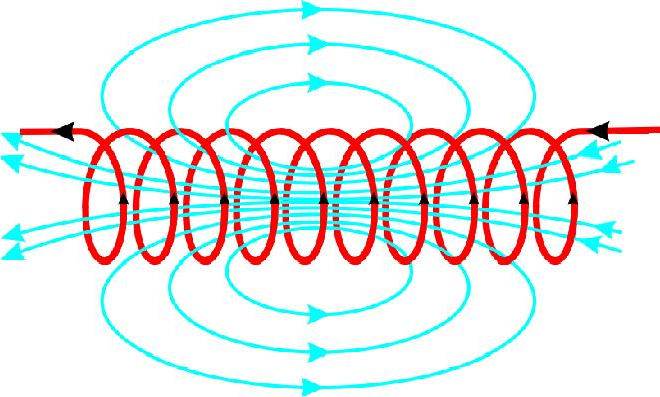
\includegraphics[height=2.5cm]{solenoid_field.png}};
  \node[anchor=south west,text width=8.2cm,font=\small,align=left] at ([xshift=1cm,yshift=0.35cm]current page.south west) {%
    \textbf{Complete classroom deck}: every derivation worked step by step with reasons, labelled diagrams, solved numericals, all textbook questions.\\[4pt]
    \textcolor{gray}{Figures: SCERT Class X Physical Science textbook, pp.\,219--248}};
\end{tikzpicture}
\end{frame}

% =====================================================================
\begin{frame}{Chapter roadmap}
\begin{columns}[T]
\column{0.5\textwidth}
\begin{tcolorbox}[colback=emblue!6,colframe=emblue,title={\textbf{Part A: Currents make magnetic fields}}]
\small
\begin{enumerate}
\item[10.1] Oersted experiment
\item[10.2] Magnetic field, field lines, flux $\Phi$, flux density $B$
\item[10.3] Field of a straight wire, circular coil, solenoid
\end{enumerate}
\end{tcolorbox}
\begin{tcolorbox}[colback=empurple!6,colframe=empurple,title={\textbf{Part B: Fields push on currents}}]
\small
\begin{enumerate}
\item[10.4] $F=qvB\sin\theta$, $F=ILB\sin\theta$, circular motion
\item[10.4] Electric motor
\end{enumerate}
\end{tcolorbox}
\column{0.5\textwidth}
\begin{tcolorbox}[colback=emgreen!6,colframe=emgreen,title={\textbf{Part C: Changing fields make currents}}]
\small
\begin{enumerate}
\item[10.5] Electromagnetic induction
\item[10.5] Faraday's law, Lenz's law
\item[10.5] Derivation: motional emf $\varepsilon=Blv$
\item[10.5] Applications, magnetic levitation
\item[10.5] AC and DC generators
\end{enumerate}
\end{tcolorbox}
\begin{examtip}[How to use this deck]
\small Badges \badge{1M} \badge{2M} \badge{4M} show usual marks. \textbf{Derivation} frames show \emph{step, working, reason}. Answers to \textbf{Teacher asks} appear on the next click.
\end{examtip}
\end{columns}
\end{frame}

% =====================================================================
\begin{frame}{Recall and warm-up}
\begin{columns}[c]
\column{0.52\textwidth}
\begin{itemize}
\item A magnet has two poles, N and S. Like poles repel, unlike poles attract.
\item A freely suspended magnet (compass needle) rests along the \textbf{north--south} direction.
\item A \textbf{field force} acts without contact (gravity, electric, magnetic).
\item Electric current = charges in motion: $I=\dfrac{Q}{t}$.
\item Electric power $P=\varepsilon I$; work $W=Fs$; power $P=Fv$.
\end{itemize}
\column{0.45\textwidth}
\begin{think}[Warm-up questions]
\small
\begin{itemize}
\item How do electric motors and calling bells work?
\item How does an electromagnet work?
\item Is there any relation between electricity and magnetism?
\item Can we produce electricity from magnetism?
\end{itemize}
\end{think}
\end{columns}
\end{frame}

% =====================================================================

\section{Basics first}

% =====================================================================
\begin{frame}{The big picture: one story in three steps}
\centering
\begin{tikzpicture}
\node[story=emblue] (a) at (-5.4,0) {\textbf{\faBolt\ Electric current}\\ moving charges};
\node[story=emteal] (b) at (0,0) {\textbf{\faMagnet\ Magnetic field}\\ appears around the current};
\node[story=emorange] (c) at (5.4,0) {\textbf{\faCog\ Motion}\\ the field pushes things};
\draw[-{Stealth},very thick,emblue] (a) -- node[above,font=\footnotesize,align=center]{\textbf{Part A}\\Oersted} (b);
\draw[-{Stealth},very thick,empurple] (b) -- node[above,font=\footnotesize,align=center]{\textbf{Part B}\\Motor} (c);
\draw[-{Stealth},very thick,emgreen,rounded corners=8pt] (c.south) -- ++(0,-1.3) -- node[below,font=\footnotesize]{\textbf{Part C}: moving a magnet makes current again (Generator)} ($(a.south)+(0,-1.3)$) -- (a.south);
\end{tikzpicture}
\vspace{6pt}
\begin{simple}[Remember this one line]
Electricity and magnetism are \textbf{two faces of the same thing}. Current makes magnetism; magnetism pushes current; changing magnetism makes current.
\end{simple}
\end{frame}
% =====================================================================
\begin{frame}{Basics 1: What is a magnet?}
\begin{columns}[c]
\column{0.5\textwidth}\centering
\begin{tikzpicture}[scale=0.85]
\foreach \y/\l/\r in {1.6/N/S,0.4/S/N,-0.8/N/N}{
 \ifx\l N \def\cl{emred}\else\def\cl{emblue}\fi
 \ifx\r N \def\cr{emred}\else\def\cr{emblue}\fi
 \fill[\cl] (-2.6,\y) rectangle (-1.3,\y+0.55); \node[white,font=\bfseries] at (-1.95,\y+0.27) {\l};
 \fill[\cr] (1.3,\y) rectangle (2.6,\y+0.55); \node[white,font=\bfseries] at (1.95,\y+0.27) {\r};}
\draw[-{Stealth},thick,emgreen] (-1.0,1.87) -- (-0.1,1.87); \draw[-{Stealth},thick,emgreen] (1.0,1.87) -- (0.1,1.87);
\node[font=\small\bfseries,emgreen!60!black] at (0,1.5) {attract};
\draw[-{Stealth},thick,emgreen] (-1.0,0.67) -- (-0.1,0.67); \draw[-{Stealth},thick,emgreen] (1.0,0.67) -- (0.1,0.67);
\node[font=\small\bfseries,emgreen!60!black] at (0,0.3) {attract};
\draw[-{Stealth},thick,emred] (-0.1,-0.53) -- (-1.0,-0.53); \draw[-{Stealth},thick,emred] (0.1,-0.53) -- (1.0,-0.53);
\node[font=\small\bfseries,emred] at (0,-0.9) {repel};
\end{tikzpicture}
\column{0.48\textwidth}
\begin{itemize}
\item Every magnet has \textbf{two poles}: North (N) and South (S).
\item \textbf{Unlike} poles attract. \textbf{Like} poles repel.
\item You can never get a single pole: cut a magnet and each piece has both N and S.
\item Magnets attract iron, nickel and cobalt.
\end{itemize}
\begin{simple}[Think of it like this]
A \textbf{compass needle} is a tiny magnet. Its N end always swings to the Earth's geographic north because the Earth itself acts like a giant magnet.
\end{simple}
\end{columns}
\end{frame}
% =====================================================================
\begin{frame}{Basics 2: What is a ``field''?}
\begin{columns}[c]
\column{0.5\textwidth}
\begin{simple}[Kitchen smell analogy]
Cooking in a kitchen: you smell it \textbf{without touching} the food.
\begin{itemize}
\item Strong smell near the stove; weak far away $\Rightarrow$ \textbf{strength} changes with place.
\item Smell drifts \emph{from} the stove \emph{towards} you $\Rightarrow$ it has a \textbf{direction}.
\end{itemize}
\end{simple}
\begin{defn}[Field]
\small Space around an object where it can push or pull other things \textbf{without touching}. A field has \key{strength} and \key{direction} at every point.
\end{defn}
\column{0.46\textwidth}\centering
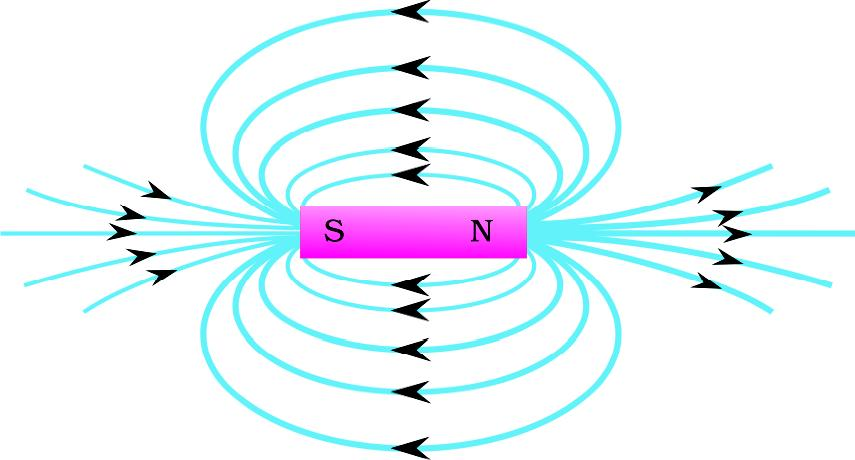
\includegraphics[width=0.95\linewidth]{bar_field.png}\\
{\scriptsize Magnetic field of a bar magnet. Each curve is a \textbf{field line}: the arrow shows the direction; crowded lines mean a stronger field.}
\end{columns}
\end{frame}
% =====================================================================
\begin{frame}{Basics 3: What is electric current?}
\begin{columns}[c]
\column{0.5\textwidth}\centering
\begin{tikzpicture}
\draw[very thick] (0,0) -- (1.7,0) (2.5,0) -- (4.4,0) -- (4.4,0.9) (4.4,1.5) -- (4.4,2.4) -- (0,2.4) -- (0,0);
\draw[very thick] (1.7,-0.4) -- (1.7,0.4); \draw[ultra thick] (2.5,-0.22) -- (2.5,0.22);
\node[font=\footnotesize] at (1.7,-0.75) {$+$}; \node[font=\footnotesize] at (2.5,-0.75) {$-$};
\node[font=\footnotesize] at (2.1,-1.2) {battery};
\fill[yellow!70,draw=black,thick] (4.4,1.2) circle (0.3); \node[font=\footnotesize,anchor=west] at (4.75,1.2) {bulb};
\draw[cur] (1.1,2.4) -- (3.3,2.4) node[midway,above=3pt,font=\footnotesize,emred]{current $I$ drawn $+\to-$};
\foreach \x in {0.5,1.3,2.1,2.9,3.7}\fill[emblue] (\x,0) circle (2.5pt);
\draw[-{Stealth},emblue,thick] (3.8,0.45) -- (0.6,0.45);
\node[font=\footnotesize,emblue] at (2.2,0.8) {electrons really go this way};
\end{tikzpicture}
\column{0.48\textwidth}
\begin{itemize}
\item Current is the \textbf{flow of charge}, like water flowing in a pipe.
\item Battery = pump, wire = pipe, charge = water.
\end{itemize}
\begin{formula}[Current]
\[I=\frac{Q}{t}\quad\text{unit: ampere (A)}\]
\small $1\,\text{A}=1$ coulomb of charge per second.
\end{formula}
\begin{simple}[Direction convention]
We \textbf{draw} current from $+$ to $-$ (old convention). Electrons really go the other way. Always follow the \textbf{drawn} direction in this chapter.
\end{simple}
\end{columns}
\end{frame}
% =====================================================================
\begin{frame}{Basics 4: Reading arrows into and out of the page}
\begin{columns}[c]
\column{0.5\textwidth}\centering
\begin{tikzpicture}
% dart side view
% toward you
\node[font=\footnotesize,align=center] at (0.2,0.2) {\textbf{towards you}\\you see the \textbf{tip}};
\draw[thick,fill=white] (2.4,0.2) circle (0.4); \fill (2.4,0.2) circle (0.1);
\node[font=\Large\bfseries,emred] at (3.5,0.2) {$\odot$};
% away
\node[font=\footnotesize,align=center] at (0.2,-1.5) {\textbf{away from you}\\you see the \textbf{tail feathers}};
\draw[thick,fill=white] (2.4,-1.5) circle (0.4); \draw[thick] (2.4-0.28,-1.5-0.28)--(2.4+0.28,-1.5+0.28) (2.4-0.28,-1.5+0.28)--(2.4+0.28,-1.5-0.28);
\node[font=\Large\bfseries,emblue] at (3.5,-1.5) {$\otimes$};
\end{tikzpicture}
\column{0.48\textwidth}
\begin{itemize}
\item $\odot$ (dot) $\Rightarrow$ pointing \textbf{out of the page}, towards you.
\item $\otimes$ (cross) $\Rightarrow$ pointing \textbf{into the page}, away from you.
\item A page full of $\times$ means a magnetic field going \textbf{into} the page; full of $\cdot$ means \textbf{out}.
\end{itemize}
\begin{simple}[Memory trick]
\textbf{D}ot = \textbf{D}ooming at you (the \emph{tip} is coming at you).\\ \textbf{C}ross = \textbf{C}arrying away (you see the \emph{tail}, it is leaving).
\end{simple}
\end{columns}
\end{frame}
% =====================================================================
\begin{frame}{Basics 5: Your right hand is the tool of this chapter}
\begin{columns}[T]
\column{0.33\textwidth}\centering
\textbf{\color{emblue}Rule 1: thumb rule}\\[2pt]
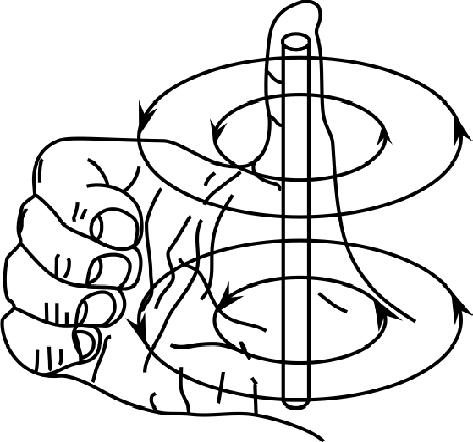
\includegraphics[height=2.4cm]{thumb_rule.png}\\
{\small Straight wire.\\ \textbf{Thumb} = current.\\ \textbf{Curled fingers} = field.}
\column{0.33\textwidth}\centering
\textbf{\color{emteal}Rule 2: coil rule}\\[2pt]
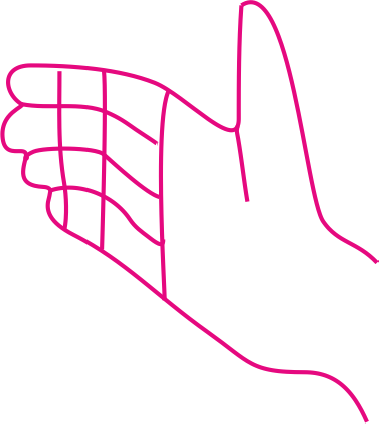
\includegraphics[height=2.4cm]{coil_hand.png}\\
{\small Coil or solenoid.\\ \textbf{Curled fingers} = current.\\ \textbf{Thumb} = N pole.}
\column{0.33\textwidth}\centering
\textbf{\color{emorange}Rule 3: force rule}\\[2pt]

\includegraphics[height=2.4cm]{rh_rule_b.png}\\
{\small Force on current/charge.\\ \textbf{Forefinger} = current $I$ (or $v$),\\ \textbf{middle finger} = field $B$,\\ \textbf{thumb} = force $F$.}
\end{columns}
\vspace{4pt}
\begin{simple}[Always ask: ``What do I know, and what do I want?'']
Know the \textbf{current}, want the \textbf{field}? Rule 1 or 2. Know the \textbf{current and field}, want the \textbf{push}? Rule 3. Use your \textbf{right} hand only.
\end{simple}
\end{frame}
% =====================================================================
\begin{frame}{Basics 6: Symbols and units you will meet}
\centering\renewcommand{\arraystretch}{1.25}
\begin{tabular}{@{}llll@{}}
\toprule
\textbf{Quantity} & \textbf{Symbol} & \textbf{SI unit} & \textbf{In plain words}\\
\midrule
Electric current & $I$ & ampere (A) & how fast charge flows\\
Charge & $q$ or $Q$ & coulomb (C) & amount of electric charge\\
Velocity & $v$ & m/s & speed with direction\\
Magnetic flux density & $B$ & tesla (T) & strength of the field\\
Magnetic flux & $\Phi$ & weber (Wb) & total field passing through an area\\
Force & $F$ & newton (N) & a push or pull\\
Induced emf & $\varepsilon$ & volt (V) & electrical ``push'' that drives current\\
\bottomrule
\end{tabular}
\vspace{4pt}
\begin{examtip}[Unit tip]
$1\,\text{T}=1\,\text{Wb/m}^2$. Convert first: cm $\to$ m, cm$^2\to$ m$^2$ (divide by $10^4$), before substituting into formulas.
\end{examtip}
\end{frame}
% =====================================================================
\begin{frame}{Maths 1: Powers of ten (scientific notation)}
\begin{columns}[T]
\column{0.5\textwidth}
\begin{simple}[Why?]
Physics numbers can be huge or tiny. Charge of a proton: $0.00000000000000000016$ C. Write it as $\mathbf{1.6\times10^{-19}}$ C.
\end{simple}
\begin{itemize}
\item $10^{3}=1000$,\; $10^{-3}=\dfrac{1}{1000}=0.001$
\item Move the point \textbf{left} $\Rightarrow$ power goes \textbf{up}; move \textbf{right} $\Rightarrow$ power goes \textbf{down}.
\end{itemize}
\column{0.48\textwidth}
\begin{formula}[Rules]
\[10^{a}\times10^{b}=10^{a+b}\qquad\frac{10^{a}}{10^{b}}=10^{a-b}\]
\end{formula}
\begin{answer}[Worked example]
$(2\times10^{6})\times(1.6\times10^{-19})\times0.5$\\
Numbers: $2\times1.6\times0.5=1.6$\\
Powers: $10^{6-19}=10^{-13}$\\
Answer: $\mathbf{1.6\times10^{-13}}$
\end{answer}
\end{columns}
\end{frame}
% =====================================================================
\begin{frame}{Maths 2: Changing units before you calculate}
\centering\renewcommand{\arraystretch}{1.25}
\begin{tabular}{@{}lll@{}}
\toprule
\textbf{Change} & \textbf{How} & \textbf{Example}\\
\midrule
cm $\to$ m & divide by 100 & $20\ \text{cm}=0.2$ m\\
mm $\to$ m & divide by 1000 & $5.7$ mm $=5.7\times10^{-3}$ m\\
cm$^2\to$ m$^2$ & divide by $10^{4}$ (not 100!) & $4\ \text{cm}^2=4\times10^{-4}$ m$^2$\\
minutes $\to$ s & multiply by 60 & $0.2$ min $=12$ s\\
\bottomrule
\end{tabular}
\vspace{6pt}
\begin{simple}[Why $10^4$ for area?]
$1\ \text{cm}=\frac{1}{100}$ m, so $1\ \text{cm}^2=\frac{1}{100}\times\frac{1}{100}=\frac{1}{10\,000}$ m$^2$. Area squares the conversion factor.
\end{simple}
\end{frame}
% =====================================================================
\begin{frame}{Maths 3: Rearranging a formula (the balance method)}
\begin{columns}[T]
\column{0.5\textwidth}
\begin{simple}[Golden rule]
An equation is a balance. Whatever you do to one side, do the \textbf{same} to the other.
\end{simple}
Start with $F=ILB$.
\begin{itemize}
\item Find $B$: divide both sides by $IL$ $\Rightarrow$ $B=\dfrac{F}{IL}$
\item Find $I$: divide both sides by $LB$ $\Rightarrow$ $I=\dfrac{F}{LB}$
\item Find $L$: divide both sides by $IB$ $\Rightarrow$ $L=\dfrac{F}{IB}$
\end{itemize}
\column{0.48\textwidth}
\begin{answer}[Example from the chapter]
$r=\dfrac{mv}{Bq}$. Find $v$.\\[3pt]
Multiply both sides by $Bq$: $rBq=mv$\\
Divide both sides by $m$: $v=\dfrac{rBq}{m}$
\end{answer}
\begin{examtip}[Steps for every numerical]
1. Write the formula. 2. Convert units. 3. Rearrange if needed. 4. Substitute. 5. Calculate and write the \textbf{unit}.
\end{examtip}
\end{columns}
\end{frame}
% =====================================================================
\begin{frame}{Maths 4: Sine and cosine of an angle}
\begin{columns}[c]
\column{0.42\textwidth}\centering
\begin{tikzpicture}[scale=0.95]
\draw[thick] (0,0) -- (2.6,0) -- (2.6,1.5) -- cycle;
\draw[thick] (2.45,0) -- (2.45,0.15) -- (2.6,0.15);
\draw (0.6,0) arc (0:30:0.6); \node[font=\small] at (0.85,0.17) {$\theta$};
\node[font=\small,emblue] at (1.3,-0.3) {adjacent};
\node[font=\small,emred,rotate=90] at (2.95,0.75) {opposite};
\node[font=\small,emteal,rotate=30] at (1.15,1.0) {hypotenuse};
\end{tikzpicture}
{\small$\sin\theta=\dfrac{\text{opposite}}{\text{hypotenuse}}$\\[4pt]$\cos\theta=\dfrac{\text{adjacent}}{\text{hypotenuse}}$}
\column{0.56\textwidth}
\small\centering\renewcommand{\arraystretch}{1.2}
\begin{tabular}{@{}c|ccccc@{}}
$\theta$ & $0^\circ$ & $30^\circ$ & $45^\circ$ & $60^\circ$ & $90^\circ$\\\hline
$\sin\theta$ & $0$ & $\tfrac12$ & $\tfrac{1}{\sqrt2}$ & $\tfrac{\sqrt3}{2}$ & $1$\\
$\cos\theta$ & $1$ & $\tfrac{\sqrt3}{2}$ & $\tfrac{1}{\sqrt2}$ & $\tfrac12$ & $0$\\
\end{tabular}
\vspace{4pt}
\begin{simple}[Where we use them]
$F=qvB\sin\theta$: $\theta$ is the angle between $v$ and $B$. At $90^\circ$ the force is maximum; at $0^\circ$ it is zero.\\
$\Phi=BA\cos\theta$: $\theta$ is the angle between $B$ and the \textbf{normal} to the plane. At $0^\circ$ the flux is maximum.
\end{simple}
\end{columns}
\end{frame}
% =====================================================================
\begin{frame}{Maths 5: Area, circles and time period}
\begin{columns}[T]
\column{0.5\textwidth}
\begin{formula}[Shapes]
\small Rectangle: $A=\text{length}\times\text{breadth}$\\
Circle: $A=\pi r^{2}$, circumference $=2\pi r$ ($\pi\approx3.14$)
\end{formula}
\begin{answer}[Example]
Loop of radius $0.1$ m: $A=3.14\times0.1^{2}=0.0314$ m$^{2}$.
\end{answer}
\column{0.48\textwidth}
\begin{formula}[Speed, distance, time]
\[v=\frac{\text{distance}}{\text{time}}\;\Rightarrow\;\text{time}=\frac{\text{distance}}{v}\]
\end{formula}
\begin{simple}[Time period $T$]
Time for one full circle: $T=\dfrac{2\pi r}{v}$. We use this in the circular-path derivation.
\end{simple}
\end{columns}
\end{frame}
% =====================================================================
\begin{frame}{Maths 6: ``Change'' and ``rate of change'' ($\Delta$)}
\begin{columns}[c]
\column{0.5\textwidth}
\begin{itemize}
\item $\Delta$ (delta) means \textbf{change} = final $-$ initial.
\item $\Delta\Phi=\Phi_{\text{final}}-\Phi_{\text{initial}}$,\quad $\Delta t=t_{\text{final}}-t_{\text{initial}}$
\item \textbf{Rate of change} = change $\div$ time taken, e.g.\ $\varepsilon=\dfrac{\Delta\Phi}{\Delta t}$.
\end{itemize}
\begin{answer}[Example]
Flux falls from $0.5$ Wb to $0.1$ Wb in $0.2$ s.\\
$\Delta\Phi=0.1-0.5=-0.4$ Wb\\
$|\varepsilon|=\dfrac{0.4}{0.2}=\mathbf{2}$ V
\end{answer}
\column{0.46\textwidth}\centering
\begin{tikzpicture}[scale=0.85]
\draw[-{Stealth}] (0,0) -- (4.2,0) node[right,font=\small]{$t$ (s)};
\draw[-{Stealth}] (0,0) -- (0,3) node[above,font=\small]{$\Phi$ (Wb)};
\draw[very thick,emblue] (0,2.5) -- (3.2,0.5);
\draw[dashed] (0,2.5) -- (3.2,2.5) -- (3.2,0.5);
\node[font=\small] at (1.6,2.8) {$\Delta t$}; \node[font=\small,anchor=west] at (3.25,1.5) {$\Delta\Phi$};
\end{tikzpicture}\\
{\small Slope of a flux--time graph = $\dfrac{\Delta\Phi}{\Delta t}$ = induced emf. A steeper line means a bigger emf; a flat line means zero emf.}
\end{columns}
\end{frame}
% =====================================================================
\begin{frame}{Maths 7: Proportion, ``if this doubles, what happens?''}
\begin{columns}[T]
\column{0.55\textwidth}
\renewcommand{\arraystretch}{1.3}\small
\begin{tabular}{@{}lll@{}}
\toprule
\textbf{Formula} & \textbf{If this doubles\ldots} & \textbf{That}\\
\midrule
$F=ILB$ & $B$ doubles & $F$ doubles\\
$F=ILB$ & $I$ and $L$ both double & $F$ becomes $4\times$\\
$r=\dfrac{mv}{Bq}$ & $B$ doubles & $r$ \textbf{halves}\\
$\varepsilon=Blv$ & $v$ doubles & $\varepsilon$ doubles\\
$\Phi=BA\cos\theta$ & $A$ doubles & $\Phi$ doubles\\
\bottomrule
\end{tabular}
\column{0.43\textwidth}
\begin{simple}[Two kinds of relation]
\textbf{Direct} ($F\propto B$): both grow together.\\
\textbf{Inverse} ($r\propto\frac{1}{B}$): one grows, the other shrinks.
\end{simple}
\begin{examtip}
Spot the variable on top (direct) or underneath (inverse) in the formula.
\end{examtip}
\end{columns}
\end{frame}
% =====================================================================
\begin{frame}{Maths check: try these}
\small
\begin{columns}[T]
\column{0.5\textwidth}
\begin{think}[Quick maths drill]
\begin{enumerate}
\item Write $0.0005$ in powers of ten.
\item Convert $50$ cm$^2$ to m$^2$.
\item $F=ILB$: find $L$ if $F=6$ N, $I=3$ A, $B=0.5$ T.
\item Value of $\sin30^\circ$ and $\cos60^\circ$?
\item Flux changes by $0.6$ Wb in $0.3$ s. Find $\varepsilon$.
\end{enumerate}
\end{think}
\column{0.46\textwidth}
\uncover<2->{\begin{answer}[Answers]
\begin{enumerate}
\item $5\times10^{-4}$
\item $5\times10^{-3}$ m$^2$
\item $L=\dfrac{6}{3\times0.5}=4$ m
\item both $\tfrac12$
\item $\varepsilon=\dfrac{0.6}{0.3}=2$ V
\end{enumerate}
\end{answer}}
\end{columns}
\end{frame}
% =====================================================================
\begin{frame}{Quick check before we start}
\small
\begin{columns}[T]
\column{0.5\textwidth}
\begin{think}[Try these (answers on the next click)]
\begin{enumerate}
\item Two N poles are brought close. Attract or repel?
\item Charge $6$ C flows in $2$ s. Find the current.
\item An arrow shows $\otimes$. Is it going into or out of the page?
\item Which hand do we use for the rules?
\end{enumerate}
\end{think}
\column{0.46\textwidth}
\uncover<2->{\begin{answer}[Answers]
\begin{enumerate}
\item Repel (like poles).
\item $I=Q/t=6/2=3$ A.
\item Into the page.
\item The right hand.
\end{enumerate}
\end{answer}}
\end{columns}
\end{frame}

\section{Part A: Magnetic field}
% =====================================================================
\begin{frame}{Part A: Currents make magnetic fields}
\begin{goals}
\large\begin{itemize}
\item Describe what Oersted observed and what it proves.
\item Draw and read \textbf{magnetic field lines}; tell a strong field from a weak one.
\item Explain \textbf{flux} $\Phi$ and \textbf{flux density} $B$, and use $\Phi=BA\cos\theta$.
\item Find the field direction around a wire, a coil and a solenoid with the \textbf{right hand rule}.
\end{itemize}
\end{goals}
\end{frame}

\begin{frame}{10.1 Oersted experiment (Activity 1) \hfill \badge{2M} \badge{4M}}
\begin{columns}[T]
\column{0.56\textwidth}
\centering
\figlab{oersted_setup.png}{width=\linewidth}{
\draw[fptr] (0.30,1.12) node[flab,anchor=south east]{copper wire (24 gauge)} -- (0.36,0.82);
\draw[fptr] (0.36,1.12) node[flab,anchor=south west]{wooden sticks} -- (0.50,0.95);
\draw[fptr] (0.36,1.12) -- (0.27,0.62);
\draw[fptr] (0.30,0.20) node[flab,anchor=north]{magnetic compass} -- (0.40,0.60);
\draw[fptr] (0.85,1.10) node[flab,anchor=south]{battery (3 V)} -- (0.66,0.78);
\draw[fptr] (0.72,0.10) node[flab,anchor=north]{key} -- (0.54,0.40);
\draw[fptr] (0.05,0.05) node[flab,anchor=north]{thermocol sheet} -- (0.15,0.40);}\\[12pt]
{\scriptsize fig-1: current-carrying wire above a compass}
\column{0.42\textwidth}
\small
\begin{enumerate}
\item Wire stretched through slits of two sticks, in series with battery and key. Compass below the wire.
\item Bring a bar magnet near: needle deflects (magnetic force).
\item Remove the magnet, switch \textbf{on}: needle \textbf{deflects again}!
\item Switch off: needle returns to N--S.
\end{enumerate}
\begin{answer}[Conclusion]
\small A \textbf{current-carrying wire produces a magnetic field} around it. Electricity and magnetism are related.
\end{answer}
\end{columns}
\end{frame}

% =====================================================================
\begin{frame}{Do you know? Hans Christian Oersted \hfill \badge{1M}}
\begin{columns}[c]
\column{0.26\textwidth}\centering
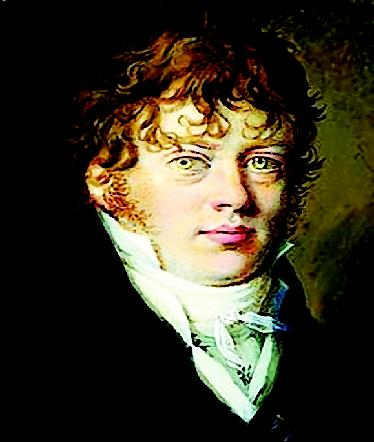
\includegraphics[width=0.9\linewidth]{oersted.png}\\{\scriptsize H.\,C.\ Oersted (1777--1851)}
\column{0.72\textwidth}
\begin{itemize}
\item In a lecture in April 1820 he placed a compass needle under a wire and switched on the current: the needle \textbf{deflected}.
\item Showed that electricity and magnetism are \textbf{interconnected}: the start of \key{electromagnetism}.
\item Led to the dynamo, the electric motor, radio, television and fibre optics.
\item The unit of magnetic field strength is named \imp{oersted} in his honour.
\end{itemize}
\end{columns}
\end{frame}

% =====================================================================
\begin{frame}{10.2 Magnetic field of a bar magnet (Activity 2) \hfill \badge{1M} \badge{2M}}
\begin{columns}[T]
\column{0.55\textwidth}
\begin{activity}[Activity 2: compass around a bar magnet]
\small Place a compass at many points around a bar magnet on paper. Mark the direction of the needle at each point (S $\to$ N of the needle).
\end{activity}
\small
\begin{itemize}
\item The needle points in \textbf{different directions} at different places $\Rightarrow$ the field has \textbf{direction} that varies from point to point.
\item Far from the magnet the needle points almost N--S $\Rightarrow$ \textbf{strength} decreases with distance.
\item Above the magnet the needle is also deflected $\Rightarrow$ the field is \textbf{three-dimensional}.
\end{itemize}
\column{0.43\textwidth}
\begin{defn}[Field]
\small A region where a force acts on an object \textbf{without physical contact}.
\end{defn}
\begin{defn}[Magnetic field]
\small The region surrounding a magnet in which its magnetic force can be felt. It is characterised by \key{strength} and \key{direction}.
\end{defn}
\end{columns}
\end{frame}

% =====================================================================
\begin{frame}{10.2.1 Magnetic field lines (Activity 3) \hfill \badge{1M} \badge{2M} \badge{Diagram}}
\begin{columns}[c]
\column{0.5\textwidth}\centering
\figlab{bar_field.png}{width=\linewidth}{
\draw[fptr] (0.12,1.08) node[flab,anchor=south]{field line} -- (0.30,0.93);
\draw[fptr] (0.88,1.08) node[flab,anchor=south]{lines crowded near poles (strong)} -- (0.72,0.62);
\draw[fptr] (0.50,-0.10) node[flab,anchor=north]{lines far apart (weak)} -- (0.50,0.04);}\\[12pt]
{\scriptsize fig-2: field lines of a bar magnet (outside: N $\to$ S)}
\column{0.48\textwidth}
\small
\textbf{Plotting:} put the compass at N, mark a dot at the tip of the needle, move the compass to the dot, repeat until you reach S. Join the dots.
\begin{itemize}
\item Field lines are \textbf{imaginary} curves.
\item \key{Tangent} at any point gives the direction of the field.
\item \textbf{Crowded} lines $\Rightarrow$ strong field; \textbf{spread} lines $\Rightarrow$ weak field.
\item \key{Non-uniform field}: strength \textbf{or} direction changes.\\ \key{Uniform field}: strength \textbf{and} direction constant (parallel, equally spaced lines).
\end{itemize}
\end{columns}
\end{frame}

% =====================================================================
\begin{frame}{10.2.2 Magnetic flux and flux density \hfill \badge{1M} \badge{2M}}
\begin{columns}[c]
\column{0.44\textwidth}\centering
\begin{tikzpicture}[scale=0.9]
\foreach \y in {-1.2,-0.6,0,0.6,1.2} \draw[fl=0.2] (-2.2,\y) -- (2.4,\y);
\fill[gray!35,opacity=0.8] (0,0) ellipse (0.28 and 1.05);
\draw[thick] (0,0) ellipse (0.28 and 1.05);
\node[flab] at (0.0,-1.6) {plane of area $A$};
\node[font=\small\bfseries,fieldc] at (-2.5,0.9) {$B$};
\node[font=\scriptsize,align=center] at (1.5,1.65) {plane $\perp$ field};
\end{tikzpicture}\\
{\scriptsize fig-3(a): lines crossing a plane placed perpendicular to a uniform field}
\column{0.54\textwidth}
\begin{defn}[Magnetic flux $\Phi$]
\small The number of field lines passing through a plane of area $A$ held \textbf{perpendicular} to the field. SI unit: \key{weber (Wb)}.
\end{defn}
\begin{defn}[Magnetic flux density $B$]
\small Flux passing through \textbf{unit area} held perpendicular to the field. Also called \key{magnetic induction}.
\[B=\frac{\Phi}{A}\qquad\text{unit: Wb/m}^2=\text{tesla (T)}\]
\end{defn}
\end{columns}
\end{frame}

% =====================================================================
\begin{frame}[shrink=8]{Flux in simple words: rain through a window}
\begin{columns}[c]
\column{0.6\textwidth}\centering
\begin{tikzpicture}[scale=0.6]
\foreach \ang/\xo/\lab in {90/0/{face-on: \textbf{most} lines},60/4.2/{tilted: \textbf{fewer}},0/8.4/{edge-on: \textbf{none}}}{
 \foreach \y in {-1.0,-0.5,0,0.5,1.0} \draw[fl=0.3] (\xo-1.2,\y) -- (\xo+1.2,\y);
 \draw[very thick,emorange] ($(\xo,0)+(\ang:1.3)$) -- ($(\xo,0)-(\ang:1.3)$);
 \node[font=\footnotesize,align=center] at (\xo,-1.8) {\lab};}
\end{tikzpicture}\\
{\scriptsize Orange line = the window seen edge-on; blue lines = field lines (rain).}
\column{0.38\textwidth}
\begin{simple}[Analogy]
Rain = field lines. Window = area $A$.
\begin{itemize}
\item Hold the window \textbf{face-on}: the most rain passes.
\item \textbf{Tilt} it: less passes.
\item \textbf{Edge-on}: no rain passes.
\end{itemize}
\textbf{Flux $\Phi$} = how much rain passes. \textbf{Flux density $B$} = how heavy the rain is.
\end{simple}
\end{columns}
\end{frame}

% =====================================================================
\begin{frame}[shrink=15]{Derivation 1: flux through a tilted plane, $\Phi=BA\cos\theta$ \hfill \badge{2M}}
\begin{columns}[T]
\column{0.4\textwidth}\centering
\begin{tikzpicture}[scale=0.95]
\foreach \y in {0.2,0.7,1.2,1.7,2.2} \draw[fl=0.15] (-0.5,\y) -- (3.8,\y);
\node[font=\small\bfseries,fieldc] at (-0.75,2.2) {$B$};
% tilted plane (edge view)
\draw[very thick,emorange] (1.2,0.1) -- (2.2,2.4);
\node[flab,anchor=west] at (2.25,2.5) {plane, area $A$};
% normal
\coordinate (C) at (1.7,1.25);
\draw[-{Stealth},thick,empurple] (C) -- ($(C)+(-23.5:1.3)$) node[below right,font=\scriptsize,empurple,fill=white,inner sep=1pt]{normal};
\draw[dashed,gray] (C) -- ($(C)+(1.3,0)$);
\draw[empurple] ($(C)+(0.6,0)$) arc (0:-23.5:0.6); \node[font=\scriptsize,empurple] at ($(C)+(-12:0.85)$) {$\theta$};
% projection perpendicular to field
\draw[thick,dashed,emgreen!70!black] (1.2,0.1) -- (1.2,2.4);
\node[font=\scriptsize,emgreen!60!black,align=center] at (0.55,-0.35) {effective area\\$A\cos\theta$ ($\perp$ field)};
\end{tikzpicture}\\
{\scriptsize fig-3(b): edge view of the plane}
\column{0.58\textwidth}
\begin{steps}[3.3cm]
\stp1 & B=\frac{\Phi}{A_{\perp}} & $B$ is always defined with the area \textbf{perpendicular} to the field\\
\stp2 & A_{\perp}=A\cos\theta & $\theta$ = angle between $B$ and the normal; only this part of the plane faces the field\\
\stp3 & B=\frac{\Phi}{A\cos\theta} & substitute step 2 in step 1\\
\stp4 & \Phi=BA\cos\theta & multiply both sides by $A\cos\theta$\\
\end{steps}
\begin{formula}[Special cases]
\small $\theta=0^\circ$ (plane $\perp$ field): $\Phi=BA$ (maximum)\\
$\theta=90^\circ$ (plane $\parallel$ field): $\Phi=BA\cos90^\circ=0$
\end{formula}
\end{columns}
\end{frame}

% =====================================================================
\begin{frame}{Solved numericals: flux and flux density \hfill \badge{2M}}
\small
\begin{columns}[T]
\column{0.5\textwidth}
\begin{tcolorbox}[colback=emblue!4,colframe=emblue,title={\textbf{Q1.} $B=0.5$ T through a loop of area $0.02$ m$^2$, loop $\perp$ field. Find $\Phi$.}]
\stp1 Plane $\perp$ field $\Rightarrow\theta=0^\circ$, $\cos0^\circ=1$.\\
\stp2 $\Phi=BA=0.5\times0.02=\boxed{0.01\ \text{Wb}}$
\end{tcolorbox}
\pause
\begin{tcolorbox}[colback=emblue!4,colframe=emblue,title={\textbf{Q2.} Same loop turned so the normal makes $60^\circ$ with $B$.}]
\stp1 $\Phi=BA\cos60^\circ=0.01\times\frac12=\boxed{0.005\ \text{Wb}}$
\end{tcolorbox}
\column{0.5\textwidth}
\pause
\begin{tcolorbox}[colback=emgreen!5,colframe=emgreen,title={\textbf{Q3.} Flux of $2\times10^{-3}$ Wb crosses $4$ cm$^2$ normally. Find $B$.}]
\stp1 $A=4\ \text{cm}^2=4\times10^{-4}$ m$^2$ \;(1 cm$^2=10^{-4}$ m$^2$)\\[2pt]
\stp2 $B=\dfrac{\Phi}{A}=\dfrac{2\times10^{-3}}{4\times10^{-4}}=\boxed{5\ \text{T}}$
\end{tcolorbox}
\pause
\begin{think}[Textbook question]
\small What is the flux through a plane held \textbf{parallel} to the field?\\
\onslide<5->{\textbf{Zero}: no field line crosses it ($\theta=90^\circ$).}
\end{think}
\end{columns}
\end{frame}

% =====================================================================
\begin{frame}{10.3.1 Field of a straight current-carrying wire (Activity 4) \hfill \badge{2M} \badge{4M}}
\begin{columns}[T]
\column{0.42\textwidth}\centering
\figlab{wire_setup.png}{height=0.6\textheight}{
\draw[fptr] (0.30,0.97) node[flab,anchor=south]{retort stand} -- (0.58,0.92);
\draw[fptr] (1.05,0.97) node[flab,anchor=south]{vertical wire} -- (0.84,0.75);
\draw[fptr] (1.02,0.02) node[flab,anchor=north]{compass needles} -- (0.85,0.51);
\draw[fptr] (0.62,0.02) node[flab,anchor=north]{plank} -- (0.70,0.50);
\draw[fptr] (-0.05,0.70) node[flab,anchor=east]{battery} -- (0.27,0.52);
\draw[fptr] (-0.05,0.45) node[flab,anchor=east]{switch} -- (0.38,0.49);
\draw[fptr] (-0.05,0.25) node[flab,anchor=east]{table} -- (0.10,0.35);}\\
{\scriptsize fig-4(a)}
\column{0.56\textwidth}
\small
\begin{enumerate}
\item Pass a vertical wire through a hole in a plank; place 6--10 compass needles on a circle around the hole.
\item Switch on (3 V battery).
\item The needles set along \textbf{tangents to the circle}.
\item Sprinkle iron filings: they form \textbf{concentric circles}.
\end{enumerate}
\begin{answer}[Conclusion]
\small Field lines of a straight wire are \textbf{concentric circles} centred on the wire, in a plane perpendicular to it. They are \imp{closed loops}. The field is stronger near the wire (circles closer).
\end{answer}
\end{columns}
\end{frame}

% =====================================================================
\begin{frame}[shrink=6]{Direction of the field: right hand thumb rule \hfill \badge{1M} \badge{2M}}
\begin{columns}[c]
\column{0.28\textwidth}\centering
\begin{tikzpicture}[scale=0.8]
\foreach \r/\p in {0.6/0.12,1.1/0.12,1.6/0.12} \draw[fl=\p] (0,0) circle (\r);
\foreach \r/\p in {0.6/0.62,1.1/0.62,1.6/0.62} \draw[fieldc,thick,postaction={decorate},decoration={markings,mark=at position \p with {\arrow{Stealth[length=5pt]}}}] (0,0) circle (\r);
\outpage{(0,0)}
\node[font=\scriptsize,align=center] at (0,-2.0) {current \textbf{out of} page\\field \textbf{anticlockwise}};
\end{tikzpicture}\\{\scriptsize fig-4(b)}
\column{0.28\textwidth}\centering
\begin{tikzpicture}[scale=0.8]
\foreach \r in {0.6,1.1,1.6} \draw[fieldc,thick,postaction={decorate},decoration={markings,mark=at position 0.12 with {\arrowreversed{Stealth[length=5pt]}},mark=at position 0.62 with {\arrowreversed{Stealth[length=5pt]}}}] (0,0) circle (\r);
\inpage{(0,0)}
\node[font=\scriptsize,align=center] at (0,-2.0) {current \textbf{into} page\\field \textbf{clockwise}};
\end{tikzpicture}\\{\scriptsize fig-4(c)}
\column{0.42\textwidth}\centering
\figlab{thumb_rule.png}{width=0.62\linewidth}{
\draw[cur] (0.63,0.80) -- (0.63,1.08) node[above,font=\scriptsize\bfseries,emred]{thumb: current $I$};
\draw[fptr] (1.10,0.55) node[flab,anchor=west,align=left]{fingers:\\field $B$} -- (0.97,0.72);}\\
{\scriptsize fig-4(d)}
\begin{defn}[Right hand thumb rule]
\small Grasp the wire with the right hand with the \textbf{thumb along the current}; the \textbf{curled fingers} give the direction of the field lines.
\end{defn}
\end{columns}
\vspace{2pt}
{\scriptsize Symbols: $\odot$ current/field out of the page (arrow tip);\quad $\otimes$ into the page (arrow tail).}
\end{frame}

% =====================================================================
\begin{frame}{10.3.2 Field of a circular coil (Activity 5) \hfill \badge{2M} \badge{4M}}
\begin{columns}[T]
\column{0.42\textwidth}\centering
\figlab{coil_setup.png}{width=0.95\linewidth}{
\draw[fptr] (0.10,1.08) node[flab,anchor=south]{circular coil (4--5 turns)} -- (0.34,0.90);
\draw[fptr] (0.62,1.08) node[flab,anchor=south]{compass at centre} -- (0.50,0.70);
\draw[fptr] (0.72,-0.06) node[flab,anchor=north]{to current supply} -- (0.88,0.58);
\draw[fptr] (0.72,-0.06) -- (0.64,0.30);}\\[8pt]
{\scriptsize fig-5(a)}
\column{0.56\textwidth}
\small
\begin{itemize}
\item Plot field lines with a compass around the coil.
\item At the centre the needle points \textbf{perpendicular to the plane of the coil}: the field there is along the axis.
\item Bring a compass near one face: its S pole points to the face $\Rightarrow$ that face acts as a \textbf{N pole}.
\end{itemize}
\begin{defn}[Right hand rule for a coil]
\small Curl the right-hand fingers along the \textbf{current}; the \textbf{thumb} gives the direction of the \textbf{field} (points out of the N face).
\end{defn}
\end{columns}
\end{frame}

\begin{frame}{Coil: which face is North? \hfill \badge{1M} \badge{2M}}
\begin{columns}[c]
\column{0.3\textwidth}\centering
\begin{tikzpicture}
\draw[emred,very thick,postaction={decorate},decoration={markings,mark=at position 0.25 with {\arrow{Stealth[length=6pt]}},mark=at position 0.75 with {\arrow{Stealth[length=6pt]}}}] (0,0) circle (1);
\node[font=\small\bfseries] at (0,0) {N};
\node[font=\scriptsize,align=center] at (0,-1.5) {anticlockwise current\\(as you see it)};
\node[font=\scriptsize,align=center,fieldc] at (0,1.45) {$B$ towards you $\odot$};
\end{tikzpicture}
\column{0.3\textwidth}\centering
\begin{tikzpicture}
\draw[emred,very thick,postaction={decorate},decoration={markings,mark=at position 0.25 with {\arrowreversed{Stealth[length=6pt]}},mark=at position 0.75 with {\arrowreversed{Stealth[length=6pt]}}}] (0,0) circle (1);
\node[font=\small\bfseries] at (0,0) {S};
\node[font=\scriptsize,align=center] at (0,-1.5) {clockwise current\\(as you see it)};
\node[font=\scriptsize,align=center,fieldc] at (0,1.45) {$B$ away from you $\otimes$};
\end{tikzpicture}
\column{0.38\textwidth}\centering
\figlab{coil_hand.png}{width=0.52\linewidth}{
\draw[fptr] (1.08,0.95) node[flab,anchor=west]{thumb: $B$} -- (0.70,0.97);
\draw[fptr] (-0.08,0.45) node[flab,anchor=east,align=right]{fingers:\\current $I$} -- (0.12,0.70);}\\
{\scriptsize fig-5(b): right hand rule for a coil}
\begin{examtip}
\small Memory aid: letters \textbf{N} and \textbf{S} drawn with arrows at their ends run anticlockwise and clockwise respectively.
\end{examtip}
\end{columns}
\end{frame}

% =====================================================================
\begin{frame}{10.3.3 Field of a solenoid (Activity 6) \hfill \badge{2M} \badge{4M}}
\begin{columns}[T]
\column{0.4\textwidth}\centering
\figlab{solenoid_setup.png}{height=0.26\textheight}{
\draw[fptr] (0.12,1.08) node[flab,anchor=south]{solenoid (long helix)} -- (0.36,0.84);
\draw[fptr] (0.70,-0.05) node[flab,anchor=north]{to current supply} -- (0.83,0.52);}\\[4pt]
{\scriptsize fig-6(a)}\\[8pt]
\figlab{solenoid_field.png}{height=0.27\textheight}{
\node[font=\small\bfseries,emred] at (-0.04,0.5) {N};
\node[font=\small\bfseries,emred] at (1.04,0.5) {S};
\node[font=\scriptsize\bfseries,emred] at (0.08,0.80) {$I$};
\node[font=\scriptsize\bfseries,emred] at (0.93,0.80) {$I$};
}\\[2pt]
{\scriptsize fig-6(b): field lines (iron filings)}
\column{0.58\textwidth}
\small
\begin{defn}[Solenoid]
\small A long wire wound in a \textbf{close-packed helix}.
\end{defn}
\begin{itemize}
\item Iron filings show a pattern like that of a \textbf{bar magnet}: a solenoid behaves like a bar magnet.
\item One end is N, the other S (find with the right hand rule).
\item Outside: field lines go \textbf{N $\to$ S}; inside: \textbf{S $\to$ N}, strong and nearly uniform (parallel lines).
\item Lines outside are continuous with those inside $\Rightarrow$ field lines are \imp{closed loops}. Same for a bar magnet.
\end{itemize}
\begin{answer}[Big idea]
\small Moving charges (currents) produce magnetic fields.
\end{answer}
\end{columns}
\end{frame}

% =====================================================================
\section{Part B: Magnetic force}
% =====================================================================
\begin{frame}{Part B: Fields push on currents}
\begin{goals}
\large\begin{itemize}
\item Find the \textbf{direction and size} of the force on a moving charge, $F=qvB\sin\theta$.
\item Show why a charge in a field moves in a \textbf{circle}: $r=mv/Bq$.
\item Derive $F=ILB\sin\theta$ for a current-carrying wire.
\item Explain how an \textbf{electric motor} keeps turning.
\end{itemize}
\end{goals}
\end{frame}

\begin{frame}{10.4 Force on a moving charge (Activity 7) \hfill \badge{1M} \badge{2M}}
\begin{columns}[T]
\column{0.52\textwidth}
\begin{activity}[Activity 7: magnet near an old CRT TV]
\small The picture gets \textbf{distorted}; move the magnet away and it clears.
\end{activity}
\small The picture is made by a beam of \textbf{moving electrons}. The magnetic field exerts a force on them and changes their path: the \key{magnetic force}.
\begin{formula}[Magnetic force on a charge]
\[F=qvB\quad(\vec v\perp\vec B)\qquad F=qvB\sin\theta\]
$\theta$ = angle between $\vec v$ and $\vec B$.
\end{formula}
\column{0.46\textwidth}\centering
\begin{tikzpicture}[scale=0.95]
\foreach \x in {0,...,6}{\foreach \y in {0,...,4}{\node[font=\scriptsize,gray] at (\x*0.6,\y*0.6) {$\times$};}}
\fill[white] (0.9,0.95) rectangle (2.7,2.2);
\fill[emred] (1.2,1.2) circle (3pt) node[below left,font=\small]{$+q$};
\draw[vvec] (1.2,1.2) -- (2.5,1.2) node[below,font=\small]{$v$};
\draw[fvec] (1.2,1.2) -- (1.2,2.15) node[right,font=\small]{$F$};
\node[font=\small,fieldc] at (1.8,-0.45) {$B$ into the page ($\times$)};
\end{tikzpicture}\\
{\scriptsize fig-7: charge moving $\perp$ to $B$}
\begin{tcolorbox}[colback=emblue!4,colframe=emblue,title={\textbf{Special cases of $F=qvB\sin\theta$}}]
\small $\theta=90^\circ$: $F=qvB$ (maximum)\\
$\theta=0^\circ$ or $180^\circ$ (moving along or against $B$): $\sin\theta=0\Rightarrow$ \imp{$F=0$}\\
$v=0$ (charge at rest): $F=0$
\end{tcolorbox}
\end{columns}
\end{frame}

% =====================================================================
\begin{frame}[shrink=6]{Direction of the magnetic force: right hand rules \hfill \badge{1M} \badge{2M}}
\begin{columns}[T]
\column{0.48\textwidth}\centering
\figlab{rh_rule_a.png}{height=0.42\textheight}{
\node[font=\small\bfseries,emgreen!60!black,anchor=south] at (0.21,1.0) {$F$ (thumb)};
\node[font=\small\bfseries,fieldc,anchor=west] at (0.90,0.47) {$B$};
\node[font=\small\bfseries,empurple,anchor=west] at (0.84,0.06) {$v$};}\\
{\scriptsize fig-8(a): fingers along $v$, curl towards $B$; thumb gives $F$}
\column{0.5\textwidth}\centering
\figlab{rh_rule_b.png}{height=0.42\textheight}{
\node[font=\small\bfseries,emgreen!60!black,anchor=south] at (0.83,1.0) {$F$ (thumb)};
\node[font=\small\bfseries,empurple,anchor=south] at (0.12,0.55) {forefinger: $v$ or $I$};
\node[font=\scriptsize\bfseries,fieldc,anchor=north,align=center] at (0.55,0.0) {middle finger: $B$ (out of paper)};}\\[8pt]
{\scriptsize fig-8(b): three fingers mutually perpendicular}
\end{columns}
\vspace{2pt}
\begin{examtip}
\small $F$ is always \textbf{perpendicular to both} $v$ and $B$. Rules are for a \textbf{positive} charge; for a \textbf{negative} charge (electron) find the direction for $+q$, then \textbf{reverse} it.
\end{examtip}
\end{frame}

% =====================================================================
\begin{frame}[shrink=6]{Derivation 2: circular path of a charge, $r=\dfrac{mv}{Bq}$, $T=\dfrac{2\pi m}{Bq}$ \hfill \badge{4M}}
\begin{columns}[T]
\column{0.36\textwidth}\centering
\begin{tikzpicture}[scale=0.72]
\xgrid{-4}{4}{-4}{4}
\draw[fieldc!60,dashed,thick] (0,0) circle (1.5);
\foreach \a in {0,90,180,270}{
  \coordinate (P) at (\a:1.5);
  \fill[emred] (P) circle (2.5pt);
  \draw[vvec] (P) -- ($(P)+(\a+90:0.8)$);
  \draw[fvec] (P) -- ($(P)+(\a+180:0.7)$);}
\node[font=\scriptsize,empurple] at (1.95,0.6) {$v$};
\node[font=\scriptsize,emgreen!60!black] at (1.05,0.2) {$F$};
\draw[gray] (0,0) -- (-1.06,-1.06) node[midway,left,font=\scriptsize]{$r$};
\fill (0,0) circle (1.2pt);
\end{tikzpicture}\\
{\scriptsize fig-E-1: $F\perp v$ always, towards the centre}
\column{0.62\textwidth}
\begin{steps}[3.6cm]
\stp1 & F=qvB & $v\perp B$, so $\sin90^\circ=1$\\
\stp2 & F\perp v & force never changes the speed, only the direction $\Rightarrow$ uniform circular motion\\
\stp3 & \frac{mv^2}{r}=qvB & magnetic force supplies the centripetal force\\
\stp4 & r=\frac{mv}{Bq} & multiply by $r$, cancel one $v$, divide by $qB$\\
\stp5 & T=\frac{2\pi r}{v} & time = circumference $\div$ speed\\
\stp6 & T=\frac{2\pi}{v}\cdot\frac{mv}{Bq}=\frac{2\pi m}{Bq} & substitute $r$; $v$ cancels\\
\end{steps}
\end{columns}
{\small\textbf{Note:} $T$ does \textbf{not} depend on speed: a faster particle moves in a bigger circle in the same time.}
\end{frame}

% =====================================================================
\begin{frame}{Solved numericals: force on a moving charge \hfill \badge{2M}}
\small
\begin{columns}[T]
\column{0.5\textwidth}
\begin{tcolorbox}[colback=emblue!4,colframe=emblue,title={\textbf{Q1.} A proton ($1.6\times10^{-19}$ C) moves at $2\times10^6$ m/s $\perp$ to $B=0.5$ T. Find $F$.}]
\stp1 $F=qvB$ \;($\theta=90^\circ$)\\
\stp2 $F=1.6\times10^{-19}\times2\times10^6\times0.5$\\
\stp3 $F=\boxed{1.6\times10^{-13}\ \text{N}}$
\end{tcolorbox}
\pause
\begin{tcolorbox}[colback=emblue!4,colframe=emblue,title={\textbf{Q2.} Same proton moves at $30^\circ$ to $B$.}]
\stp1 $F=qvB\sin30^\circ=1.6\times10^{-13}\times\frac12$\\
\stp2 $F=\boxed{8\times10^{-14}\ \text{N}}$
\end{tcolorbox}
\column{0.5\textwidth}
\pause
\begin{tcolorbox}[colback=emgreen!5,colframe=emgreen,title={\textbf{Q3.} Electron ($m=9.1\times10^{-31}$ kg) at $10^6$ m/s $\perp$ to $B=10^{-3}$ T. Radius?}]
\stp1 $r=\dfrac{mv}{Bq}=\dfrac{9.1\times10^{-31}\times10^6}{10^{-3}\times1.6\times10^{-19}}$\\[3pt]
\stp2 $=\dfrac{9.1\times10^{-25}}{1.6\times10^{-22}}=\boxed{5.7\times10^{-3}\ \text{m}}\approx5.7$ mm
\end{tcolorbox}
\pause
\begin{think}
\small A charge moves parallel to $B$. Force?\\
\onslide<5->{\textbf{Zero}, since $\sin0^\circ=0$.}
\end{think}
\end{columns}
\end{frame}

% =====================================================================
\begin{frame}[shrink=6]{Derivation 3: force on a current-carrying wire, $F=ILB$ \hfill \badge{4M}}
\begin{columns}[T]
\column{0.34\textwidth}\centering
\begin{tikzpicture}[scale=0.7]
\fill[fieldc!8] (-1.25,-1.5) rectangle (1.25,1.5);
\xgrid{-2}{2}{-2}{2}
\draw[line width=2.5pt] (0,-2.4) -- (0,2.4);
\draw[cur] (0.3,-0.4) -- (0.3,0.8) node[right,font=\small]{$I$};
\draw[fvec] (-0.1,0) -- (-1.4,0) node[left,font=\small]{$F$};
\draw[{Stealth}-{Stealth},gray] (1.55,-1.5) -- (1.55,1.5) node[midway,right,font=\small,black]{$L$};
\node[font=\small,fieldc] at (-0.9,1.9) {$B\ (\times)$};
\end{tikzpicture}\\
{\scriptsize fig-9: only length $L$ lies in the field}\\[4pt]
\begin{examtip}
\scriptsize $\parallel B$: $F=0$.\; $\perp B$: $F=ILB$ (max). In fig-9 the force on the upward current is to the \textbf{left} (right hand rule).
\end{examtip}
\column{0.64\textwidth}
\begin{steps}[3.0cm]
\stp1 & F_0=qvB & force on one charge moving with drift velocity $v$ $\perp B$\\
\stp2 & F=QvB\;\cdots(1) & add up for the total charge $Q$ inside the field\\
\stp3 & t=\frac{L}{v}\Rightarrow v=\frac{L}{t}\;\cdots(2) & time for the charge to cross the length $L$\\
\stp4 & F=\frac{QLB}{t}=\frac{Q}{t}LB\;\cdots(3) & put (2) in (1)\\
\stp5 & I=\frac{Q}{t} & definition of current\\
\stp6 & F=ILB\;\cdots(4) & put step 5 in (3)\\
\stp7 & F=ILB\sin\theta\;\cdots(5) & $\theta$ = angle between current and field\\
\end{steps}
\end{columns}
\end{frame}

% =====================================================================
\begin{frame}{Activity 8: wire in a horseshoe magnet \hfill \badge{4M: experiment}}
\begin{columns}[T]
\column{0.5\textwidth}\centering
\figlab{wire_force_setup.png}{width=0.8\linewidth}{
\draw[fptr] (0.60,1.10) node[flab,anchor=south]{horseshoe magnet} -- (0.50,0.93);
\draw[fptr] (0.10,1.10) node[flab,anchor=south]{copper wire} -- (0.30,0.86);
\draw[fptr] (0.36,0.62) node[flab,anchor=east]{force $F$} -- (0.48,0.62);
\draw[fptr] (0.05,0.42) node[flab,anchor=east]{wooden stick} -- (0.23,0.45);
\draw[fptr] (0.35,0.05) node[flab,anchor=north]{9 V battery} -- (0.44,0.38);
\draw[fptr] (0.66,0.05) node[flab,anchor=north]{switch} -- (0.52,0.36);
\draw[fptr] (0.85,-0.12) node[flab,anchor=north]{wooden plank} -- (0.88,0.22);}\\[14pt]
{\scriptsize fig-10}
\column{0.46\textwidth}
\small
\begin{enumerate}
\item Stretch a copper wire between two split sticks; connect to a 9 V battery and switch.
\item Switch on and bring a horseshoe magnet around the wire.
\item The wire is \textbf{deflected}; the direction agrees with the right hand rule.
\item Reverse the magnet's poles, or reverse the current: the deflection \textbf{reverses}.
\end{enumerate}
\begin{answer}[Conclusion]
\small A current-carrying wire in a magnetic field experiences a force; its direction depends on the directions of the current and of the field.
\end{answer}
\end{columns}
\end{frame}

% =====================================================================
\begin{frame}{Why does the wire move? Combining the fields \hfill \badge{2M} \badge{4M}}
\begin{columns}[c]
\column{0.24\textwidth}\centering
\begin{tikzpicture}[scale=0.7]
\foreach \y in {-1.2,-0.6,0,0.6,1.2} \draw[fl=0.55] (-1.4,\y) -- (1.4,\y);
\node[font=\small\bfseries] at (-1.7,0) {N}; \node[font=\small\bfseries] at (1.7,0) {S};
\end{tikzpicture}\\{\scriptsize (a) magnet's field}
\column{0.24\textwidth}\centering
\begin{tikzpicture}[scale=0.7]
\foreach \r in {0.45,0.9,1.35} \draw[fieldc,thick,postaction={decorate},decoration={markings,mark=at position 0.25 with {\arrowreversed{Stealth[length=4pt]}},mark=at position 0.75 with {\arrowreversed{Stealth[length=4pt]}}}] (0,0) circle (\r);
\inpage{(0,0)}
\end{tikzpicture}\\{\scriptsize (b) wire, current into page (clockwise)}
\column{0.24\textwidth}\centering
\figlab{combined_field.png}{width=0.85\linewidth}{
\node[flab,anchor=south] at (0.5,1.0) {strong (fields add)};
\node[flab,anchor=north] at (0.5,0.0) {weak (fields oppose)};
\draw[fvec] (0.5,0.46) -- (0.5,0.20);}\\[8pt]{\scriptsize (c) resultant: wire pushed to weak side}
\column{0.26\textwidth}
\small
\begin{itemize}
\item Above the wire, its clockwise field points \textbf{with} the magnet's field: strong.
\item Below, it points \textbf{against}: weak.
\item The non-uniform field pushes the wire from the strong to the \textbf{weak} region.
\end{itemize}
\end{columns}
\vspace{2pt}
{\scriptsize Check with the rule: $I$ into page, $B$ left to right $\Rightarrow F$ downward. \;fig-11(a),(b),(c)}
\end{frame}

% =====================================================================
\begin{frame}{Solved numericals: force on a wire \hfill \badge{2M}}
\small
\begin{columns}[T]
\column{0.5\textwidth}
\begin{tcolorbox}[colback=emblue!4,colframe=emblue,title={\textbf{Textbook App.\ Q4.} $F=8$ N on a 20 cm conductor $\perp$ to $B$, $I=40$ A. Find $B$.}]
\stp1 $L=20$ cm $=0.2$ m\\
\stp2 $F=ILB\Rightarrow B=\dfrac{F}{IL}$\\[2pt]
\stp3 $B=\dfrac{8}{40\times0.2}=\dfrac{8}{8}=\boxed{1\ \text{T}}$
\end{tcolorbox}
\pause
\begin{tcolorbox}[colback=emblue!4,colframe=emblue,title={\textbf{Q2.} $I=5$ A, $L=0.5$ m, $B=0.2$ T, wire at $30^\circ$ to $B$.}]
\stp1 $F=ILB\sin30^\circ=5\times0.5\times0.2\times\frac12=\boxed{0.25\ \text{N}}$
\end{tcolorbox}
\column{0.5\textwidth}
\pause
\begin{tcolorbox}[colback=emgreen!5,colframe=emgreen,title={\textbf{Textbook App.\ Q3 (fig-Q5).} Wire along its length, current $i$ upward, $B$ into page, length $L$ in field.}]
\begin{minipage}{0.3\linewidth}\centering
\begin{tikzpicture}[scale=0.55]
\xgrid{-2}{2}{-1}{1}
\draw[line width=2pt] (0,-1.2) -- (0,1.6);
\draw[cur] (0.3,0.3) -- (0.3,1.4) node[right,font=\scriptsize]{$i$};
\end{tikzpicture}
\end{minipage}\hfill
\begin{minipage}{0.66\linewidth}
\stp1 $\theta=90^\circ\Rightarrow F=iLB$\\
\stp2 Right hand rule: forefinger up ($i$), middle finger into page ($B$) $\Rightarrow$ thumb points \textbf{to the left}.
\end{minipage}
\end{tcolorbox}
\pause
\begin{think}
\small Force on a wire kept \textbf{parallel} to $B$?\\
\onslide<5->{\textbf{Zero}: every charge moves along the field.}
\end{think}
\end{columns}
\end{frame}

% =====================================================================
\begin{frame}{Motor in simple words}
\begin{simple}[Three ideas, in order]
\begin{enumerate}
\item A wire carrying current inside a magnetic field gets \textbf{pushed} sideways.
\item A coil has two long sides with currents in \textbf{opposite} directions, so one side is pushed \textbf{up} and the other \textbf{down}: the coil \textbf{spins}.
\item After half a turn the pushes would stop the spin. The \textbf{split ring (commutator)} reverses the current at that moment, so the coil keeps turning the same way.
\end{enumerate}
\end{simple}
\begin{examtip}[Pedal analogy]
Cycling: push down with one foot, then the other. The commutator is you switching feet at exactly the right time.
\end{examtip}
\end{frame}

% =====================================================================
\begin{frame}[shrink=6]{10.4.1 Electric motor: forces on a coil \hfill \badge{4M}}
\begin{columns}[c]
\column{0.44\textwidth}\centering
\begin{tikzpicture}[scale=0.9]
\foreach \y in {-1.6,-0.8,0,0.8,1.6} \draw[fl=0.08] (-2.6,\y) -- (2.6,\y);
\node[font=\small\bfseries,fieldc] at (2.6,2.0) {$B$};
\coordinate (A) at (-1,-1.2); \coordinate (Bc) at (-1,1.2); \coordinate (C) at (1,1.2); \coordinate (D) at (1,-1.2);
\draw[emred,line width=2pt] (A) -- (Bc) -- (C) -- (D) -- cycle;
\draw[cur] (-1.25,-0.5) -- (-1.25,0.5); \draw[cur] (1.25,0.5) -- (1.25,-0.5);
\node[below left,font=\small\bfseries] at (A) {A}; \node[above left,font=\small\bfseries] at (Bc) {B};
\node[above right,font=\small\bfseries] at (C) {C}; \node[below right,font=\small\bfseries] at (D) {D};
\inpage[0.16]{(-1.9,0.3)} \node[font=\scriptsize,emgreen!60!black] at (-1.9,-0.2) {$F$};
\outpage[0.16]{(1.9,0.3)} \node[font=\scriptsize,emgreen!60!black] at (1.9,-0.2) {$F$};
\end{tikzpicture}\\
{\scriptsize fig-12(a): current A$\to$B$\to$C$\to$D; $F$ on AB into page, on CD out of page}
\column{0.54\textwidth}
\small
\begin{enumerate}
\item AB and CD are always \textbf{perpendicular} to $B$ $\Rightarrow$ force $ILB$ on each.
\item Right hand rule: on AB (current up) force \textbf{into} the page; on CD (current down) force \textbf{out of} the page.
\item BC and DA: force zero when parallel to $B$; otherwise equal and opposite (up on BC, down on DA).
\item Forces on AB and CD: equal, opposite (equal currents in opposite directions) $\Rightarrow$ \imp{net force = 0}.
\item But they act along \textbf{different lines} $\Rightarrow$ they form a \key{couple} and \textbf{rotate} the coil, like two hands opening a bottle cap.
\end{enumerate}
\end{columns}
\end{frame}

% =====================================================================
\begin{frame}[shrink=6]{Electric motor: continuous rotation \hfill \badge{4M} \badge{Diagram}}
\begin{columns}[T]
\column{0.44\textwidth}\centering
\figlab{motor.png}{height=0.6\textheight}{
\node[font=\small\bfseries,emred] at (0.18,0.94) {N};
\node[font=\small\bfseries,emred] at (0.86,0.95) {S};
\draw[fptr] (0.55,1.05) node[flab,anchor=south]{coil ABCD, rotation axis} -- (0.58,0.84);
\draw[fptr] (-0.12,0.52) node[flab,anchor=east,align=right]{split rings\\C$_1$, C$_2$} -- (0.30,0.38);
\draw[fptr] (-0.12,0.52) -- (0.46,0.40);
\draw[fptr] (-0.12,0.30) node[flab,anchor=east,align=right]{brushes\\B$_1$, B$_2$} -- (0.12,0.37);
\draw[fptr] (-0.12,0.30) -- (0.58,0.30);
\node[font=\scriptsize\bfseries] at (0.13,0.00) {$+$};
\node[font=\scriptsize\bfseries] at (0.40,-0.02) {$-$};
\node[flab,anchor=north] at (0.27,-0.05) {battery};}\\[10pt]
{\scriptsize fig-12(c): simple electric motor}
\column{0.54\textwidth}
\footnotesize
\begin{itemize}
\item Without reversal: the coil turns to the vertical, overshoots by inertia, then the forces turn it \textbf{back}; it rocks to and fro.
\item \textbf{Fix:} reverse the current in the coil \textbf{every half rotation}.
\item The coil ends go to rings C$_1$, C$_2$ that rotate with it; fixed brushes B$_1$, B$_2$ connect to the battery.
\item After each half turn the rings swap brushes $\Rightarrow$ current in the coil reverses $\Rightarrow$ rotation continues in the \textbf{same direction}.
\end{itemize}
\begin{answer}[Energy]
\small Motor: \imp{electrical energy $\to$ mechanical energy}.
\end{answer}
\begin{tcolorbox}[colback=emteal!6,colframe=emteal,title={\textbf{Do you know? Fleming's left hand rule}}]
\scriptsize Stretch left-hand thumb, forefinger and middle finger mutually perpendicular: \textbf{forefinger} = field, \textbf{middle finger} = current, \textbf{thumb} = force (motion).
\end{tcolorbox}
\end{columns}
\end{frame}

% =====================================================================
\section{Part C: Electromagnetic induction}
% =====================================================================
\begin{frame}{Part C: Changing fields make currents}
\begin{goals}
\large\begin{itemize}
\item Explain \textbf{electromagnetic induction} with the magnet-and-coil activity.
\item State \textbf{Faraday's law} and \textbf{Lenz's law} and apply them.
\item Derive the motional emf $\varepsilon=Blv$.
\item Explain how \textbf{AC and DC generators} and magnetic levitation work.
\end{itemize}
\end{goals}
\end{frame}

\begin{frame}[shrink=6]{10.5 Electromagnetic induction (Activity 9) \hfill \badge{2M} \badge{4M}}
\begin{columns}[T]
\column{0.44\textwidth}\centering
\figlab{induction_setup.png}{width=0.82\linewidth}{
\node[font=\small\bfseries,emred] at (0.50,0.67) {N};
\draw[fptr] (0.62,1.08) node[flab,anchor=south]{bar magnet pushed in} -- (0.78,0.92);
\draw[fptr] (0.10,1.00) node[flab,anchor=south]{coil} -- (0.27,0.80);
\draw[fptr] (0.30,-0.08) node[flab,anchor=north]{galvanometer G} -- (0.11,0.07);}\\[12pt]
{\scriptsize fig-13}
\column{0.54\textwidth}
\footnotesize
\renewcommand{\arraystretch}{1.0}
\begin{tabular}{@{}p{3.3cm}p{2.6cm}@{}}
\toprule
\textbf{What we do} & \textbf{Galvanometer}\\
\midrule
Magnet at rest near coil & no deflection\\
N pole moved \textbf{towards} coil & deflects one way\\
N pole moved \textbf{away} & deflects the \textbf{other} way\\
S pole used instead & deflections reversed\\
Coil moved, magnet fixed & also deflects\\
\bottomrule
\end{tabular}
\begin{defn}[Electromagnetic induction]
\small Producing a current in a coil by \textbf{relative motion} between the coil and a magnet (changing flux). The current is the \key{induced current}; it is driven by an \key{induced emf}.
\end{defn}
\end{columns}
\end{frame}

% =====================================================================
\begin{frame}{Induction in simple words: only \emph{change} counts}
\begin{simple}[Key idea]
A magnet sitting still inside a coil makes \textbf{no} current, however strong it is. A magnet that is \textbf{moving} (or a field that is changing) makes a current.
\end{simple}
\begin{itemize}
\item \textbf{Faster} movement $\Rightarrow$ \textbf{larger} induced emf.
\item \textbf{More turns} in the coil $\Rightarrow$ larger induced emf.
\item \textbf{Stronger} magnet $\Rightarrow$ larger induced emf.
\item Reverse the motion $\Rightarrow$ the current flows the \textbf{opposite} way.
\end{itemize}
\end{frame}

% =====================================================================
\begin{frame}{10.5.1 Faraday's law \hfill \badge{1M} \badge{2M} \badge{4M}}
\begin{columns}[T]
\column{0.55\textwidth}
\begin{defn}[Faraday's law (first form)]
\small Whenever there is a \textbf{continuous change of magnetic flux} linked with a closed coil, a current is generated in the coil.
\end{defn}
\begin{defn}[Faraday's law of induction]
\small The induced emf in a closed loop \textbf{equals the rate of change of magnetic flux} through it.
\end{defn}
\small Faster change of flux $\Rightarrow$ greater induced emf.
\column{0.43\textwidth}
\begin{formula}
\[\varepsilon=\frac{\Delta\Phi}{\Delta t}\;\cdots(6)\]
Coil of $N$ turns, flux $\Phi_0$ per turn:
\[\Phi=N\Phi_0\;\cdots(7)\qquad\varepsilon=N\frac{\Delta\Phi_0}{\Delta t}\]
\end{formula}
\begin{examtip}
\small No change of flux $\Rightarrow$ no emf, however strong the field.
\end{examtip}
\end{columns}
\end{frame}

% =====================================================================
\begin{frame}{Lenz's law in simple words: nature resists change}
\begin{simple}[Think of a heavy door]
Push a heavy door and you \textbf{feel it push back}. The coil does the same: when you push a magnet in, the induced current makes the coil push \textbf{back}.
\end{simple}
\begin{itemize}
\item Induced current \textbf{always opposes} what causes it.
\item Magnet approaching $\Rightarrow$ coil face becomes the \textbf{same pole} (repels).
\item Magnet leaving $\Rightarrow$ coil face becomes the \textbf{opposite} pole (attracts).
\end{itemize}
\begin{examtip}[Why must it oppose?]
If it helped the motion, the magnet would speed up by itself and give free energy forever. That breaks \textbf{conservation of energy}.
\end{examtip}
\end{frame}

% =====================================================================
\begin{frame}{10.5.2 Lenz's law: the direction of the induced current \hfill \badge{2M} \badge{4M}}
\begin{columns}[T]
\column{0.44\textwidth}\centering
\figlab{lenz.png}{width=0.95\linewidth}{
\node[font=\small\bfseries,emred] at (0.44,0.50) {N};
\node[font=\small\bfseries,emred] at (0.97,0.50) {S};
\draw[fptr] (0.36,1.08) node[flab,anchor=south]{coil face near magnet becomes N} -- (0.20,0.86);
\draw[fptr] (0.62,0.08) node[flab,anchor=north]{magnet pushed towards coil} -- (0.55,0.33);
\node[flab,anchor=east] at (0.14,0.52) {coil};}\\[12pt]
{\scriptsize fig-14: N faces N $\Rightarrow$ the coil repels the magnet}
\column{0.54\textwidth}
\small
\textbf{Reasoning (conservation of energy):}
\begin{enumerate}
\item Suppose the induced current made the coil's near face \textbf{S}. It would \textbf{attract} the approaching N pole; the magnet would speed up and gain kinetic energy \textbf{from nothing}, and electrical energy would also appear. Impossible.
\item So the near face must be \textbf{N}: it \textbf{repels} the magnet. We must do work to push it; that work becomes electrical energy.
\item Pulling the magnet away: the near face becomes \textbf{S} and attracts, again opposing the motion.
\end{enumerate}
\begin{defn}[Lenz's law]
\small The induced current flows in a direction that \textbf{opposes the change in flux} that produces it.
\end{defn}
\end{columns}
\end{frame}

% =====================================================================
\begin{frame}[shrink=6]{10.5.3 Derivation 4, part 1: the set-up \hfill \badge{4M}}
\begin{columns}[T]
\column{0.5\textwidth}\centering
\figlab{crosswire.png}{width=0.95\linewidth}{
\node[font=\small\bfseries,emred] at (0.36,0.93) {N};
\node[font=\small\bfseries,emred] at (0.36,0.38) {S};
\draw[fptr] (0.55,1.07) node[flab,anchor=south]{distance $s$} -- (0.64,0.85);
\node[flab] at (0.975,0.53) {$l$};
\draw[fptr] (0.97,1.07) node[flab,anchor=south]{parallel conductors} -- (0.88,0.68);
\draw[fptr] (0.70,0.12) node[flab,anchor=north]{cross wire} -- (0.50,0.62);
\draw[fptr] (0.08,0.98) node[flab,anchor=south]{induced current} -- (0.10,0.72);
\draw[fptr] (0.05,0.05) node[flab,anchor=north]{galvanometer} -- (0.10,0.30);
\node[flab] at (0.45,0.52) {$B$ (downwards)};}\\[10pt]
{\scriptsize fig-15}
\column{0.48\textwidth}
\small
\begin{itemize}
\item Two parallel bare conductors, $l$ metres apart, in a uniform field $B$ (perpendicular to their plane), joined through a galvanometer.
\item A bare \textbf{cross wire} rests across them, closing the loop.
\item Move the cross wire to the \textbf{left}: needle deflects one way. To the \textbf{right}: the other way.
\item It moves a distance $s$ in time $\Delta t$, with speed $v=\dfrac{s}{\Delta t}$.
\item A current $I$ flows $\Rightarrow$ there is an emf $\varepsilon$. By \textbf{conservation of energy}, the electrical energy comes from the work we do in moving the wire (friction ignored).
\end{itemize}
\end{columns}
\end{frame}

\begin{frame}[shrink=6]{Derivation 4, part 2: work done equals flux change $\times$ current \hfill \badge{4M}}
\begin{columns}[T]
\column{0.33\textwidth}\centering
\begin{tikzpicture}[scale=0.72]
\fill[fieldc!8] (-0.5,-0.3) rectangle (4.2,2.3);
\foreach \x in {0,...,8}{\foreach \y in {0,...,4}{\node[font=\tiny,gray] at (\x*0.5-0.25,\y*0.5) {$\times$};}}
\draw[very thick] (-0.5,0) -- (4.2,0); \draw[very thick] (-0.5,2) -- (4.2,2);
\draw[very thick] (4.2,0) -- (4.2,2);
\draw[emred,line width=2.5pt] (3,-0.2) -- (3,2.2);
\draw[emred,dashed,line width=1.5pt] (1.4,-0.2) -- (1.4,2.2);
\draw[-{Stealth},thick] (3,2.45) -- (1.4,2.45) node[midway,above,font=\scriptsize]{$s$ in time $\Delta t$};
\draw[{Stealth}-{Stealth},gray] (-0.75,0) -- (-0.75,2) node[midway,left,font=\small,black]{$l$};
\fill[emorange!40,opacity=0.5] (1.4,0) rectangle (3,2);
\node[font=\scriptsize,align=center] at (2.2,1) {area\\lost $=ls$};
\node[font=\scriptsize,fieldc] at (3.8,-0.55) {$B$ ($\perp$ plane)};
\end{tikzpicture}\\
{\scriptsize top view of the loop}
\column{0.66\textwidth}
\begin{steps}[5.2cm]
\stp1 & F=BIl\;\cdots(8) & field's force on current $I$ in length $l$ (eq.\ 4); opposes our push\\
\stp2 & W=Fs=BIls\;\cdots(9) & our work against it over distance $s$\\
\stp3 & \Delta\Phi=B\,(ls)\;\cdots(10) & loop area falls by $ls$; $B\perp$ area so $\Phi=BA$\\
\stp4 & W=(\Delta\Phi)\,I & compare (9) and (10): $Bls=\Delta\Phi$\\
\stp5 & \frac{W}{\Delta t}=\frac{I\,\Delta\Phi}{\Delta t}\;\cdots(11) & divide by $\Delta t$ (work per second)\\
\stp6 & P=\varepsilon I\;\cdots(12) & electric power = emf $\times$ current\\
\stp7 & \varepsilon=\frac{\Delta\Phi}{\Delta t} & compare (11), (12): \textbf{Faraday's law}\\
\end{steps}
\end{columns}
\end{frame}

\begin{frame}[shrink=6]{Derivation 4, part 3: motional emf, $\varepsilon=Blv$ \hfill \badge{4M}}
\begin{columns}[T]
\column{0.6\textwidth}
\begin{steps}[3.1cm]
\stp1 & \frac{W}{\Delta t}=\frac{Fs}{\Delta t}=\frac{BIls}{\Delta t}\;\cdots(13) & divide (9) by $\Delta t$\\
\stp2 & \frac{s}{\Delta t}=v & speed of the cross wire\\
\stp3 & P=Fv=BIlv\;\cdots(14) & power = force $\times$ velocity\\
\stp4 & \varepsilon I=BIlv & (12) and (14) are the same power\\
\stp5 & \varepsilon=Blv & cancel $I$ on both sides\\
\end{steps}
\begin{formula}[Motional emf]
\[\boxed{\varepsilon=Blv}\]
emf between the ends of a conductor of length $l$ moving with speed $v$ perpendicular to a uniform field $B$.
\end{formula}
\column{0.38\textwidth}
\begin{examtip}[Note]
\small $\varepsilon=Blv$ is \textbf{not} Faraday's law itself: it refers to a \textbf{single moving conductor}, not a loop. It is useful whenever a conductor moves in a uniform field.
\end{examtip}
\begin{tcolorbox}[colback=emblue!5,colframe=emblue,title={\textbf{Chain of equations}}]
\scriptsize (8) $F=BIl$ $\to$ (9) $W=BIls$\\
(10) $\Delta\Phi=Bls$ $\to$ $W=I\Delta\Phi$\\
(11) $\div\Delta t$, (12) $P=\varepsilon I$ $\to$ $\varepsilon=\frac{\Delta\Phi}{\Delta t}$\\
(13), (14) $P=Fv=BIlv$ $\to$ $\varepsilon=Blv$
\end{tcolorbox}
\end{columns}
\end{frame}

% =====================================================================
\begin{frame}[shrink=6]{Solved examples: induced emf \hfill \badge{2M} \badge{4M}}
\small
\begin{columns}[T]
\column{0.52\textwidth}
\begin{tcolorbox}[colback=emblue!4,colframe=emblue,title={\textbf{Example 1 (textbook).} Coil of 400 turns; flux per turn varies as in the graph.}]
\centering
\begin{tikzpicture}
\begin{axis}[width=5.6cm,height=3.2cm,axis lines=left,xmin=0,xmax=0.5,ymin=0,ymax=0.0012,
  xtick={0,0.1,0.2,0.3,0.4,0.5},ytick={0,0.0005,0.001},
  yticklabel style={/pgf/number format/fixed,/pgf/number format/precision=4,font=\tiny},
  xticklabel style={font=\tiny},xlabel={\scriptsize $t$ (s)},ylabel={\scriptsize $\Phi$ (Wb)},grid=major]
\addplot[emred,very thick] coordinates {(0,0)(0.1,0.001)(0.3,0.001)(0.4,0)};
\end{axis}
\end{tikzpicture}\\[-2pt]
\raggedright
\stp1 0 to 0.1 s: $\Delta\Phi_0=0.001$ Wb, $\Delta t=0.1$ s\\
\stp2 $\varepsilon=N\dfrac{\Delta\Phi_0}{\Delta t}=\dfrac{400\times0.001}{0.1}=\boxed{4\ \text{V}}$ (maximum)\\
\stp3 0.1 s to 0.3 s: flux constant $\Rightarrow\Delta\Phi=0\Rightarrow\varepsilon=\boxed{0}$
\end{tcolorbox}
\column{0.46\textwidth}
\pause
\begin{tcolorbox}[colback=emgreen!5,colframe=emgreen,title={\textbf{Example 2 (textbook).} $v=10$ m/s $\perp B=0.8$ T, $\varepsilon=8$ V. Find $l$.}]
\stp1 $\varepsilon=Blv\Rightarrow l=\dfrac{\varepsilon}{Bv}$\\[2pt]
\stp2 $l=\dfrac{8}{0.8\times10}=\boxed{1\ \text{m}}$
\end{tcolorbox}
\pause
\begin{tcolorbox}[colback=emblue!4,colframe=emblue,title={\textbf{Q3.} Flux through a 50-turn coil falls from $0.02$ Wb to 0 in $0.1$ s (per turn).}]
\stp1 $\varepsilon=N\dfrac{\Delta\Phi_0}{\Delta t}=\dfrac{50\times0.02}{0.1}=\boxed{10\ \text{V}}$
\end{tcolorbox}
\end{columns}
\end{frame}

% =====================================================================
\begin{frame}{10.5.4 Applications of electromagnetic induction \hfill \badge{2M} \badge{Textbook App.\ Q6}}
\begin{columns}[T]
\column{0.5\textwidth}
\begin{tcolorbox}[colback=emblue!5,colframe=emblue,title={\textbf{Security check (metal detector)}}]
\small People walk through a large coil carrying a weak AC field. Iron on the body changes the flux linked with the coil; the induced current \textbf{triggers an alarm}.
\end{tcolorbox}
\begin{tcolorbox}[colback=emblue!5,colframe=emblue,title={\textbf{Tape recorder}}]
\small Tape coated with iron oxide is magnetised unevenly. Moving past a small coil (the head), its changing field induces a current in the coil.
\end{tcolorbox}
\column{0.48\textwidth}
\begin{tcolorbox}[colback=emgreen!5,colframe=emgreen,title={\textbf{Induction stove}}]
\small A coil below the cooking surface carries AC $\Rightarrow$ alternating field. It induces an emf and current in the \textbf{metal pan}; the pan's resistance turns the current into \textbf{heat}, which heats the water.
\end{tcolorbox}
\begin{tcolorbox}[colback=emgreen!5,colframe=emgreen,title={\textbf{ATM card swipe}}]
\small The magnetic strip moves past a coil in the reader; the changing flux induces a current pattern that is read as the card's data.
\end{tcolorbox}
\end{columns}
\end{frame}

% =====================================================================
\begin{frame}{10.5.5 Magnetic levitation \hfill \badge{2M} \badge{4M}}
\begin{columns}[T]
\column{0.28\textwidth}\centering
\figlab{levitation.png}{height=0.55\textheight}{
\draw[fptr] (-0.15,1.02) node[flab,anchor=south west]{soft iron core} -- (0.40,0.95);
\draw[fptr] (-0.15,0.74) node[flab,anchor=east]{metal ring} -- (0.10,0.72);
\draw[fptr] (-0.15,0.50) node[flab,anchor=east]{coil} -- (0.22,0.50);
\draw[fptr] (0.80,-0.04) node[flab,anchor=north]{to AC supply} -- (0.93,0.29);
\draw[fptr] (-0.15,0.10) node[flab,anchor=east]{wooden base} -- (0.15,0.14);}\\
{\scriptsize fig-16(a)}
\column{0.24\textwidth}\centering
\begin{tikzpicture}[scale=0.75]
\draw[thick] (0,0) ellipse (1.1 and 0.3);
\draw[fvec] (0,0) -- (0,1.5) node[above,font=\small]{$F$};
\draw[-{Stealth[length=6pt]},emred,very thick] (0,0) -- (0,-1.5) node[below,font=\small]{$W$};
\end{tikzpicture}\\
{\scriptsize fig-16(b): $F=W$}
\column{0.46\textwidth}
\small
\begin{enumerate}
\item AC through the coil: the ring \textbf{floats}. Switch off: the ring jumps up.
\item Ring at rest $\Rightarrow$ net force 0 (Newton's 2nd law): an upward force $F$ balances the weight $W$.
\item AC keeps reversing $\Rightarrow$ the coil's poles reverse $\Rightarrow$ the flux through the ring keeps changing $\Rightarrow$ induced current in the ring.
\item By Lenz's law the ring's face is \textbf{like} the coil's top face (coil top S, ring bottom S) $\Rightarrow$ \textbf{repulsion} lifts the ring.
\item With \textbf{DC} the ring jumps only at switch on/off (flux changes only then) and falls back.
\end{enumerate}
\end{columns}
\end{frame}

\begin{frame}[shrink=8]{Levitation: why is the ring repelled? \hfill \badge{2M}}
\begin{columns}[c]
\column{0.46\textwidth}\centering
\figlab{levitation_field.png}{width=0.9\linewidth}{
\draw[fptr] (0.80,0.93) node[flab]{ring (induced current)} -- (0.80,0.66);
\draw[fptr] (0.45,0.30) node[flab]{coil} -- (0.63,0.25);
\draw[fptr] (0.12,0.62) node[flab,anchor=south]{AC source} -- (0.13,0.37);
\node[flab] at (0.30,0.93) {field lines of coil};}\\[4pt]
{\scriptsize fig-16(c)}
\column{0.52\textwidth}
\small
\begin{steps}[3.2cm]
\stp1 & \text{AC in coil} & current changes size and direction continuously\\
\stp2 & \text{flux through ring changes} & ring area fixed, field through it changes\\
\stp3 & \text{induced current in ring} & Faraday's law\\
\stp4 & \text{ring opposes the change} & Lenz's law: ring's lower face is like the coil's upper face\\
\stp5 & \text{repulsion}=W & upward force balances weight: ring floats\\
\end{steps}
\end{columns}
\end{frame}

% =====================================================================
\begin{frame}{Generator in simple words: a motor run backwards}
\begin{columns}[c]
\column{0.48\textwidth}
\begin{tcolorbox}[colback=emorange!8,colframe=emorange,title={\faCog\ Motor}]
\centering \textbf{Electrical energy} $\longrightarrow$ \textbf{motion}\\ current pushes the coil
\end{tcolorbox}
\column{0.48\textwidth}
\begin{tcolorbox}[colback=emgreen!8,colframe=emgreen,title={\faBolt\ Generator}]
\centering \textbf{Motion} $\longrightarrow$ \textbf{electrical energy}\\ we spin the coil, current appears
\end{tcolorbox}
\end{columns}
\begin{simple}[Why it works]
Spinning the coil in a magnetic field keeps changing the flux through it, so an emf is induced (Faraday's law). Turn faster $\Rightarrow$ more emf.
\end{simple}
\end{frame}

% =====================================================================
\begin{frame}{10.5.6 AC generator \hfill \badge{4M} \badge{Diagram}}
\begin{columns}[T]
\column{0.38\textwidth}\centering
\figlab{ac_generator.png}{height=0.7\textheight}{
\node[font=\small\bfseries,emred] at (0.09,0.36) {N};
\node[font=\small\bfseries,emred] at (0.91,0.50) {S};
\draw[fptr] (0.55,1.06) node[flab,anchor=south]{rotation} -- (0.48,0.93);
\draw[fptr] (-0.08,0.80) node[flab,anchor=east]{coil (side A)} -- (0.62,0.66);
\draw[fptr] (-0.08,0.60) node[flab,anchor=east]{side B} -- (0.33,0.53);
\draw[fptr] (-0.08,0.35) node[flab,anchor=east]{slip rings} -- (0.60,0.28);
\draw[fptr] (1.08,0.05) node[flab,anchor=west]{brushes} -- (0.60,0.08);
\draw[fptr] (-0.08,0.15) node[flab,anchor=east]{load} -- (0.20,0.12);}\\
{\scriptsize fig-17(a)}
\column{0.6\textwidth}
\small
\begin{itemize}
\item A coil is rotated between the poles of a magnet; the \textbf{flux through it changes} continuously $\Rightarrow$ induced emf (Faraday).
\item Coil ends go to two \textbf{full slip rings}; carbon brushes press on them and take current to the load.
\end{itemize}
\centering
\begin{tikzpicture}
\begin{axis}[width=7.6cm,height=3.6cm,axis lines=middle,xmin=0,xmax=1.35,ymin=-1.3,ymax=1.4,
  xtick={0.25,0.5,0.75,1},xticklabels={$\frac14$,$\frac12$,$\frac34$,1},ytick=\empty,
  xlabel={\scriptsize rev.},ylabel={\scriptsize emf},every axis x label/.style={at={(1,0.5)},anchor=west},every axis y label/.style={at={(0,1)},anchor=south}]
\addplot[emred,very thick,domain=0:1.25,samples=100] {sin(deg(2*pi*x))};
\node[font=\tiny,anchor=west] at (axis cs:0.30,1.1) {max (coil horizontal)};
\node[font=\tiny,anchor=west] at (axis cs:0.80,-1.05) {max, reversed};
\end{axis}
\end{tikzpicture}\\
{\scriptsize fig-17(b): alternating emf over one rotation}
\end{columns}
\end{frame}

\begin{frame}[shrink=6]{Why does the emf vary? AC and the DC generator \hfill \badge{2M} \badge{4M}}
\begin{columns}[T]
\column{0.5\textwidth}
\small
\textbf{One rotation, step by step:}
\begin{enumerate}
\item Coil \textbf{vertical} (plane $\perp$ field): flux maximum but changing slowest $\Rightarrow$ \textbf{emf zero}.
\item First quarter: emf rises; coil \textbf{horizontal} (plane $\parallel$ field): flux changing fastest $\Rightarrow$ \textbf{emf maximum}.
\item Second quarter: emf falls to zero (vertical again, B on top).
\item Second half: same pattern but sides A and B have swapped places $\Rightarrow$ \textbf{emf reversed}.
\end{enumerate}
\begin{defn}[Alternating current (AC)]
\small Current whose direction reverses periodically; it has a \textbf{frequency}.
\end{defn}
{\small Generator: \imp{mechanical $\to$ electrical energy}.}
\column{0.48\textwidth}\centering
\figlab{dc_generator.png}{height=0.38\textheight}{
\node[font=\small\bfseries,emred] at (0.09,0.36) {N};
\node[font=\small\bfseries,emred] at (0.92,0.50) {S};
\draw[fptr] (1.08,0.38) node[flab,anchor=west,align=left]{split rings\\(commutator)} -- (0.66,0.28);
\draw[fptr] (0.20,0.10) node[flab,anchor=east]{brush} -- (0.46,0.22);
\draw[fptr] (1.08,0.05) node[flab,anchor=west]{load $R$} -- (0.80,0.08);}\\
{\scriptsize fig-17(c): DC generator}\\[2pt]
\begin{tikzpicture}
\begin{axis}[width=6.3cm,height=2.9cm,axis lines=middle,xmin=0,xmax=1.3,ymin=0,ymax=1.3,
  xtick={0.25,0.5,0.75,1},xticklabels={$\frac14$,$\frac12$,$\frac34$,1},ytick=\empty,
  xlabel={\scriptsize rev.},ylabel={\scriptsize emf},every axis x label/.style={at={(1,0)},anchor=west}]
\addplot[emgreen!70!black,very thick,domain=0:1.25,samples=100] {abs(sin(deg(2*pi*x)))};
\end{axis}
\end{tikzpicture}\\
{\scriptsize fig-17(d): with half slip rings the current in the load keeps one direction (DC)}
\end{columns}
\end{frame}

\begin{frame}{Motor vs generator \hfill \badge{2M}}
\centering\small
\renewcommand{\arraystretch}{1.45}
\begin{tabular}{>{\bfseries}p{3.2cm}p{4.9cm}p{4.9cm}}
\toprule
\rowcolor{emblue}\textcolor{white}{Feature} & \textcolor{white}{\textbf{Electric motor}} & \textcolor{white}{\textbf{Generator (dynamo)}}\\
\midrule
Energy change & electrical $\to$ mechanical & mechanical $\to$ electrical\\
Principle & force on a current-carrying coil in a field ($F=ILB$) & electromagnetic induction ($\varepsilon=\Delta\Phi/\Delta t$)\\
Input & current from a battery/supply & rotation of the coil\\
Output & rotation & induced current\\
Rings & split rings: reverse current every half turn & AC: full slip rings;\; DC: split rings\\
Hand rule & right hand rule / Fleming's left hand rule & Lenz's law gives the current direction\\
\bottomrule
\end{tabular}
\end{frame}

% =====================================================================
\section{Revision}

\begin{frame}{All derivations of this chapter at a glance \hfill \badge{Revise}}
\small\centering
\renewcommand{\arraystretch}{1.5}
\begin{tabular}{>{\bfseries}c p{3.8cm} p{5.3cm} p{2.8cm}}
\toprule
\rowcolor{emblue}\textcolor{white}{No.} & \textcolor{white}{\textbf{Result}} & \textcolor{white}{\textbf{Key idea}} & \textcolor{white}{\textbf{Uses}}\\
\midrule
1 & $\Phi=BA\cos\theta$ & effective area $\perp$ field is $A\cos\theta$ & $B=\Phi/A$\\
2 & $r=\frac{mv}{Bq}$,\; $T=\frac{2\pi m}{Bq}$ & magnetic force = centripetal force & $F=qvB$\\
3 & $F=ILB\sin\theta$ & add $qvB$ over all charges, $v=L/t$, $I=Q/t$ & $F=qvB$\\
4 & $\varepsilon=\frac{\Delta\Phi}{\Delta t}$,\; $\varepsilon=Blv$ & work done = electrical energy; $\Delta\Phi=Bls$; $P=\varepsilon I=Fv$ & $F=BIl$\\
\bottomrule
\end{tabular}
\end{frame}

\begin{frame}{Concept map}
\centering
\begin{tikzpicture}[
  every node/.style={font=\scriptsize,align=center,rounded corners=3pt,inner sep=3pt},
  main/.style={fill=emblue,text=white,font=\small\bfseries},
  a/.style={fill=emblue!15,draw=emblue},
  b/.style={fill=empurple!15,draw=empurple},
  c/.style={fill=emgreen!15,draw=emgreen},
  l/.style={-{Stealth},thick,gray}]
\node[main] (c) at (0,0) {Electro-\\magnetism};
\node[a] (o) at (-4.3,1.8) {Oersted:\\current $\to$ field};
\node[a] (f) at (-6.3,0.4) {Field lines, $\Phi$, $B=\Phi/A$\\$\Phi=BA\cos\theta$};
\node[a] (w) at (-4.4,-1.0) {wire: circles (thumb rule)\\coil, solenoid};
\node[b] (q) at (0,2.3) {$F=qvB\sin\theta$\\$r=\frac{mv}{Bq}$};
\node[b] (i) at (-1.2,-2.3) {$F=ILB\sin\theta$};
\node[b] (m) at (2.0,-2.4) {Motor\\elec. $\to$ mech.};
\node[c] (e) at (4.3,1.8) {Induction\\Faraday $\varepsilon=\frac{\Delta\Phi}{\Delta t}$};
\node[c] (lz) at (6.3,0.4) {Lenz: opposes\\the change};
\node[c] (bl) at (4.6,-0.9) {$\varepsilon=Blv$};
\node[c] (g) at (6.0,-2.3) {Generator AC/DC\\mech. $\to$ elec.};
\draw[l] (c)--(o); \draw[l] (o)--(f); \draw[l] (o)--(w); \draw[l] (c)--(q); \draw[l] (q)--(i); \draw[l] (i)--(m);
\draw[l] (c)--(e); \draw[l] (e)--(lz); \draw[l] (e)--(bl); \draw[l] (bl)--(g);
\end{tikzpicture}
\end{frame}

\begin{frame}{Formula sheet \hfill \badge{Must memorise}}
\small
\renewcommand{\arraystretch}{1.55}
\centering
\begin{tabular}{>{\bfseries}p{4.8cm}p{8cm}}
\toprule
\rowcolor{emred}\textcolor{white}{Quantity} & \textcolor{white}{\textbf{Formula / unit}}\\
\midrule
Magnetic flux density & $B=\dfrac{\Phi}{A}$;\quad tesla (T) = Wb/m$^2$ = N/(A m)\\
Magnetic flux & $\Phi=BA\cos\theta$;\quad weber (Wb)\\
Force on a moving charge & $F=qvB\sin\theta$ \;($=qvB$ when $v\perp B$)\\
Charge in a uniform field & $r=\dfrac{mv}{Bq}$;\quad $T=\dfrac{2\pi m}{Bq}$\\
Force on a current & $F=ILB\sin\theta$ \;($=ILB$ when $I\perp B$)\\
Faraday's law & $\varepsilon=\dfrac{\Delta\Phi}{\Delta t}$;\quad $N$ turns: $\varepsilon=N\dfrac{\Delta\Phi_0}{\Delta t}$\\
Motional emf & $\varepsilon=Blv$\\
\bottomrule
\end{tabular}
\end{frame}

\begin{frame}{What we have learnt (textbook summary)}
\small
\begin{itemize}
\item \textbf{Magnetic flux}: a measure of the number of field lines through an area.
\item \textbf{Magnetic flux density} $B$: flux through a plane perpendicular to the field $\div$ area of the plane.
\item A current-carrying wire produces a magnetic field.
\item $F=qvB\sin\theta$ and $F=ILB\sin\theta$.
\item In an electric \textbf{motor}, electrical energy is converted into mechanical energy.
\item Producing current by relative motion between a coil and a magnetic field is \textbf{electromagnetic induction}.
\item \textbf{Faraday's law}: induced emf in a closed loop = rate of change of magnetic flux through it.
\item \textbf{Lenz's law}: the induced current opposes the change in flux.
\item A conductor of length $l$ moving $\perp$ to $B$ with speed $v$ develops the \textbf{motional emf} $Blv$.
\item In \textbf{generators}, mechanical energy is converted into electrical energy.
\end{itemize}
\end{frame}

% =====================================================================
\section{Question Bank}

\begin{frame}{1-mark questions \hfill \badge{1M}}
\small
\begin{columns}[T]
\column{0.5\textwidth}
\begin{enumerate}
\item Who showed a current affects a compass? \onslide<2->{\textcolor{emgreen}{\textbf{Oersted}}}
\item SI unit of magnetic flux? \onslide<2->{\textcolor{emgreen}{\textbf{weber}}}
\item SI unit of flux density? \onslide<2->{\textcolor{emgreen}{\textbf{tesla (Wb/m$^2$)}}}
\item Shape of field lines of a straight wire? \onslide<2->{\textcolor{emgreen}{\textbf{concentric circles}}}
\item Flux through a plane parallel to $B$? \onslide<2->{\textcolor{emgreen}{\textbf{zero}}}
\item Force on a charge moving along $B$? \onslide<2->{\textcolor{emgreen}{\textbf{zero}}}
\item Device like a bar magnet made of coils? \onslide<2->{\textcolor{emgreen}{\textbf{solenoid}}}
\end{enumerate}
\column{0.5\textwidth}
\begin{enumerate}\setcounter{enumi}{7}
\item Energy change in a motor? \onslide<2->{\textcolor{emgreen}{\textbf{electrical $\to$ mechanical}}}
\item Part that reverses current in a motor? \onslide<2->{\textcolor{emgreen}{\textbf{split rings}}}
\item Law giving the direction of induced current? \onslide<2->{\textcolor{emgreen}{\textbf{Lenz's law}}}
\item Lenz's law follows from? \onslide<2->{\textcolor{emgreen}{\textbf{conservation of energy}}}
\item Formula for motional emf? \onslide<2->{\textcolor{emgreen}{\textbf{$\varepsilon=Blv$}}}
\item Stove based on induction? \onslide<2->{\textcolor{emgreen}{\textbf{induction stove}}}
\item Rings used in an AC generator? \onslide<2->{\textcolor{emgreen}{\textbf{full slip rings}}}
\end{enumerate}
\end{columns}
\end{frame}

\begin{frame}{Textbook MCQs \hfill \badge{1M}}
\small
\begin{columns}[T]
\column{0.5\textwidth}
\begin{enumerate}
\item Converts electrical energy into mechanical energy:\\ a) motor \; b) battery \; c) generator \; d) switch\\
\onslide<2->{\textcolor{emgreen}{\textbf{Answer: a}}}
\item Converts mechanical energy into electrical energy:\\ a) motor \; b) battery \; c) generator \; d) switch\\
\onslide<2->{\textcolor{emgreen}{\textbf{Answer: c}}}
\item Force on a wire placed perpendicular to a uniform field:\\ a) 0 \; b) $ILB$ \; c) $2ILB$ \; d) $ILB/2$\\
\onslide<2->{\textcolor{emgreen}{\textbf{Answer: b}} ($\sin90^\circ=1$)}
\end{enumerate}
\column{0.5\textwidth}
\begin{enumerate}\setcounter{enumi}{3}
\item One tesla =\\ a) N/C \; b) N/(A m) \; c) A/m \; d) N/(A s)\\
\onslide<3->{\textcolor{emgreen}{\textbf{Answer: b}} ($B=F/IL$)}
\item Unit of magnetic flux:\\ a) dyne \; b) oersted \; c) gauss \; d) weber\\
\onslide<3->{\textcolor{emgreen}{\textbf{Answer: d}}}
\item No force acts on a current-carrying conductor kept\\ a) parallel to the field \; b) perpendicular to the field \; c) in the field \; d) away from the field\\
\onslide<3->{\textcolor{emgreen}{\textbf{Answer: a}}}
\end{enumerate}
\end{columns}
\end{frame}

\begin{frame}{Reflections on concepts: figure questions \hfill \badge{1M} \badge{2M}}
\footnotesize
\begin{columns}[T]
\column{0.5\textwidth}
\begin{minipage}[t]{0.3\linewidth}\centering
\begin{tikzpicture}[scale=0.45]
\foreach \r in {0.8,1.4,2.0} \draw[thick,postaction={decorate},decoration={markings,mark=at position 0.0 with {\arrow{Stealth[length=4pt]}},mark=at position 0.5 with {\arrow{Stealth[length=4pt]}}}] (0,0) circle (\r);
\fill[magenta] (0,0) circle (0.4);
\end{tikzpicture}\\{\tiny fig-Q1}
\end{minipage}\hfill
\begin{minipage}[t]{0.66\linewidth}
\textbf{Q2.} Field lines as in fig-Q1 (anticlockwise). Direction of current?\\
\onslide<2->{\textcolor{emgreen}{Thumb rule: anticlockwise field $\Rightarrow$ current \textbf{out of the page} (towards the reader).}}
\end{minipage}\\[6pt]
\begin{minipage}[t]{0.3\linewidth}\centering
\begin{tikzpicture}[scale=0.5]
\draw[magenta,thick] (0,0) ellipse (0.4 and 1.4);
\fill[gray!60] (1.3,-0.2) rectangle (3.5,0.2); \node[font=\tiny] at (1.5,0) {N};
\draw[-{Stealth}] (3.0,0.6) -- (1.6,0.6);
\end{tikzpicture}\\{\tiny fig-Q2}
\end{minipage}\hfill
\begin{minipage}[t]{0.66\linewidth}
\textbf{Q3.} N pole moves towards the coil. What happens to the flux?\\
\onslide<3->{\textcolor{emgreen}{Flux through the coil \textbf{increases}; a current is induced so that the near face becomes N (Lenz).}}
\end{minipage}
\column{0.5\textwidth}
\begin{minipage}[t]{0.3\linewidth}\centering
\begin{tikzpicture}[scale=0.55]
\draw[thick] (0,-1) -- (0,1);
\outpage[0.25]{(0,1.2)} \node[font=\tiny,left] at (-0.3,1.2) {Q};
\inpage[0.25]{(0,-1.2)} \node[font=\tiny,left] at (-0.3,-1.2) {P};
\end{tikzpicture}\\{\tiny fig-Q3}
\end{minipage}\hfill
\begin{minipage}[t]{0.66\linewidth}
\textbf{Q4.} Coil $\perp$ page: current into page at P, out at Q. Direction of the field of the coil?\\
\onslide<4->{\textcolor{emgreen}{Between P and Q both wires give a field to the \textbf{right}: the field is along the axis, from left to right (in the plane of the page, $\perp$ to the coil).}}
\end{minipage}\\[6pt]
\textbf{Q1.} Are field lines closed? \onslide<5->{\textcolor{emgreen}{Yes. For a straight wire they are circles; for a solenoid/bar magnet, lines outside (N $\to$ S) continue inside (S $\to$ N), forming closed loops.}}
\end{columns}
\end{frame}

\begin{frame}{Application of concepts: model answers \hfill \badge{2M}}
\footnotesize
\begin{columns}[T]
\column{0.5\textwidth}
\begin{minipage}[t]{0.22\linewidth}\centering
\begin{tikzpicture}[scale=0.45]
\draw[thick,postaction={decorate},decoration={markings,mark=at position 0.25 with {\arrow{Stealth[length=5pt]}},mark=at position 0.75 with {\arrow{Stealth[length=5pt]}}}] (0,0) circle (1);
\end{tikzpicture}\\{\tiny fig-Q4}
\end{minipage}\hfill
\begin{minipage}[t]{0.74\linewidth}
\textbf{1.} Current as in fig-Q4 (anticlockwise, as seen). Pole at this face?\\
\onslide<2->{\textcolor{emgreen}{\textbf{North pole}: anticlockwise current $\Rightarrow$ field points towards the viewer.}}
\end{minipage}\\[4pt]
\textbf{2.} Why is a TV picture distorted near a magnet?\\
\onslide<3->{\textcolor{emgreen}{The picture is made by a moving electron beam; the magnet's field exerts a force $F=qvB\sin\theta$ on the electrons and deflects them from their correct spots.}}\\[4pt]
\textbf{5.} Coil and magnet move in the \textbf{same direction} with the same speed (fig-Q6). What happens?\\
\onslide<4->{\textcolor{emgreen}{No relative motion $\Rightarrow$ flux through the coil does not change $\Rightarrow$ \textbf{no induced current}.}}
\column{0.5\textwidth}
\textbf{6.} Applications of Faraday's law:\\
\onslide<5->{\textcolor{emgreen}{generators, security metal detectors, tape recorder heads, induction stoves, ATM card readers, transformers.}}\\[4pt]
\textbf{Reflections Q2 of electromagnet ideas.} Why use a solenoid for an electromagnet?\\
\onslide<6->{\textcolor{emgreen}{Its field inside is strong and uniform like a bar magnet's and can be switched on/off with the current.}}\\[4pt]
\textbf{Lenz and energy.} Why is it harder to push a magnet into a closed coil than into an open one?\\
\onslide<7->{\textcolor{emgreen}{In a closed coil an induced current flows and repels the magnet; our extra work becomes electrical energy. In an open coil no current flows, so no opposing force.}}
\end{columns}
\end{frame}

\begin{frame}[shrink=6]{4-mark questions: answer points \hfill \badge{4M}}
\footnotesize
\begin{columns}[T]
\column{0.5\textwidth}
\begin{tcolorbox}[colback=emblue!4,colframe=emblue,title={\textbf{Q1. Two activities: a current-carrying wire produces a field.}}]
Activity 1 (Oersted: compass under wire deflects when switched on) $\cdot$ Activity 4 (compasses around a vertical wire set as tangents; iron filings form circles) $\cdot$ diagrams $\cdot$ conclusion.
\end{tcolorbox}
\begin{tcolorbox}[colback=emblue!4,colframe=emblue,title={\textbf{Q2. Verify the force on a wire in a field.}}]
Activity 8: wire between split sticks, 9 V battery, horseshoe magnet $\cdot$ wire deflects $\cdot$ reverse poles/current $\Rightarrow$ deflection reverses $\cdot$ right hand rule $\cdot$ $F=ILB$.
\end{tcolorbox}
\begin{tcolorbox}[colback=emblue!4,colframe=emblue,title={\textbf{Q3. Explain Faraday's law with an activity.}}]
Activity 9: coil + galvanometer, magnet in/out, at rest, S pole $\cdot$ law $\varepsilon=\Delta\Phi/\Delta t$ $\cdot$ faster motion, bigger deflection $\cdot$ $N$ turns.
\end{tcolorbox}
\column{0.5\textwidth}
\begin{tcolorbox}[colback=empurple!4,colframe=empurple,title={\textbf{Q4. Experiment for Faraday's law: instruments, tips, precautions.}}]
Coil of many turns, strong bar magnet, sensitive galvanometer, wires $\cdot$ \textbf{tips}: more turns, stronger magnet, faster motion $\cdot$ \textbf{precautions}: tight connections, galvanometer away from the magnet, note zero first, move magnet along the axis.
\end{tcolorbox}
\begin{tcolorbox}[colback=empurple!4,colframe=empurple,title={\textbf{Q5. Working of an electric motor.}}]
fig-12 $\cdot$ forces on AB, CD equal and opposite $\Rightarrow$ couple $\cdot$ split rings and brushes reverse current each half turn $\cdot$ continuous rotation $\cdot$ electrical $\to$ mechanical.
\end{tcolorbox}
\begin{tcolorbox}[colback=empurple!4,colframe=empurple,title={\textbf{Q6. Derive $\varepsilon=Blv$ / explain AC generator.}}]
Derivation 4 (eqs 8--14) \;\textbf{or}\; fig-17: rotating coil, changing flux, slip rings, emf zero/max, AC graph.
\end{tcolorbox}
\end{columns}
\end{frame}

\begin{frame}{Practice numericals (homework / class test) \hfill \badge{2M}}
\small
\begin{enumerate}
\item A flux of 0.06 Wb passes normally through 0.3 m$^2$. Find $B$. \hfill \onslide<2->{\textcolor{emgreen}{0.2 T}}
\item $B=0.4$ T, area 0.5 m$^2$, normal at $60^\circ$ to $B$. Find $\Phi$. \hfill \onslide<2->{\textcolor{emgreen}{0.1 Wb}}
\item A 2 m wire carries 3 A perpendicular to $B=0.5$ T. Find $F$. \hfill \onslide<2->{\textcolor{emgreen}{3 N}}
\item An electron ($1.6\times10^{-19}$ C) moves at $5\times10^6$ m/s $\perp B=0.2$ T. Find $F$. \hfill \onslide<2->{\textcolor{emgreen}{$1.6\times10^{-13}$ N}}
\item A 0.5 m rod moves at 4 m/s $\perp B=0.25$ T. Find the emf. \hfill \onslide<2->{\textcolor{emgreen}{0.5 V}}
\item Flux per turn in a 200-turn coil changes by $5\times10^{-3}$ Wb in 0.2 s. Find $\varepsilon$. \hfill \onslide<2->{\textcolor{emgreen}{5 V}}
\item Show that the time period of a charge in a uniform field is independent of its speed. \hfill \onslide<2->{\textcolor{emgreen}{$T=2\pi m/Bq$}}
\end{enumerate}
\end{frame}

\begin{frame}{Practice numericals: worked solutions \hfill \badge{2M}}
\footnotesize
\begin{columns}[T]
\column{0.5\textwidth}
\begin{enumerate}
\item $B=\dfrac{\Phi}{A}=\dfrac{0.06}{0.3}=\boxed{0.2\ \text{T}}$
\item $\Phi=BA\cos60^\circ=0.4\times0.5\times\frac12=\boxed{0.1\ \text{Wb}}$
\item $F=ILB=3\times2\times0.5=\boxed{3\ \text{N}}$
\item $F=qvB=1.6\times10^{-19}\times5\times10^6\times0.2$\\ $=\boxed{1.6\times10^{-13}\ \text{N}}$
\end{enumerate}
\column{0.5\textwidth}
\begin{enumerate}\setcounter{enumi}{4}
\item $\varepsilon=Blv=0.25\times0.5\times4=\boxed{0.5\ \text{V}}$
\item $\varepsilon=N\dfrac{\Delta\Phi_0}{\Delta t}=\dfrac{200\times5\times10^{-3}}{0.2}=\dfrac{1}{0.2}=\boxed{5\ \text{V}}$
\item $qvB=\dfrac{mv^2}{r}\Rightarrow r=\dfrac{mv}{Bq}$;\; $T=\dfrac{2\pi r}{v}=\dfrac{2\pi m}{Bq}$: no $v$ in the result (Derivation 2).
\end{enumerate}
\end{columns}
\end{frame}

\begin{frame}[shrink=6]{Important diagrams and common mistakes \hfill \badge{4M}}
\begin{columns}[T]
\column{0.5\textwidth}
\begin{tcolorbox}[colback=emblue!5,colframe=emblue,title={\textbf{Must practise}}]
\small
\begin{enumerate}
\item Field lines of a bar magnet -- fig-2
\item Field of a straight wire ($\odot$ and $\otimes$) -- fig-4(b),(c)
\item Field of a solenoid with N, S -- fig-6(b)
\item Right hand rule for force -- fig-8(b)
\item Coil in a field with forces -- fig-12(a); motor -- fig-12(c)
\item Faraday's activity -- fig-13;\; cross-wire set-up -- fig-15
\item AC generator and emf graph -- fig-17(a),(b)
\end{enumerate}
\end{tcolorbox}
\column{0.48\textwidth}
\begin{examtip}[Common mistakes that lose marks]
\small
\begin{itemize}
\item No arrows on field lines.
\item Using $\sin\theta$ with $\theta$ between $B$ and the \textbf{plane} instead of the \textbf{normal} in $\Phi=BA\cos\theta$.
\item Forgetting $F=0$ when the wire/charge is parallel to $B$.
\item Not reversing the force for an electron.
\item Using cm or cm$^2$ in formulas (convert to m, m$^2$).
\item Forgetting $N$ in $\varepsilon=N\,\Delta\Phi_0/\Delta t$.
\item Mixing up motor (split rings) and AC generator (slip rings).
\end{itemize}
\end{examtip}
\end{columns}
\end{frame}

\begin{frame}{Suggested experiments and projects}
\begin{columns}[T]
\column{0.5\textwidth}
\begin{activity}[Suggested experiments]
\small
\begin{enumerate}
\item Two activities showing that a current-carrying wire produces a magnetic field.
\item Verify that a current-carrying conductor experiences a force in a magnetic field.
\item Explain Faraday's law of induction with an activity.
\item Suggest an experiment for Faraday's law: instruments, tips and precautions.
\item Verify with an experiment that a current-carrying wire produces a field.
\end{enumerate}
\end{activity}
\column{0.48\textwidth}
\begin{tcolorbox}[colback=empurple!6,colframe=empurple,title={\textbf{Suggested projects}}]
\small
\begin{enumerate}
\item Collect information on generating current using Faraday's law.
\item Materials and procedure for making a simple electric motor; write a report.
\item Collect information on Faraday's experiments.
\end{enumerate}
\end{tcolorbox}
\end{columns}
\end{frame}

\begin{frame}[plain]
\begin{tikzpicture}[remember picture,overlay]
\fill[emblue] (current page.south west) rectangle (current page.north east);
\foreach \c [count=\i] in {emnavy,emblue,emteal,emgreen,emgold,emorange,emred}
  \fill[\c] ([yshift=-3.2cm-(\i-1)*0.14cm]current page.north west) rectangle ([yshift=-3.2cm-\i*0.14cm]current page.north east);
\node[white,font=\fontsize{36}{40}\selectfont\bfseries] at ([yshift=-1.8cm]current page.north) {Thank you!};
\node[white,font=\large,align=center] at ([yshift=-0.4cm]current page.center) {Keywords to revise:\\[4pt]\small magnetic flux $\cdot$ magnetic flux density $\cdot$ field lines $\cdot$ solenoid $\cdot$ electric motor $\cdot$ slip rings\\\small induced current $\cdot$ induced emf $\cdot$ Faraday's law $\cdot$ Lenz's law $\cdot$ motional emf $\cdot$ AC and DC generators};
\end{tikzpicture}
\end{frame}

\end{document}
